%%%%%%%%%%%%%%%%%%%%%%%%%%%%%%%%%%%%%%%%%%%%%%%%%%%%%%%%%%%%%%%%%%%%%%%%%%%%%%%%
% \documentclass[12pt,papel,twoside]{ibtesis}
% \documentclass[12pt,papel,singlespace,oneside]{ibtesis}
% \documentclass[12pt,papel,preprint,singlespace,oneside]{ibtesis}

% \documentclass[screen,pagebackref]{ibtesis}
% Antes acá estaba
\documentclass[12pt,screen,twoside,pagebackref]{ibtesis}


%%%%%%%%%%%%%%%%%%%%% Paquetes extra %%%%%%%%%%%%%%%%%%%%%%%%%%%%%%%%%%%%%%%%%%%
% Por conveniencia: aqu\'{\i} puede cargar todos los paquetes y definir los comandos 
% que necesite
\usepackage{ibextra}
\usepackage{booktabs}
\usepackage{float}
\usepackage{subcaption}
% \usepackage{subfigure}
\usepackage[utf8]{inputenc}

%\usepackage{hyphen-spanis}
%%%%%%%%%%%%%%%%%%%%%%%%%%%%%%%%%%%%%%%%%%%%%%%%%%%%%%%%%%%%%%%%%%%%%%%%%%%%%%%%
%%%%%%%%%%%%%%%%%%%%% Informacion sobre la tesis %%%%%%%%%%%%%%%%%%%%%%%%%%%%%%%
\title{Incorporación de técnicas de muestreo mediante histogramas multidimensionales al código de
simulación de fuentes de Monte Carlo KDSource}
\author{Lucas Ezequiel Ovando}
\director{Dr. Ariel Marquez}
\codirector{Ing. Zoe Prieto}
\carrera{Proyecto Integrador de la Carrera de Ingeniería Nuclear}
\grado{Estudiante}
\laboratorio{Departamento de Fisica de Reactores y Radiaciones}
\jurado{Dr. Edmundo Lopasso \\ 
Mg. Norberto Schmidt}
\palabrasclave{Monte Carlo, Histogramas multidimensionales, OpenMC, KDSource, RA-6, Instituto Balseiro}
\keywords{Monte Carlo, Multidimensional histograms, OpenMC, KDSource, RA-6, Instituto Balseiro}
% Si queremos poner la fecha manualmente:
% \date{Diciembre de 2099}

%%%%%%%%%%%%%%%%%%%%%%%%%%%%%%%%%%%%%%%%%%%%%%%%%%%%%%%%%%%%%%%%%%%%%%%%%%%%%%%%
%\titlepagefalse % Si no quiere compilar la portada descomente esta linea
%\includeonly{apendices} % Compilar s\'{o}lo estos archivos 
\graphicspath{{figs/}} % Lugar donde encontrar las figuras generales (se puede poner uno en cada cap{\'{\i}}tulo)
%%%%%%%%%%%%%%%%%%%%%%%%%%%%%%%%%%%%%%%%%%%%%%%%%%%%%%%%%%%%%%%%%%%%%%%%%%%%%%%%


\begin{document}

% Dentro del environment 'preliminary' va:
% la dedicatoria, resumen, abstract, indices

\begin{preliminary}

% Escriba su dedicatoria
\dedicatoria{
A todos por igual
}

%%% \'{I}ndices %%%%

\begin{abreviaturas}
\begin{itemize}
    \item API: Application Programming Interface
    \item RAM: Random Access Memory.
    \item KDE: Kernel Density Estimation.
    \item OpenMC: código Monte Carlo de transporte de partículas.
    \item KDSource: herramienta para generar fuentes distribucionales para simulaciones Monte Carlo.
    \item MCPL: formato de listas de partículas (Monte Carlo Particle List).
    \item XML: formato de archivo utilizado para definir fuentes en OpenMC/KDSource.
    \item On-the-fly: muestreo realizado dinámicamente durante la ejecución de una simulación.
    \item Bin: intervalo en el que se discretiza una variable para construir un histograma.
    \item Espacio de fases: conjunto de variables que definen el estado de una partícula.
\end{itemize}                            
\end{abreviaturas}

\tableofcontents                %\'{I}ndice

\listoffigures                  %Figuras

\listoftables                   %Tablas

\begin{resumen}%
En este trabajo se implementó un método alternativo al \textit{Kernel Density Estimation} (KDE) para la generación de fuentes distribucionales en simulaciones Monte Carlo, empleando histogramas multidimensionales dentro del entorno de los códigos abiertos \texttt{KDSource} y \texttt{OpenMC}. La metodología propuesta implica el procesamiento jerárquico utilizando histogramas multidimensionales para estimar distribuciones de partículas, garantizando la preservación de correlaciones en el espacio de fases.

Se desarrolló un esquema de \textit{bineado} adaptativo, capaz de captar regiones con cambios bruscos en las distribuciones, logrando así mejorar la resolución local del histograma. La validación del método se llevó a cabo mediante la comparación entre simulaciones y datos experimentales obtenidos previamente por el Departamento de Neutrones del Centro Atómico Bariloche, en el conducto N°5 del reactor RA-6. Los resultados mostraron una adecuada reproducción de los datos experimentales, verificando la efectividad del método implementado.

\end{resumen}

\begin{abstract}%
In this work, an alternative method to \textit{Kernel Density Estimation} (KDE) was implemented for generating distributional sources in Monte Carlo simulations, employing multidimensional histograms within the open-source code frameworks \texttt{KDSource} and \texttt{OpenMC} frameworks. The proposed methodology involves hierarchical processing using multidimensional histograms to estimate particle distributions, preserving the correlations among phase space.

An adaptive binning scheme was developed to effectively capture regions with abrupt changes in the distributions, thereby enhancing local histogram resolution. Validation of the method was performed by comparing simulation results with experimental data previously obtained by the Neutron Department of \textit{Centro Atómico Bariloche}, in beam N°5 of the RA-6 research reactor. Results demonstrated good agreement with the experimental data, confirming the effectiveness of the implemented method.

\end{abstract}





\end{preliminary}

%% acá deberían incluirse los capítulos
\chapter{Introducción}

\section{Contexto y motivación}

Las simulaciones Monte Carlo son la herramienta estándar cuando la complejidad geométrica o la marcada anisotropía angular del flujo neutrónico dificultan la aplicación de métodos determinísticos. Sin embargo, cuando las partículas atraviesan blindajes o regiones altamente absorbentes, la estadística disponible en la zona de interés se reduce considerablemente, lo que incrementa la incertidumbre en magnitudes físicas clave como el flujo escalar o la dosis equivalente ambiental, e incluso puede imposibilitar su cálculo si no llega ninguna partícula. 

% \emph{La incertidumbre estadística de estos resultados, por lo general, decrece lentamente con el número de historias simuladas, incrementando el costo computacional de forma prohibitiva.}

En este trabajo abordaremos la temática de la obtención de resultados a la salida de canales de extracción de neutrones en reactores de investigación tipo pileta. En estos sistemas, los neutrones generados en el núcleo deben atravesar el agua de la pileta antes de alcanzar la entrada del canal de extracción. Durante una simulación desde el núcleo, la mayoría de los neutrones permanecen dentro del mismo y aquellos que logran salir al agua son en gran medida absorbidos a medida que penetran en esta. En consecuencia, son escasos los neutrones que finalmente alcanzan la entrada del canal, haciendo que resulte computacionalmente costoso obtener estadística suficiente a la salida del canal, en el ambiente circundante o en dispositivos experimentales.

En la Figura \ref{fig:nucleo2} se presenta un esquema ilustrativo del núcleo de un reactor de investigación tipo pileta con un canal de extracción de neutrones. Este esquema consta de un núcleo central rodeado por agua y rodeado externamente por un blindaje biológico. El canal de extracción permite obtener un haz de neutrones destinado a usos posteriores en investigaciones experimentales. Además, se muestra esquemáticamente mediante un gradiente de color las regiones con mayor estadística neutrónica y cómo esta disminuye drásticamente al avanzar por el agua y el blindaje. Este esquema ejemplifica una simulación típica de núcleo, ilustrando claramente las dificultades que se tienen para obtener estadística lejos del núcleo.

\begin{figure}[H]
    \centering
    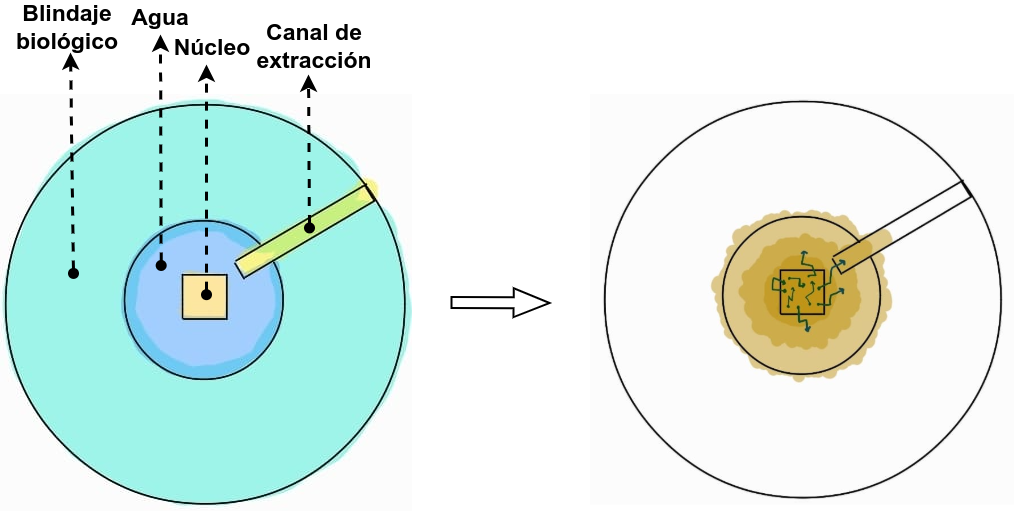
\includegraphics[width=0.8\textwidth]{nucleo2.png}
    \caption{Representación esquemática del núcleo de un reactor tipo pileta con canal de extracción. Se observa el núcleo central, rodeado por agua y blindaje biológico, así como un canal de extracción de neutrones. El gradiente de color indica cualitativamente la distribución de la población neutrónica típica en simulaciones Monte Carlo desde el núcleo.}
    \label{fig:nucleo2}
\end{figure}


% Para mitigar esta problemática, se emplean técnicas de reducción de varianza. Entre ellas, destaca el método general del \emph{source biasing}, basado en re-muestrear las fuentes originales. Esta técnica consiste en reemplazar la distribución original de partículas por una estadísticamente equivalente, construida sobre una superficie intermedia estratégicamente seleccionada. De esta manera, las partículas transportadas tienen mayor probabilidad de contribuir eficientemente a los tallies seleccionados, mejorando la estadística en la región objetivo sin aumentar desproporcionadamente el tiempo de CPU.

Para mitigar esta problemática, se suelen emplear técnicas de reducción de varianza tales como:
\begin{itemize}

    \item \textbf{Separación geométrica del problema}: consiste en dividir la simulación en regiones contiguas, separando la fuente original de la región de interés mediante una superficie de interfaz. En esta superficie se registra la distribución de partículas en el espacio de fases y su peso estadístico. Esta información se emplea para construir una nueva fuente que se utiliza en una simulación posterior, permitiendo focalizar los recursos computacionales exclusivamente en la región de interés.
    
    \item \textbf{Ventanas de peso}: esta técnica define un rango aceptable de pesos estadísticos para las partículas en cada región del dominio. Aquellas con peso muy alto son divididas (\emph{splitting}) y las de peso muy bajo pueden ser descartadas con cierta probabilidad, controlando así la varianza espacialmente.
    
    \item \textbf{Ruleta rusa}: se utiliza para descartar partículas con bajo peso estadístico, preservando el valor esperado del cálculo. Cada partícula tiene una probabilidad de ser eliminada o de continuar con su peso ajustado en consecuencia.
    
    \item \textbf{Absorción implícita}: en lugar de eliminar partículas cuando son absorbidas, se les reduce su peso estadístico de acuerdo a la probabilidad de absorción, permitiendo que las partículas sobrevivan y continúen su historia.
\end{itemize}

% En este trabajo se desarrolló una técnica basada en la separación geométrica del problema, con el objetivo de restringir la simulación a la región de interés. Para ello, se establece una superficie de acople ubicada estratégicamente dentro del modelo, sobre la cual se registran un archivo de partícula generado durante una simulación inicial que abarca el núcleo del reactor. Este archivo permite construir una fuente distribucional que reproduce de forma estadísticamente equivalente las distribuciones originales en el espacio de fases ($\mathbf{E}$–$\mathbf{r}$–$\boldsymbol{\Omega}$), incluyendo también el peso estadístico de cada partícula.

% A continuación, se genera una nueva simulación que consiste en la región de interés, utilizando la fuente distribucional como fuente ubicada en la superficie de acople. Al concentrar el computo en la zona de interes se incrementa la eficiencia, ya que las partículas simuladas poseen una mayor probabilidad de contribuir efectivamente a las magnitudes físicas relevantes de estudio, sin necesidad de transportar todo el sistema desde la fuente original de núcleo.

% En particular, en este trabajo se desarrolla una técnica basada en la separación geométrica del problema, cuyo objetivo es desacoplar geometricamente el modelo, restringiendo la simulación a la región de interés. Para ello, se establece una superficie de acople en una ubicación intermedia dentro del modelo, sobre la cual se registra un archivo de partículas generado durante una simulación inicial. A partir de este archivo, se construyen una fuente distribucional que reproduce de forma estadísticamente equivalente las distribuciones originales en el espacio de fases. De esta manera, en la etapa subsiguiente se generan partículas directamente en la región de interés, aumentando la eficiencia del cálculo, sin necesidad de transportar todo el sistema desde el núcleo.

%  En particular, en este trabajo se utiliza una implementación que consiste en desplazar virtualmente la fuente original hacia posiciones intermedias más cercanas al área de interés. Esto se logra mediante la grabación de archivos de partículas (\textit{trackfiles}) en superficies estratégicamente ubicadas durante la simulación inicial, los cuales permiten luego construir fuentes sintéticas denominadas fuentes de distribucionales que poseen distribuciones estadísticamente equivalentes a las originales. De esta manera, las partículas generadas en etapas subsiguientes poseen una mayor probabilidad de contribuir a los tallies definidos, mejorando la estadística en la región de estudio sin aumentar desproporcionadamente el tiempo de \textit{CPU}.

% \section{Fuentes distribucionales – base conceptual}

% El método se implementa dividiendo el problema original en una sucesión de etapas consecutivas delimitadas por \emph{superficies de acople} $\{\mathcal{S}_{i}\}_{i=1}^{\,n-1}$. Durante cada etapa $i$, se simulan partículas desde la fuente original hasta la superficie $\mathcal{S}_{i}$, almacenándose las propiedades de cada partícula (\emph{tracks}) en el espacio de fases ($\mathbf{E}$–$\mathbf{r}$–$\boldsymbol{\Omega}$) y su peso estadístico. Estas superficies se definen en posiciones donde sea posible registrar suficientes partículas para construir una fuente secundaria representativa en un tiempo razonable.

% El método se implementa dividiendo el problema original en una sucesión de etapas consecutivas delimitadas por \emph{superficies de acople} ${\mathcal{S}{i}}{i=1}^{,n-1}$. En la primera etapa, las partículas se simulan directamente desde la fuente original hasta la superficie $\mathcal{S}{1}$, registrando sus propiedades (o \emph{tracks}) en el espacio de fases ($\mathbf{E}$–$\mathbf{r}$–$\boldsymbol{\Omega}$) junto con su peso estadístico. A partir de estos datos, se construye una fuente secundaria representativa en dicha superficie, la cual se emplea como condición inicial en la etapa siguiente. Así, en cada etapa $i > 1$, las partículas no se simulan desde la fuente original, sino desde una fuente sintetizada en la superficie $\mathcal{S}{i-1}$, desplazando progresivamente la fuente hacia la región de interés. Las superficies de acople se ubican en posiciones estratégicas donde sea posible registrar una estadística suficiente en un tiempo computacional razonable.

% A partir de las listas generadas, se estima la distribución multidimensional de las partículas en la superficie $\mathcal{S}_{i}$, preservando las correlaciones entre las variables mencionadas. Esta distribución estimada se utiliza luego como fuente inicial en la siguiente etapa ($i+1$). De este modo, la fuente se traslada progresivamente hacia la región objetivo, logrando la precisión requerida con un número considerablemente menor de historias que el método tradicional sin reducción de varianza.

El método desarrollado en este trabajo se basa en la separación geométrica del problema en dos regiones: una que contiene el núcleo del reactor, y otra que abarca exclusivamente la región de interés. Esta técnica se implementa mediante la división del modelo simulado en dos regiones, delimitadas por superficies de acople ubicadas estratégicamente dentro de la geometría. En una primera etapa, se realiza una simulación completa del núcleo hasta una superficie intermedia, donde se registran en una lista las propiedades de las partículas que la atraviesan, incluyendo su energía, posición, dirección ($\mathbf{E}$–$\mathbf{r}$–$\boldsymbol{\Omega}$), y su peso estadístico.

A partir de esta lista de partículas, se estima la distribución multidimensional en el espacio de fases utilizando histogramas multidimensionales. Esta estructura permite segmentar el conjunto original de datos mediante histogramas de baja resolución, llamados histogramas macro, que separan el espacio de fases en regiones donde las correlaciones entre variables se mantienen aproximadamente constantes. Sobre cada una de estas regiones, se construyen histogramas de mayor resolución —los histogramas micro— que aproximan la distribución de cada variable con mayor detalle. De este modo, se preservan tanto la forma general de la distribución como las correlaciones relevantes entre las variables registradas. A partir de esta estimación, es posible generar nuevas partículas que pertenezcan estadísticamente al mismo espacio de fases que la muestra original, obteniendo así una fuente sintética denominada fuente distribucional. Esta metodología se desarrolla en profundidad en el Capítulo \ref{cap:metodo_histogramas}, donde se describe el procedimiento implementado para su construcción.

% A partir de esta lista de partículas, se estima la distribución multidimensional en el espacio de fases utilizando histogramas multidimensionales jerárquicamente acoplados. Esta estructura permite preservar las correlaciones entre variables a través de un orden preestablecido de procesamiento, generando así una fuente sintética denominada fuente distribucional.

En la segunda etapa, esta fuente distribucional se utiliza como fuente de entrada para una nueva simulación, que consiste únicamente en la región de interés, excluyendo el núcleo y sus alrededores. Al concentrar el esfuerzo computacional en esta zona, se incrementa la eficiencia, ya que las partículas simuladas poseen una mayor probabilidad de contribuir a las magnitudes físicas relevantes de estudio.

% \emph{A su vez, además del método mencionado, en este trabajo también se hace uso del método de \textbf{ventanas de peso} como técnica complementaria de reducción de varianza.}

% El método consiste en dividir el problema en una sucesión de etapas consecutivas, delimitadas por superficies de acople, ubicadas estratégicamente a lo largo de la geometría simulada. En la primera etapa, las partículas se simulan desde la fuente original hasta la primer superficie, donde se registran sus propiedades en el espacio de fases ($\mathbf{E}$–$\mathbf{r}$–$\boldsymbol{\Omega}$) en un archivo denominado \textit{trackfile}. A partir de esta lista de partículas, se aproxima la distribución multidimensional preservando las correlaciones entre las variables, y se utiliza para generar una fuente secundaria en dicha superficie. Esta fuente es entonces utilizada en la siguiente etapa. El proceso se repite, trasladando progresivamente la fuente hacia la región de interés. 

En la Figura \ref{fig:nucleo4} se ejemplifica el proceso desarrollado para una simulación del núcleo de un reactor de investigación tipo pileta. Inicialmente, se realiza una simulación completa desde el núcleo, obteniendo una estadística adecuada en los alrededores del mismo, la cual se reduce considerablemente a medida que los neutrones penetran en el agua circundante. Este fenómeno se visualiza mediante un gradiente de colores. En esta simulación inicial, se define una superficie de registro en la entrada de un canal de extracción. Las partículas que atraviesan dicha superficie se registran en un archivo de partículas, el cual, mediante la metodología que se va a desarrollar en este trabajo, se procesa para definir una fuente distribucional. Posteriormente, esta fuente permite simular únicamente el canal de extracción, concentrando la estadística en dicha región sin necesidad de repetir la simulación completa desde el núcleo.

\begin{figure}[H]
    \centering
    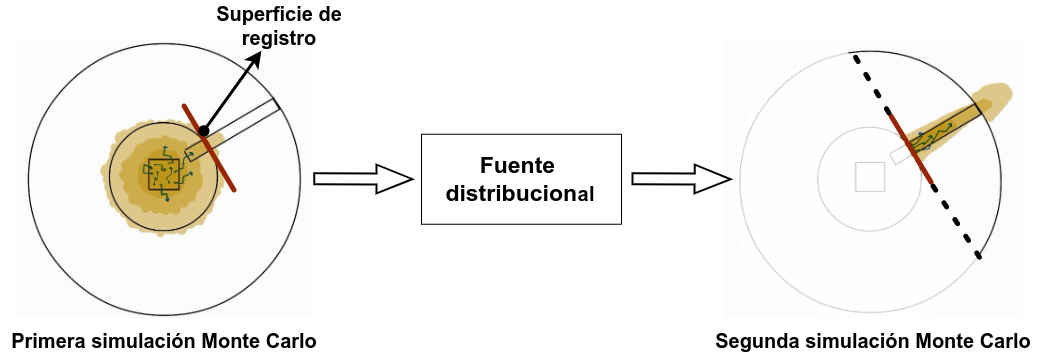
\includegraphics[width=\textwidth]{nucleo4.png}
    \caption{Esquema ilustrativo del proceso de desacople geométrico en simulaciones Monte Carlo para un reactor de investigación tipo pileta. En la primera etapa se registra un archivo de partículas en la entrada del canal de extracción, el cual es posteriormente utilizado para generar una fuente distribucional que permite simular eficientemente el canal de forma independiente. El gradiente de colores representa la disminución de la población neutrónica.}
    \label{fig:nucleo4}
\end{figure}

% \emph{Este enfoque permite alcanzar una buena precisión en zonas alejadas o poco accesibles, con un número considerablemente menor de historias simuladas en comparación con una simulación completa desde la fuente original.}

En resumen, el procedimiento consta de tres etapas fundamentales:

\begin{itemize}
    \item \textbf{Detección}: Registro de las variables del espacio de fases y del peso estadístico de cada partícula que atraviesa una superficie intermedia de desacople. El resultado de este proceso es un archivo de partículas que contiene la información necesaria para caracterizar la distribución de la fuente sobre dicha superficie.

    \item \textbf{Estimación}: Procesamiento del archivo de partículas mediante la metodología propuesta en este trabajo, basada en histogramas multidimensionales. Este procedimiento permite aproximar la distribución en el espacio de fases, preservando las correlaciones entre variables, y genera como resultado una fuente distribucional.

    \item \textbf{Producción}: Utilización de la fuente distribucional estimada para generar nuevas partículas que pertenezcan al espacio de fases del archivo de partículas original. Estas partículas son empleadas en simulaciones posteriores, permitiendo modelar la región de interés de forma desacoplada de la fuente original.
\end{itemize}

El archivo original de partículas contiene inevitablemente regiones del espacio de fases con baja estadística o sin eventos registrados, producto de su carácter finito. Si se reutiliza directamente como fuente en una simulación posterior —por ejemplo, simulando varias veces las mismas partículas registradas— se corre el riesgo de reproducir el mismo ruido estadístico, afectando la calidad de los resultados.

Para mitigar este problema, se emplea un procedimiento de estimación basado en histogramas multidimensionales que permite densificar el espacio de fases. En este enfoque, se utilizan histogramas para aproximar la distribución de variables, bajo el supuesto de que la probabilidad es constante dentro de cada bin. Esto habilita la generación de nuevas partículas en regiones que no estaban presentes explícitamente en el archivo original, completando así los vacíos estadísticos y asegurando una cobertura más uniforme del espacio de fases.

\section{Trabajos relacionados}

Los trabajos previos realizados en el Departamento de Física de Reactores y Radiaciones (DeFRRa) del Centro Atómico Bariloche (CAB) abordaron el modelado de fuentes distribucionales mediante el uso de histogramas multidimensionales \cite{Fairhurst2017Hist, Ayala2019Hist, Abbate2020Hist}. Esta estrategia permitió capturar correlaciones entre energía, posición y dirección en geometrías planas rectangulares, siendo aplicada satisfactoriamente en estudios vinculados al reactor RA‑10.

En continuidad con dichos desarrollos, la herramienta \texttt{KDSource} —también desarrollada en el DeFRRa— introdujo técnicas más avanzadas basadas en \textit{Kernel Density Estimation} (\textit{KDE}), en forma multivariante y adaptativa \cite{Abbate2021KDSource, Schmidt2022KDSourcePaper, Fox2022KDE, Gimenez2024KDSourceOpenMC}. \texttt{KDSource} permite ajustar automáticamente distribuciones continuas a partir de archivos de partículas previamente obtenidos y, a partir de ellas generar fuentes distribucionales, preservando las correlaciones del espacio de fases.

No obstante, el enfoque basado en \textit{KDE} presenta una limitación: su carácter inherentemente suavizante puede dificultar la representación precisa de discontinuidades abruptas en el espacio de fases. Estas discontinuidades pueden originarse, por ejemplo, en zonas de cambio de material o en la coexistencia de poblaciones de partículas con comportamientos físicos muy distintos, como neutrones térmicos isotrópicos mezclados con neutrones rápidos colimados. En estos casos, la suavización puede degradar la calidad de la fuente generada, especialmente cuando se busca preservar estructuras finas o anisotropías marcadas.

El presente trabajo extiende estas líneas incorporando los enfoques basados en histogramas multidimensionales dentro del entorno ya establecido de \texttt{KDSource}, proponiendo además un método de discretización adaptativa que automatiza la definición de las grillas de los histogramas macro y micro. A diferencia de los trabajos anteriores, este nuevo enfoque permite segmentaciones variables para diferentes subconjuntos del espacio de fases. Por ejemplo, el método puede asignar una discretización espacial más refinada para neutrones rápidos, donde suelen prevalecer anisotropías asociadas a haces colimados, y una discretización más homogénea para neutrones térmicos, cuya distribución tiende a ser más isotrópica. De esta forma, se logra preservar las correlaciones relevantes sin imponer una malla uniforme en todo el dominio, mejorando la capacidad de representación del método.

% No obstante, \textit{KDE} presenta una desventaja: su carácter inherentemente suavizante puede reducir la capacidad de representar adecuadamente discontinuidades abruptas presentes en ciertos problemas físicos relevantes.

% El presente trabajo extiende estas líneas incorporando los enfoques basados en histogramas multidimensionales dentro del entorno ya establecido de \texttt{KDSource}, proponiendo además un método de discretización adaptativa que automatiza la definición de las grillas de los histogramas macro y micro. A diferencia de los trabajos anteriores, este nuevo enfoque permite segmentaciones variables para diferentes subconjuntos del espacio de fases original. Por ejemplo, neutrones térmicos y rápidos pueden ser tratados con distinta resolución espacial, asignando automáticamente histogramas macros diferenciados en función de su energía. De forma análoga, la adaptabilidad también se extiende a los histogramas micro, permitiendo una resolución de la aproximación de las distribuciones condicionada por otras variables.

% Los desarrollos previos en el Departamento de Física de Reactores y Radiaciones (DeFRRa) del Centro Atómico Bariloche (CAB) han empleado histogramas anidados con discretización gruesa y fina (macro/micro-bins) para capturar adecuadamente las correlaciones entre energía, posición y dirección en fuentes planas rectangulares. Si bien este enfoque permitió resolver satisfactoriamente casos específicos relacionados con el reactor RA‑10, presenta limitaciones. Entre ellas, destacan la necesidad de definir manualmente las grillas de discretización, la poca suavidad inherente a los histogramas y las dificultades para tratar correctamente discontinuidades abruptas, como aquellas generadas por cambios de material o geometría.

% Posteriormente, la herramienta \texttt{KDSource} —desarrollada también en el DeFRRa— introdujo el uso de técnicas más avanzadas basadas en \textit{Kernel Density Estimation} (\textit{KDE}) multivariante adaptativa. El flujo de trabajo de \texttt{KDSource} comprende dos etapas diferenciadas: (i) una fase inicial de optimización \emph{off-line}, en la cual se ajusta automáticamente el modelo \textit{KDE} a partir de \textit{trackfiles} preexistentes, y (ii) una fase de muestreo \emph{on-the-fly}, donde un módulo integrado en \texttt{C}/\texttt{C++} genera nuevas partículas durante la simulación Monte Carlo manteniendo las correlaciones globales y la normalización del peso original. Este enfoque elimina la necesidad de manejar \textit{trackfiles} voluminosos durante la simulación, optimizando sustancialmente el uso de memoria \textit{RAM}.

% \begin{figure}[H]
%     \centering
%     
\includegraphics[width=0.5\textwidth]{figs/kdsource_logo.png}
%     \caption{Logo de \texttt{KDSource}. Fuente: \url{https://kdsource.readthedocs.io/en/latest/}}
%     \label{fig:kdsource_logo}
% \end{figure}



\section{Aportes específicos de este trabajo}

Este trabajo busca profundizar el desarrollo de \texttt{KDSource} mediante la incorporación de histogramas multidimensionales como una alternativa -o complemento- a la metodología \textit{KDE} existente. Las contribuciones específicas son:

\begin{itemize}
    \item Implementación de histogramas multidimensionales en \texttt{KDSource}, capaces de:
    \begin{itemize}
        \item preservar las correlaciones entre variables ($\mathbf{E}$–$\mathbf{r}$–$\boldsymbol{\Omega}$) para fuentes planas rectangulares;
        \item representar adecuadamente discontinuidades o picos en todas las variables;
        \item implementar un método de selección automática y adaptativa de bordes para los histogramas, tanto a nivel macro como micro, optimizado según la estadística disponible en cada subgrupo del espacio de fases.
    \end{itemize}

    \item Integración optimizada del flujo de trabajo en \texttt{OpenMC} mediante:
    \begin{itemize}
        \item generación \emph{offline} de un archivo intermedio en formato \texttt{XML} conteniendo la fuente distribucional, que incluye la información de los histogramas multidimensionales;
        \item desarrollo de un módulo en \texttt{C} que utilice eficientemente esta información para producir partículas individualmente;
        \item implementación de un remuestreo \emph{on-the-fly} integrado directamente en \texttt{OpenMC}, minimizando la ocupación de memoria al evitar la carga y gestión de archivos extensos de partículas.
    \end{itemize}

    \item Validación  del método en casos de complejidad creciente:
    \begin{itemize}
        \item Un caso simplificado, consistente en un haz colimado ingresando en un paralelepípedo de agua atravesado por un canal de vacío, con fuentes definidas artificialmente para permitir una comparación con una simulación directa más extensa sin la aplicación del método desarrollado. 
        \item Un caso real, consistente en la propagación a través del conducto Nº5 del reactor RA‑6, utilizando un archivo de partículas proporcionada por el departamento de Física de Neutrones del CAB generada a través de una simulación del núcleo en \texttt{OpenMC}.
    \end{itemize}
\end{itemize}




% \chapter{Introducción}

% \section{Contexto y motivación}

% Las simulaciones de transporte por metodo Monte Carlo son la herramienta de referencia cuando 
% la geometría y/o la anisotropía angular hacen inviables los métodos determinísticos. 
% Sin embargo, a medida que las partículas atraviesan blindajes o regiones muy absorbentes,
%  la estadística en la zona de interés se vuelve escasa y la incertidumbre de tallies, como
%   el flujo escalar por ejemplo, escala de forma prohibitiva con el tiempo de simulacion.
%   Para reducir el error estadistico sin multiplicar el tiempo de CPU se recurre a técnicas de 
%   reducción de varianza. Una de las más 
%    utilizadas es el re-muestreo de fuentes (source biasing en sentido amplio), 
%    donde se reemplaza la fuente original por una distribución estadísticamente 
%    equivalente construida en una superficie intermedia. De este modo se transportan 
%    preferentemente las partículas con mayor probabilidad de contribuir a los tallies 
%    seleccionados.

% \section{Fuentes distribucionales – base conceptual}


% La metodología se lleva a la práctica dividiendo el problema original 
% en $n$ etapas de transporte contiguas, delimitadas por \emph{superficies 
% de acople} $\{\mathcal{S}_{i}\}_{i=1}^{\,n-1}$. Durante la etapa $i$ se 
% simulan todas las partículas desde la fuente hasta la superficie 
% $\mathcal{S}_{i}$ y se guarda la \emph{lista de tracks} asociada, es decir, 
% el vector de fase de cada partícula que atraviesa la superficie. 
% Estas superficies se eligen de modo que el número de tracks registrado 
% resulte estadísticamente representativo para construir una fuente secundaria 
% confiable.


% A partir de cada lista se obtiene una estimación de la distribución multidimensional de 
% las partículas sobre $\mathcal{S}_{i}$ —conservando las correlaciones entre energía, posición 
% y dirección— y esa distribución se utiliza como fuente al comenzar la etapa $i\!+\!1$. Así, 
% la fuente efectiva se relocaliza paso a paso hacia la región de detección y se alcanza la 
% precisión deseada con un número de historias considerablemente menor que el requerido en un 
% cálculo sin \emph{source biasing}.



% El procedimiento completo consta de tres etapas:

% \begin{itemize}
%     \item \textbf{Detección} – Se registran las partículas (tracks) que cruzan una 
%     superficie intermedia de desacople, la cual actúa como desacople entre las distintas etapas de la simulación Monte Carlo, y se almacenan sus coordenadas en el espacio de fases 
%     ($E$, $x$, $y$, $\mu$, $\phi$, peso).
%     \item \textbf{Estimación} – A partir de esa lista se aproxima la distribución 
%     conjunta y sus correlaciones.
%     \item \textbf{Producción} – Se muestrea esa distribución para generar tantas 
%     partículas como sea necesario en la simulación secundaria.
% \end{itemize}

% Los primeros desarrollos en el Departamento de Física de Reactores y Radiaciones emplearon
% histogramas anidados (macro/micro–bins) para capturar las correlaciones
% $E$–$x$–$y$–$\mu$–$\phi$ en fuentes planas rectangulares.  
% Si bien el método permitió resolver algunos casos de aplicación
% presentados en tesis previas vinculadas al RA‑10, la definición manual
% de grillas y la limitada suavidad de las curvas generadas plantean
% desafíos cuando aparecen discontinuidades fuertes —por ejemplo, en cambios
% bruscos de material a través de una interfase— y al trasladarlo a otras
% geometrías.

% KDSource —una herramienta creada en el DFRyR para el post‑procesamiento
% y re‑muestreo de listas de partículas— emplea desde su concepción la
% \textit{Kernel Density Estimation} (KDE) multivariante adaptativa.
% El flujo de trabajo estándar consta de dos etapas: (i) optimización
% \emph{off‑line}, donde a partir de la lista de tracks se ajusta un
% modelo KDE con selección automática de ancho de banda, y (ii) muestreo
% \emph{on‑the‑fly}, en el cual un módulo en \texttt{C}/\texttt{C++}
% integra ese modelo dentro del código Monte Carlo y genera
% partículas una a una, conservando las correlaciones globales
% $E$–$\mathbf{r}$–$\boldsymbol{\Omega}$ y la normalización original del peso.
% Gracias a esta separación, KDSource elimina la necesidad de manipular
% archivos voluminosos de tracks durante la simulación. No obstante, el carácter suavizante de
% KDE puede atenuar discontinuidades muy marcadas; por ello este trabajo
% propone un esquema de histogramas multidimensionales adaptativos que
% mantenga las ventajas del muestreo continuo pero ofrezca un control
% más explícito sobre la resolución local.

% \section{Aportes específicos de este trabajo}

% El proyecto profundiza el desarrollo de KDSource mediante la
% incorporación de histogramas multidimensionales adaptativos como
% alternativa —o complemento— a KDE, con el objetivo de reproducir con
% mayor fidelidad estructuras espectrales o espaciales abruptas sin perder
% la correlación global entre variables.

% \begin{itemize}
%     \item Implementar un método alternativo de histogramas multidimensionales adaptativos dentro de KDSource que:
%     \begin{itemize}
%         \item reproduzca adecuadamente las correlaciones $E$-$x$-$y$-$\mu$-$\phi$ en una fuente plana rectangular perpendicular al eje $z$;
%         \item conserve las discontinuidades espectrales y espaciales propias de interfaces o colimadores;
%         \item ofrezca un control explícito del compromiso resolución/estadística.
%     \end{itemize}
    
%     \item Integrar y optimizar el flujo de trabajo en \texttt{OpenMC}:
%     \begin{itemize}
%         \item Generar, en modo off-line, un archivo intermedio (XML + HDF5) que contiene los histogramas y metadatos de la distribución.
%         \item Construir un módulo en C que, utilizando esa información, produzca una partícula a la vez.
%         \item Integrar el muestreo directamente en el código fuente de OpenMC (modo on-the-fly), de forma que sólo se mantenga en RAM la información de los histogramas y se evite la creación y carga de listas voluminosas.
%     \end{itemize}
    
%     \item Validar la herramienta en dos etapas de dificultad creciente:
%     \begin{itemize}
%         \item un caso simplificado: haz colimado que ingresa en un paralelepípedo
%         de agua atravesado por un canal de vacío; la fuente en la entrada
%         del conducto es definida y muestreada libremente, lo que permite
%         comparar los resultados con una simulación directa sin reducción
%         de varianza;
%         \item un caso condicionado por la fuente: propagación, a lo largo del
%         conducto N.º 5 del RA‑6, de la lista de partículas obtenida por el
%         Grupo de Física de Neutrones a partir de una simulación de núcleo;
%         aquí la estadística está limitada por la lista original y se
%         evalúa el desempeño del método bajo esa restricción.
%     \end{itemize}
% \end{itemize}

\chapter{Herramientas utilizadas}
\label{cap:herramientas}

Este capítulo tiene por objetivo presentar y describir las herramientas computacionales utilizadas a lo largo de este trabajo. Específicamente, se abordará el programa \texttt{OpenMC}, los formatos de archivos usados (\texttt{MCPL} y \texttt{XML}), y los lenguajes de programación involucrados (\texttt{Python}, \texttt{C} y \texttt{C++}).

\section{\texttt{OpenMC}}

\texttt{OpenMC} es un programa de simulación Monte Carlo desarrollado inicialmente en el \textit{Massachusetts Institute of Technology} como \textit{software} de código abierto \cite{OpenMC2024}. Actualmente es mantenido por el \textit{Argonne National Laboratory} junto a una activa comunidad internacional que contribuye continuamente a su desarrollo y expansión. Está especialmente orientado al cálculo del transporte de neutrones y fotones, permitiendo tanto simulaciones de criticidad como simulaciones de fuente fija. En este trabajo se emplean exclusivamente simulaciones de fuente fija.

Una de las ventajas de \texttt{OpenMC} es su flexibilidad en la obtención de resultados. El código permite registrar diferentes magnitudes físicas como flujos, dosis, corrientes, espectros energéticos, etc., además de ofrecer la posibilidad de registrar partículas que atraviesan superficies definidas por quien utiliza el programa en un archivo de formato \texttt{HDF5} \cite{HDF5_2025} o \texttt{MCPL} \cite{MCPL2024}. Estos archivos almacenan información de las variables de las partículas, permitiendo su posterior análisis o reutilización para generar nuevas simulaciones. Asimismo, \texttt{OpenMC} incorpora técnicas avanzadas de reducción de varianza, como las ventanas de peso (\textit{weight windows}), que resultan fundamentales para reducir la incertidumbre estadística de los resultados en áreas de interés específico, técnica utilizada en este trabajo.

\section{\texttt{KDSource}}



\texttt{KDSource} es una herramienta computacional desarrollada en conjunto por CNEA e IB, cuyo objetivo principal es procesar archivos de partículas generados en simulaciones Monte Carlo para la construcción de nuevas fuentes distribucionales \cite{KDSource2024}. Su integración con \texttt{OpenMC} permite desacoplar geométricamente simulaciones complejas, facilitando significativamente el cálculo de transporte en geometrías difíciles o extensas.

El fundamento original de \texttt{KDSource} reside en la técnica \textbf{Kernel Density Estimation (KDE)}, una técnica estadística que permite estimar distribuciones continuas de variables a partir de muestras discretas, manteniendo la correlación existente entre ellas. 

\section{Formatos de listas de partículas: \texttt{MCPL} y \texttt{HDF5}}

En simulaciones Monte Carlo, es común registrar partículas que atraviesan una superficie o ingresan a una región de interés, generando lo que se conoce como una lista de partículas. Estos archivos permiten capturar el estado de cada partícula —incluyendo su energía, posición, dirección, peso estadístico y tipo de partícula— al momento de cruzar una superficie.

\texttt{OpenMC} emplea por defecto el formato \texttt{HDF5} para almacenar estas listas \cite{HDF5_2025}. Este formato binario jerárquico permite almacenar datos de manera eficiente, estructurada y accesible desde diversos lenguajes de programación. Sin embargo, su estructura está adaptada específicamente al ecosistema de \texttt{OpenMC}, dificultando su reutilización directa en otros códigos de transporte.

Con el objetivo de facilitar la interoperabilidad entre distintos códigos Monte Carlo, existe el formato \textbf{\texttt{MCPL} (\textit{Monte Carlo Particle List})} \cite{MCPL2024}. Este estándar de listas de partículas permite almacenar listas generadas en simulaciones de forma compacta y eficiente, preservando información esencial como la energía, posición, dirección, peso de cada partícula y tipo de partícula. A diferencia de formatos específicos como \texttt{HDF5}, \texttt{MCPL} fue concebido como una interfaz  entre diferentes entornos Monte Carlo.

La Figura \ref{fig:mcpl_support_diagram} muestra los diversos códigos que pueden producir o consumir archivos en formato \texttt{MCPL}. En este proyecto, su uso permite vincular eficientemente los archivos de partículas generados por \texttt{OpenMC} con la herramienta \texttt{KDSource}.

\section{Formato \texttt{XML}}

El formato \textbf{\texttt{XML} (\textit{Extensible Markup Language})} es un lenguaje utilizado para describir y almacenar información estructurada de manera jerárquica, basándose en una organización de datos tipo árbol \cite{XML2025}. Una de sus principales ventajas es que está diseñado para ser tanto legible por máquinas como por humanos, lo que facilita su edición, inspección y validación manual durante el desarrollo. Debido a estas características, resulta particularmente adecuado para guardar las distribuciones estimadas mediante histogramas multidimensionales. A su vez, \texttt{OpenMC} emplea archivos \texttt{XML} para almacenar la configuración completa de sus simulaciones (geometría, materiales, configuración de \textit{tallies}, etc.), por lo que la elección de este formato contribuye a una integración directa y eficiente entre los componentes desarrollados.

\begin{figure}[H]
    \centering
    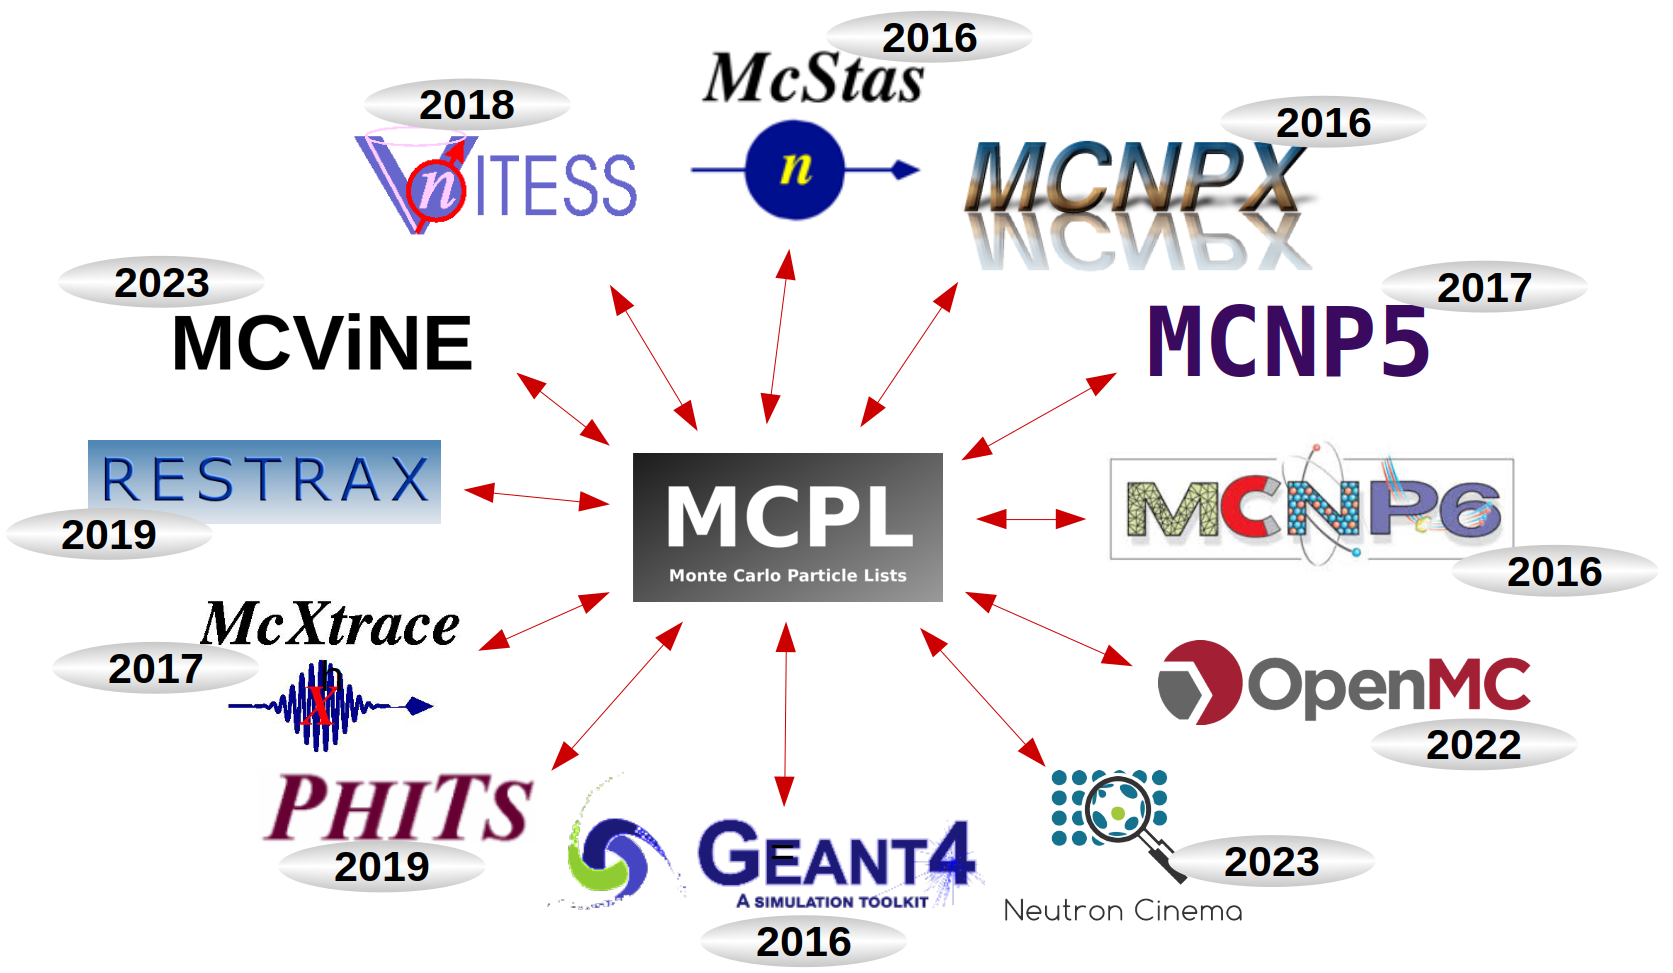
\includegraphics[width=\textwidth]{figs/mcpl_support_diagram.png}
    \caption[Diagrama de soporte de \texttt{MCPL}.]{Diagrama de soporte de \texttt{MCPL}. Reproducido de \cite{MCPL2024}.}
    \label{fig:mcpl_support_diagram}
\end{figure}

\section{Lenguajes de programación: \texttt{Python}, \texttt{C} y \texttt{C++}}

A lo largo del desarrollo del proyecto, se utilizaron principalmente tres lenguajes de programación:

\begin{itemize}
    \item \textbf{\texttt{Python}}: lenguaje de alto nivel especialmente adecuado para interfaces de usuario, análisis exploratorio de datos y configuración de simulaciones debido a su simplicidad, claridad y flexibilidad. \texttt{KDSource} hace uso de \texttt{Python} para la preparación y procesamiento de datos previos al remuestreo Monte Carlo. Tanto \texttt{KDSource} como \texttt{OpenMC} disponen de una interfaz en Python.

    \item \textbf{\texttt{C}}: lenguaje de programación de bajo nivel conocido por su eficiencia computacional, velocidad y control preciso sobre la gestión de memoria. Se utilizó en este trabajo para desarrollar módulos específicos encargados del remuestreo eficiente de partículas, especialmente cuando se requieren grandes volúmenes de datos. El módulo de remuestreo de \texttt{KDSource} está escrito en este lenguaje.
    
    \item \textbf{\texttt{C++}}: lenguaje de programación que extiende a \texttt{C} con capacidades de programación orientada a objetos. Esta arquitectura permite la expansión modular del código y facilita su mantenimiento. \texttt{OpenMC} está desarrollado en este lenguaje.


\end{itemize}


El desarrollo realizado en este trabajo implementa un flujo computacional para el uso de fuentes distribucionales en simulaciones Monte Carlo. Este flujo se compone de tres etapas principales: detección, procesamiento y producción, y aprovecha las capacidades de los lenguajes \texttt{Python}, \texttt{C} y \texttt{C++}.

\textbf{Detección}: se realiza mediante una simulación inicial en \texttt{OpenMC}, en la cual se registra un archivo de partículas sobre una superficie. Este archivo puede guardarse en formato \texttt{HDF5}, que es el formato nativo de \texttt{OpenMC}, y luego ser convertido al formato \texttt{MCPL} si se desea continuar con el procesamiento. Alternativamente, si \texttt{OpenMC} fue compilado con soporte para \texttt{MCPL}, puede generarse directamente en dicho formato. El archivo resultante se almacena en disco para su uso posterior. Este procedimiento se ilustra en la Figura \ref{fig:flujo_deteccion}.

\begin{figure}[H]
    \centering
    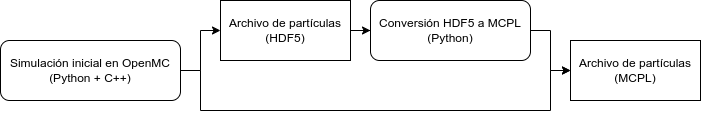
\includegraphics[width=0.75\textwidth]{flujo_codigos-Deteccion.png}
    \caption{Etapa de detección: registro de partículas en formato \texttt{MCPL} a partir de una simulación en \texttt{OpenMC}. Bloques con esquinas redondeadas representan procesos computacionales, mientras que los bloques rectangulares indican archivos que se registran o leen desde disco.}
    \label{fig:flujo_deteccion}
\end{figure}

\textbf{Procesamiento}: esta etapa se lleva a cabo en \texttt{Python} utilizando la implementación desarrollada para procesar mediante histogramas multidimensionales. A partir del archivo \texttt{MCPL}, se construye una fuente distribucional que representa la densidad de probabilidad estimada en el espacio de fases. El resultado de esta etapa es un archivo \texttt{XML}, que contiene la parametrización de la fuente y se almacena en disco como entrada para la etapa de producción. Este archivo \texttt{XML} constituye toda la información necesaria para generar nuevas partículas en simulaciones posteriores, sin requerir el acceso al archivo original de partículas. Esta característica representa una ventaja frente al método utilizado en \texttt{KDSource}, el cual necesita mantener el archivo original disponible en memoria durante la simulación posterior. Sin embargo, ambos métodos necesitan cargar en memoria el archivo de partículas original para el procesamiento. En casos donde dicho archivo posea un volumen considerable pueden derivar en un consumo elevado de memoria \textit{RAM}. La Figura \ref{fig:flujo_procesamiento} muestra un esquema de esta etapa.

\begin{figure}[H]
    \centering
    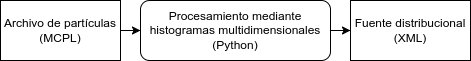
\includegraphics[width=0.55\textwidth]{flujo_codigos-Procesamiento.png}
    \caption{Etapa de procesamiento: construcción de una fuente distribucional a partir de un archivo \texttt{MCPL}. Bloques con esquinas redondeadas representan procesos computacionales, mientras que los bloques rectangulares indican archivos que se registran o leen desde disco.}
    \label{fig:flujo_procesamiento}
\end{figure}

\textbf{Producción}: esta etapa puede abordarse de dos maneras, implementada en código \texttt{C}. En la modalidad \textit{offline}, el archivo \texttt{XML} es utilizado para generar una nueva lista de partículas en formato \texttt{MCPL}, que luego puede emplearse directamente como fuente en \texttt{OpenMC} si se cuenta con soporte para este formato. En caso contrario, puede convertirse nuevamente a \texttt{HDF5}. En la modalidad \textit{on-the-fly}, se evita por completo el uso de listas intermedias: \texttt{OpenMC} accede directamente al archivo \texttt{XML} y realiza el remuestreo dinámicamente durante la simulación, gracias a una extensión \emph{ad-hoc} incorporada en este trabajo. Ambas modalidades se ilustran en la Figura \ref{fig:flujo_produccion}.

\begin{figure}[H]
    \centering
    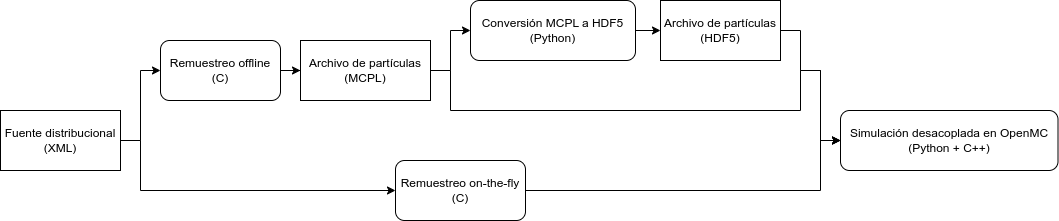
\includegraphics[width=\textwidth]{flujo_codigos-Remuestreo.png}
    \caption{Etapa de producción: uso del archivo \texttt{XML} para generar nuevas partículas de forma offline o on-the-fly. Bloques con esquinas redondeadas representan procesos computacionales, mientras que los bloques rectangulares indican archivos que se registran o leen desde disco.}
    \label{fig:flujo_produccion}
\end{figure}




\chapter{Metodología para la generación de fuentes Monte Carlo mediante histogramas multidimensionales}
\label{cap:metodo_histogramas}
\section{Introducción general al método}
La metodología propuesta se basa en el procesamiento de archivos de partículas generados en simulaciones Monte Carlo previas, específicamente usando \texttt{OpenMC}, para definir fuentes distribucionales para simulaciones subsiguientes.

\section{Definición del espacio de fases \texorpdfstring{$(\mathbf{E}$--$\mathbf{r}$--$\boldsymbol{\Omega})$}{(E--r--Omega)}}
Para aproximar correctamente las distribuciones y correlaciones del espacio de fases se consideraron seis variables para representar la energía, posición y dirección: tres coordenadas espaciales $(x, y, z)$, dos variables direccionales definidas en coordenadas esféricas ($\mu = \cos(\theta), \phi$) y una variable energética ($E$ o letargía $ln(E_0/E)$). En la Figura \ref{fig:terna} se observa una representación de las variables del espacio de fases. En situaciones como la considerada en este trabajo, donde la fuente se registra sobre una superficie plana, es posible rotar el sistema de coordenadas de modo que dicha superficie resulte perpendicular al eje $z$. Por lo tanto la coordenada $z$ permanece constante, permitiendo representar el espacio de fases con cinco variables.

\begin{figure}[h]
    \centering
    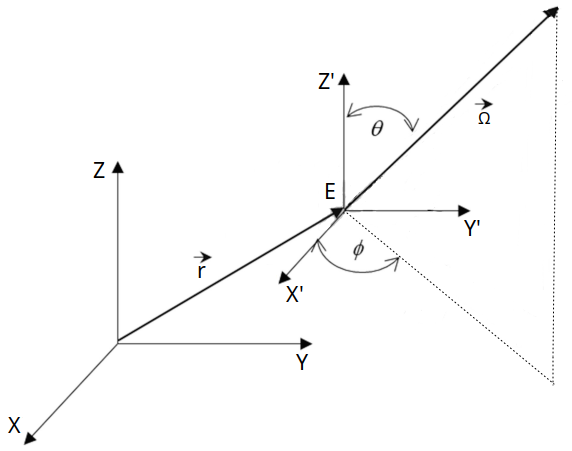
\includegraphics[width=0.5\textwidth]{figs/terna.png}
    \caption{Representación del espacio de fases con las variables $(E, x, y, z, \theta, \phi)$, donde $E$ es la energía, $x$, $y$ y $z$ son coordenadas espaciales y $\theta$ y $\phi$ son las variables direccionales.}
    \label{fig:terna}
\end{figure}

\section{Procesamiento del archivo de partículas original}
\subsection{Preprocesamiento del archivo de partículas}
Inicialmente, las partículas provenientes de la simulación Monte Carlo original se filtran seleccionando únicamente aquellas que se propagan hacia la región de interés y se separan las variables relevantes mencionadas, además del peso estadístico (\textit{weight}). Esta selección se realiza porque, en la siguiente etapa de simulación, la geometría considera un vacío en la región donde originalmente se encontraba la superficie de registro, permitiendo que únicamente las partículas que avanzan en dirección hacia la región de interés puedan ser simuladas. Las partículas que se dirigen en sentido opuesto no son relevantes para la simulación posterior, ya que en caso de que alguna partícula inicialmente dirigida hacia atrás fuese a regresar por retrodispersión, dicho comportamiento ya está estadísticamente incorporado en la lista original de partículas, producto de la simulación completa previa. En la Tabla \ref{tab:estructura_trackfile} se presenta un ejemplo de la estructura típica de un archivo de partículas.

\begin{table}[h]
    \centering
    \begin{tabular}{ccccccc}
        \toprule
        \textbf{Partícula Nº} & \textbf{Letargía} & \textbf{x [cm]} & \textbf{y [cm]} & \textbf{$\mu$} & \textbf{$\phi$ [rad]} & \textbf{Peso estadístico} \\ 
        \midrule
        1       & 4.15 &  0.23  & -1.10 &  0.85 & 3.14 & 1.00 \\
        2       & 4.95 & -0.75  &  0.40 & 0.65 & 1.57 & 1.00 \\
        3       & 5.05 &  1.10  &  0.70 &  0.45 & 0.78 & 1.00 \\
        4       & 5.30 & -0.50  & -0.90 &  0.60 & 2.35 & 1.00 \\
        5       & 4.85 &  0.85  & -0.20 & 0.95 & 1.25 & 1.00 \\
        $\vdots$ & $\vdots$ & $\vdots$ & $\vdots$ & $\vdots$ & $\vdots$ & $\vdots$ \\[0.2cm]
        100000  & 5.00 &  0.10  &  0.55 & 0.70 & 0.95 & 1.00 \\
        \bottomrule
    \end{tabular}
    \caption{Ejemplo ilustrativo de la estructura típica de un archivo de partículas. El archivo original suele contener cientos de miles de partículas.}
    \label{tab:estructura_trackfile}
\end{table}

\subsection{Utilización de histogramas macro y micro}
La metodología desarrollada en este trabajo para aproximar distribuciones y correlaciones multidimensionales en el espacio de fases de partículas provenientes de simulaciones Monte Carlo se basa en un esquema combinado de histogramas macro y micro. Esta aproximación permite gestionar eficientemente grandes volúmenes de datos manteniendo una representación precisa de la información esencial del conjunto original de partículas.

Los histogramas macro son subdivisiones jerárquicas del espacio de fases, realizadas siguiendo un orden determinado por el usuario. Por ejemplo, un posible orden es la \textit{letargía}, seguida por las coordenadas espaciales (\textit{X}, \textit{Y}), y posteriormente por la dirección (\textit{$\mu$}, \textit{$\phi$}). Este procedimiento inicia dividiendo el conjunto original de partículas en macrogrupos según la primera variable elegida (por ejemplo, \textit{letargía}). Cada macrogrupo así generado es posteriormente subdividido en nuevos macrogrupos en función de la siguiente variable (por ejemplo, la coordenada \textit{X}), repitiéndose este proceso de manera iterativa para cada variable subsiguiente. El resultado es una estructura jerárquica en forma de árbol, donde cada rama representa un subconjunto específico del archivo original de partículas, ya que incluye las cinco variables consideradas. Cada nodo en la rama corresponde a  una variable dentro de dicho subconjunto. En la Figura \ref{fig:estructura_jerarquica} se ilustra este procedimiento de subdivisión jerárquica del espacio de fases.

\begin{figure}[h]
    \centering
    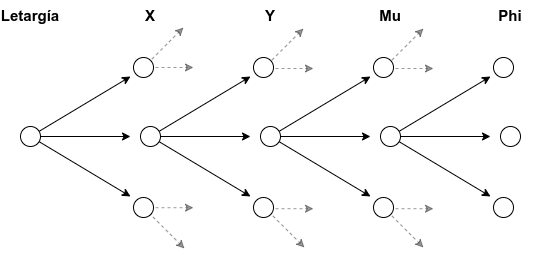
\includegraphics[width=0.8\textwidth]{grupos.png}
    \caption{Esquema ilustrativo de la estructura jerárquica de macrogrupos y microgrupos formando un árbol. Se resalta claramente la jerarquía entre variables.}
    \label{fig:estructura_jerarquica}
\end{figure}

Este esquema tiene como objetivo capturar las correlaciones entre las variables del espacio de fases. Cada nodo o macrogrupo resultante comparte similitudes en todas las variables consideradas hasta ese nivel jerárquico. Por ejemplo, un macrogrupo particular tendrá partículas con distribuciones similares en \textit{letargía}, coordenadas espaciales (\textit{X}, \textit{Y}), y dirección \textit{($\mu$)}, lo cual garantiza que la distribución restante en la última variable \textit{($\phi$)} refleje adecuadamente las correlaciones subyacentes en los datos.

Cabe destacar que, en la etapa de macrodiscretización, se utilizan histogramas con baja resolución debido al crecimiento exponencial en la cantidad total de grupos generados, dado que el número total de macrogrupos es producto del número de divisiones en cada variable. Un número excesivamente alto de divisiones podría conducir a subconjuntos con muy pocas partículas, comprometiendo la calidad estadística.

Una vez establecidos los macrogrupos, cada nodo es discretizado con histogramas micro, los cuales poseen una mayor resolución para representar detalladamente la distribución de cada variable dentro del subconjunto. Sin embargo, es crucial controlar esta resolución para evitar reproducir el ruido estadístico presente en los datos originales, especialmente cuando se cuenta con un número reducido de partículas en el subconjunto.

La combinación de histogramas macro y micro permite obtener una aproximación eficiente y precisa de la distribución multidimensional del conjunto original, conservando las correlaciones entre las variables del espacio de fases. Esta estructura de histogramas multidimensionales representa, en síntesis, la información esencial extraída del archivo original de partículas para ser utilizada en simulaciones posteriores.

\subsection{Métodos de discretización aplicados a histogramas macro y micro}
En este trabajo se desarrollaron dos métodos de discretización (bineado) aplicables tanto a los histogramas macro como a los micro. El primero es el \textit{bineado uniforme}, que consiste en dividir la distribución de la variable en estudio utilizando bines equiespaciados. Este método tiene la ventaja de ser sencillo y rápido en su implementación, pero presenta la desventaja de no poder capturar adecuadamente cambios abruptos o picos aislados en las distribuciones.

El segundo método, denominado \textit{bineado adaptativo}, consiste en realizar inicialmente un bineado uniforme con una cantidad moderada de bines especificada por el usuario. Luego, este bineado inicial se refina iterativamente agregando nuevos bines donde la distribución estimada difiere en mayor medida respecto a la distribución original. El criterio para añadir un nuevo bin se basa en la comparación de la función de distribución acumulada (FDC) del bineado actual con la FDC de la distribución original calculada con alta resolución. En cada iteración, se identifica el punto con la mayor diferencia absoluta entre ambas FDC, donde se coloca un borde de bin adicional. En el \textbf{Apendice B} se presenta un ejemplo de la implementación de este método.

Este enfoque adaptativo permite asignar mayor resolución donde existe una mayor cantidad de peso estadístico, y menor resolución donde el peso es escaso, logrando así un mejor seguimiento de las zonas críticas y un adecuado suavizado en regiones con poca estadística.

Además, debido a que la cantidad de partículas generalmente disminuye al profundizar en las ramas del árbol jerárquico, puede ser necesario utilizar una resolución decreciente en las discretizaciones, tanto para los histogramas macro como para los micro, lo cual también ha sido implementado en este trabajo.

Finalmente, en aquellos casos en que el usuario conozca previamente la existencia de cambios abruptos o picos específicos en la distribución, es posible informar manualmente al método sobre la ubicación de estos fenómenos, estableciendo bordes de bin específicamente en esos puntos para mejorar la precisión de la discretización.


% \section{Aproximación de distribuciones mediante histogramas micro}

% Las distribuciones de las variables en el espacio de fases pueden representarse, de forma general, mediante histogramas. La elección del método de discretización (bineado) es crucial y condiciona la calidad de la aproximación obtenida. Los tres esquemas de bineado utilizados en este trabajo son:

% \begin{itemize}
%     \item \textbf{Bineado de igual separación}: Divide el rango completo de la variable en intervalos de ancho constante. 

%     \item \textbf{Bineado de igual integral}: Divide el rango en intervalos que contienen aproximadamente la misma cantidad de peso estadístico, generando así bines de tamaño variable. Este método logra una representación más eficiente en términos estadísticos, especialmente en regiones donde la densidad cambia abruptamente.

%     \item \textbf{Bineado adaptativo}: Divide el rango utilizando una discretización iterativa que asigna mayor resolución a las zonas de alta densidad estadística y menor resolución en regiones escasamente pobladas, con el objetivo explícito de reducir el ruido estadístico manteniendo manteniendo resolución en los cambios abruptos de la distribución.
% \end{itemize}

% En este trabajo se profundiza particularmente sobre el método de bineado adaptativo. El procedimiento propuesto se realiza en dos etapas principales:

% \begin{enumerate}
%     \item \textbf{Aproximación inicial gruesa}: Se discretiza la distribución con una cantidad reducida de bines uniformemente distribuidos, típicamente utilizando cerca del 25\% del número final previsto de bines, aunque puede ser definido por el usuario.
    
%     \item \textbf{Refinamiento iterativo}: En cada iteración se evalúa la diferencia absoluta entre la distribución acumulada estimada (FDC) aproximada mediante los bines actuales y la FDC de referencia calculada con muchos bines. Se agregan bines adicionales precisamente en las regiones donde esta diferencia es máxima, mejorando progresivamente la calidad del histograma resultante.
% \end{enumerate}

% Esta estrategia adaptativa permite capturar adecuadamente las regiones críticas de la distribución, proporcionando un balance controlado entre resolución local y suavidad global.

% \section{Aproximación de distribuciones mediante histogramas adaptativos}
% La distribución de cada variable es representada mediante histogramas con bines de ancho no uniforme, seleccionados mediante una técnica de \textit{binning} adaptativo. Este procedimiento asigna mayor resolución a regiones del espacio de fases con mayor densidad estadística y menor resolución en regiones de baja estadística, con el fin de reducir el ruido estadístico.

% El proceso adaptativo se realiza en dos etapas principales:
% \begin{enumerate}
%     \item Una aproximación gruesa con una cantidad inicial de bines uniformes (aproximadamente el 25\% del total).
%     \item Ajuste iterativo agregando nuevos bines donde la diferencia absoluta entre la distribución acumulada estimada (CFD) y la distribución acumulada real (calculada con un gran número de bines) es mayor.
% \end{enumerate}


% \section{Mantenimiento de correlaciones mediante histogramas macro}

% El algoritmo desarrollado permite preservar las correlaciones entre variables del espacio de fases a través de divisiones sucesivas del conjunto de datos. Este proceso admite tres esquemas posibles de bineado para cada variable: de igual separación, de igual integral o adaptativo. En todos los casos, la variable considerada se utiliza para dividir el conjunto de partículas actual en subgrupos o \emph{macrogrupos}, que son luego tratados recursivamente.

% Particularmente, en el caso del bineado adaptativo, el procedimiento comienza con una partición inicial de baja resolución distribuidos uniformemente y se aplica un refinamiento iterativo utilizando un criterio similar al empleado en la sección anterior: se identifican las regiones donde la separación entre la distribución acumulada empírica y la distribución acumulada de referencia es mayor, y se subdividen esas regiones para aumentar la resolución local.

% Este proceso de partición se aplica a cada variable en un orden definido por el usuario, generando una estructura en forma de árbol. En cada nodo del árbol se almacena la distribución acumulada de la variable correspondiente a ese nivel, junto con las fronteras de los macrogrupos definidos. Esta estructura permite preservar las correlaciones multidimensionales entre variables, ya que cada división se realiza condicionada a las divisiones previas.


% \section{Mantenimiento de correlaciones mediante macrogrupos}
% Para preservar la correlación entre variables, se utiliza una estrategia basada en la división secuencial del conjunto de datos en macrogrupos, comenzando con una división gruesa en cuatro subconjuntos y luego refinándola iterativamente mediante el procedimiento adaptativo hasta alcanzar la cantidad deseada de macrogrupos.

% Este proceso jerárquico y secuencial se aplica iterativamente a cada una de las variables del espacio de fases, dando lugar a una estructura de árbol donde cada nodo contiene información sobre la distribución acumulada de la variable correspondiente.

% En la figura \ref{fig:estructura_jerarquica} se muestra un esquema ilustrativo de la distribución jerárquica en macrogrupos. En este caso, la letargía constituye la primera variable que se procesa y se subdivide en distintos macrogrupos en la variable X. A continuación, cada uno de estos macrogrupos en X es nuevamente dividido en macrogrupos en la variable Y. Este procedimiento se repite para las variables subsiguientes, como Y y $\mu$. De este modo, cada nodo en la estructura representa un subconjunto específico del archivo de particulas original. Posteriormente, cada subconjunto es aproximado mediante un histograma micro, permitiendo obtener una estimación detallada de la distribución asociada a ese subconjunto.



\section{Remuestreo de partículas en simulaciones Monte Carlo subsecuentes}
El proceso de generación de partículas a partir de la información guardada en los histogramas multidimensionales implica:
\begin{enumerate}
    \item Generar un número pseudoaleatorio entre 0 y 1.
    \item Interpolar dicho número en la distribución acumulada normalizada de la variable raíz del árbol.
    \item Avanzar secuencialmente por las ramas del árbol determinando valores de las variables subsecuentes hasta obtener un conjunto completo de variables del espacio de fases.
\end{enumerate}

En la Figura \ref{fig:esquema_generacion_particulas} se ejemplifica el proceso de generación de partículas descrito previamente. En el caso particular de trabajar con cinco variables, se repetirá la generación de números pseudoaleatorios cinco veces consecutivas, obteniéndose así los cinco valores correspondientes de las variables. Cabe destacar que durante el remuestreo de la quinta variable no se generará un macrogrupo adicional, dado que esta es la última variable a muestrear y no existen más niveles en el árbol.

\begin{figure}[H]
    \centering
    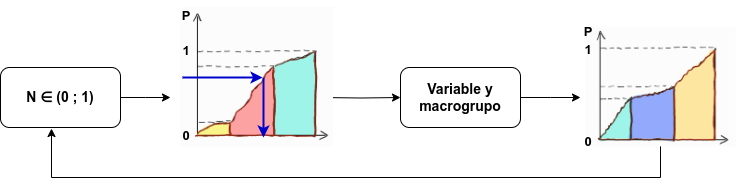
\includegraphics[width=\textwidth]{esquema5.png}
    \caption{Esquema ilustrativo del proceso secuencial de generación de partículas a partir de la distribución jerárquica guardada, resaltando el muestreo sucesivo mediante números pseudoaleatorios.}
    \label{fig:esquema_generacion_particulas}
\end{figure}

% Este enfoque evita la necesidad de cargar grandes listas en memoria \textit{RAM} durante la ejecución de simulaciones Monte Carlo, lo que simplifica considerablemente el manejo de fuentes en \texttt{OpenMC}.

% Este enfoque permite generar partículas para una siguiente simulación Monte Carlo. 

A través de este proceso es posible remuestrear nuevas partículas para la siguiente etapa de la simulación. Existen dos formas de integrar esta funcionalidad con \texttt{OpenMC}:

\begin{itemize}
    \item Una opción consiste en realizar, de forma \emph{offline}, el muestreo de una cantidad predeterminada de partículas y guardar sus propiedades en un archivo de partículas. Este archivo puede ser luego utilizado por \texttt{OpenMC} mediante su opción de simulación desde el modo de fuente \textit{FileSource} implementado en el programa.
    
    \item Alternativamente, se puede ejecutar \texttt{OpenMC} con una fuente del tipo \texttt{HistogramSource}, definida \textit{ad hoc} y configurada mediante un archivo \texttt{XML}. En este caso, \texttt{OpenMC} accede directamente al árbol de histogramas durante la simulación y genera cada partícula \emph{on-the-fly}, lo que reduce significativamente el uso de memoria y evita la necesidad de almacenar archivos de partículas intermedios voluminosos.
\end{itemize}

Esta funcionalidad fue incorporada en el contexto del presente trabajo, mediante la definición de una nueva clase de fuente en el código fuente de \texttt{OpenMC} en \texttt{C++}. Se desarrollaron las estructuras necesarias en \texttt{C} para efectuar el muestreo desde histogramas multidimensionales, y se integraron con la \texttt{API} de \texttt{OpenMC} en \texttt{Python}, permitiendo así que los histogramas puedan ser cargados y utilizados dentro del flujo habitual de simulación. El objetivo principal de esta implementación es facilitar el uso práctico de la herramienta.


\section{Implementación computacional}

La implementación computacional de la metodología descrita en este capítulo se encuentra desarrollada y documentada en el \textbf{Apendice A}. En particular, se presentan los códigos elaborados en \texttt{Python}, \texttt{C} y \texttt{C++} que posibilitan la generación y manejo de los histogramas multidimensionales generados a partir del archivo original de particulas. Dichos histogramas se configuran mediante parámetros específicos definidos por el usuario, tales como número y tipo de bines, así como el orden en que se procesan las variables del espacio de fases.

Asimismo, se documenta en detalle la integración realizada con \texttt{OpenMC}, incluyendo las modificaciones llevadas a cabo en su \textit{API} de \texttt{Python} y en su código fuente en \texttt{C++}, para permitir la generación \textit{on-the-fly} de partículas durante las simulaciones Monte Carlo subsecuentes.



% \section{Implementación computacional}
% La metodología descrita para estimar las distribuciones y correlaciones del \textit{trackfile} ha sido implementada en \texttt{Python}, debido a su leve/moderado costo computacional, creando una rutina que permite configurar parámetros tales como el número de bines y tipo de bineado para los histogramas macro y micro para cada variable, como así también el orden de procesamiento de las mismas. Esta rutina también ofrece la opción de insertar bordes manuales en los histogramas macro cuando se dispone de información previa que optimice la estimación.

% La estructura generada (árbol jerárquico de histogramas multidimensionales) es almacenada en un archivo \texttt{XML}, formato ideal debido a la estructura tipo árbol del dato generado. Posteriormente, esta información es utilizada directamente como fuente en simulaciones Monte Carlo subsecuentes en \texttt{OpenMC}, mediante modificaciones específicas realizadas tanto en su \textit{API} de \texttt{Python} como en su código fuente en \texttt{C++}.

% % \section{Conexión con la implementación computacional}
% La metodología expuesta fue implementada mediante códigos desarrollados en \texttt{Python}, \texttt{C} y \texttt{C++}, integrados específicamente dentro de los entornos de simulación Monte Carlo \texttt{OpenMC} y \texttt{KDSource}. La implementación detallada y comentada de estos códigos se presenta en el \textbf{Anexo A}, mostrando de forma explícita cómo se lleva a la práctica el proceso descrito anteriormente.

% En los capítulos siguientes el desempeño del método descrito será evaluado para cuantificar el grado en que el método conserva las propiedades originales del \textit{trackfile} registrado.

% \chapter{Evaluación del Método mediante Resampleo en \emph{Trackfiles}}
\label{chap:evaluacion-trackfiles}

\paragraph{Configuración 2: binning adaptativo (adaptive/adaptive).}  
Al aplicar binning adaptativo tanto en los macrogrupos como microgrupos, se optimiza la ubicación de los bordes para reflejar mejor la densidad local. En letargia se observa una mejora sustancial en la representación de los valores tipo delta, aunque persisten irregularidades en las zonas de letargia alta. Las variables espaciales muestran una mayor suavidad local sin perder detalle global.

Las métricas KL mejoran drásticamente respecto del caso uniforme:

\begin{center}
\begin{tabular}{lcc}
\toprule
\textbf{Configuración} & $\sum$KL 1D [nats] & $\sum$KL 2D [nats] \\
\midrule
Adaptive / Adaptive & 0.533 & 10.15 \\
\bottomrule
\end{tabular}
\end{center}

\paragraph{Configuración 3: macrobinning adaptativo, microbinning uniforme.}  
Esta variante mejora parcialmente la resolución estructural de la distribución, especialmente en 2D, pero mantiene el error en 1D cuando hay discontinuidades abruptas. Esto se refleja en un KL total intermedio:

\begin{center}
\begin{tabular}{lcc}
\toprule
\textbf{Configuración} & $\sum$KL 1D [nats] & $\sum$KL 2D [nats] \\
\midrule
Adaptive / Equal & 1.087 & 12.56 \\
\bottomrule
\end{tabular}
\end{center}

\paragraph{Configuración 4: macrobinning uniforme, microbinning adaptativo.}  
Esta última configuración aún no ha sido evaluada en detalle, pero se espera que muestre un comportamiento intermedio entre los casos previos. Se incluirá su análisis en una versión posterior.



\section{Resultados con Trackfile 1}
\label{sec:resultados-track1}

En esta sección se presentan los resultados obtenidos al aplicar el método sobre el primer archivo de tracks. El análisis se realizó utilizando múltiples configuraciones, variando el orden de las variables, la cantidad de macrogrupos y microgrupos.

Se muestran:

\begin{itemize}
    \item Distribuciones de energía, posición y dirección reconstruidas y su comparación con las originales.
    \item Curvas de error relativo por variable.
    \item Mapas de error relativo 2D para las correlaciones seleccionadas.
    \item Tabla con valores de divergencia KL para distintas configuraciones.
\end{itemize}

Estos resultados permiten discutir la sensibilidad del método a cada uno de los parámetros de entrada y establecer lineamientos para su elección óptima.

\subsection{Comparación entre esquema adaptativo y de ancho constante}
\label{subsec:adaptativo-vs-constante}

Como parte del análisis sobre el primer trackfile, se estudió el impacto del esquema de discretización utilizado en los macro y microgrupos. Se comparó explícitamente el rendimiento del esquema adaptativo frente a un esquema de histogramas con ancho constante.

El esquema adaptativo asigna mayor resolución a regiones del espacio de fases con alta estadística, y menor resolución donde los datos son escasos. Esto permite representar con mayor fidelidad las distribuciones sin amplificar el ruido estadístico.

Los resultados muestran una mejora significativa en la reconstrucción cuando se utiliza el esquema adaptativo. Esto se evidencia tanto en los gráficos de error relativo como en los valores de la divergencia KL, donde se observa una reducción consistente al aplicar el bineado adaptativo.

Esta comparación resalta la importancia de emplear técnicas de bineado adaptativo como herramienta para preservar la calidad del muestreo, especialmente en regiones con estructuras finas y alta variabilidad estadística.

\section{Resultados con Trackfile 2}
\label{sec:resultados-track2}

Se repitió el procedimiento metodológico sobre un segundo archivo de tracks con características geométricas y espectrales diferentes al primero, lo cual permite poner a prueba la generalidad del método propuesto.

Al igual que en el caso anterior, se analizaron distintas configuraciones de discretización jerárquica y orden de variables, prestando especial atención a:

\begin{itemize}
    \item La estabilidad del método ante distribuciones menos suaves o más concentradas espacialmente.
    \item La sensibilidad de las correlaciones bidimensionales al cambio en el esquema de macrogrupos.
    \item El comportamiento de la divergencia KL como función de la resolución utilizada.
\end{itemize}

Los gráficos comparativos muestran una buena reconstrucción general de las distribuciones 1D, aunque se observaron mayores errores relativos en regiones de baja estadística. En cuanto a las correlaciones, se destaca nuevamente la importancia de evitar configuraciones con fragmentación excesiva en las últimas variables del árbol.

Se presenta a continuación una selección representativa de los resultados gráficos y numéricos obtenidos, incluyendo:

\begin{itemize}
    \item Plots de distribuciones originales vs. reconstruidas.
    \item Mapas de error relativo 2D para variables espaciales y angulares.
    \item Tabla comparativa de divergencias KL.
\end{itemize}

\begin{table}[H]
    \centering
    \caption{Divergencia KL para distintas configuraciones en Trackfile 2.}
    \begin{tabular}{lccc}
        \toprule
        \textbf{Configuración} & \textbf{Macrogrupos} & \textbf{Microgrupos} & \textbf{KL Divergence} \\
        \midrule
        Orden A & [8,8,8,8] & [80,80,80,80] & 0.021 \\
        Orden B & [6,7,8,9] & [60,70,80,90] & 0.016 \\
        Orden C & [9,8,7,6] & [100,80,60,40] & 0.019 \\
        \bottomrule
    \end{tabular}
    \label{tab:trackfile2_kl}
\end{table}


\section{Resultados con Trackfile 3}
\label{sec:resultados-track3}

Finalmente, se aplicó el método sobre un tercer archivo de tracks con características mixtas, presentando una distribución energética más extendida y un patrón angular complejo, lo cual representa un desafío adicional para el muestreo jerárquico.

Se realizaron pruebas similares a las anteriores, enfocándose en:

\begin{itemize}
    \item Evaluar la robustez del método frente a distribuciones con múltiples picos o simetrías rotas.
    \item Observar el efecto del esquema de macrogrupos decreciente en variables angulares.
    \item Validar si se mantiene la tendencia en la divergencia KL al aplicar bineado adaptativo.
\end{itemize}

Los resultados obtenidos son consistentes con los de los otros casos, aunque se observaron diferencias notables en la reconstrucción de las variables angulares cuando éstas se encontraban en posiciones tempranas dentro del árbol, lo cual sugiere una posible pérdida de fidelidad debido a fragmentación excesiva.

\begin{table}[H]
    \centering
    \caption{Divergencia KL en Trackfile 3 para diferentes combinaciones.}
    \begin{tabular}{lccc}
        \toprule
        \textbf{Configuración} & \textbf{Macrogrupos} & \textbf{Microgrupos} & \textbf{KL Divergence} \\
        \midrule
        Esquema uniforme & [6,6,6,6] & [60,60,60,60] & 0.024 \\
        Esquema creciente & [6,7,8,9] & [60,70,80,90] & 0.017 \\
        Esquema adaptativo & Variable & Adaptativo & 0.012 \\
        \bottomrule
    \end{tabular}
    \label{tab:trackfile3_kl}
\end{table}

Estos resultados reafirman la utilidad del esquema adaptativo en escenarios complejos, donde las estructuras locales en el espacio de fases requieren una resolución flexible para ser correctamente representadas.



\chapter{Validación del metodo implementado: canal de vacío rodeado por agua}

En el presente capítulo se verifica la implementación del método desarrollado para la generación de fuentes Monte Carlo mediante histogramas multidimensionales. El caso de estudio seleccionado consiste en un canal de vacío rodeado lateralmente por un bloque de agua liviana. El modelo implementado se detallará en la siguiente sección. El objetivo principal de esta sección es analizar el desempeño del método propuesto en términos de conservación del flujo escalar a lo largo del modelo, así como evaluar la preservación del espectro energético y la corriente neutrónica en diferentes regiones del canal. Se ha seleccionado este modelo debido a que es un problema sensible ante perturbaciones de la fuente, lo que permite evaluar la eficacia del método de remuestreo implementado.

Con el objetivo de verificar el método de remuestreo desarrollado, se realizó en primer lugar una simulación desde la entrada del modelo hasta una superficie de registro ubicada en una posición intermedia de la geometría. Esta simulación tuvo como único propósito generar un archivo de partículas, el cual será procesado para construir una fuente distribucional.

Posteriormente, se llevó a cabo una segunda simulación, también iniciada desde la entrada del sistema, pero extendida hasta una superficie ubicada más alejada. A diferencia de la anterior, esta simulación tuvo por objetivo obtener resultados de referencia para uso posterior: en particular, el perfil convergido del flujo escalar a lo largo del canal, así como la corriente y el espectro neutrónico incidente en la superficie más alejada. Estos resultados de referencia son utilizados en etapas posteriores del trabajo como base para la validación del método de remuestreo propuesto.

Finalmente, se procesó el archivo de partículas grabado en la superficie intermedia de la primera simulación para construir una fuente distribucional basada en histogramas multidimensionales. Esta fuente se utilizó en una tercera simulación iniciada directamente desde la posición intermedia, obteniendo así una estadística suficientemente convergida hasta la superficie más alejada. Esta última simulación permitió realizar una comparación directa con los resultados obtenidos en la segunda simulación, evaluando así el método de generación de fuentes implementado, tal como se resume esquemáticamente en la Figura~\ref{fig:esquema_remuestreo}.

\begin{figure}[h]
    \centering
    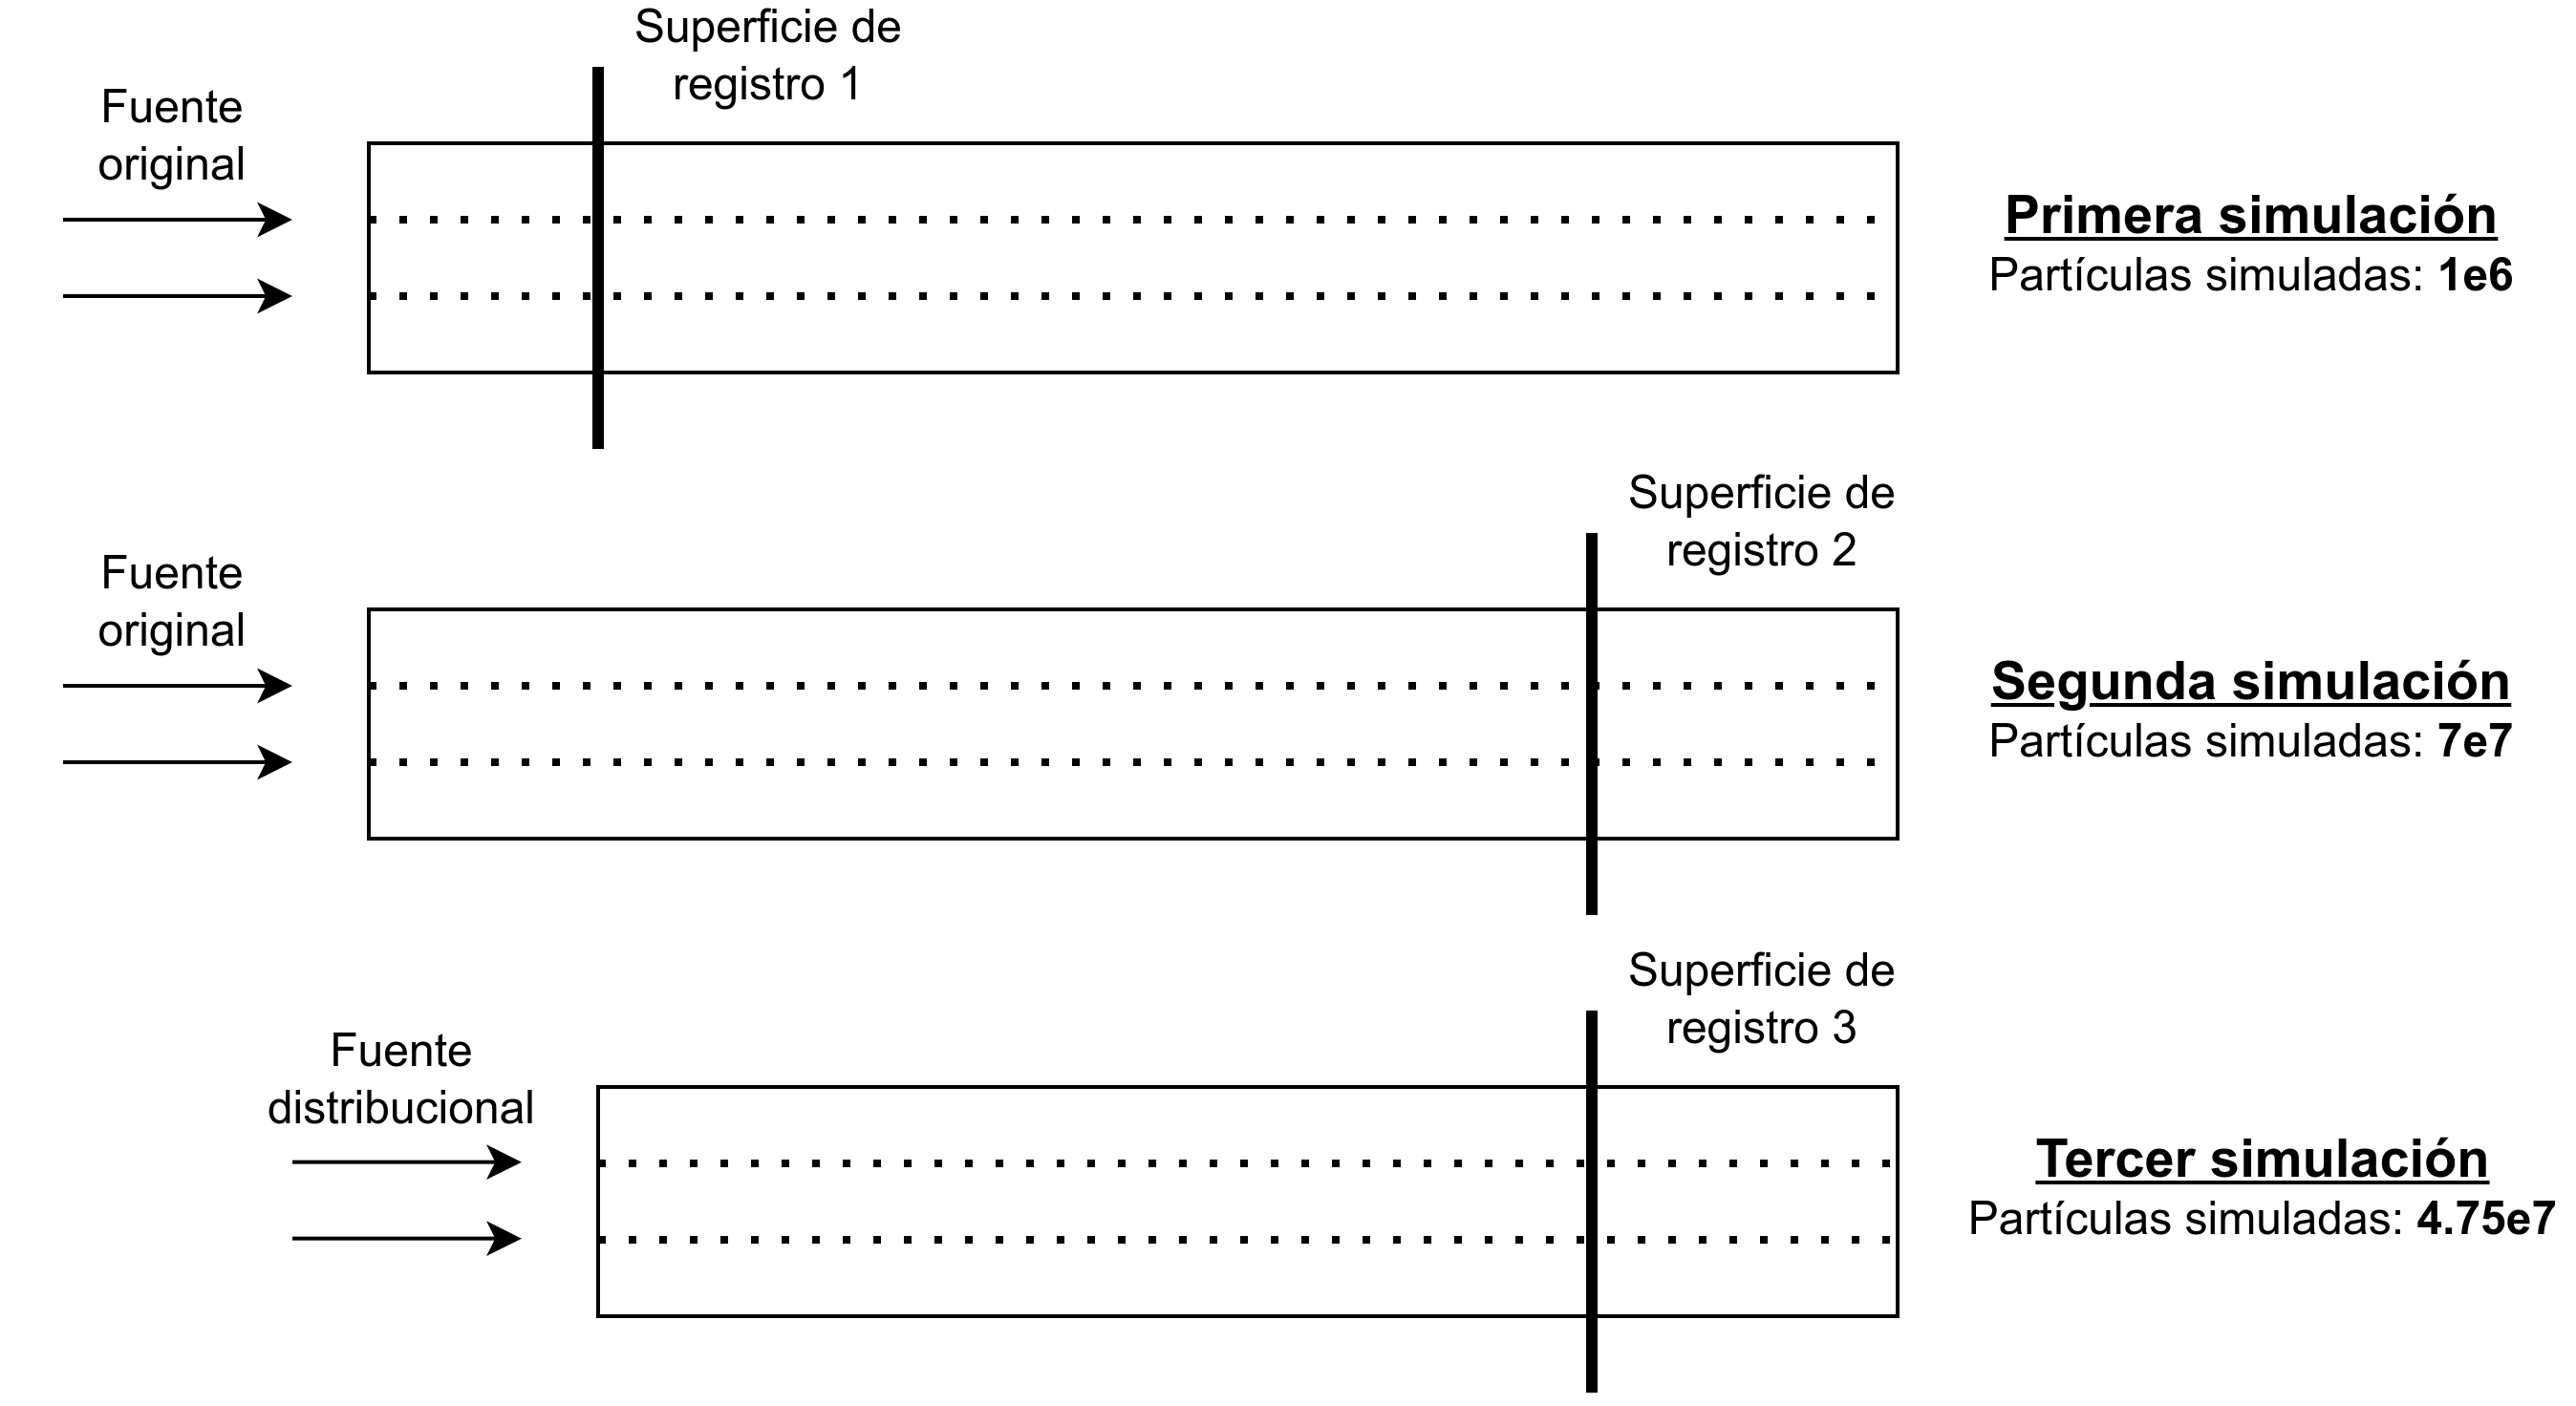
\includegraphics[width=\textwidth]{esquema_paralelepipedo.png}
    \caption{Esquema del proceso de remuestreo y validación del método implementado.}
    \label{fig:esquema_remuestreo}
\end{figure}

\section{Descripción del modelo simulado en \texttt{OpenMC}}

El modelo utilizado en las simulaciones consiste en un canal interno de vacío rodeado lateralmente por agua liviana. El sistema se diseñó como un paralelepípedo de agua con dimensiones $15\,\text{cm} \times 15\,\text{cm} \times 100\,\text{cm}$, que alberga en su interior un canal de vacío con sección transversal cuadrada de $3\,\text{cm} \times 3\,\text{cm}$, orientado en dirección del eje $z$. En la Figura \ref{fig:modelo_simulado_openmc} se presenta un esquema del modelo implementado en \texttt{OpenMC}.

\begin{figure}[h]
    \centering
    \includegraphics[width=\textwidth]{paralelepipedo_3.png}
    \caption{Esquema del modelo simulado en \texttt{OpenMC}.}
    \label{fig:modelo_simulado_openmc}
\end{figure}

La fuente de neutrones utilizada se definió sobre la cara de entrada del sistema (ubicada en $z = 0,\text{cm}$) y consistió en neutrones monoenergéticos con energía de $E = 1\,\text{MeV}$ y colimados en dirección del eje $z$ (con coseno direccional $\mu = \cos(\theta) = 1$). Esta configuración genera dos poblaciones de neutrones claramente diferenciadas: la primera, formada por neutrones que atraviesan el canal de vacío sin colisiones y mantienen tanto su energía inicial como su dirección; y la segunda, constituida por neutrones que interactúan con el moderador de agua, sufriendo dispersión angular y pérdida energética.

Para el análisis y posterior generación de la fuente, se registró un archivo de partículas sobre una superficie intermedia situada en $z = 15\,\text{cm}$. Este archivo contiene información sobre ambas poblaciones mencionadas, es decir, neutrones no colisionados y neutrones dispersados.

Durante las simulaciones se determinó el flujo escalar neutrónico a lo largo del canal, tanto dentro del canal de vacío como en el moderador circundante.

Para optimizar la estadística en regiones con baja presencia de partículas, particularmente en el agua, se implementó la técnica de ventanas de peso disponible en \texttt{OpenMC}. Este método actualiza los pesos de las partículas durante la simulación, permitiendo obtener mejorar estadística.

\section{Descripción del archivo de partículas original} 

El archivo de partículas fue registrado en una primera simulación del tubo de vacío desde el comienzo de la geometría. Corresponde a partículas registradas en una superficie ubicada a 15cm del inicio de la geometría. La lista contiene tanto neutrones que atraviesan la sección del canal, como neutrones que viajan por el agua. Sin embargo, la mayor proporción de peso estadístico se encuentra dentro del tubo de vacío, lo cual se corrobora tanto en la proyección $X$-$Y$, donde se observa una distribución más intensa contenida en un cuadrado correspondiente a la sección del tubo, como en la Tabla \ref{tab:particulas_pesos}, que presenta la cantidad de partículas y peso estadístico registrado por región. La Figura \ref{fig:trackfile1_x_y} muestra la proyección de los neutrones en el plano $X$-$Y$.

\begin{table}[H]
    \centering
    \begin{tabular}{lccccc}
        \toprule
        & & \multicolumn{2}{c}{Cantidad registrada [\#]} & \multicolumn{2}{c}{Densidad [\#/cm$^2$]} \\
        \cmidrule(lr){3-4} \cmidrule(lr){5-6}
        Región & Área [cm$^2$] & Partículas & Peso estad. & Partículas & Peso estad. \\
        \midrule
        Vacío & 9 & 62.523 & 46.862 & 6.947 & 5.207 \\
        Agua  & 216 & 390.412 & 44.938 & 1.807 & 208 \\
        \midrule
        Total & 225 & 452.935 & 91.800 & -- & -- \\
        \bottomrule
    \end{tabular}
    \caption{Resumen de partículas y peso estadístico registrados en la superficie intermedia ($z = 15$~cm) para cada región. Se informa también el área de cada región, así como la densidad de partículas y peso estadístico.}
    \label{tab:particulas_pesos}
\end{table}

\begin{figure}[H]
    \centering
    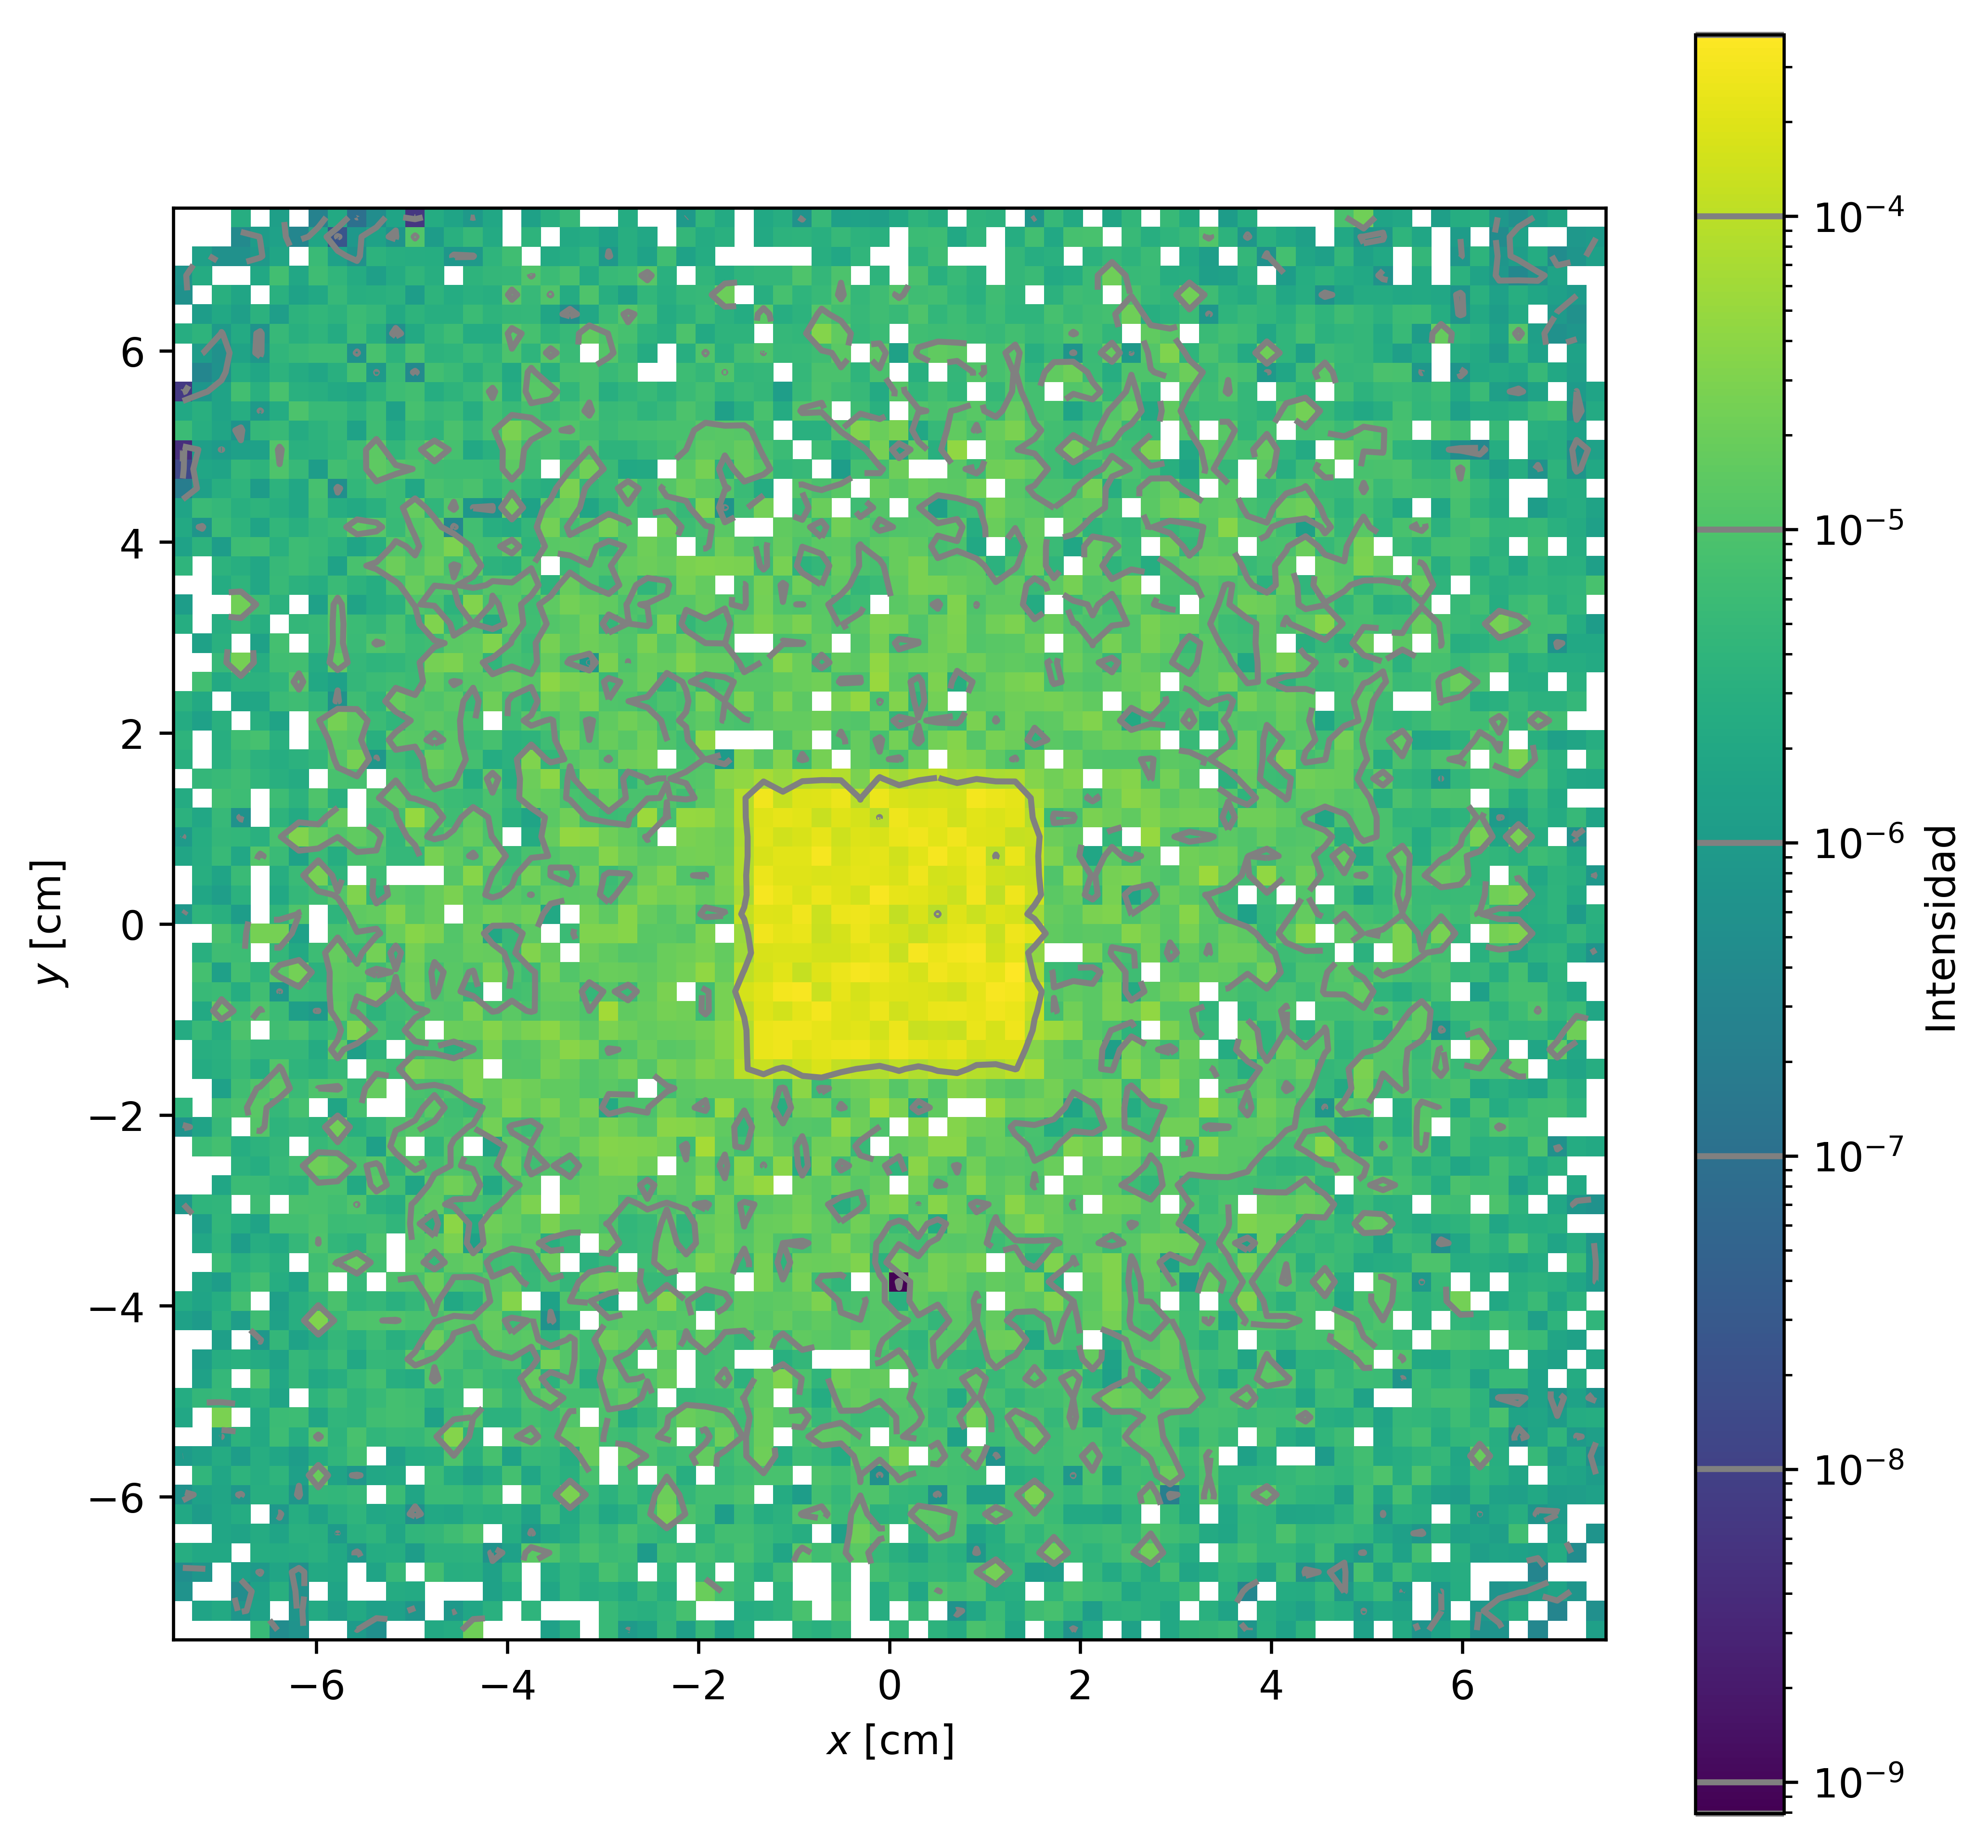
\includegraphics[width=0.75\textwidth]{figs/fig4_1.png}
    \caption{Distribución de $X$ vs $Y$ para el archivo de partículas registrado en la primera simulación del tubo de vacío.}
    \label{fig:trackfile1_x_y}
\end{figure}

Este conjunto contiene dos poblaciones de neutrones claramente diferenciadas. La primera corresponde a neutrones que no han sufrido colisiones: todos ellos presentan dirección $\mu = 1$ y una letargía fija correspondiente a una energía de $E = 1~MeV$, donde $\textit{letargía} = ln(E_0/E)$ con $E_0 = 20~MeV$. Estos valores coinciden con la configuración de la fuente original, la cual fue definida como perfectamente colimada y monoenergética. La segunda población está compuesta por neutrones que han interactuado con el medio: en este caso, las distribuciones de $\mu$ y letargía se extienden de forma continua, reflejando los efectos introducidos por las colisiones. Este comportamiento se observa en la Figura\ref{fig:trackfile1_letargia_mu}, donde se presentan las distribuciones de letargía y $\mu$ correspondientes al archivo de partículas registrado en la primera simulación del tubo de vacío.

Este conjunto contiene dos poblaciones de neutrones claramente diferenciadas. La primera corresponde a neutrones que no han sufrido colisiones: todos ellos poseen dirección $\mu = 1$ y una letargía fija, correspondiente a $E = 1~MeV$, sin dispersión alguna, lo cual concuerda con que la fuente original fue configurada con estos valores de forma determinista. La segunda población incluye neutrones que han colisionado: en este caso, las distribuciones de $\mu$ y letargía son más amplias y continuas, reflejando la dispersión introducida por las interacciones. Este comportamiento se observa en la Figura \ref{fig:trackfile1_letargia_mu}, donde se presentan las distribuciones de letargía y $\mu$ para el archivo de partículas registrado en la primera simulación del tubo de vacío. 

\begin{figure}[H]
    \centering
    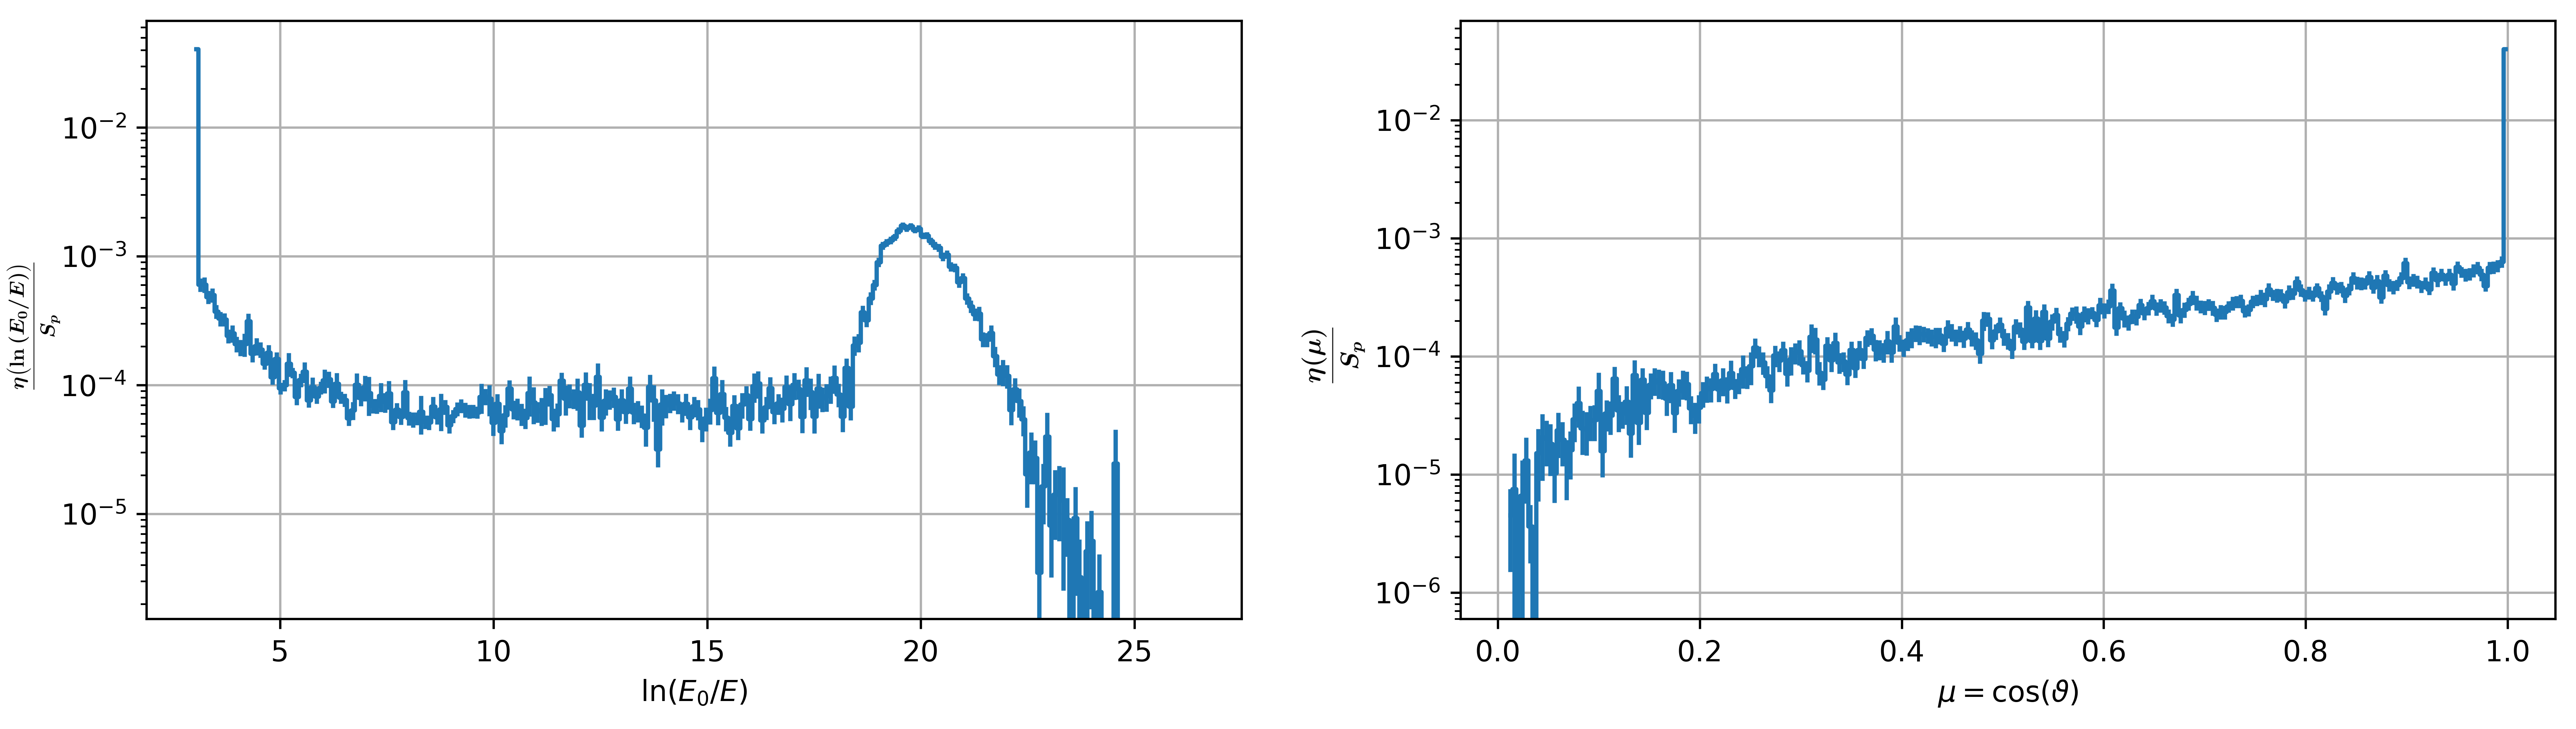
\includegraphics[width=\textwidth]{figs/fig4_2.png}
    \caption{Distribuciones de letargía y $\mu$ para el archivo de partículas registrado en la primera simulación del tubo de vacío, con escala logarítmica en el eje y. Se observa la presencia de dos poblaciones: una concentrada en $\mu = 1$ y letargía fija correspondiente a una energía de $E = 1~MeV$, montada sobre una distribución continua de neutrones colisionados.}
    \label{fig:trackfile1_letargia_mu}
\end{figure}

Esta doble estructura se evidencia particularmente en los gráficos bidimensionales de letargía vs. $\mu$, donde ambas poblaciones aparecen como conjuntos diferenciados. Tal como se muestra en la Figura \ref{fig:trackfile1_letargia_mu_2}, los neutrones no colisionados se concentran en un único punto en $\mu = 1$ y letargía fija correspondiente a una energía de $E = 1~MeV$, mientras que los neutrones colisionados forman una distribución extendida continua, con un agrupamiento en la región de termalización. Este fenómeno plantea un desafío para los métodos de muestreo, al requerir una representación precisa tanto de distribuciones tipo delta como de distribuciones extendidas.


Tanto en la Figura~\ref{fig:trackfile1_x_y} como en la Figura~\ref{fig:trackfile1_letargia_mu_2} puede observarse que existen regiones del espacio de fases donde no se registran neutrones. Esto se debe a que el archivo de partículas original contiene una cantidad finita de neutrones, lo que limita la cobertura en determinadas regiones del espacio de fases. El objetivo del método propuesto consiste en remuestrear dicho archivo original para generar un nuevo conjunto de partículas que preserve las correlaciones presentes, pero que a su vez mejore la estadística en aquellas regiones originalmente poco representadas.


\begin{figure}[H]
    \centering
    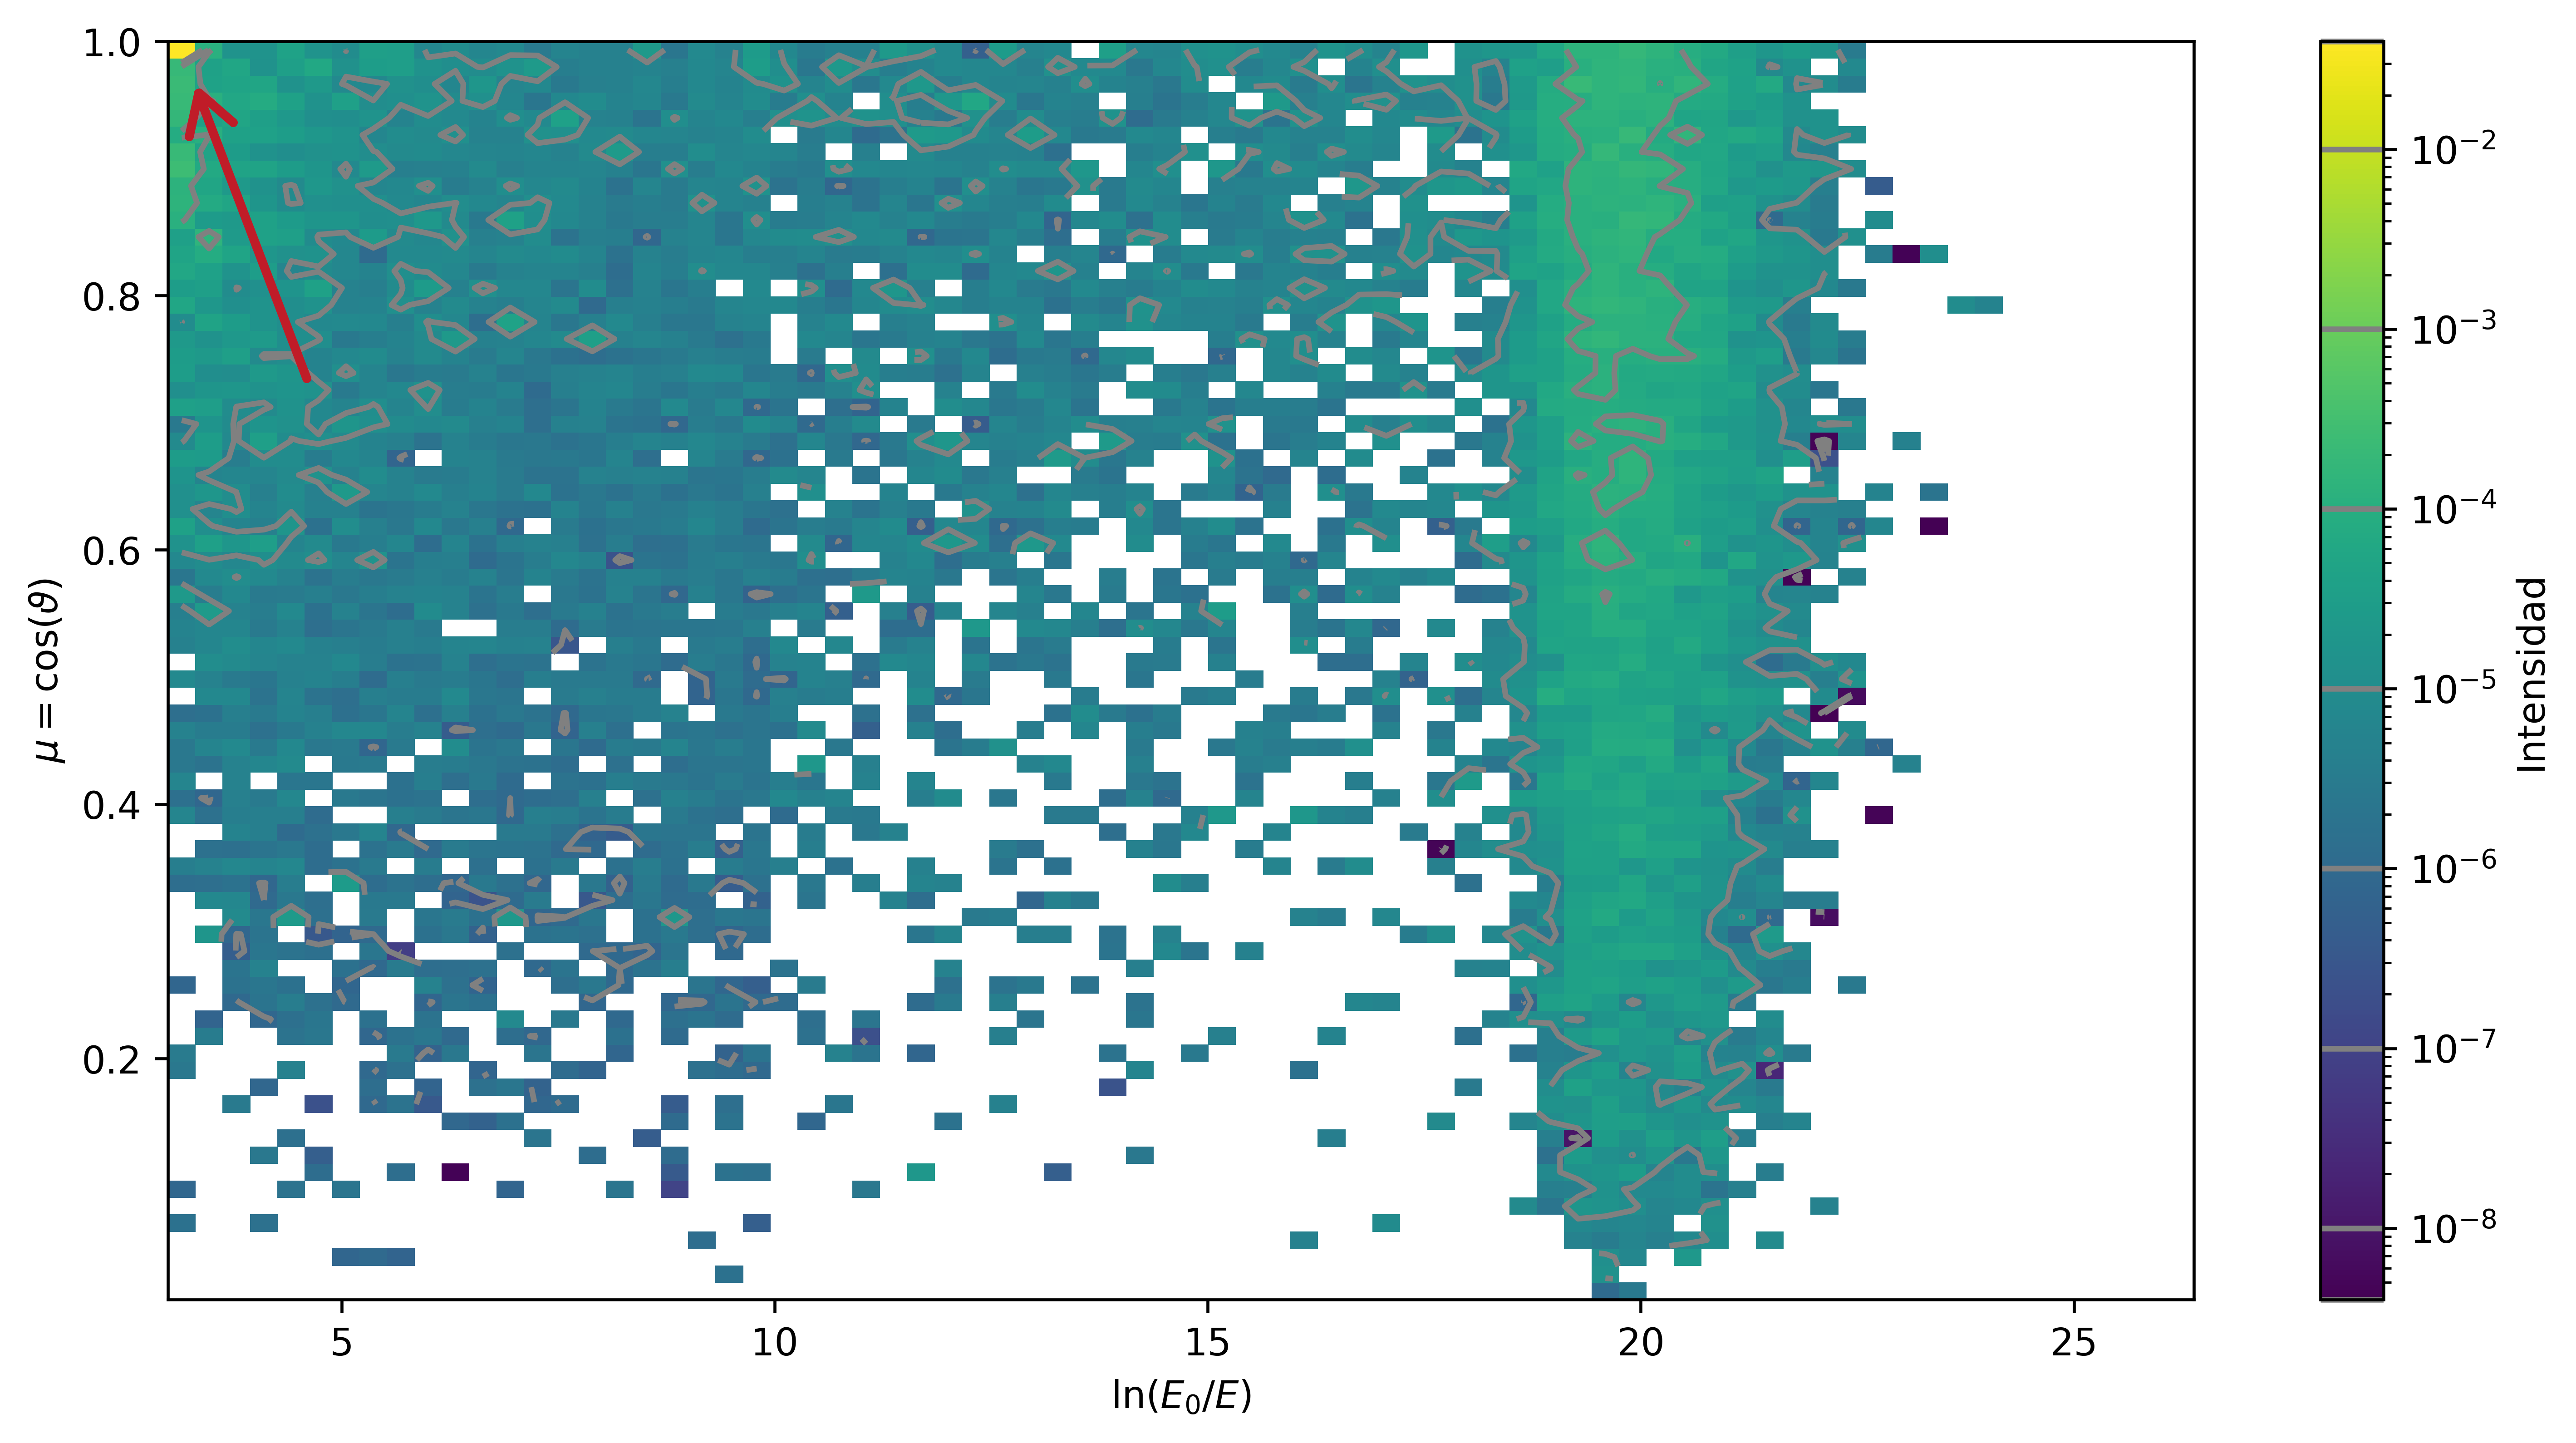
\includegraphics[width=0.9\textwidth]{figs/fig4_3.png}
    \caption{Distribuciones de letargía vs $\mu$ para el archivo de partículas original. Se observa la presencia de un conjunto de neutrones graficados como un píxel en $\mu = 1$ y letargía mínima. A su vez se observa la presencia de un segundo conjunto de neutrones colisionados, que se distribuyen en el plano de forma continua, con un agrupamiento sobre letargía = 20, indicando la termalización de los neutrones.}
    \label{fig:trackfile1_letargia_mu_2}
\end{figure}

\section{Procesamiento preliminar del archivo de partículas}
\subsection{Metodología del análisis}
\label{sec:metodologia-analisis}

El análisis realizado en este capítulo se centra en evaluar la influencia del tipo de bineado aplicado, así como la incorporación de bordes manuales en la segmentación del espacio de fases. Los tipos de bineado considerados son:
\begin{itemize}
    \item Caso 1: bineado uniforme sin bordes manuales.
    \item Caso 2: bineado uniforme con bordes definidos por el usuario.
    \item Caso 3: bineado adaptativo sin bordes manuales.
    \item Caso 4: bineado adaptativo con bordes definidos por el usuario.
\end{itemize}

Los bordes manuales son establecidos debido al conocimiento previo de la fuente utilizada para diferenciar poblaciones de neutrones. Concretamente, se incorporan bordes en la variable letargía y en la dirección cosenoidal ($\mu$) para distinguir los neutrones que no han colisionado. Adicionalmente, se incluyen bordes espaciales en las coordenadas $X$ e $Y$ para separar los neutrones que atraviesan el tubo de vacío respecto de aquellos que interactúan con el agua circundante.

Con el objetivo de realizar un análisis consistente y evitar sesgos derivados del procedimiento, se mantiene constante en todos los casos el orden de procesamiento de las variables y la configuración de los histogramas. Esta etapa preliminar permite una comparación entre los cuatro métodos de bineado evaluados en esta sección. El orden seleccionado para el procesamiento es \texttt{[letargía, X, Y, $\mu$, $\phi$]}. Esta elección responde a que al inicio del procesamiento, la discretización se aplica sobre el conjunto completo de partículas, mientras que las variables procesadas posteriormente actúan sobre subconjuntos cada vez más reducidos. Por este motivo, se eligió comenzar con la letargía para priorizar describir el comportamiento espectral. A continuación se aplican las variables espaciales (\texttt{X} e \texttt{Y}), con el fin de preservar correctamente la ubicación de las partículas en regiones geométricamente diferenciadas (vacío o agua). Finalmente, se dejó para el último lugar la variable \texttt{$\phi$}, cuya distribución se espera relativamente uniforme, por lo que no requiere un nivel de detalle elevado.

Asimismo, se conservan fijos los números de bines utilizados en los histogramas macro y micro: se emplean \texttt{[5, 5, 5, 5]} bines para los macrogrupos y \texttt{[36, 36, 36, 36, 36]} para los microgrupos, respectivamente. Esta configuración constante garantiza que las comparaciones entre métodos se basen únicamente en el esquema de discretizacion utilizado y no en diferencias en la resolución.

Posteriormente, el análisis se estructura en tres partes:

\begin{itemize}
\item \textbf{Distribuciones de letargía:} se presentan y comparan las distribuciones de letargía obtenidas para cada uno de los cuatro esquemas evaluados, comparándolas contra la distribución registrada en el archivo original.
\item \textbf{Distribuciones de $\mu$:} se analizan de forma análoga las distribuciones de la variable direccional $\mu = \cos\theta$, evaluando en qué medida se preserva la estructura angular del haz en cada uno de los casos.

\item \textbf{Distribuciones espaciales $X$–$Y$:} se analizan los resultados mediante mapas bidimensionales para cada una de las configuraciones, comparando las distribuciones generadas contra las distribuciones originales.
\end{itemize}

\subsection{Distribuciones de letargía}
A continuación se analizan las distribuciones remuestreadas de letargía obtenidas mediante los 4 casos de configuración analizados.

En la Figura \ref{fig:let_1}, correspondiente al caso 1 de bineado uniforme sin bordes, se observa que esta configuración presenta limitaciones en regiones de alta densidad estadística. En particular, la delta en la zona de letargía correspondiente a una energía de $E = 1~MeV$ —asociada a neutrones no colisionados— es reemplazada por un escalón con el ancho del bin, perdiéndose el comportamiento tipo delta. Asimismo, en la región de termalización, la resolución es insuficiente para capturar adecuadamente los cambios de forma.

\begin{figure}[H]
    \centering
    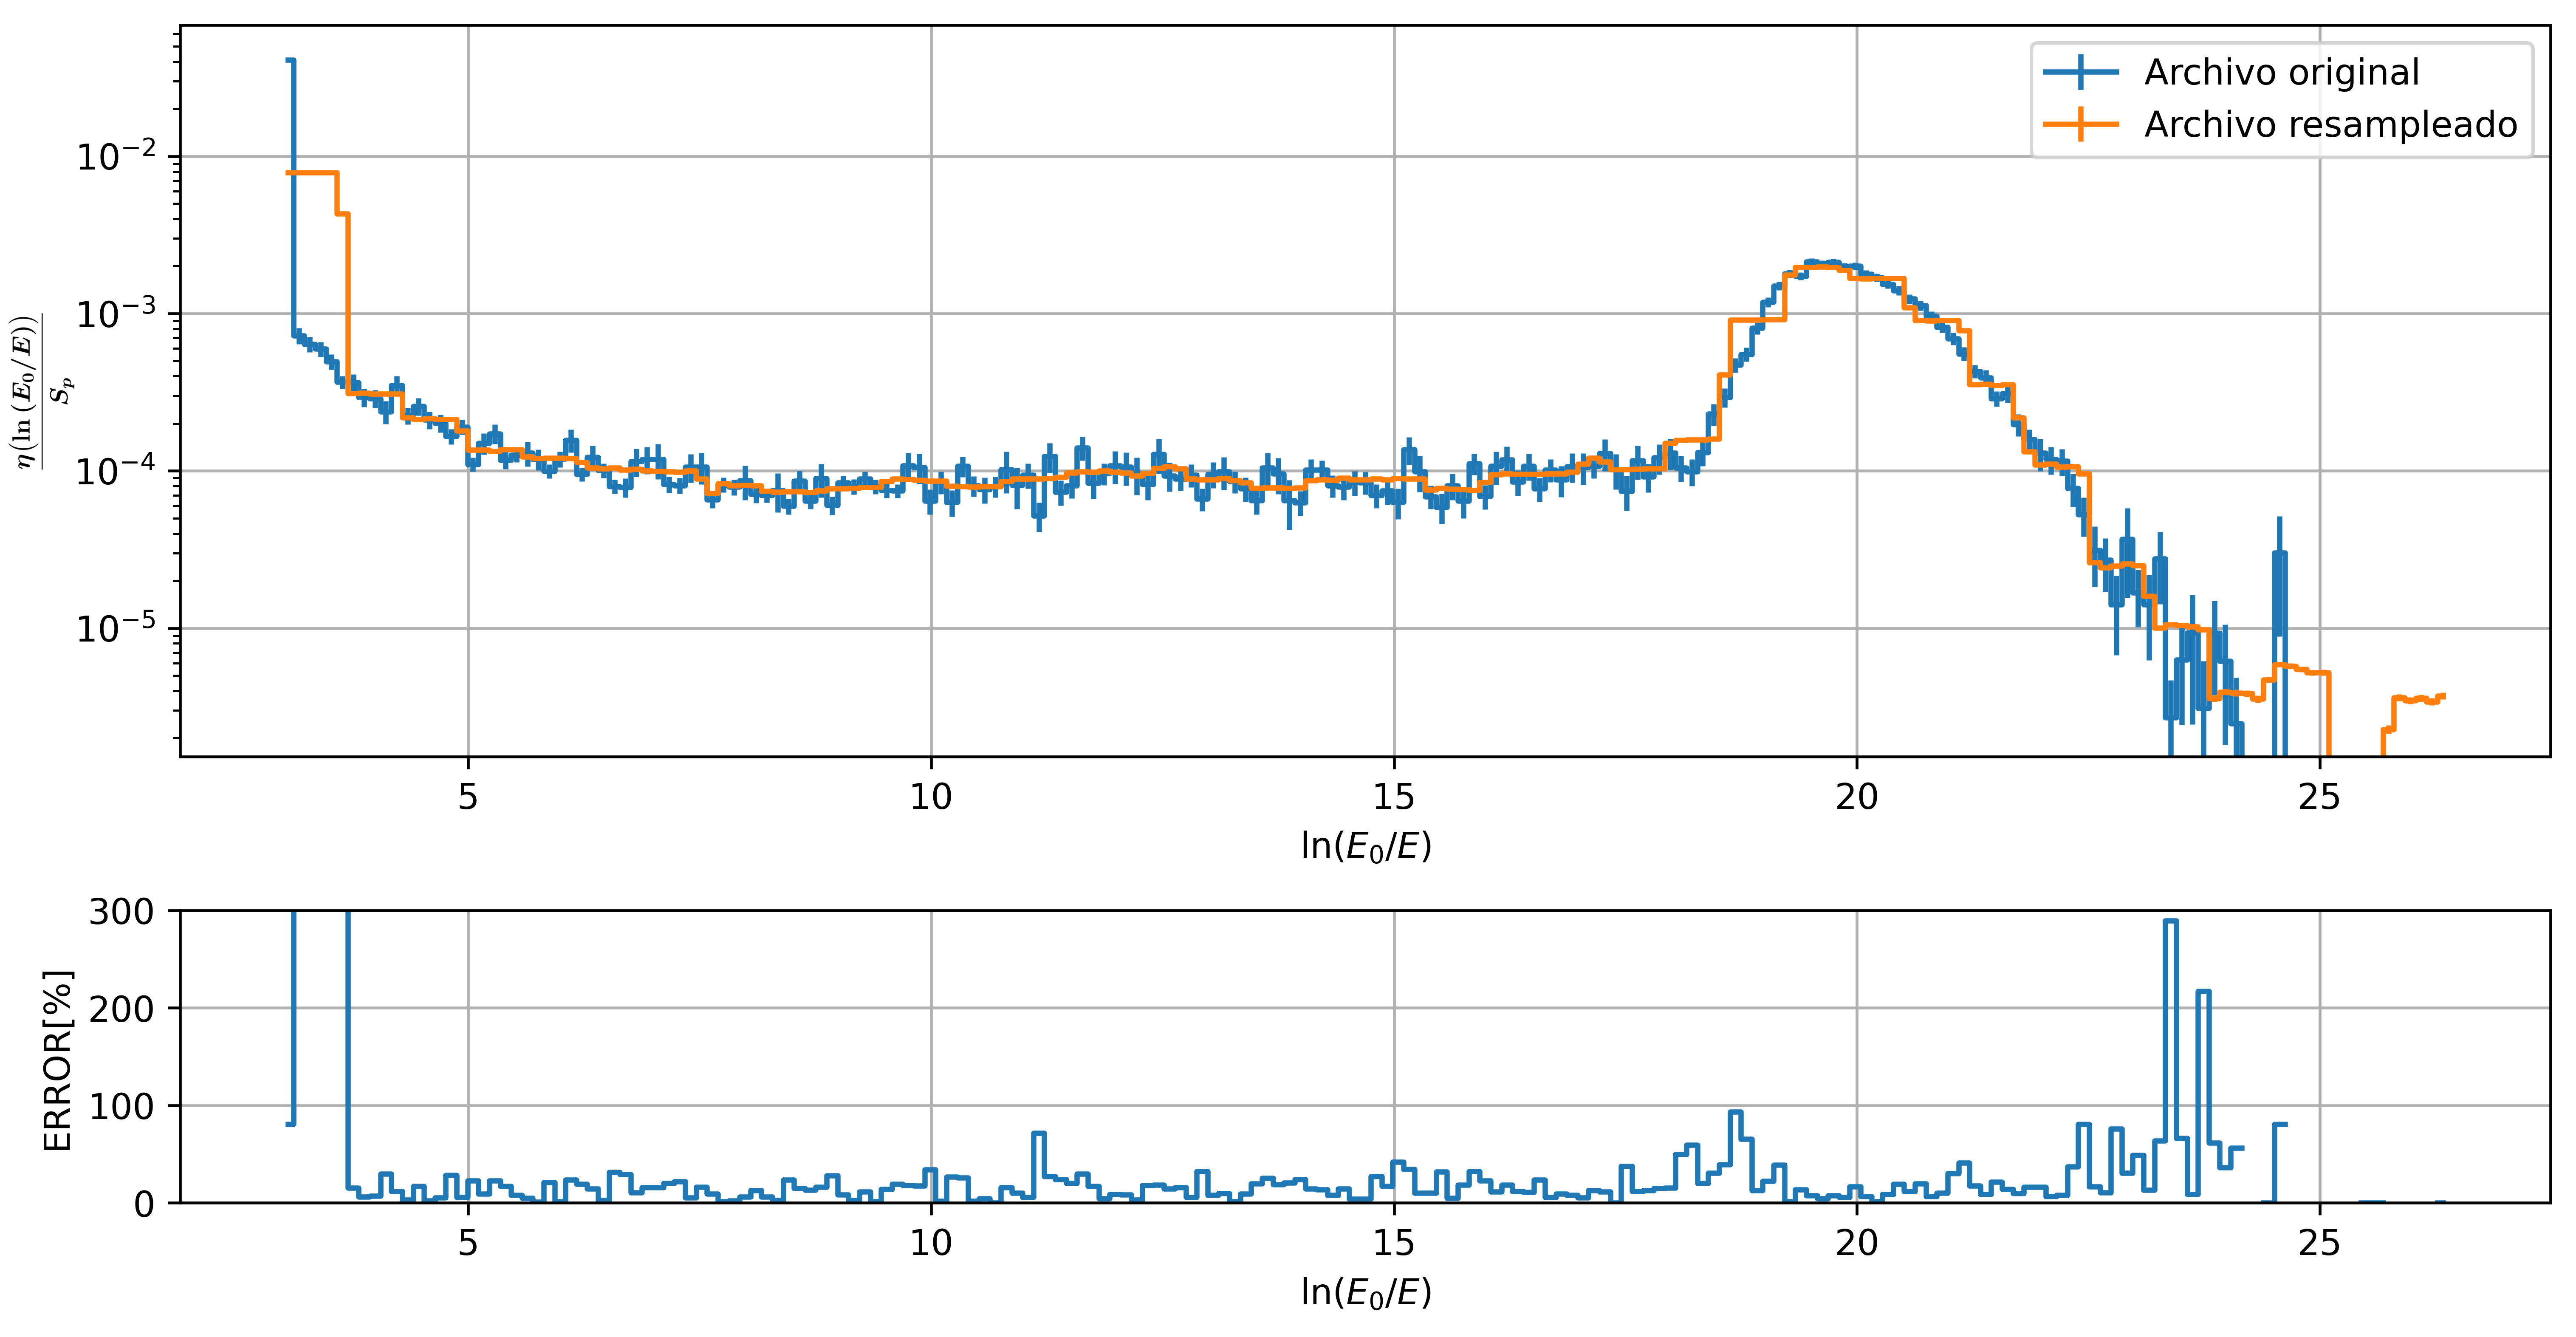
\includegraphics[width=\textwidth]{let_1.png}
    \caption{Distribución remuestreada de letargía para el caso de bineado uniforme sin bordes manuales.}
    \label{fig:let_1}
\end{figure}

La Figura \ref{fig:let_2} muestra el caso 2 en el que se introduce un borde manual para separar la letargía correspondiente a una energía de $E = 1~MeV$. Esta intervención permite mejorar la representación de la delta, capturando con mayor fidelidad los neutrones no colisionados. Sin embargo, el resto de la distribución sigue estando limitada por la resolución uniforme, en particular en la zona de termalización.

En la Figura \ref{fig:let_3}, se presenta el resultado del caso 3 utilizando histogramas adaptativos sin bordes manuales. Este método asigna una mayor densidad de bines en zonas con mayor estadística, lo que permite una mejor representación tanto de la delta en letargía correspondiente a una energía de $E = 1~MeV$ como de la región de termalización. Se observa un seguimiento más suave y detallado de la distribución, y una reducción del error relativo en las zonas relevantes.

\begin{figure}[H]
    \centering
    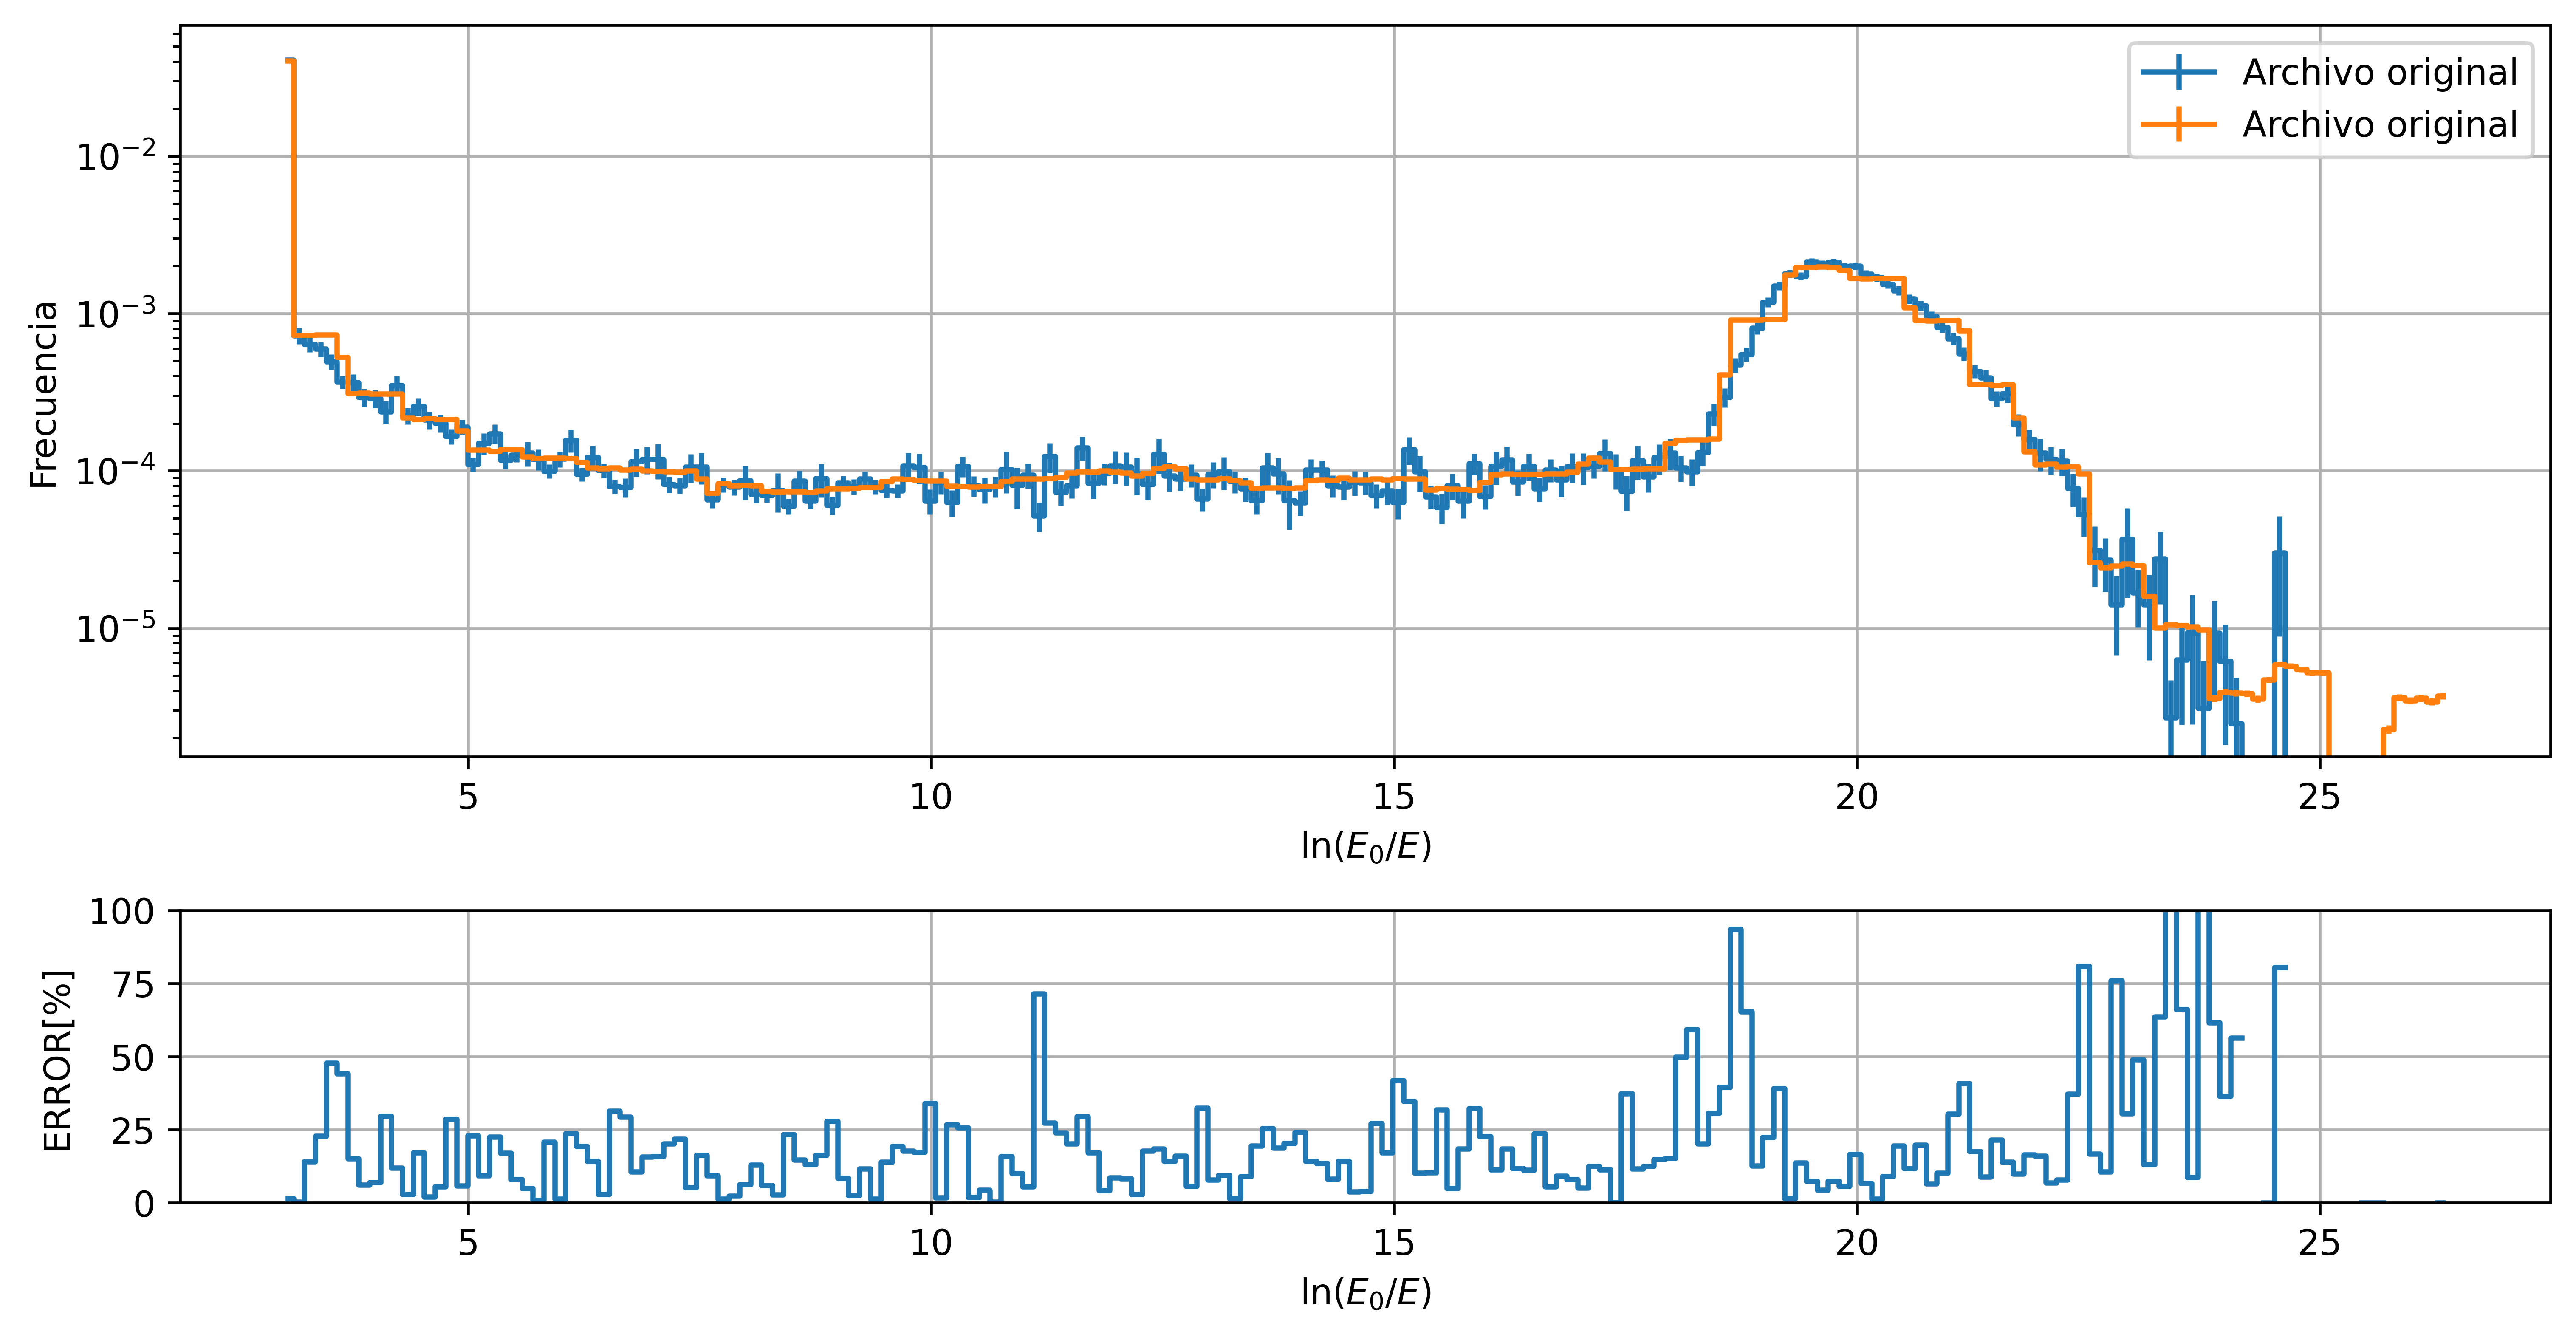
\includegraphics[width=\textwidth]{let_2.png}
    \caption{Distribución remuestreada de letargía para el caso de bineado uniforme con borde manual en la zona de letargía correspondiente a una energía de $E = 1~MeV$.}
    \label{fig:let_2}
\end{figure}

Finalmente, en la Figura \ref{fig:let_4}, se muestra el resultado del caso 4 con el método adaptativo con bordes manuales. No se observan diferencias significativas con respecto al caso sin bordes, lo que demuestra que el algoritmo es capaz de identificar y segmentar eficientemente las zonas relevantes de forma autónoma, incluso sin información previa de la fuente brindada por el borde manual.

\begin{figure}[H]
    \centering
    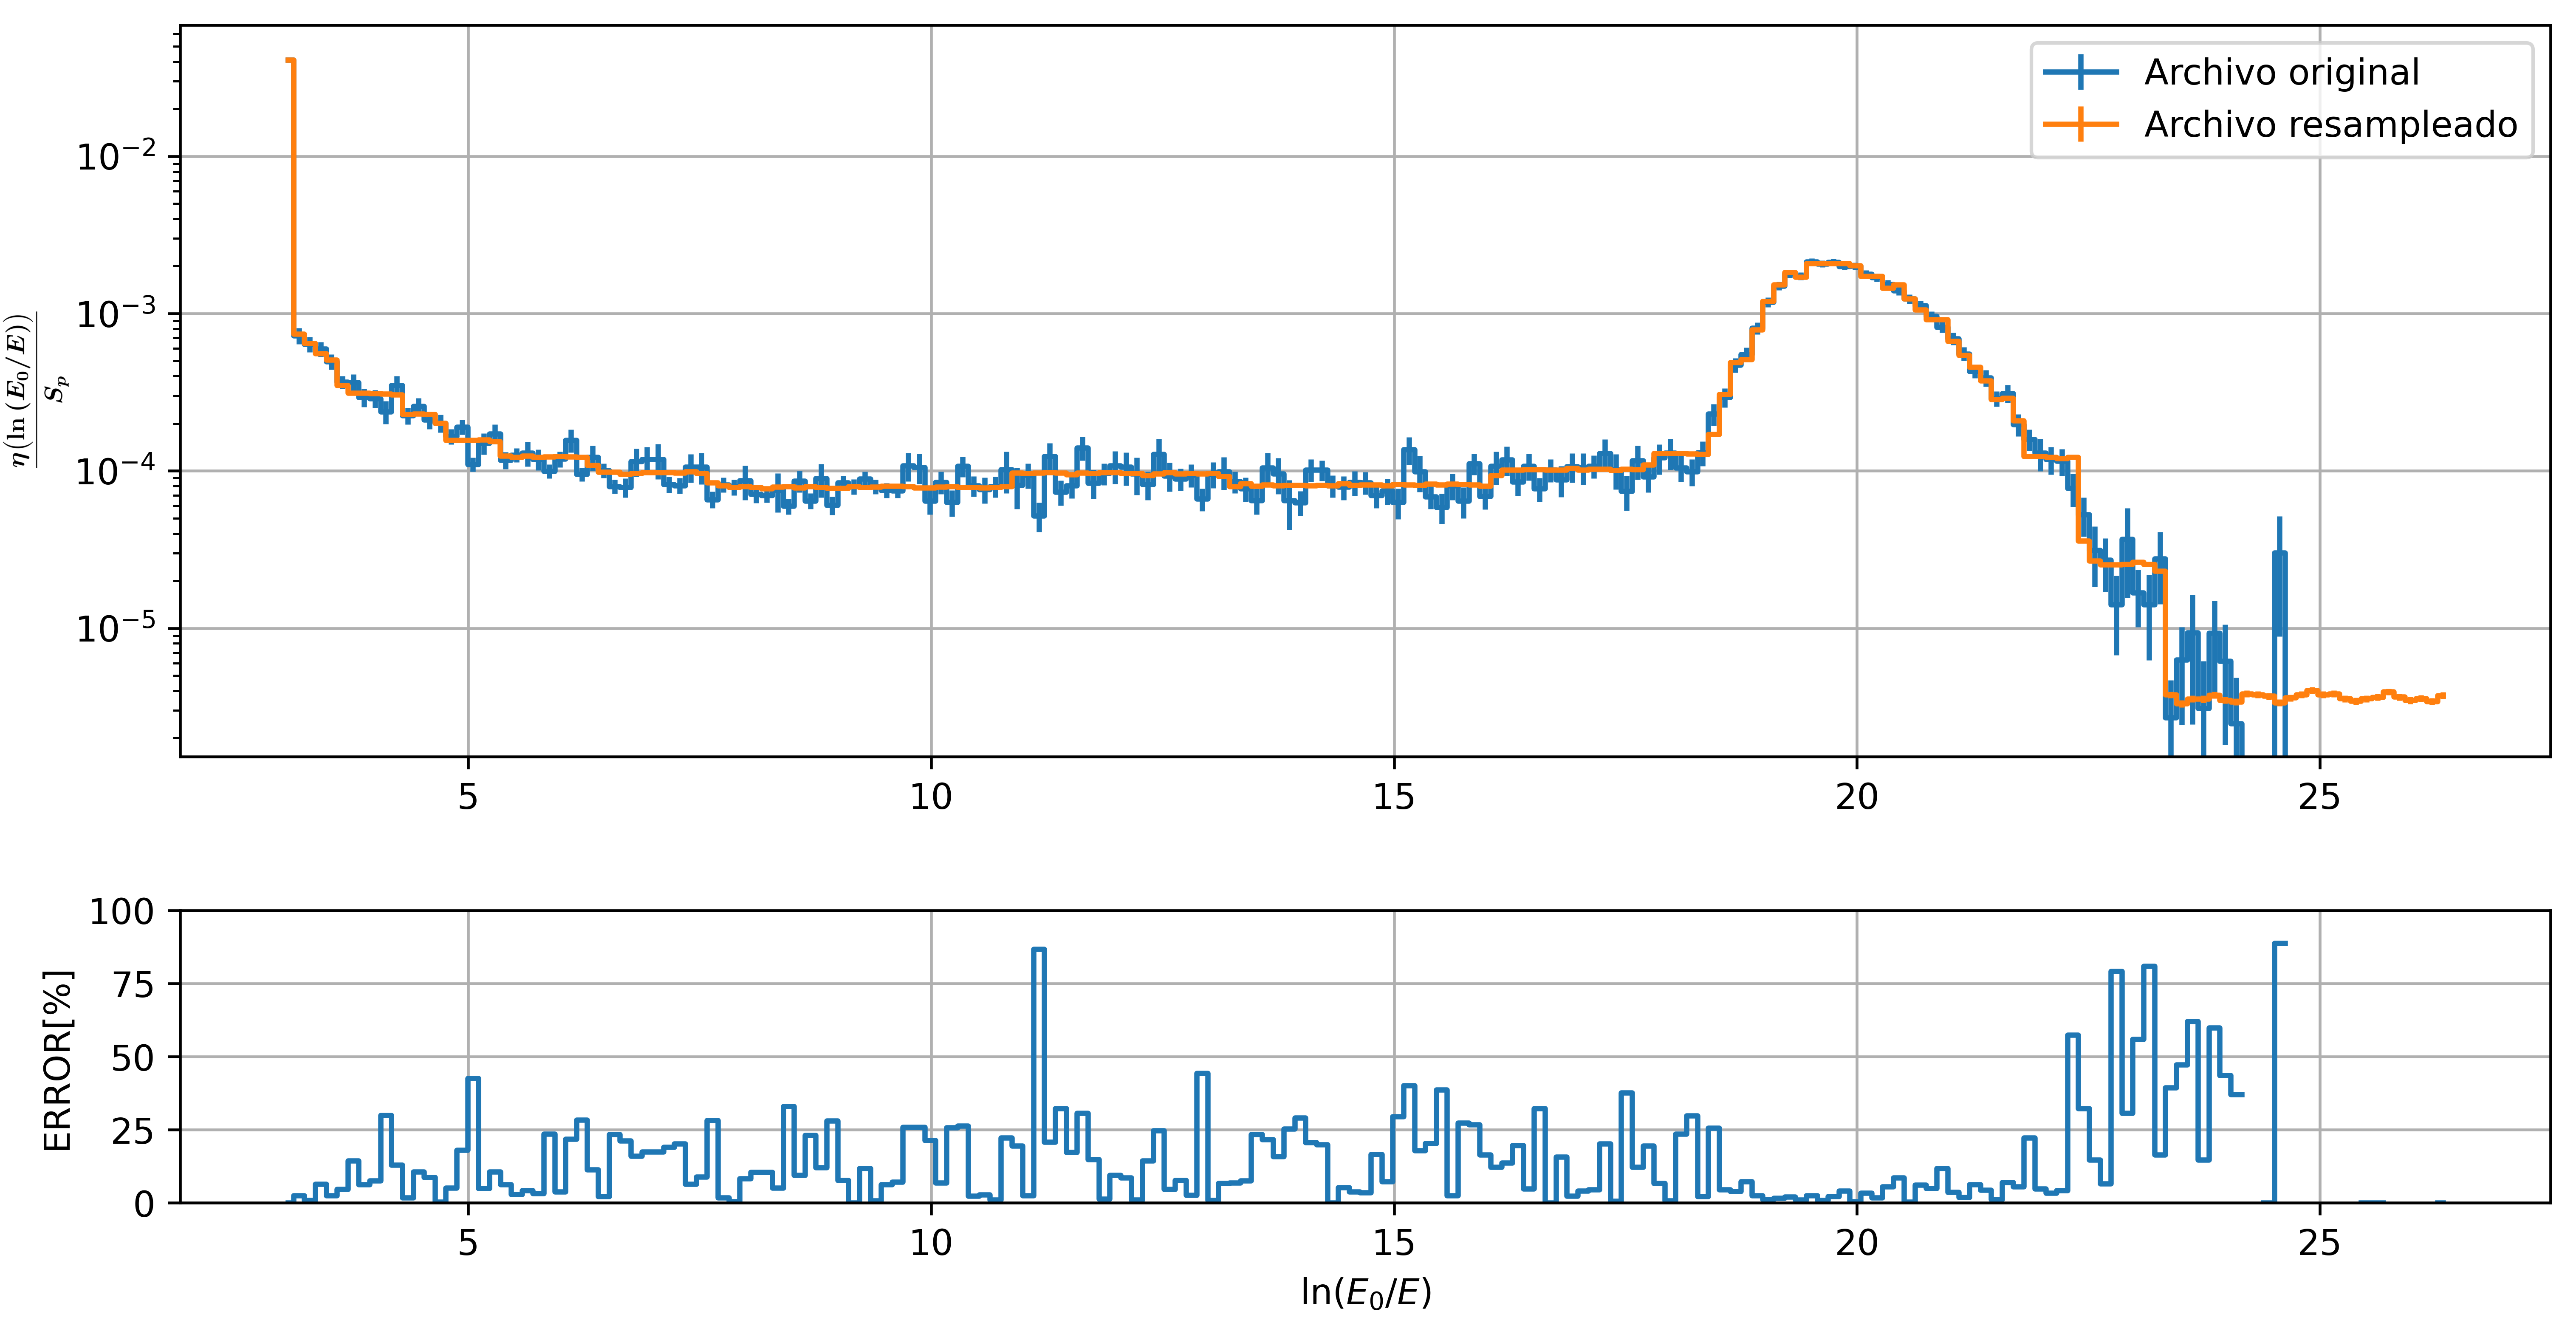
\includegraphics[width=\textwidth]{let_3.png}
    \caption{Distribución remuestreada de letargía para el caso de bineado adaptativo sin bordes manuales.}
    \label{fig:let_3}
\end{figure}

\begin{figure}[H]
    \centering
    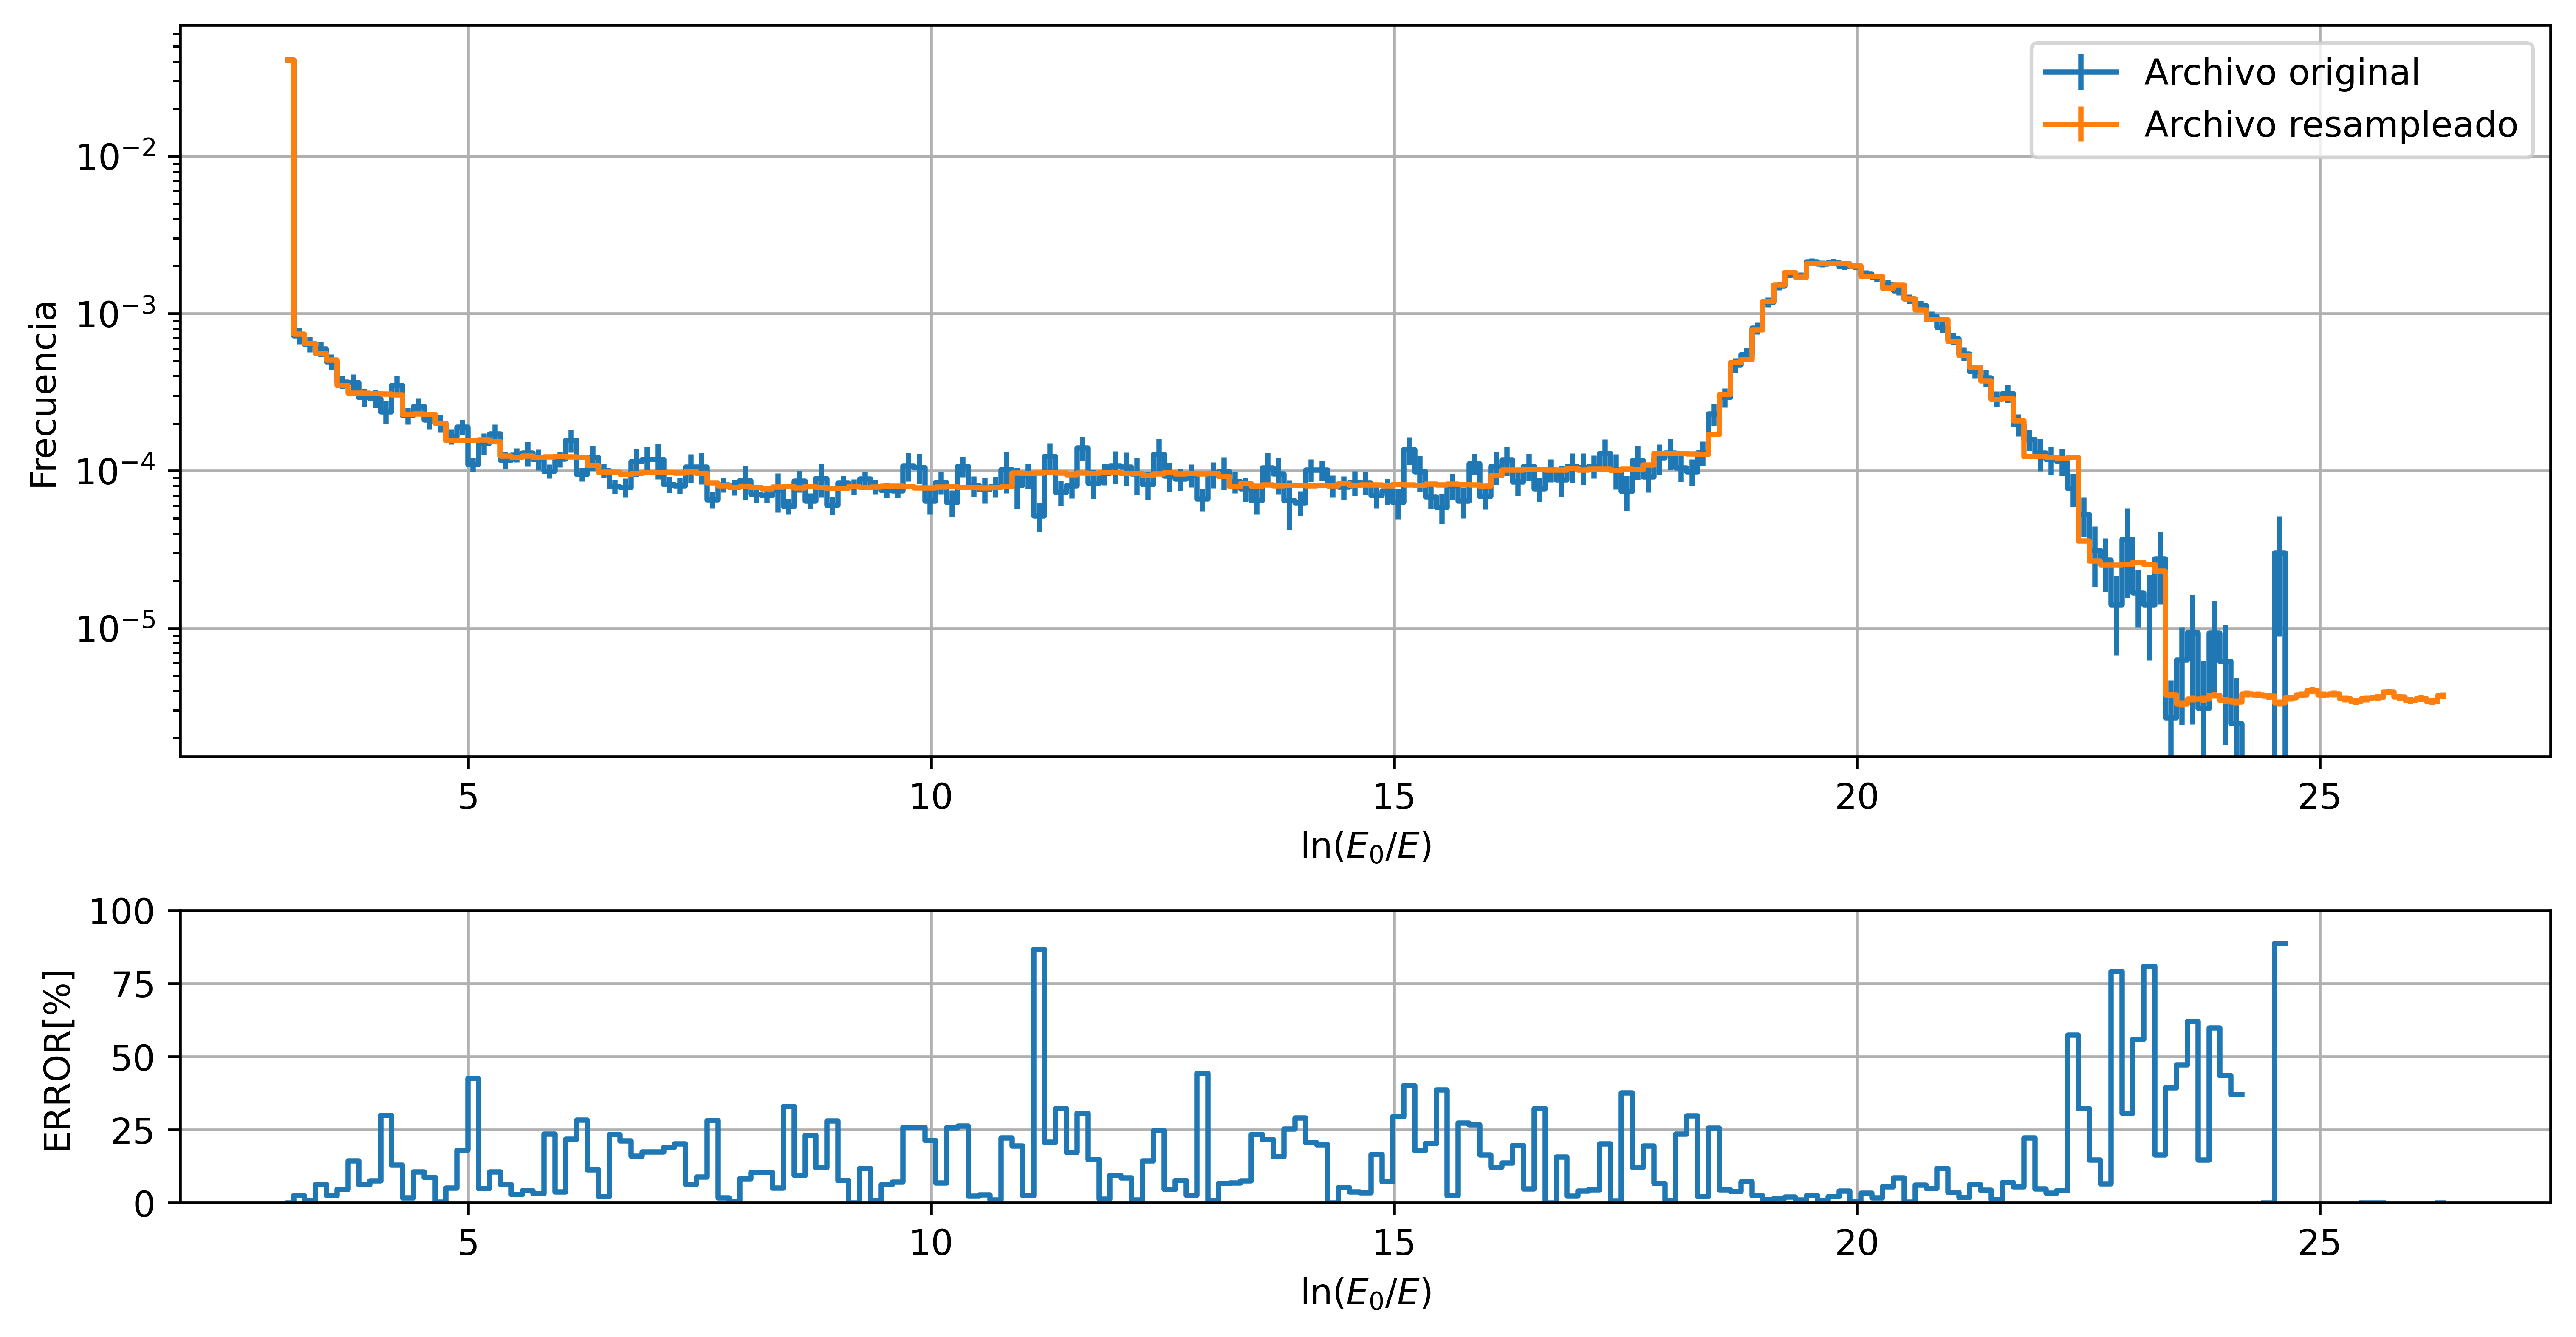
\includegraphics[width=\textwidth]{let_4.png}
    \caption{Distribución remuestreada de letargía para el caso de bineado adaptativo con borde manual en la zona de letargía correspondiente a una energía de $E = 1~MeV$.}
    \label{fig:let_4}
\end{figure}

\subsection{Distribuciones de $\mu$}
Se analizan a continuación las distribuciones remuestreadas de la variable direccional $\mu = \cos(\theta)$, obtenidas mediante las 4 configuraciones analizadas. Se evalúa la capacidad de cada método para representar adecuadamente la delta asociada a partículas colimadas ($\mu = 1$) y el comportamiento general de la distribución.

En la Figura \ref{fig:mu_1}, correspondiente al caso 1 de bineado uniforme sin bordes manuales, se observa que la delta en $\mu = 1$ es reemplazada por un escalón, debido a que el bin abarca toda la región colimada. Este efecto deteriora significativamente la representación en esa zona. Sin embargo, el resto de la distribución es tratada de forma aceptable, suavizando la distribución.

En la Figura \ref{fig:mu_2}, se introduce un borde manual para formar un bin de ancho $10^{-9}$ en la zona de $\mu = 1$, lo que permite aislar correctamente la región colimada. Como resultado, se recupera la forma tipo delta en esa zona, y se mantiene una buena representación en el resto de la distribución.

\begin{figure}[H]
    \centering
    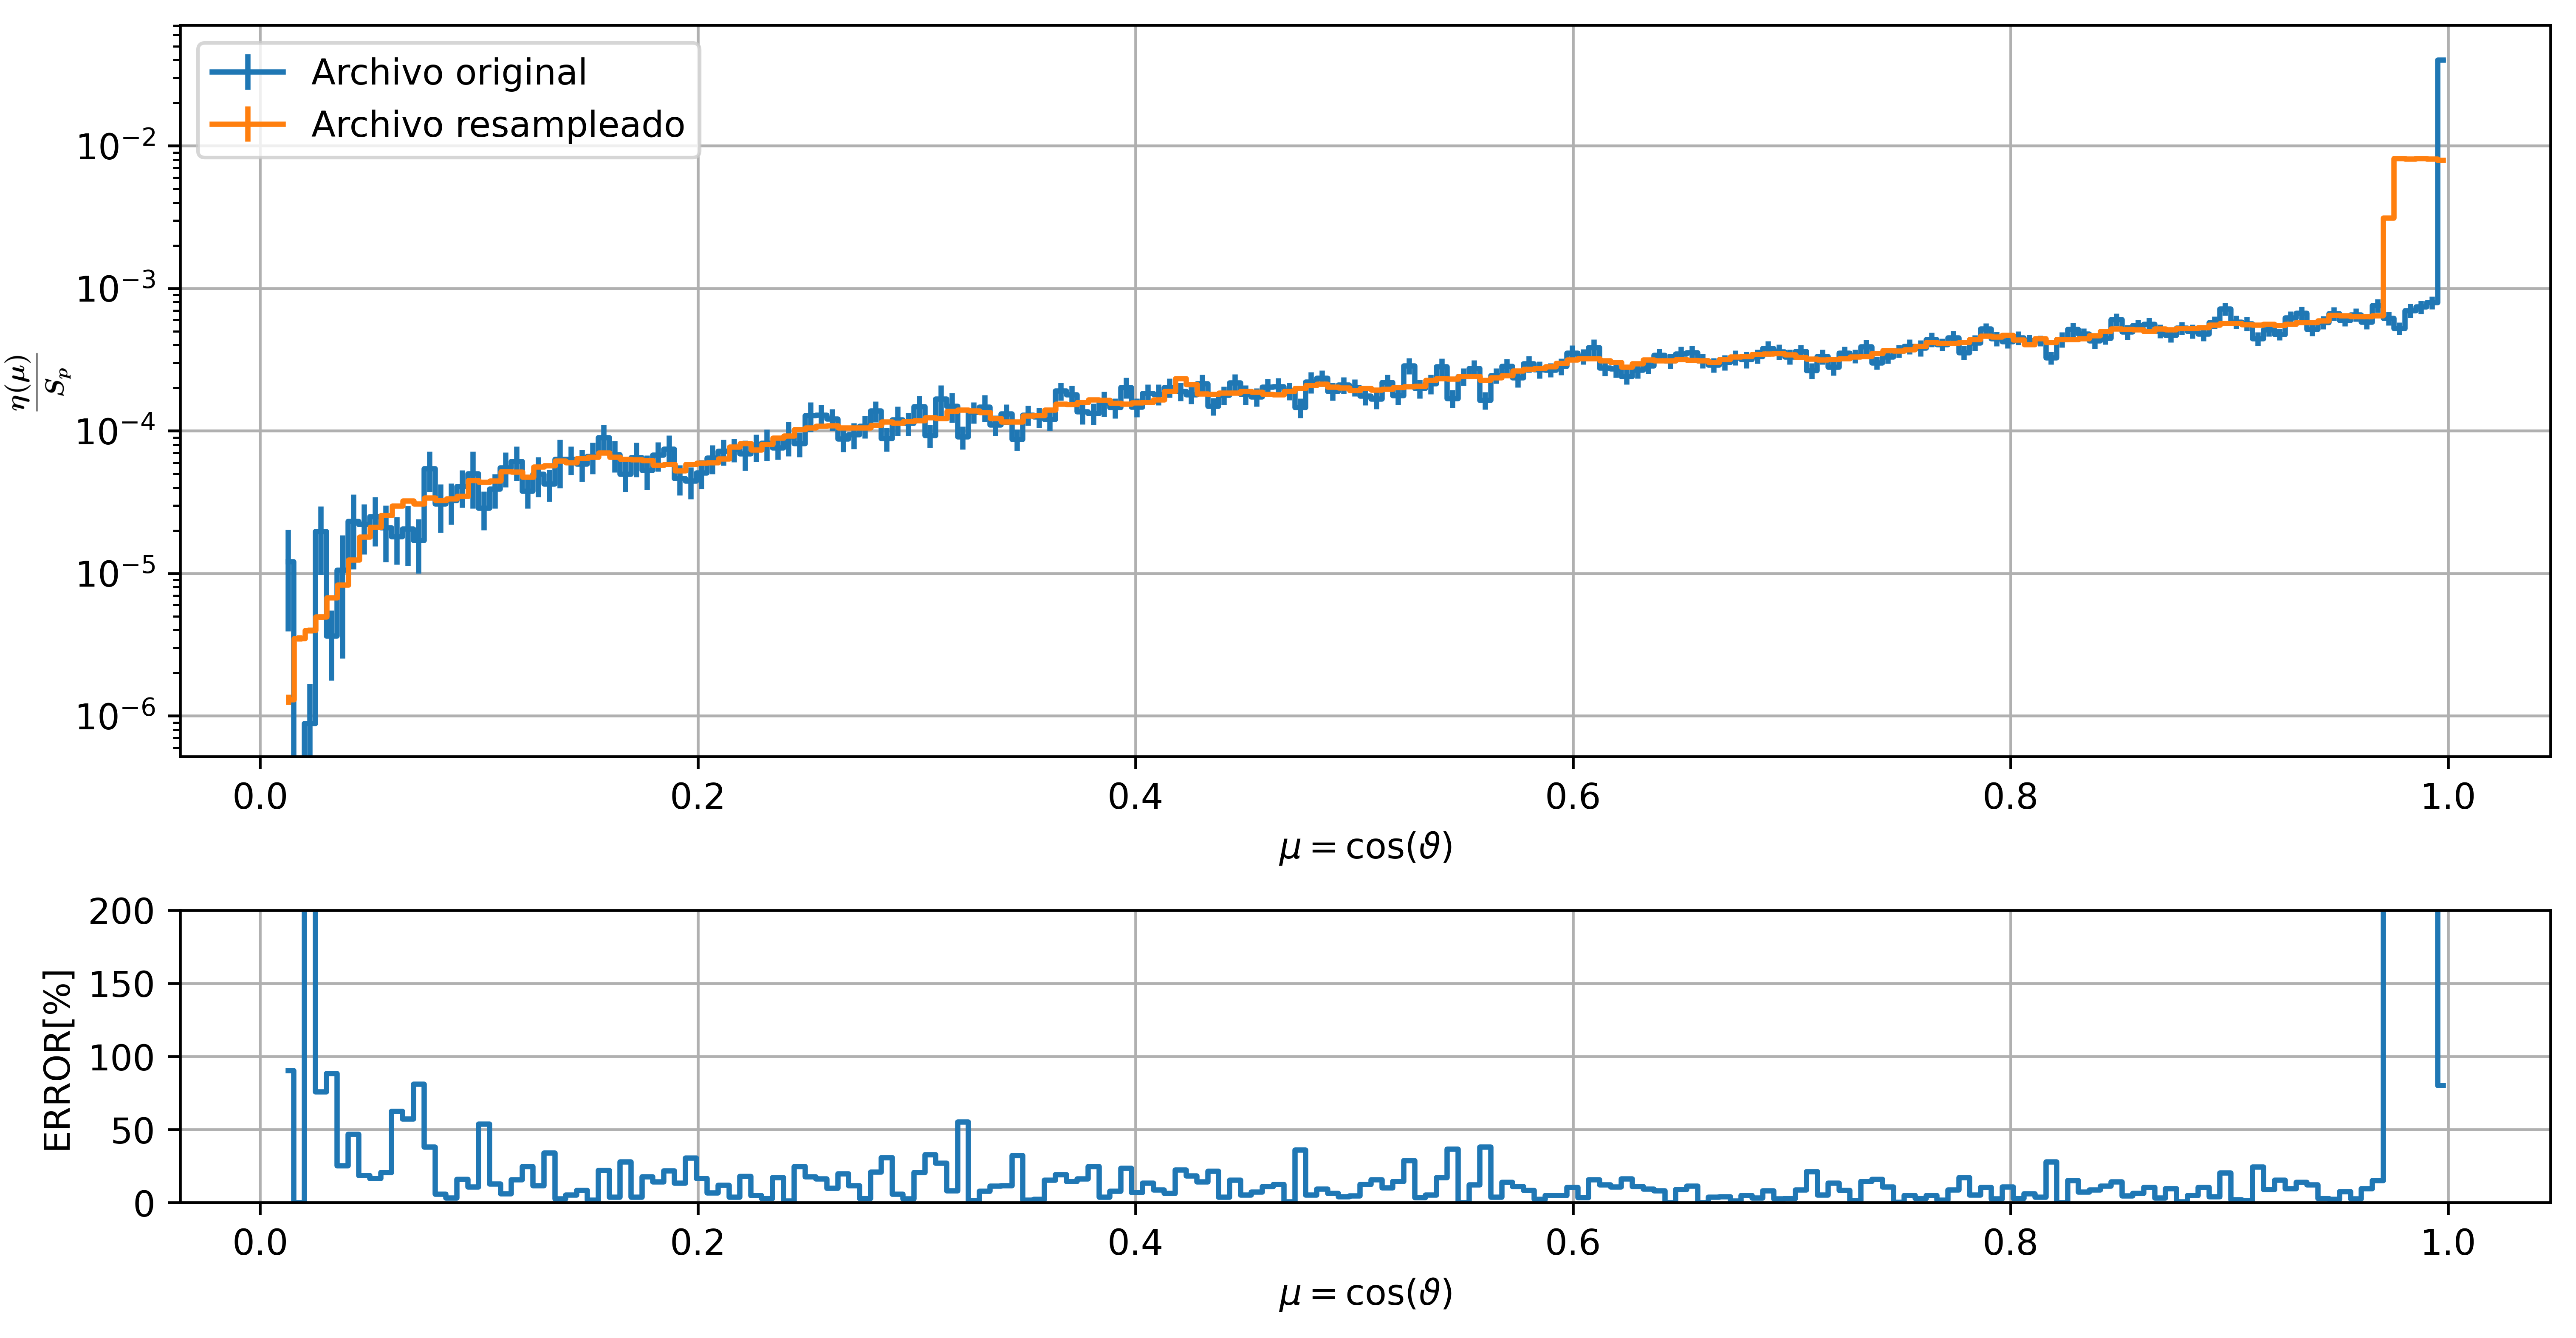
\includegraphics[width=\textwidth]{mu_1.png}
    \caption{Distribución remuestreada de $\mu$ para el caso 1 de bineado uniforme sin bordes manuales.}
    \label{fig:mu_1}
\end{figure}

\begin{figure}[H]
    \centering
    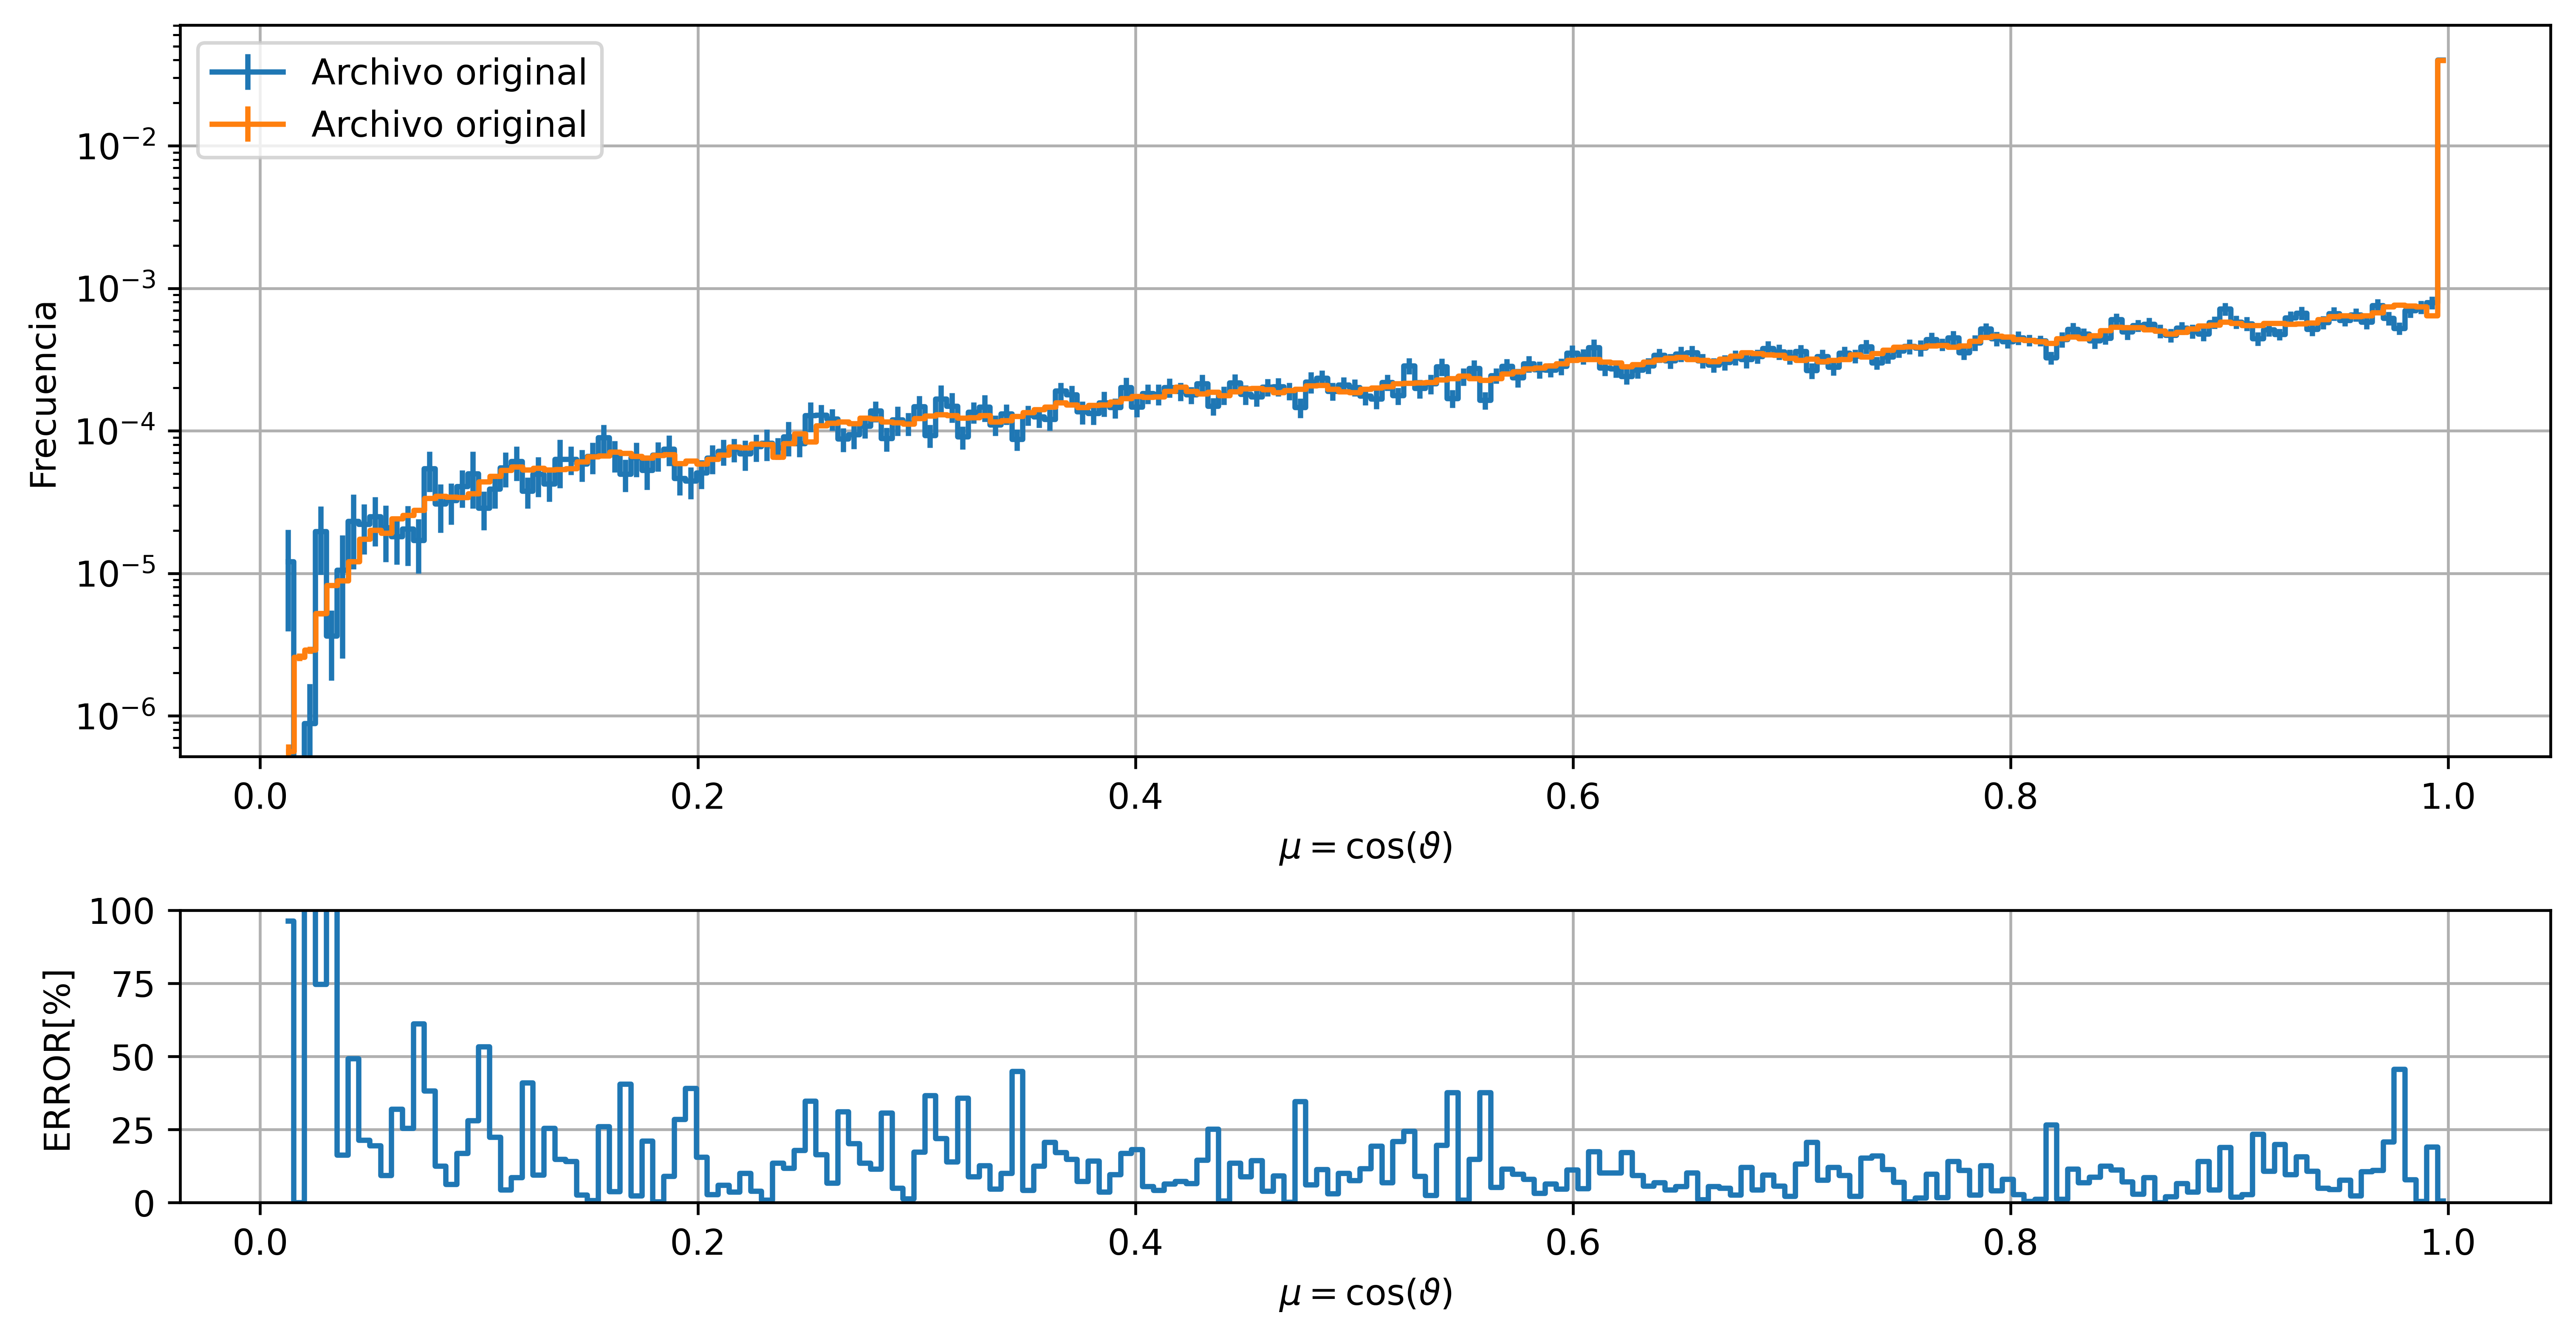
\includegraphics[width=\textwidth]{mu_2.png}
    \caption{Distribución remuestreada de $\mu$ para el caso 2 de bineado uniforme con borde manual en $\mu \approx 1$.}
    \label{fig:mu_2}
\end{figure}

La Figura \ref{fig:mu_3} muestra los resultados del caso 3 obtenidos con histogramas adaptativos sin bordes manuales. En este caso, el método logra seguir de manera precisa la forma original, tanto en la delta como en el resto de la distribución. Sin embargo, este seguimiento resulta excesivo, reproduciendo el ruido estadístico del archivo de partículas original, lo cual no es deseable. Este efecto se debe a la elevada cantidad de bines asignados: como $\mu$ es la cuarta variable en el orden de segmentación, se trabaja sobre subconjuntos reducidos de partículas, lo cual hace que 36 bines resulte una resolución desproporcionada.

\begin{figure}[H]
    \centering
    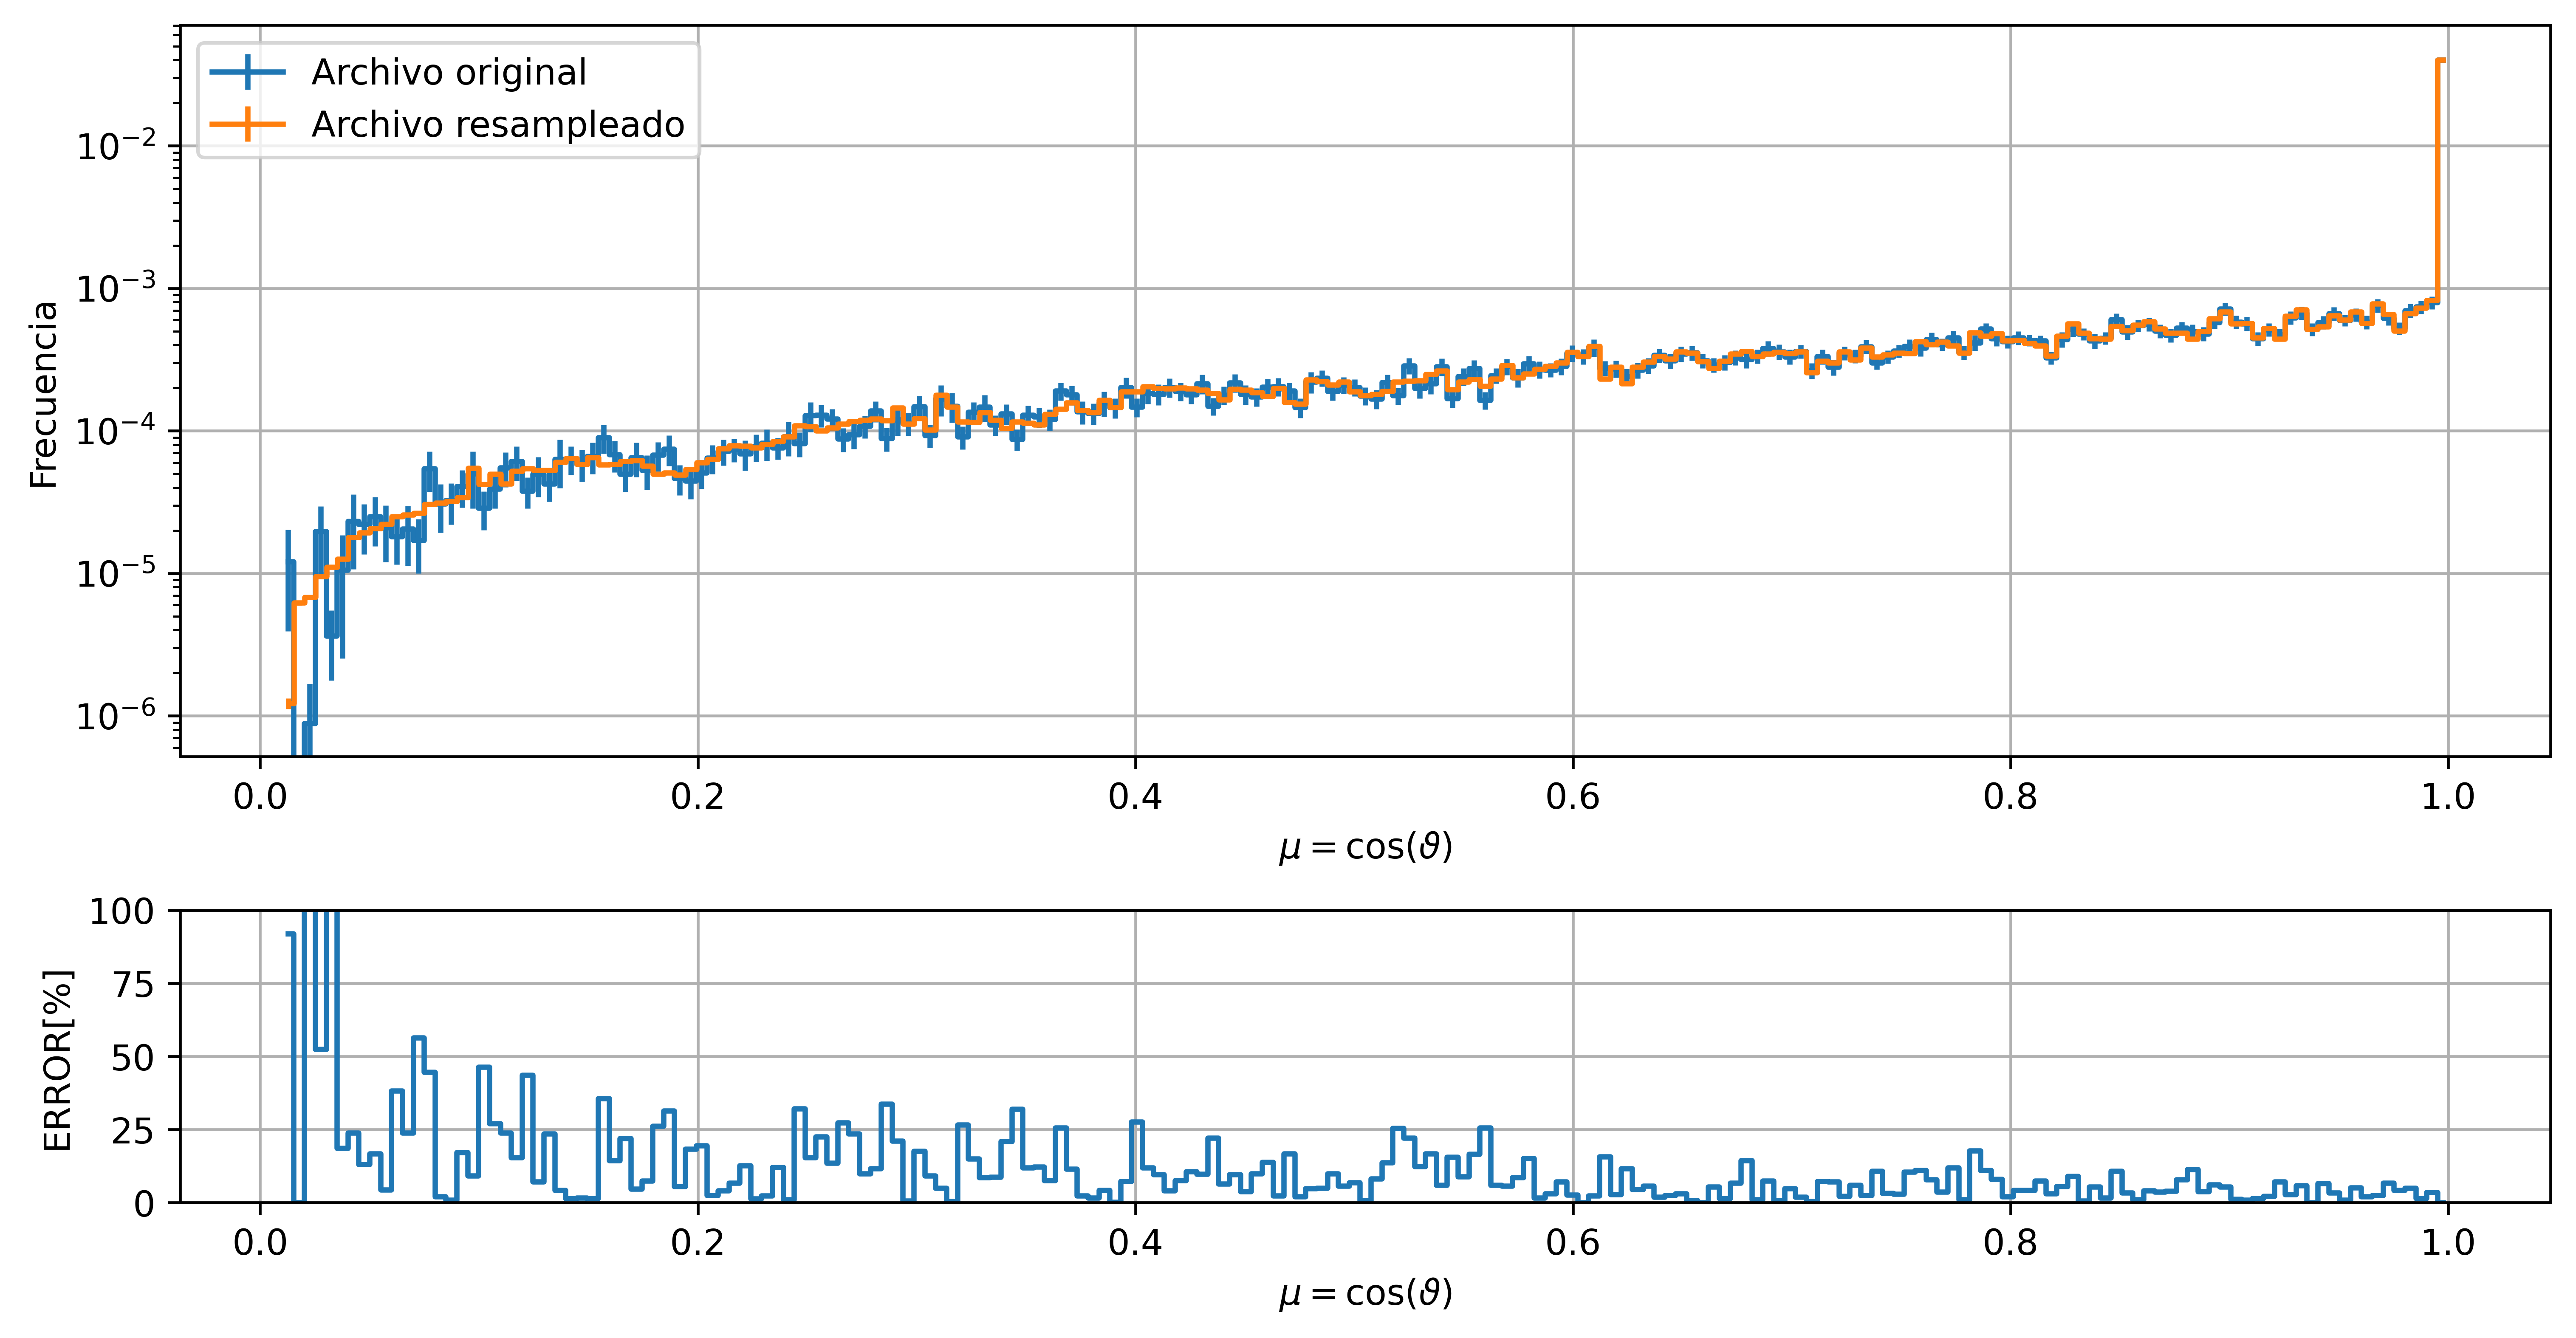
\includegraphics[width=\textwidth]{mu_3.png}
    \caption{Distribución remuestreada de $\mu$ para el caso 3 de bineado adaptativo sin bordes manuales.}
    \label{fig:mu_3}
\end{figure}

En la Figura \ref{fig:mu_4}, se incorpora un borde manual en la zona colimada, pero no se observan cambios relevantes con respecto al caso anterior. Esto evidencia que el algoritmo adaptativo es capaz de detectar y segmentar adecuadamente esta región sin intervención adicional, siempre que la resolución no sea excesiva.

\begin{figure}[H]
    \centering
    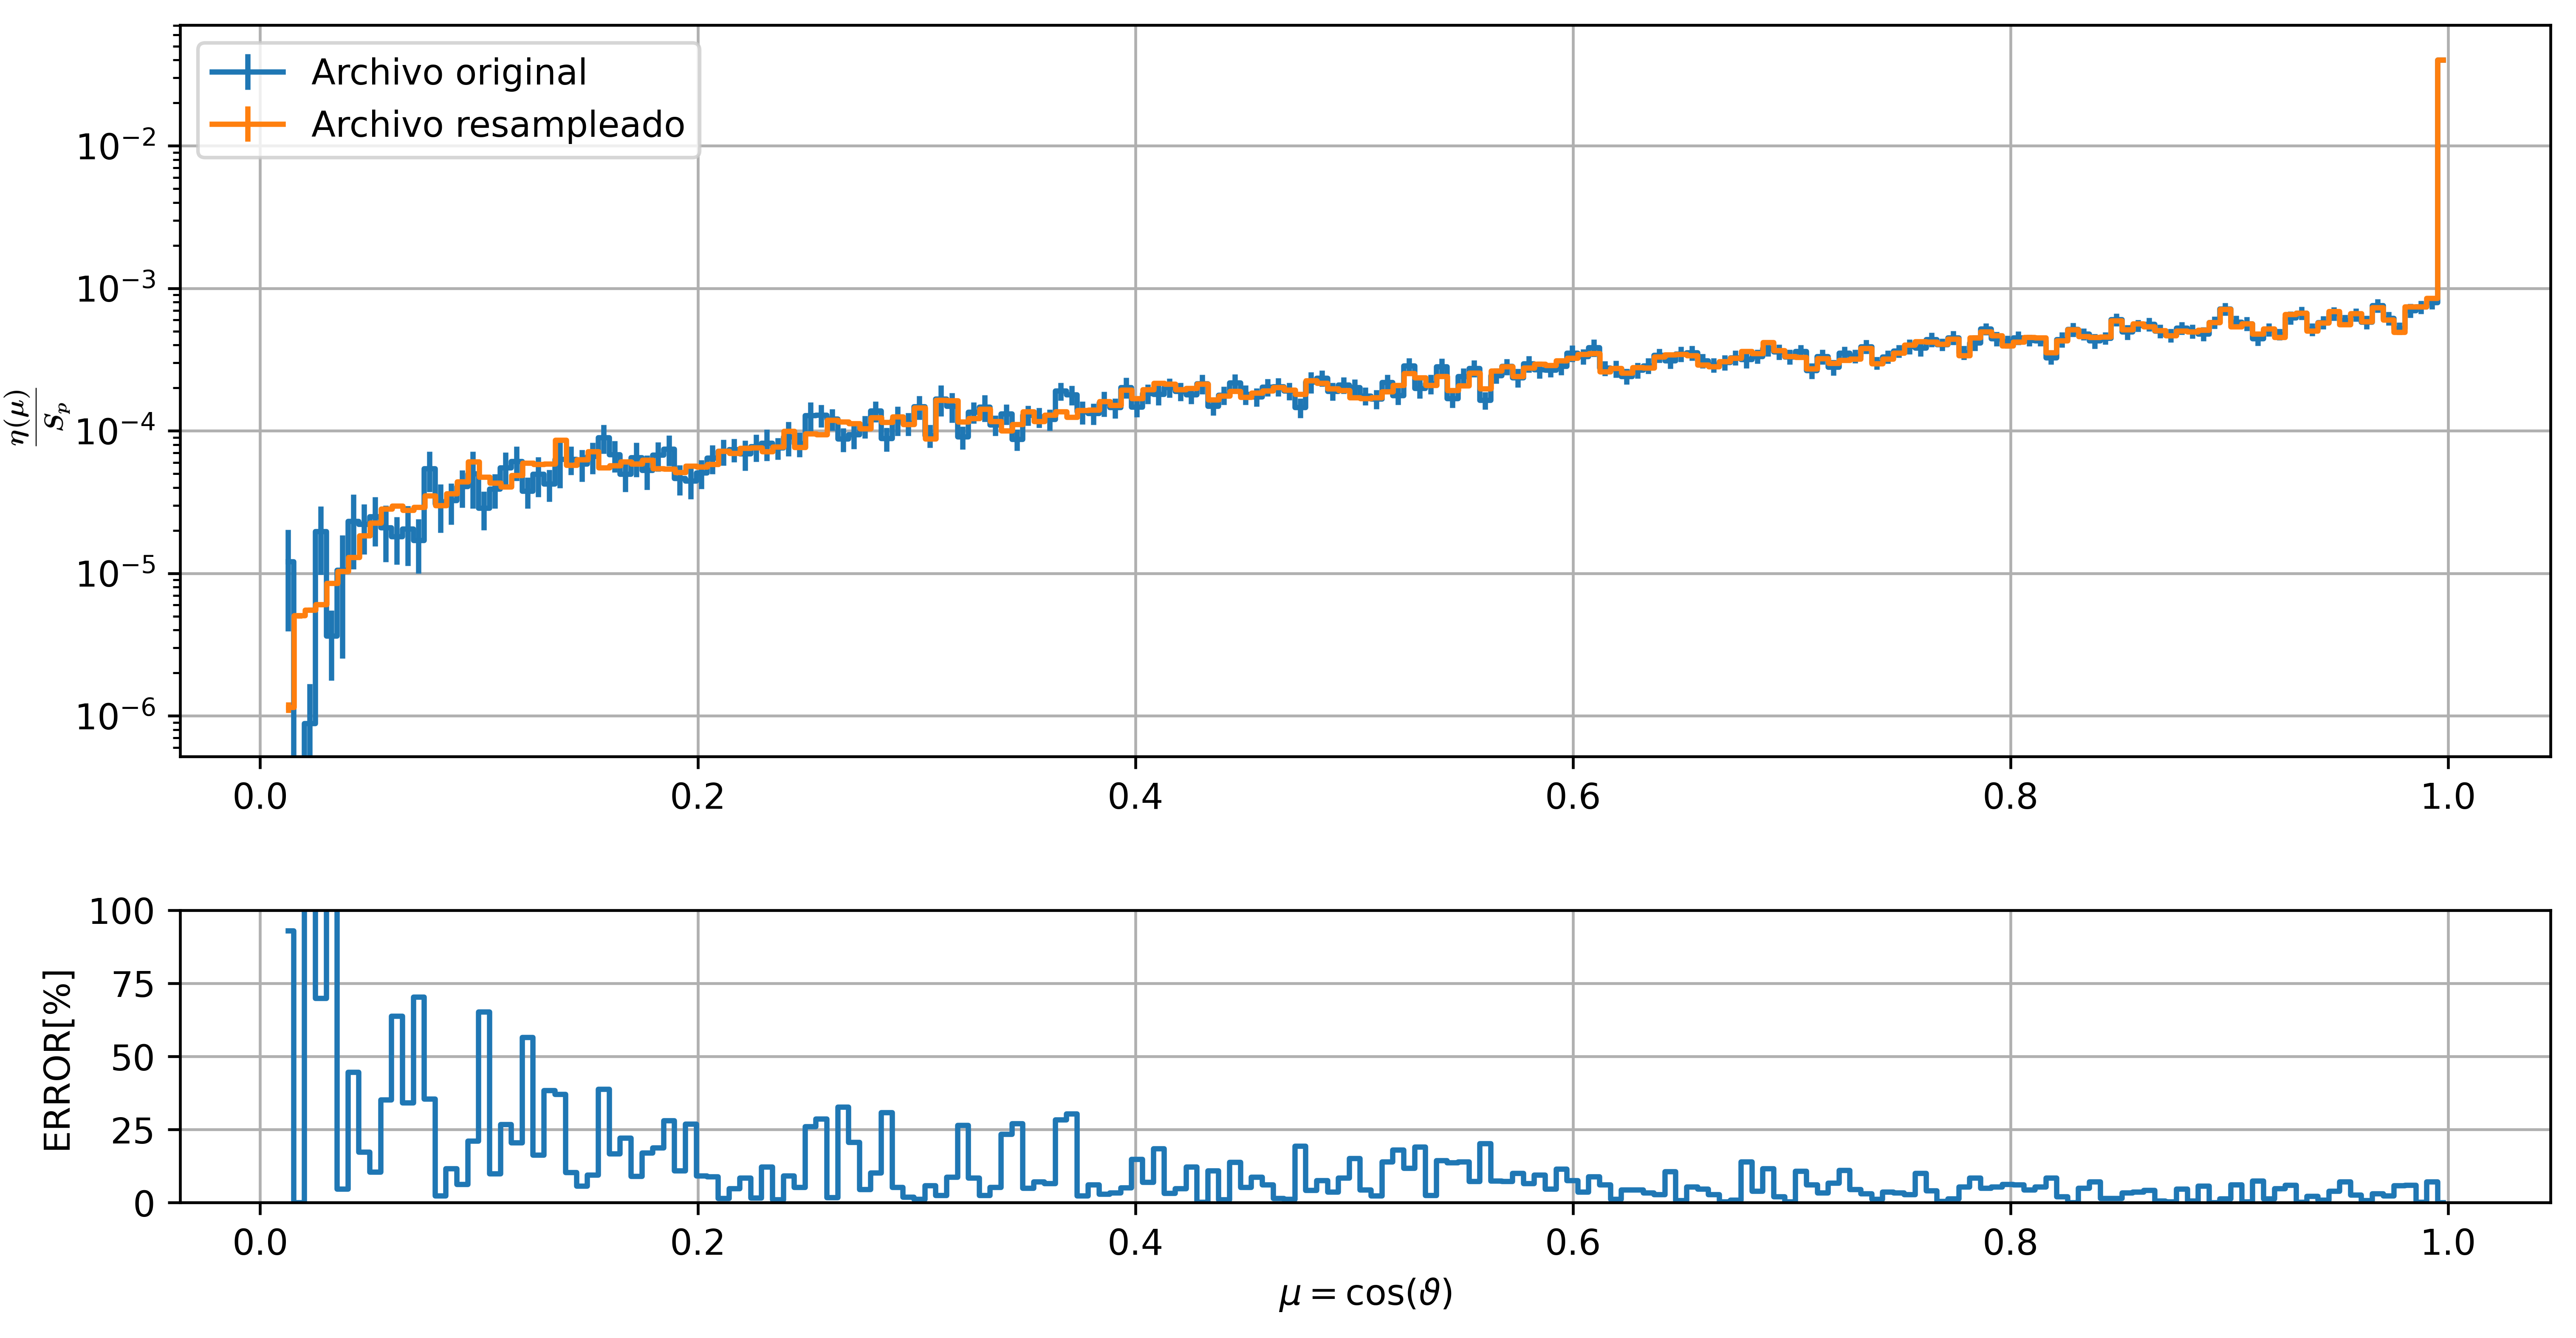
\includegraphics[width=\textwidth]{mu_4.png}
    \caption{Distribución remuestreada de $\mu$ para el caso 4 de bineado adaptativo con borde manual en $\mu \approx 1$.}
    \label{fig:mu_4}
\end{figure}

\subsection{Distribuciones espaciales $X$–$Y$}

En esta sección se detallan las distribuciones espaciales en el plano $X$–$Y$ para las 4 configuraciones analizadas. Se evalúa particularmente la capacidad de cada método para representar correctamente la geometría del sistema, especialmente en torno a la interfaz agua–vacío definida por el tubo.
    
En la Figura \ref{fig:xy_1}, correspondiente al caso 1 de bineado uniforme sin bordes, se observa un suavizado de la estadística entre regiones físicamente distintas. En particular, aparecen partículas remuestreadas en el agua que originalmente deberían haberse generado dentro del tubo de vacío. Este efecto se debe a que los histogramas uniformes no capturan la interfaz geométrica del sistema: un mismo bin puede contener partículas tanto dentro como fuera del tubo, y al remuestrear, se reparten en ambas regiones.

\begin{figure}[H]
    \centering
    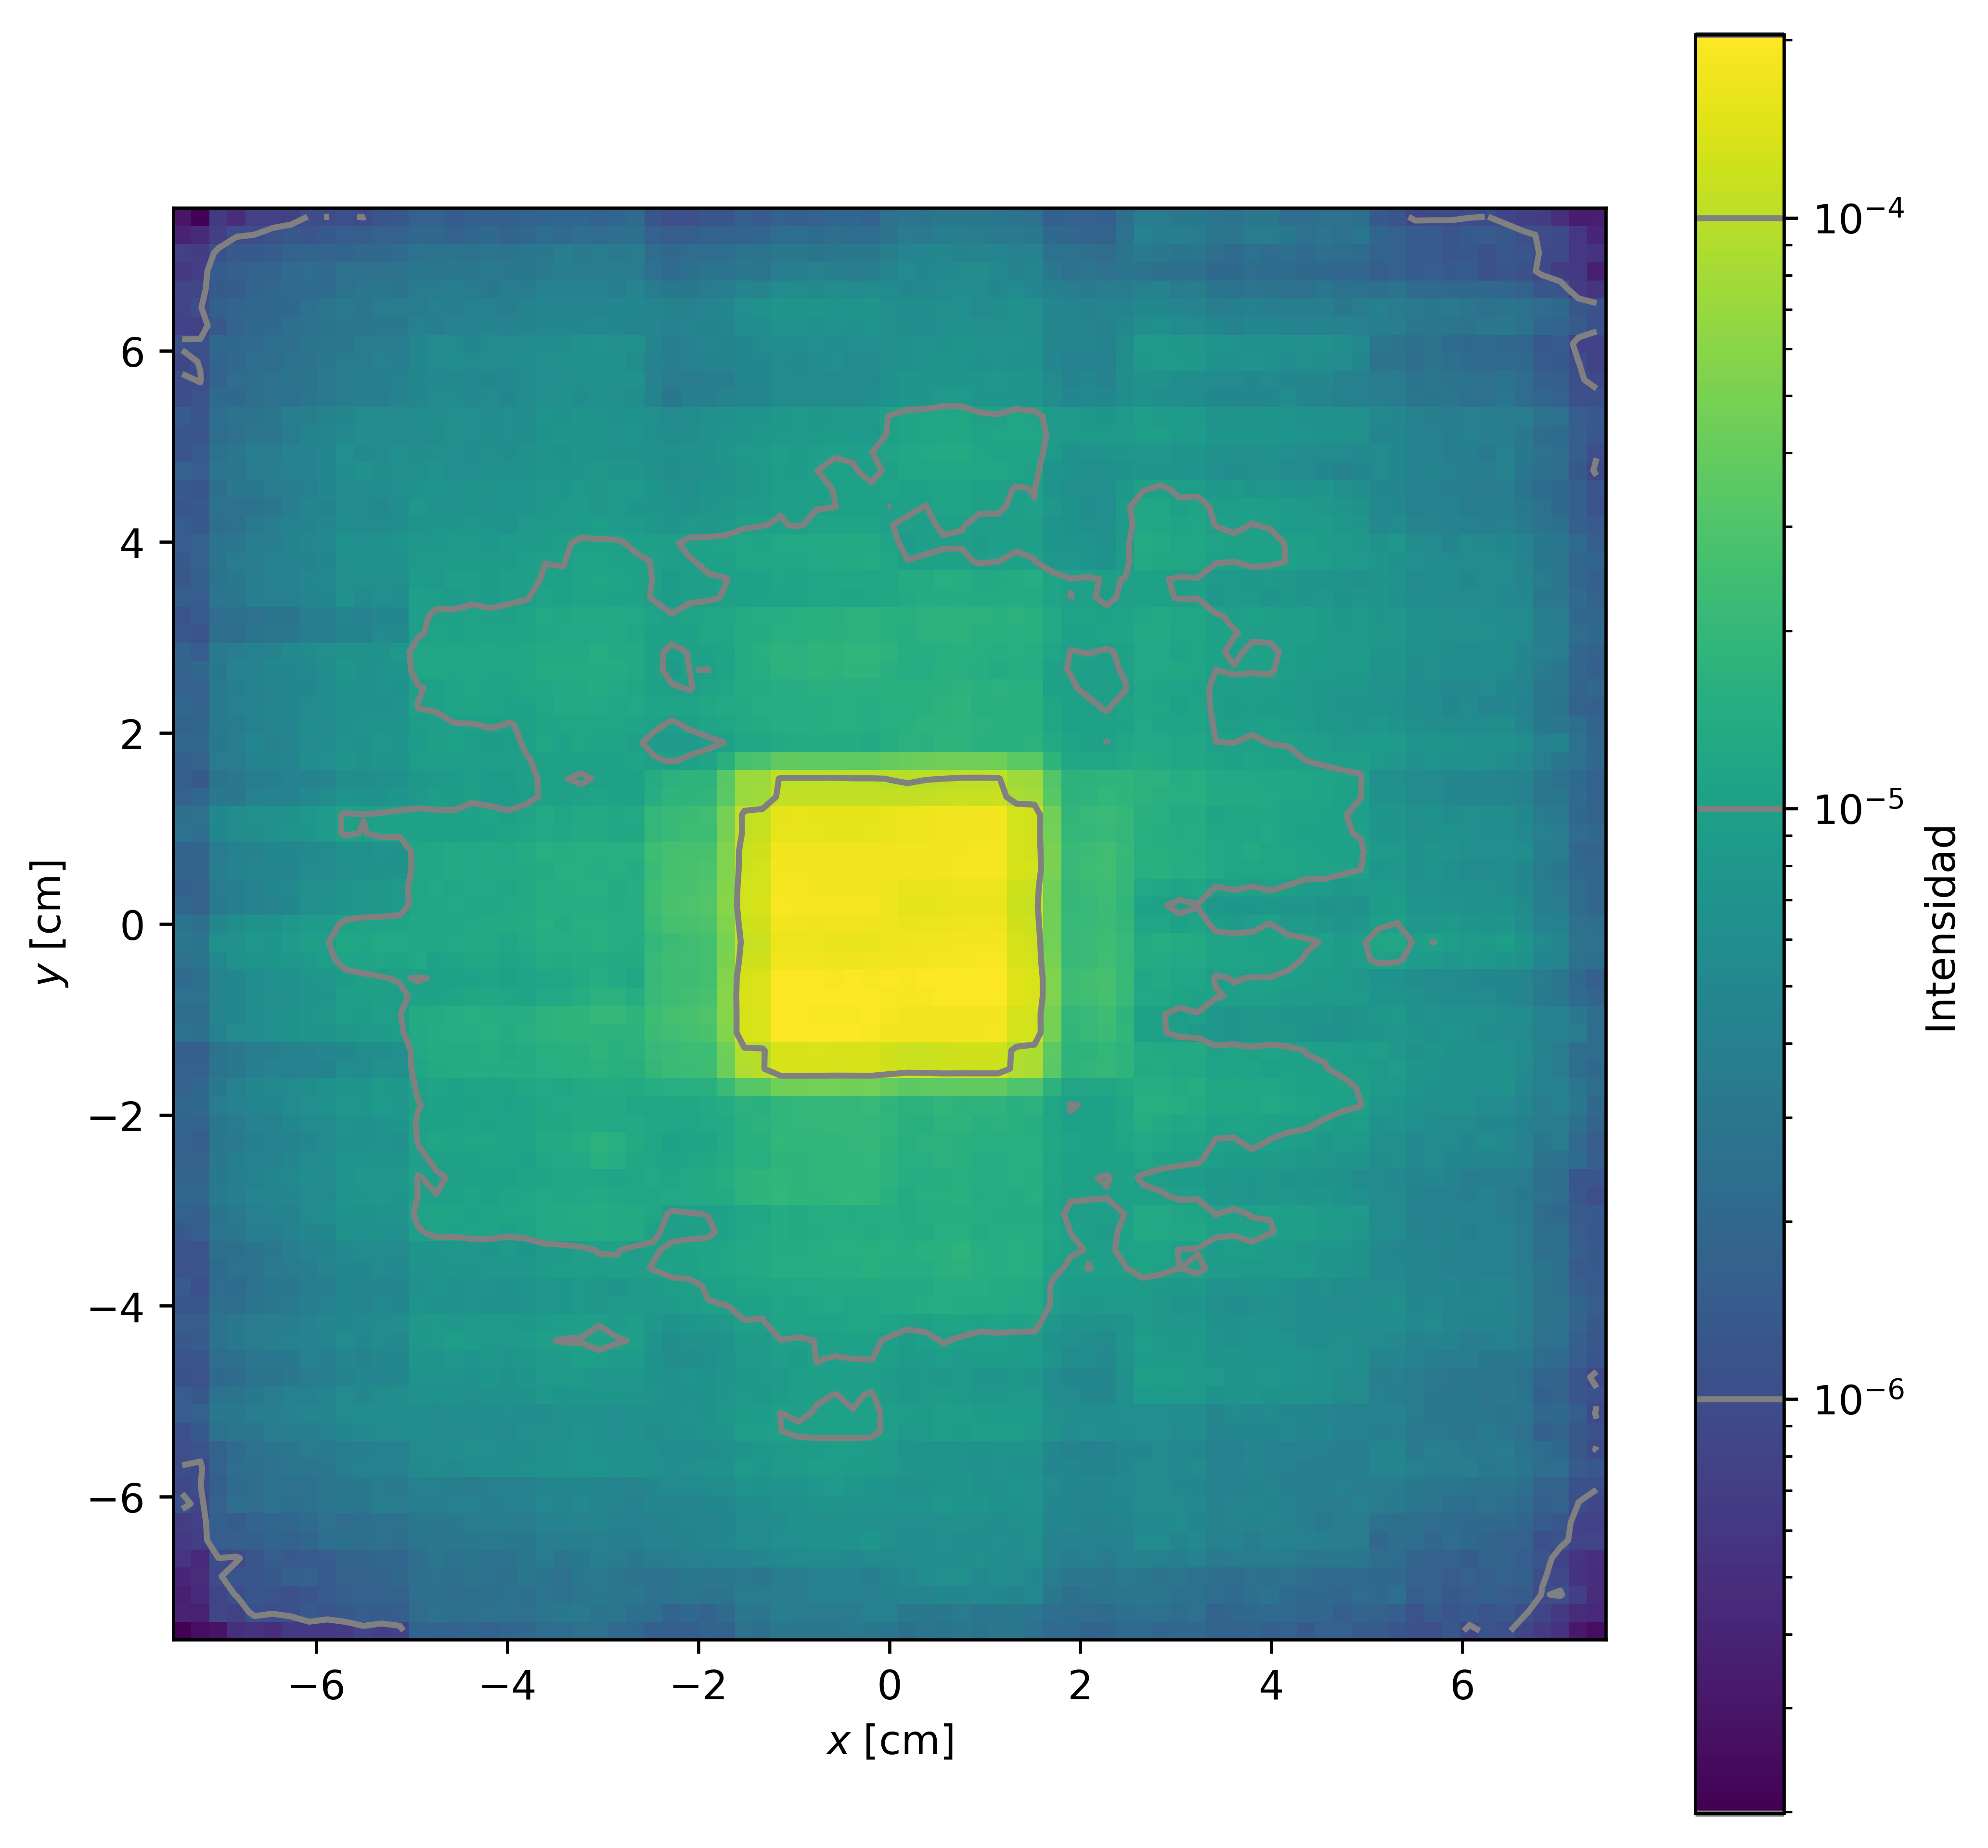
\includegraphics[width=0.6\textwidth]{xy_1.png}
    \caption{Distribución remuestreada en el plano $X$–$Y$ para el caso 1 de bineado uniforme sin bordes manuales.}
    \label{fig:xy_1}
\end{figure}

En la Figura \ref{fig:xy_2}, se incorporan bordes manuales para delimitar la región correspondiente al canal de vacío. Este ajuste mejora la segmentación espacial, concentrando la estadística dentro del tubo y evitando que partículas aparezcan en el agua. Sin embargo, se observa una estructura cuadriculada en el agua, debido a la baja estadística original combinada con la discretización forzada en grupos debido al bineado uniforme de los histogramas macro.

\begin{figure}[H]
    \centering
    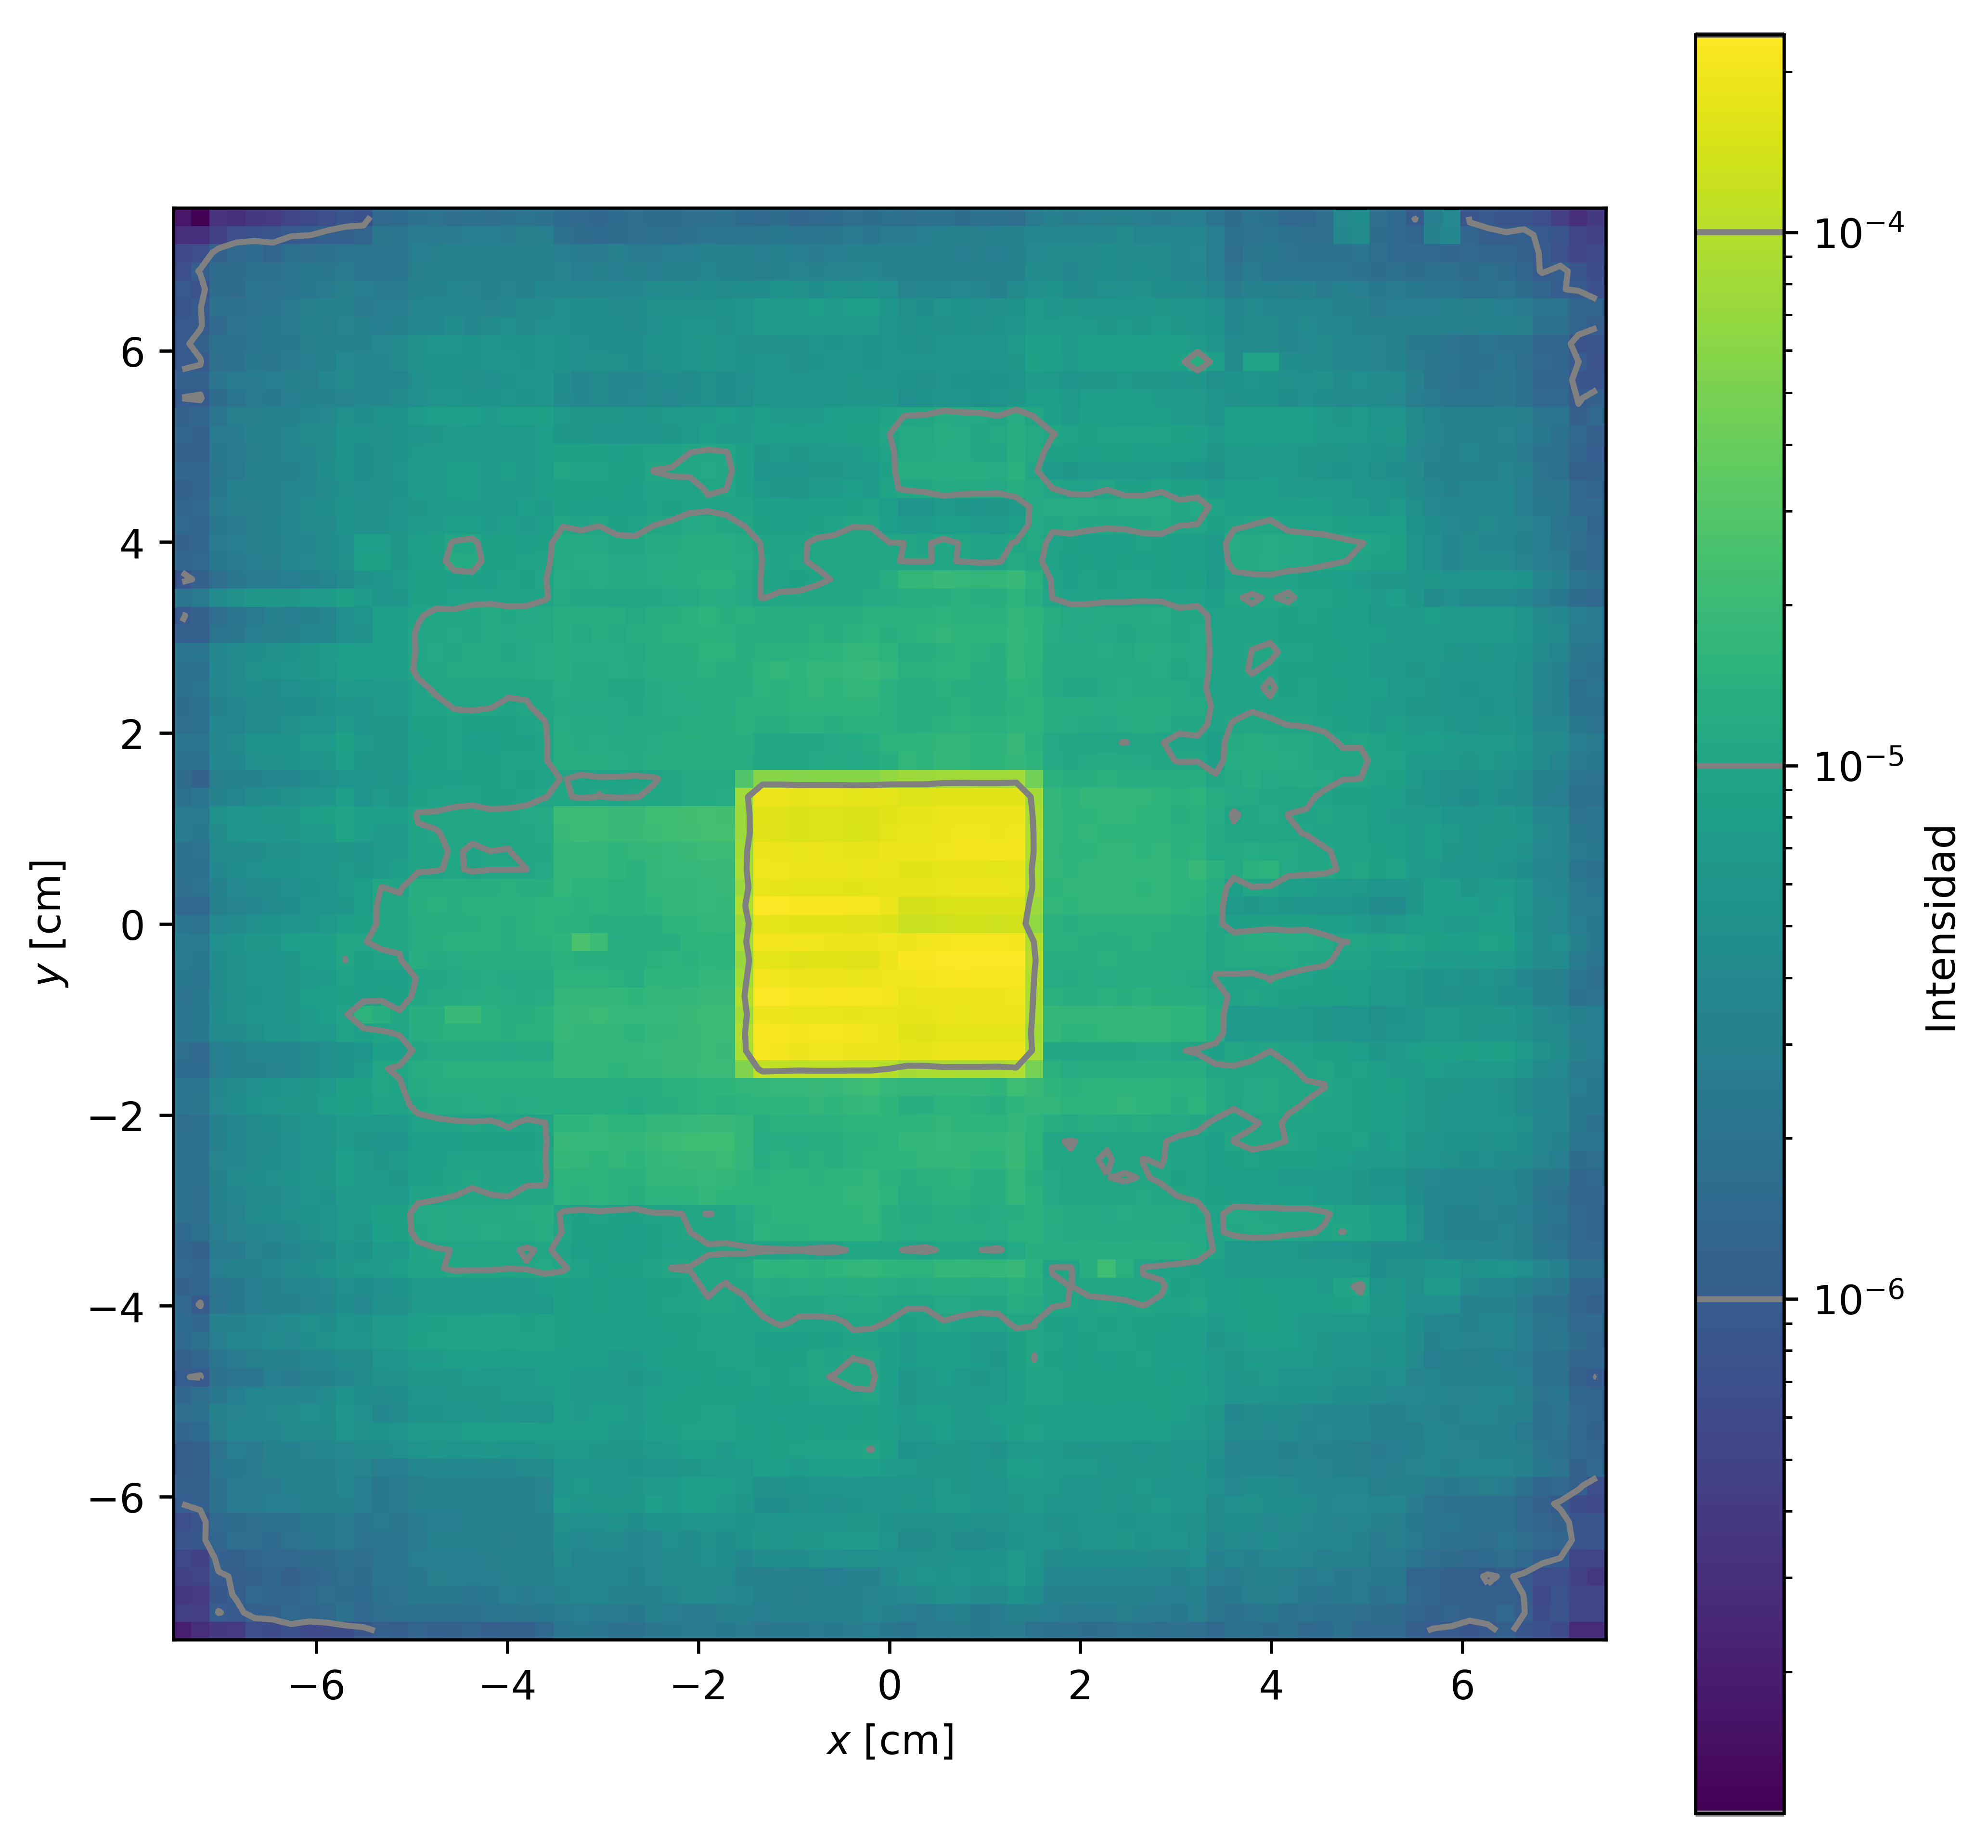
\includegraphics[width=0.6\textwidth]{xy_2.png}
    \caption{Distribución remuestreada en el plano $X$–$Y$ para el caso 2 de bineado uniforme con bordes manuales en la interfaz agua–vacío.}
    \label{fig:xy_2}
\end{figure}

La Figura \ref{fig:xy_3} presenta el resultado del caso 3 de bineado adaptativo sin bordes definidos por el usuario. En este caso, se observa que el método logra capturar adecuadamente la transición entre regiones, evitando la aparición de partículas en zonas del agua donde no correspondía. La distribución dentro del agua se muestra más homogénea que en el caso anterior, debido a que el algoritmo adaptativo no fuerza la segmentación en regiones con baja estadística.

\begin{figure}[H]
    \centering
    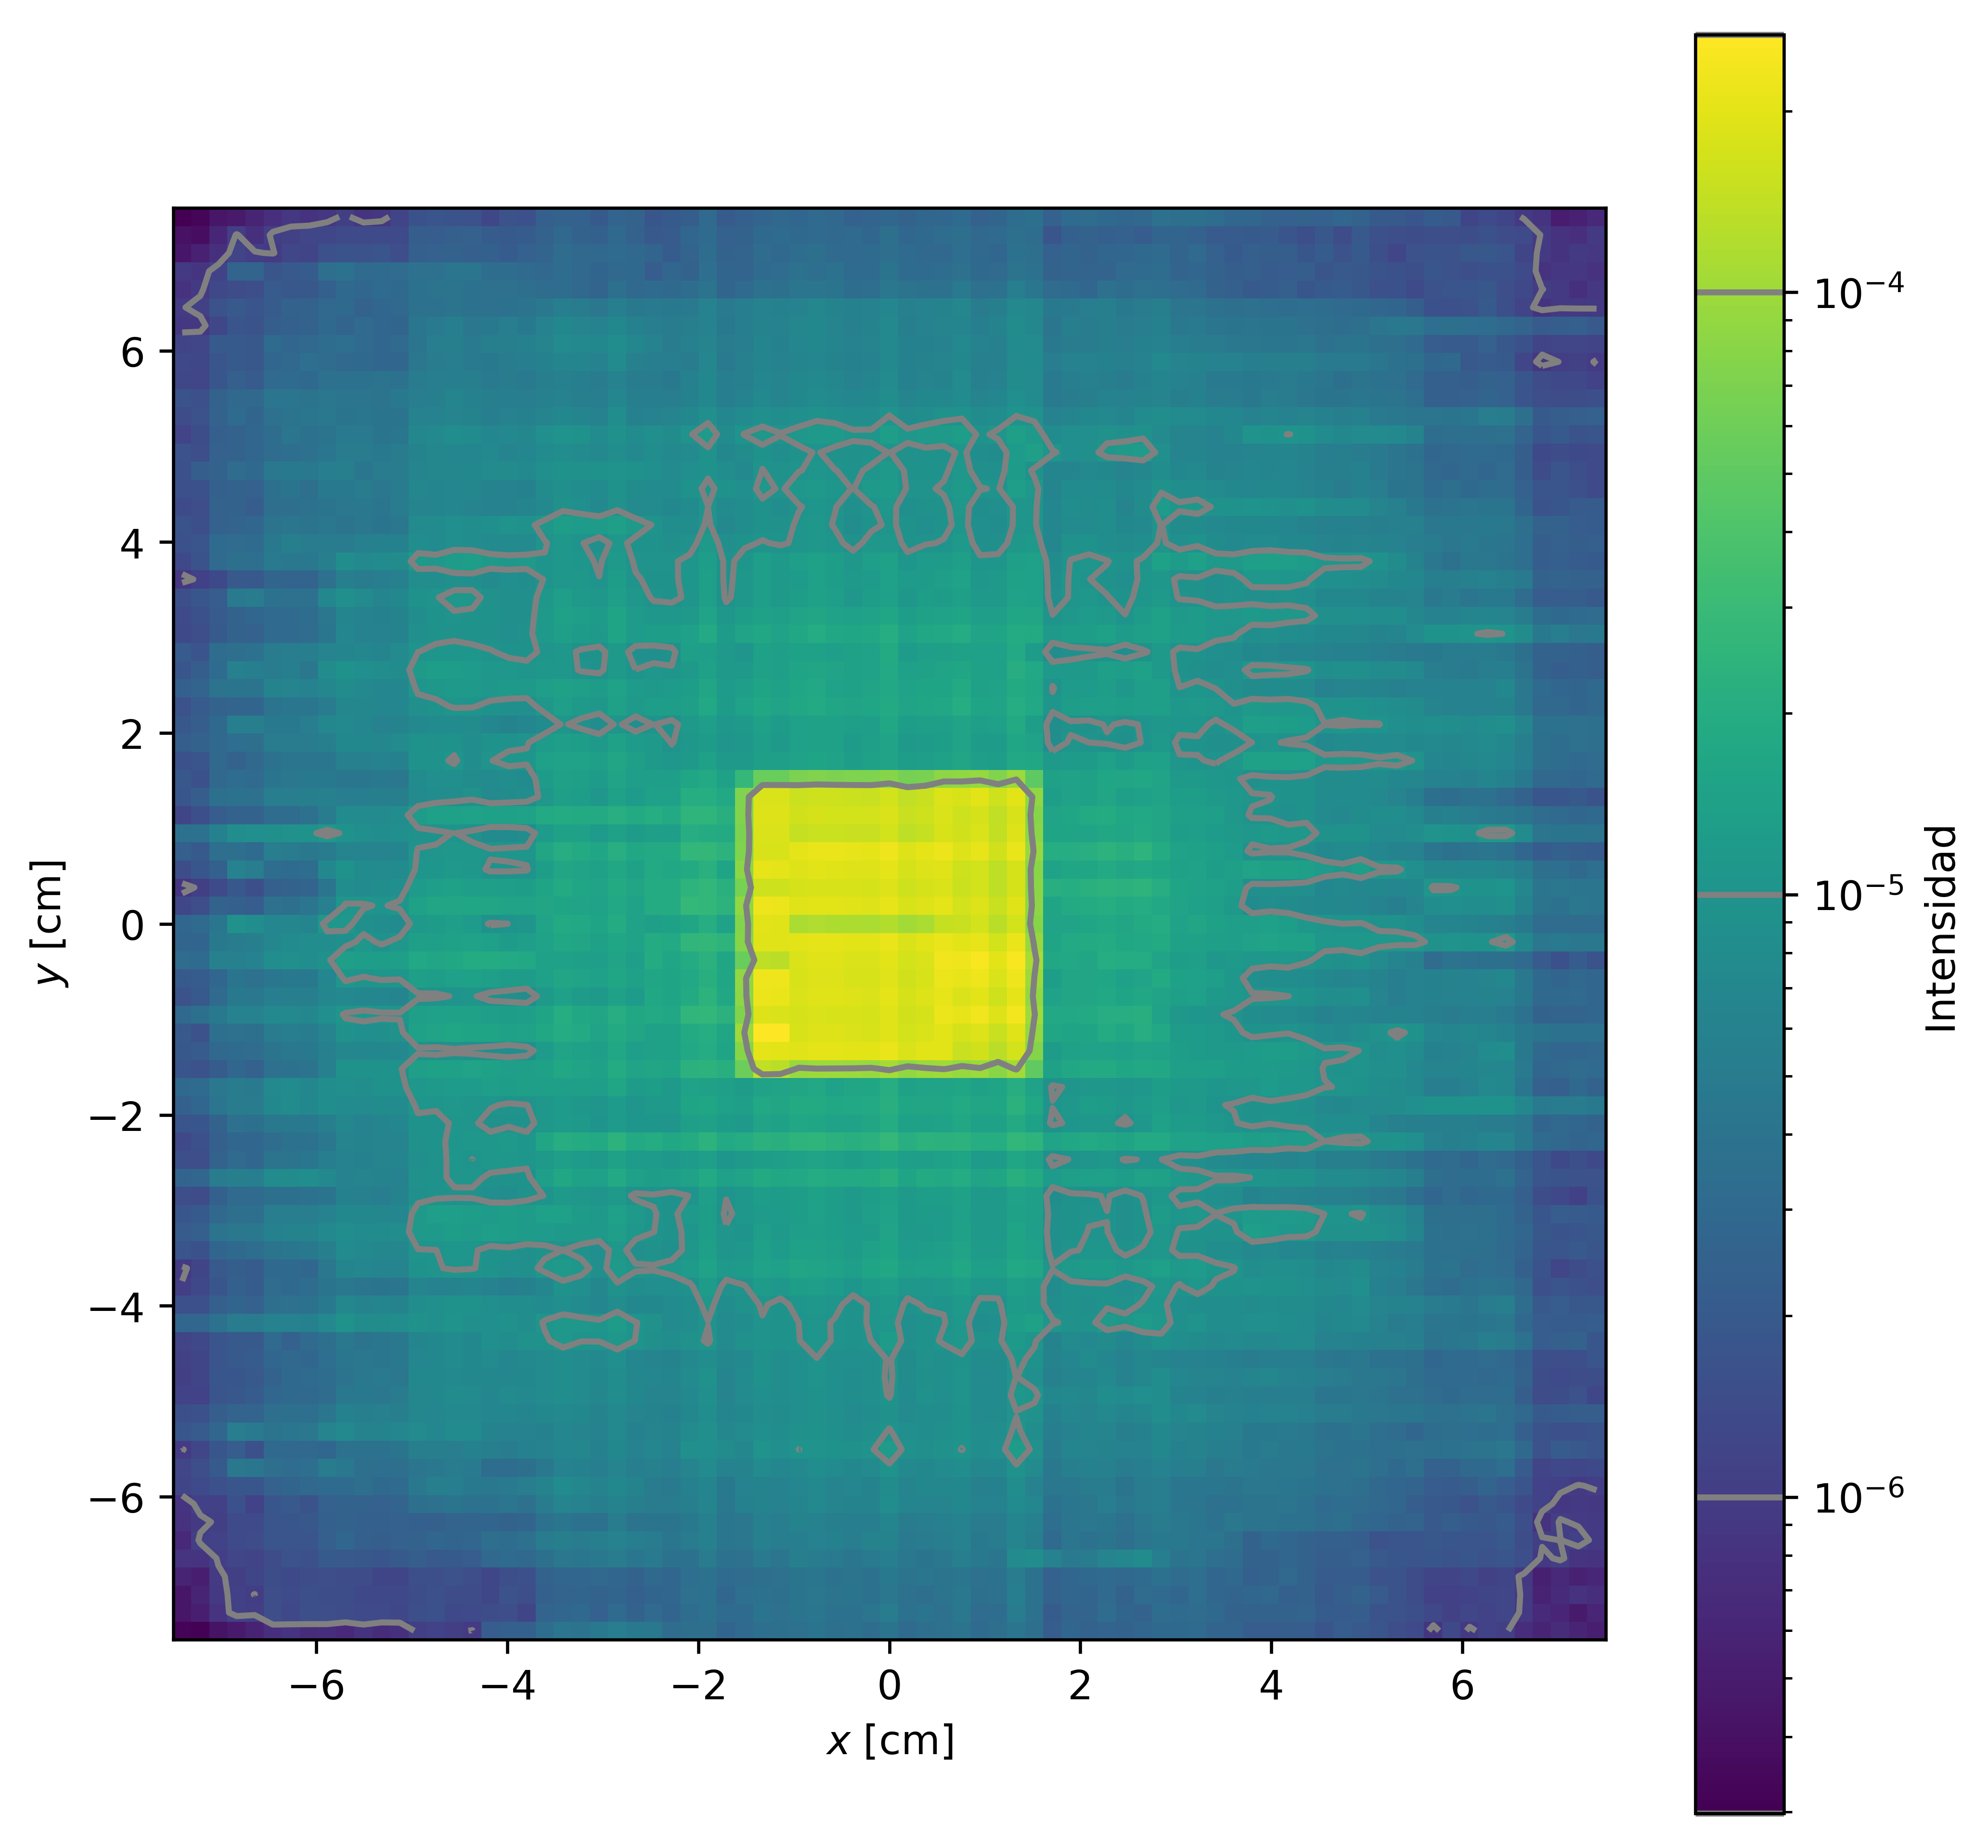
\includegraphics[width=0.6\textwidth]{xy_3.png}
    \caption{Distribución remuestreada en el plano $X$–$Y$ para el caso 3 de bineado adaptativo sin bordes manuales.}
    \label{fig:xy_3}
\end{figure}

En la Figura \ref{fig:xy_4}, se observa el caso 4 de bineado adaptativo con bordes definidos por el usuario en la interfaz. Si bien los resultados son visualmente similares a los del caso sin bordes, puede señalarse que aquí los límites del canal de vacío están representados de forma más precisa, dado que se han especificado explícitamente. No obstante, el método adaptativo sin bordes ya proporciona una aproximación razonable, por lo que la mejora en este caso es leve.

\begin{figure}[H]
    \centering
    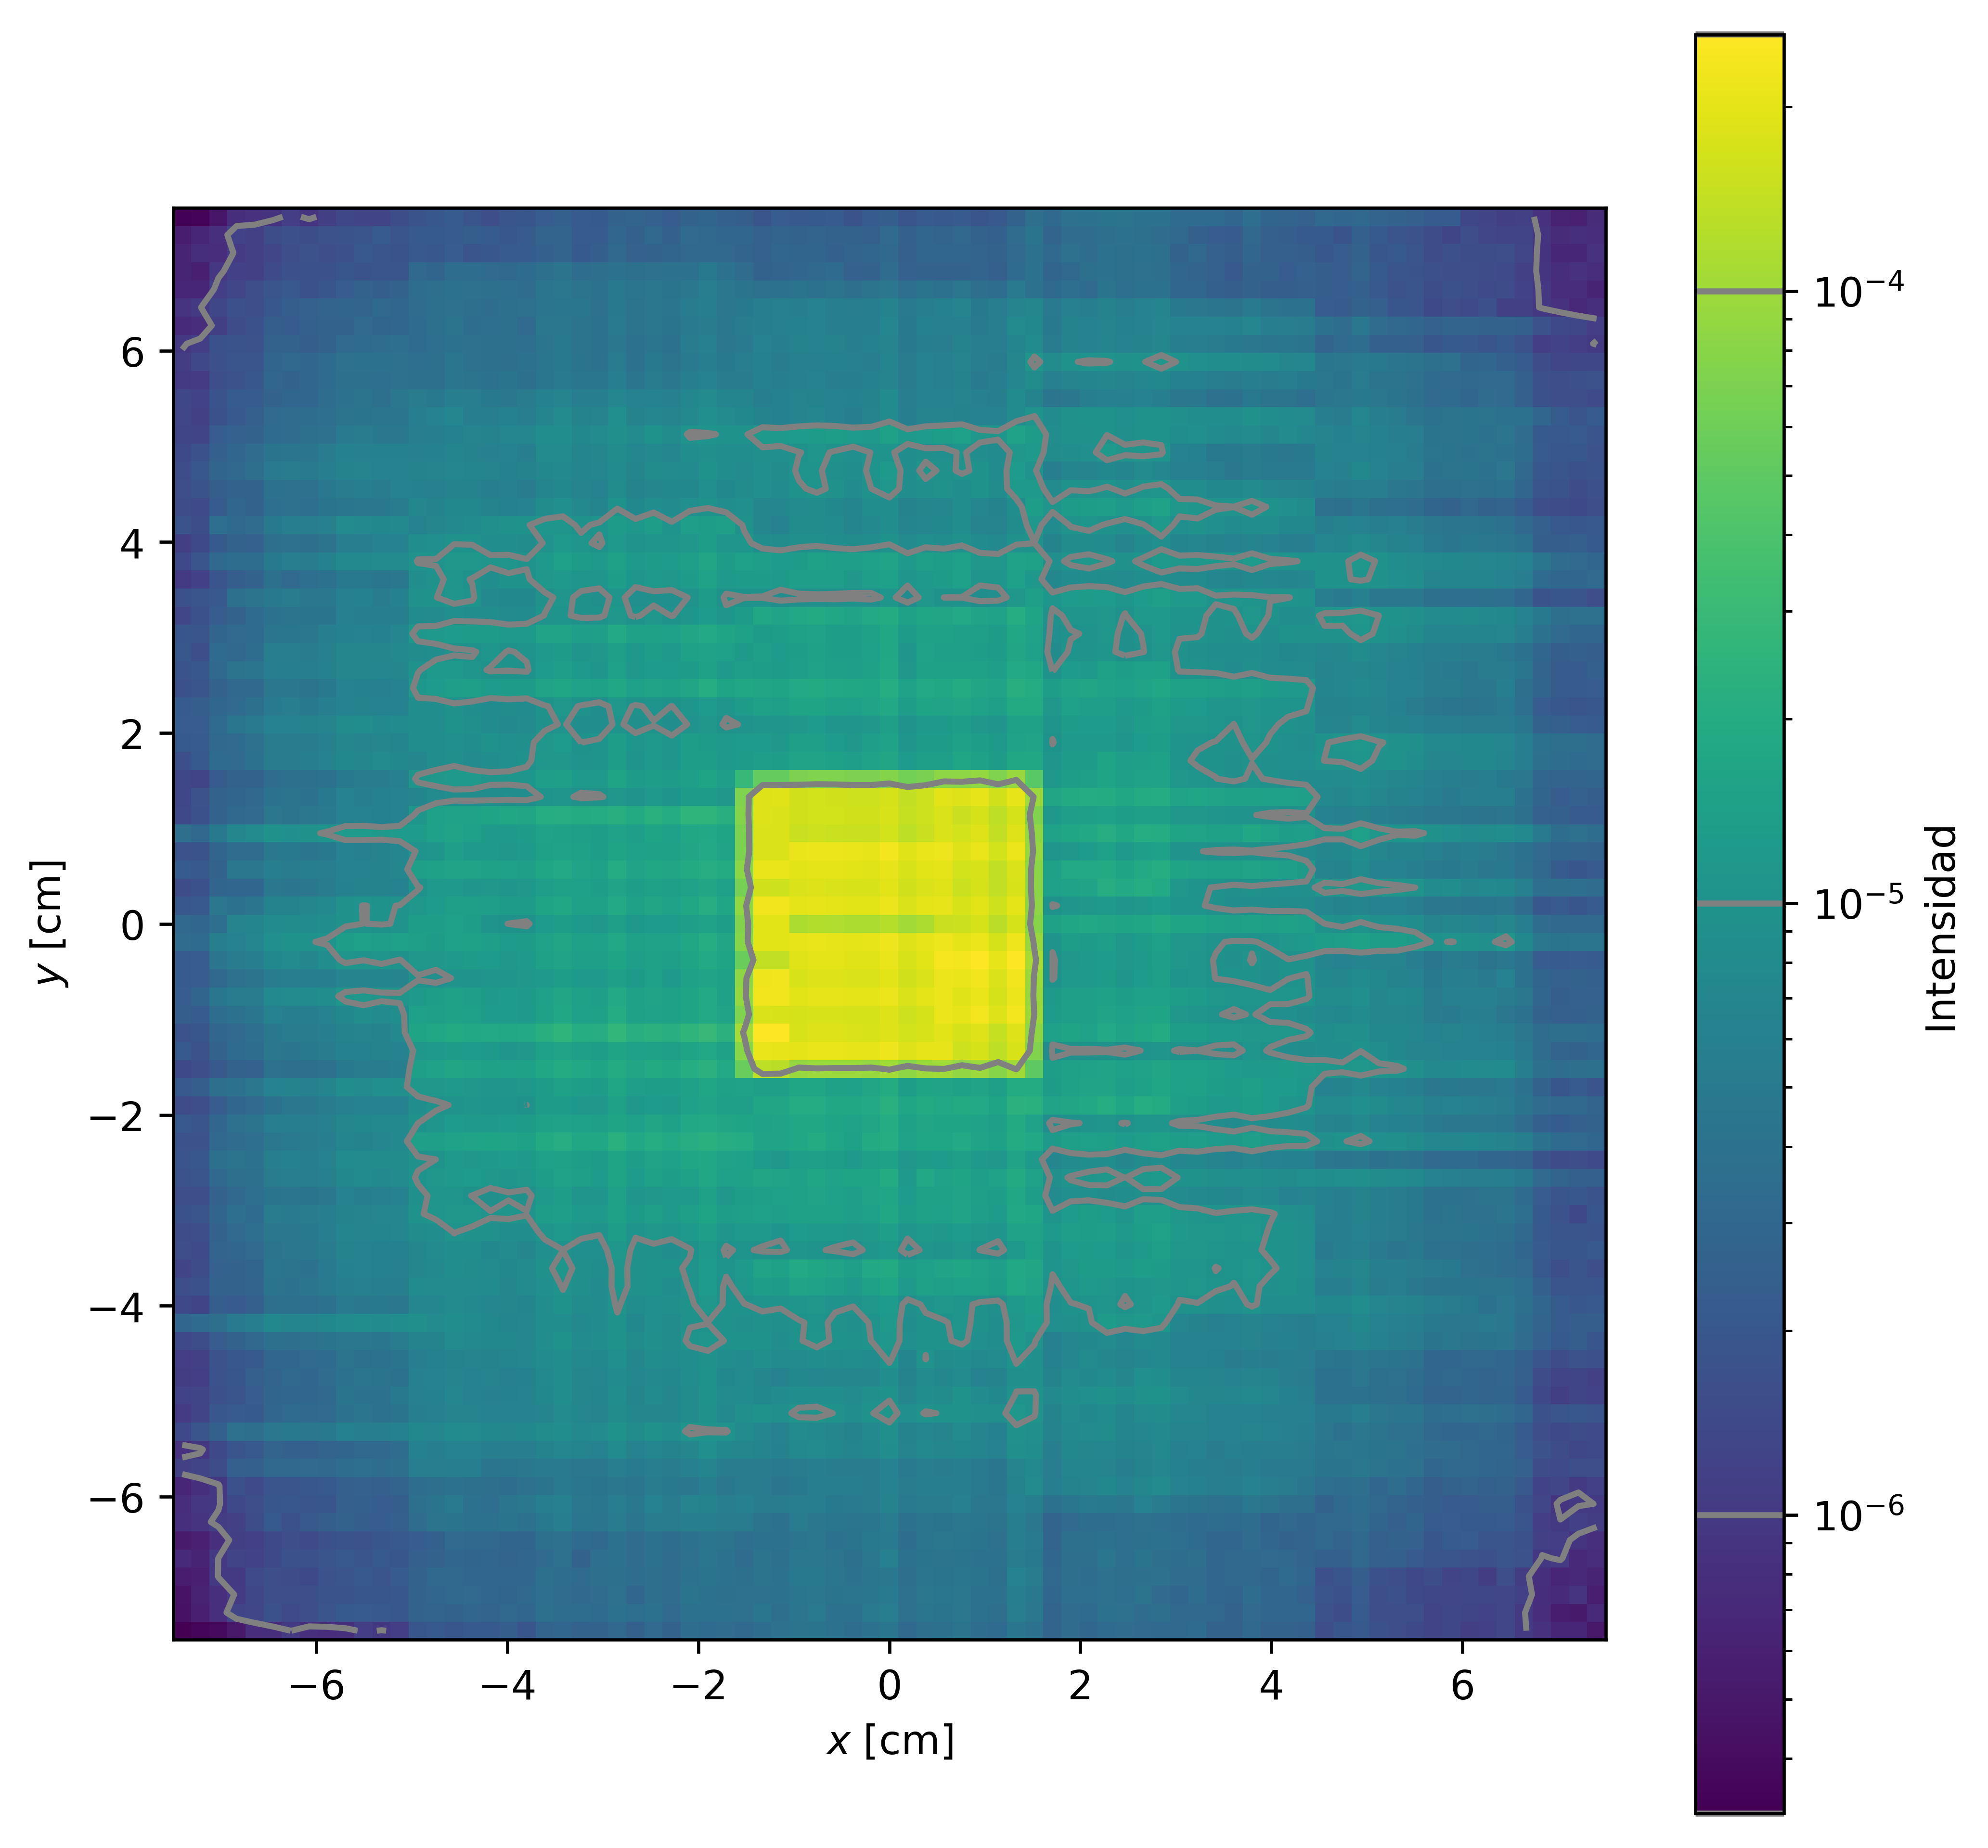
\includegraphics[width=0.6\textwidth]{xy_4.png}
    \caption{Distribución remuestreada en el plano $X$–$Y$ para el caso 4 de bineado adaptativo con bordes definidos por el usuario.}
    \label{fig:xy_4}
\end{figure}

\subsection{Análisis preliminar de los resultados}

El análisis realizado en esta sección permitió evaluar las 4 configuraciones de bineado. Se evidenció que los histogramas adaptativos ofrecen una representación más fiel del comportamiento original, incluso en ausencia de bordes manuales, en comparación con los esquemas de bineado uniforme.

Sin embargo, también se observó que la incorporación de bordes definidos por el usuario continúa siendo una herramienta útil cuando se dispone de conocimiento previo de la fuente. Estos bordes permiten guiar al algoritmo, segmentando zonas relevantes, lo que facilita a asignar mayor resolución a otras zonas del espacio de fases.

Por otro lado, se identificaron limitaciones en el esquema adaptativo. En particular, el análisis de la variable direccional $\mu$ —cuarta en el orden de las variables— evidenció un exceso de bines debido a la baja cantidad de partículas en los subconjuntos. Esta excesiva resolución produce la reproducción del ruido estadístico en lugar de su suavizado.

Para mitigar este efecto, se propone reducir progresivamente la cantidad de bines de los histogramas tanto macro como micro a medida que se avanza en el orden de segmentación. Este ajuste permitiría conservar la capacidad de detección fina en las primeras variables, mientras se evita la sobresegmentación en etapas siguientes donde la estadística es más limitada.

En la siguiente sección, se aplicará esta estrategia a modo de configuración definitiva: se volverá a procesar el archivo de partículas original empleando un esquema de segmentación jerárquica con reducción progresiva de la cantidad de bines.

\section{Procesamiento optimizado del archivo de partículas}

Con base en los resultados del procesamiento preliminar, se definió una configuración optimizada para generar la fuente distribucional. El objetivo fue preservar la fidelidad de la representación estadística, evitando al mismo tiempo la sobresegmentación de los subconjuntos que se observó en configuraciones anteriores.

Para minimizar la fragmentación del conjunto de datos, se optó por utilizar la menor cantidad posible de macrogrupos, manteniendo el orden de las variables usado previamente. La configuración seleccionada fue: 
\[
n_\text{macro} = [3, 5, 3, 3]
\]
Este esquema permitió trabajar con subconjuntos de mayor estadística en las etapas siguientes del procesamiento, mejorando así el procesamiento de los histogramas micro.

Asimismo, se eligió una cantidad reducida de microgrupos que garantizara una representación adecuada con un nivel de suavizado compatible con la estadística disponible. El esquema utilizado fue:
\[
n_\text{micro} = [30, 10, 9, 16, 4]
\]
Este conjunto es decreciente con el orden de segmentación, excepto en el caso de $\mu$, donde se incrementó el número de bines para mejorar la resolución en la zona cercana a $\mu \approx 0$.


La Figura \ref{fig:let_5} muestra la distribución remuestreada de letargía obtenida con esta configuración. Se observa una representación precisa de la delta correspondiente a la letargía mínima, así como una buena resolución en la región de termalización. En la zona intermedia, donde la densidad estadística es menor, el suavizado logrado resulta adecuado y coherente con la tendencia de la distribución original.

\begin{figure}[H]
    \centering
    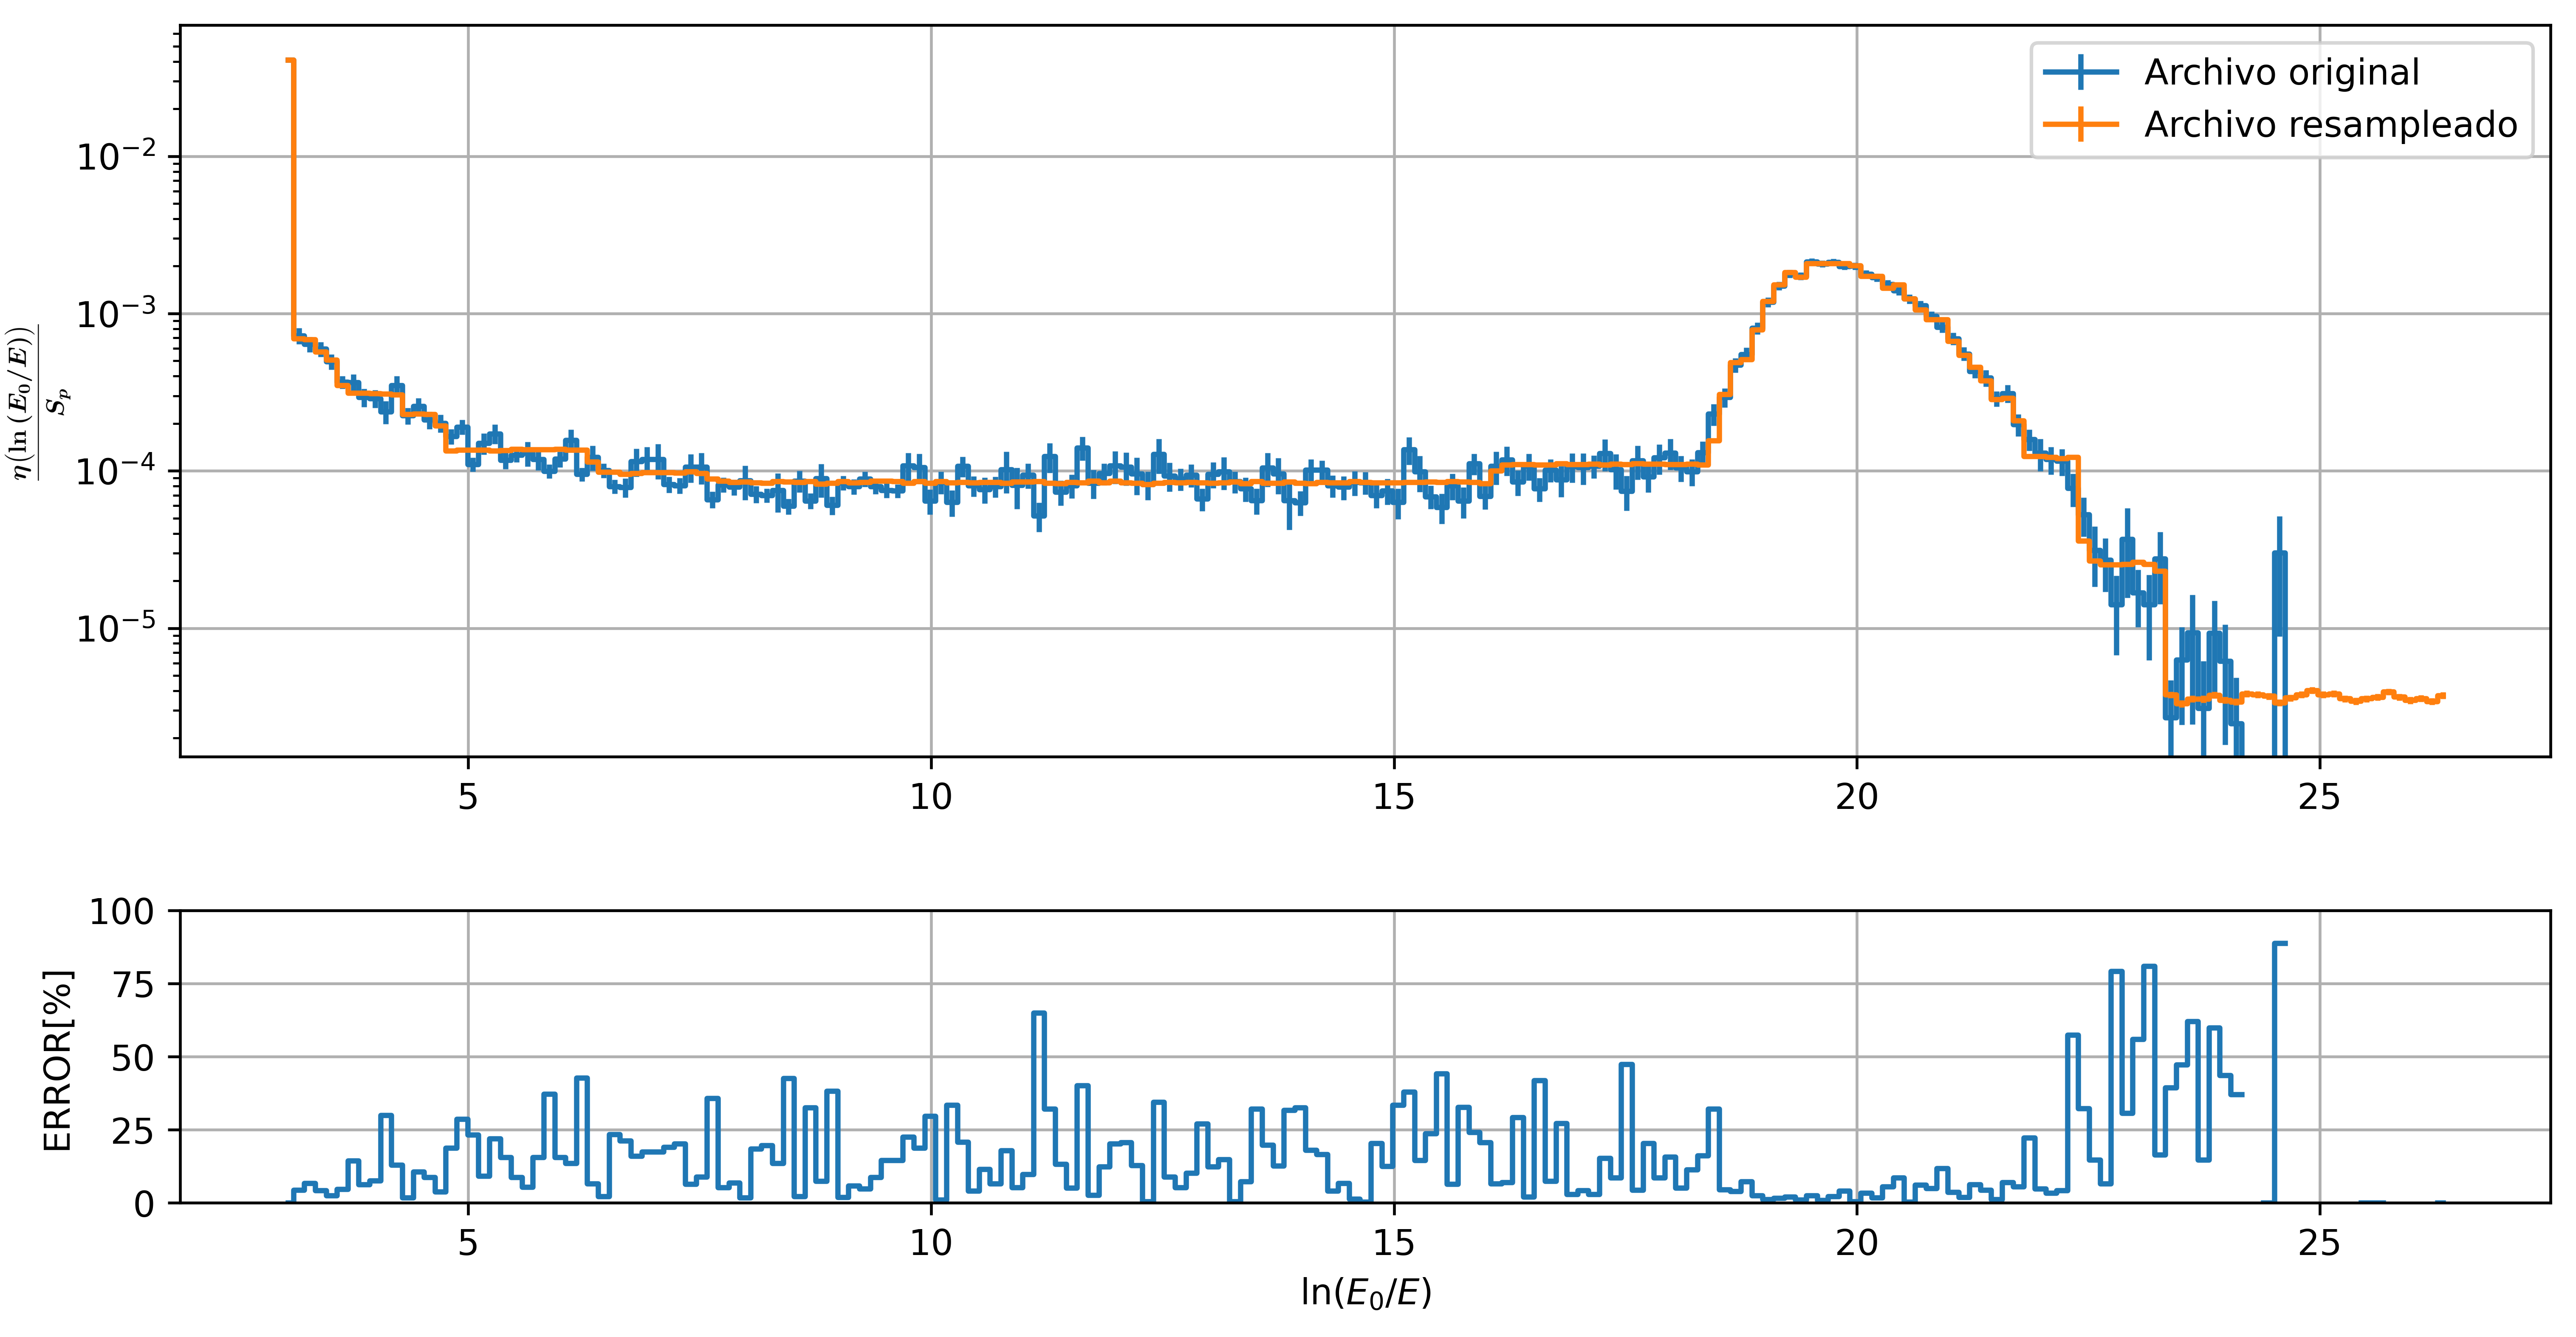
\includegraphics[width=\textwidth]{let_5.png}
    \caption{Distribución remuestreada de letargía utilizando la configuración optimizada de macro y microgrupos.}
    \label{fig:let_5}
\end{figure}

En la Figura \ref{fig:mu_5} se muestra la distribución remuestreada de $\mu$. Se obtiene una correcta representación del pico en $\mu = 1$, asociado a neutrones colimados, así como un buen seguimiento en el resto del dominio, sin evidencia de ruido estadístico excesivo.

\begin{figure}[H]
    \centering
    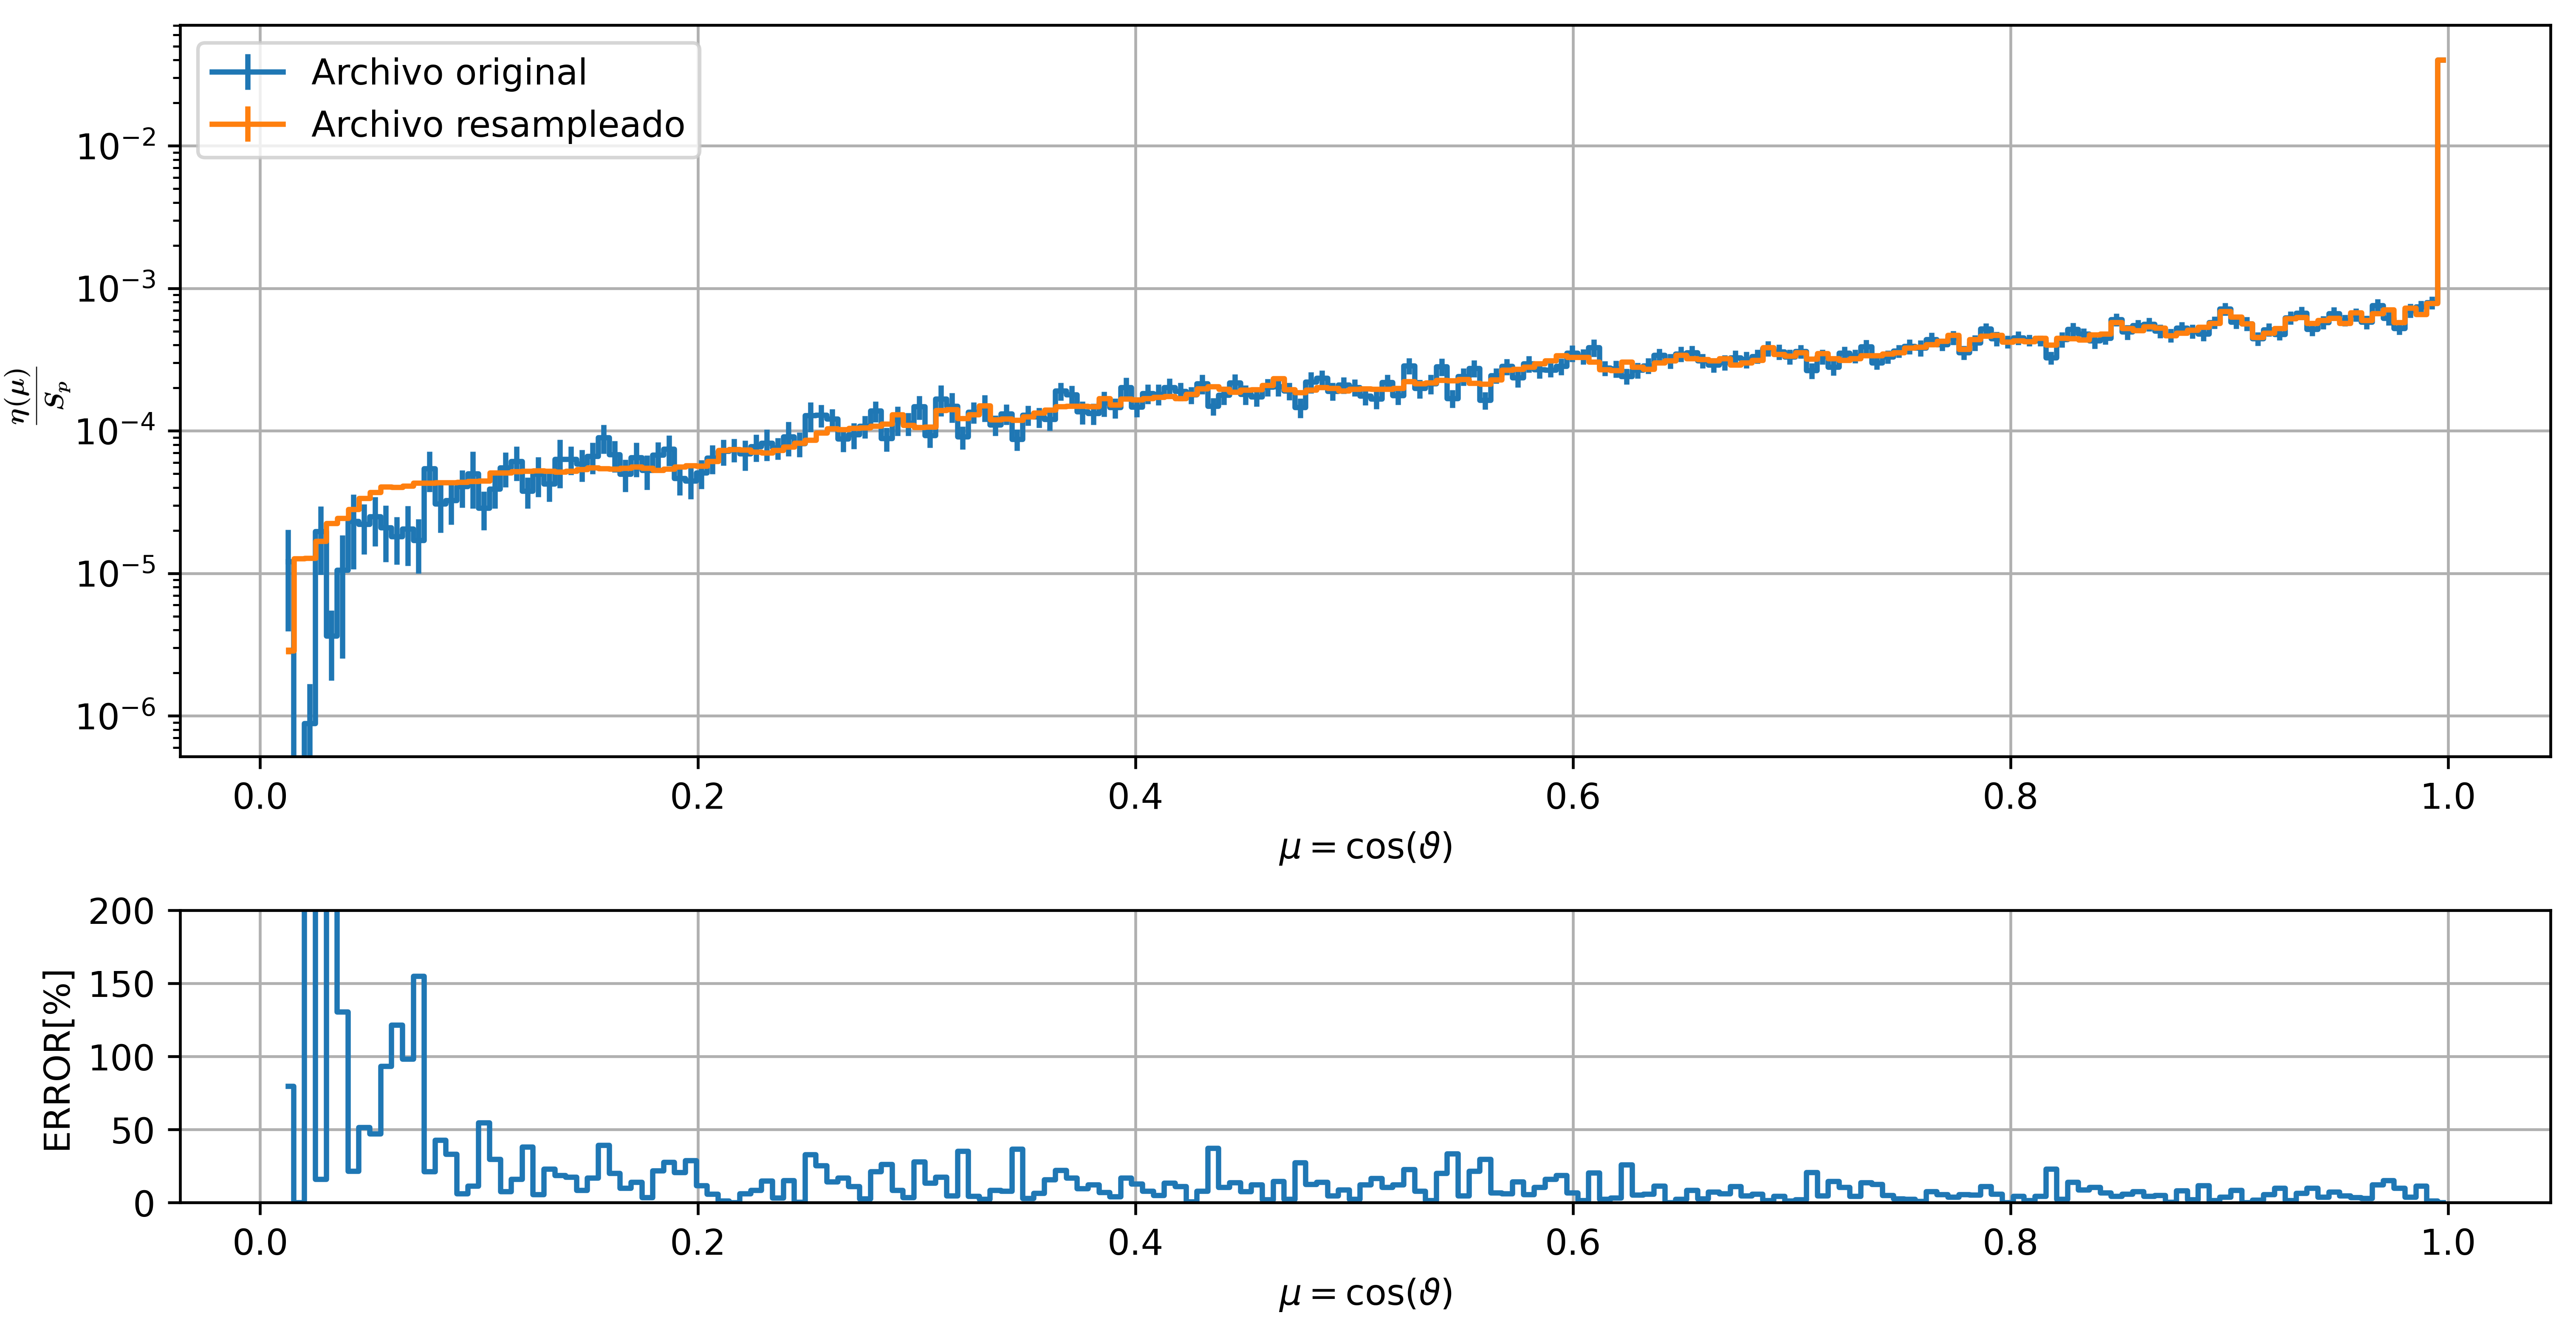
\includegraphics[width=\textwidth]{mu_5.png}
    \caption{Distribución remuestreada de $\mu$ utilizando la configuración optimizada.}
    \label{fig:mu_5}
\end{figure}

La Figura \ref{fig:xy_5} presenta la distribución espacial en el plano $X$-$Y$. Se observa una representación precisa del canal de vacío, sin generación espuria de partículas en el agua. Sin embargo, la resolución en la región del agua es inferior a la alcanzada en configuraciones con mayor cantidad de macrogrupos. Este efecto refleja el compromiso asumido: evitar segmentar en exceso regiones con baja estadística para preservar la calidad aguas abajo.

\begin{figure}[H]
    \centering
    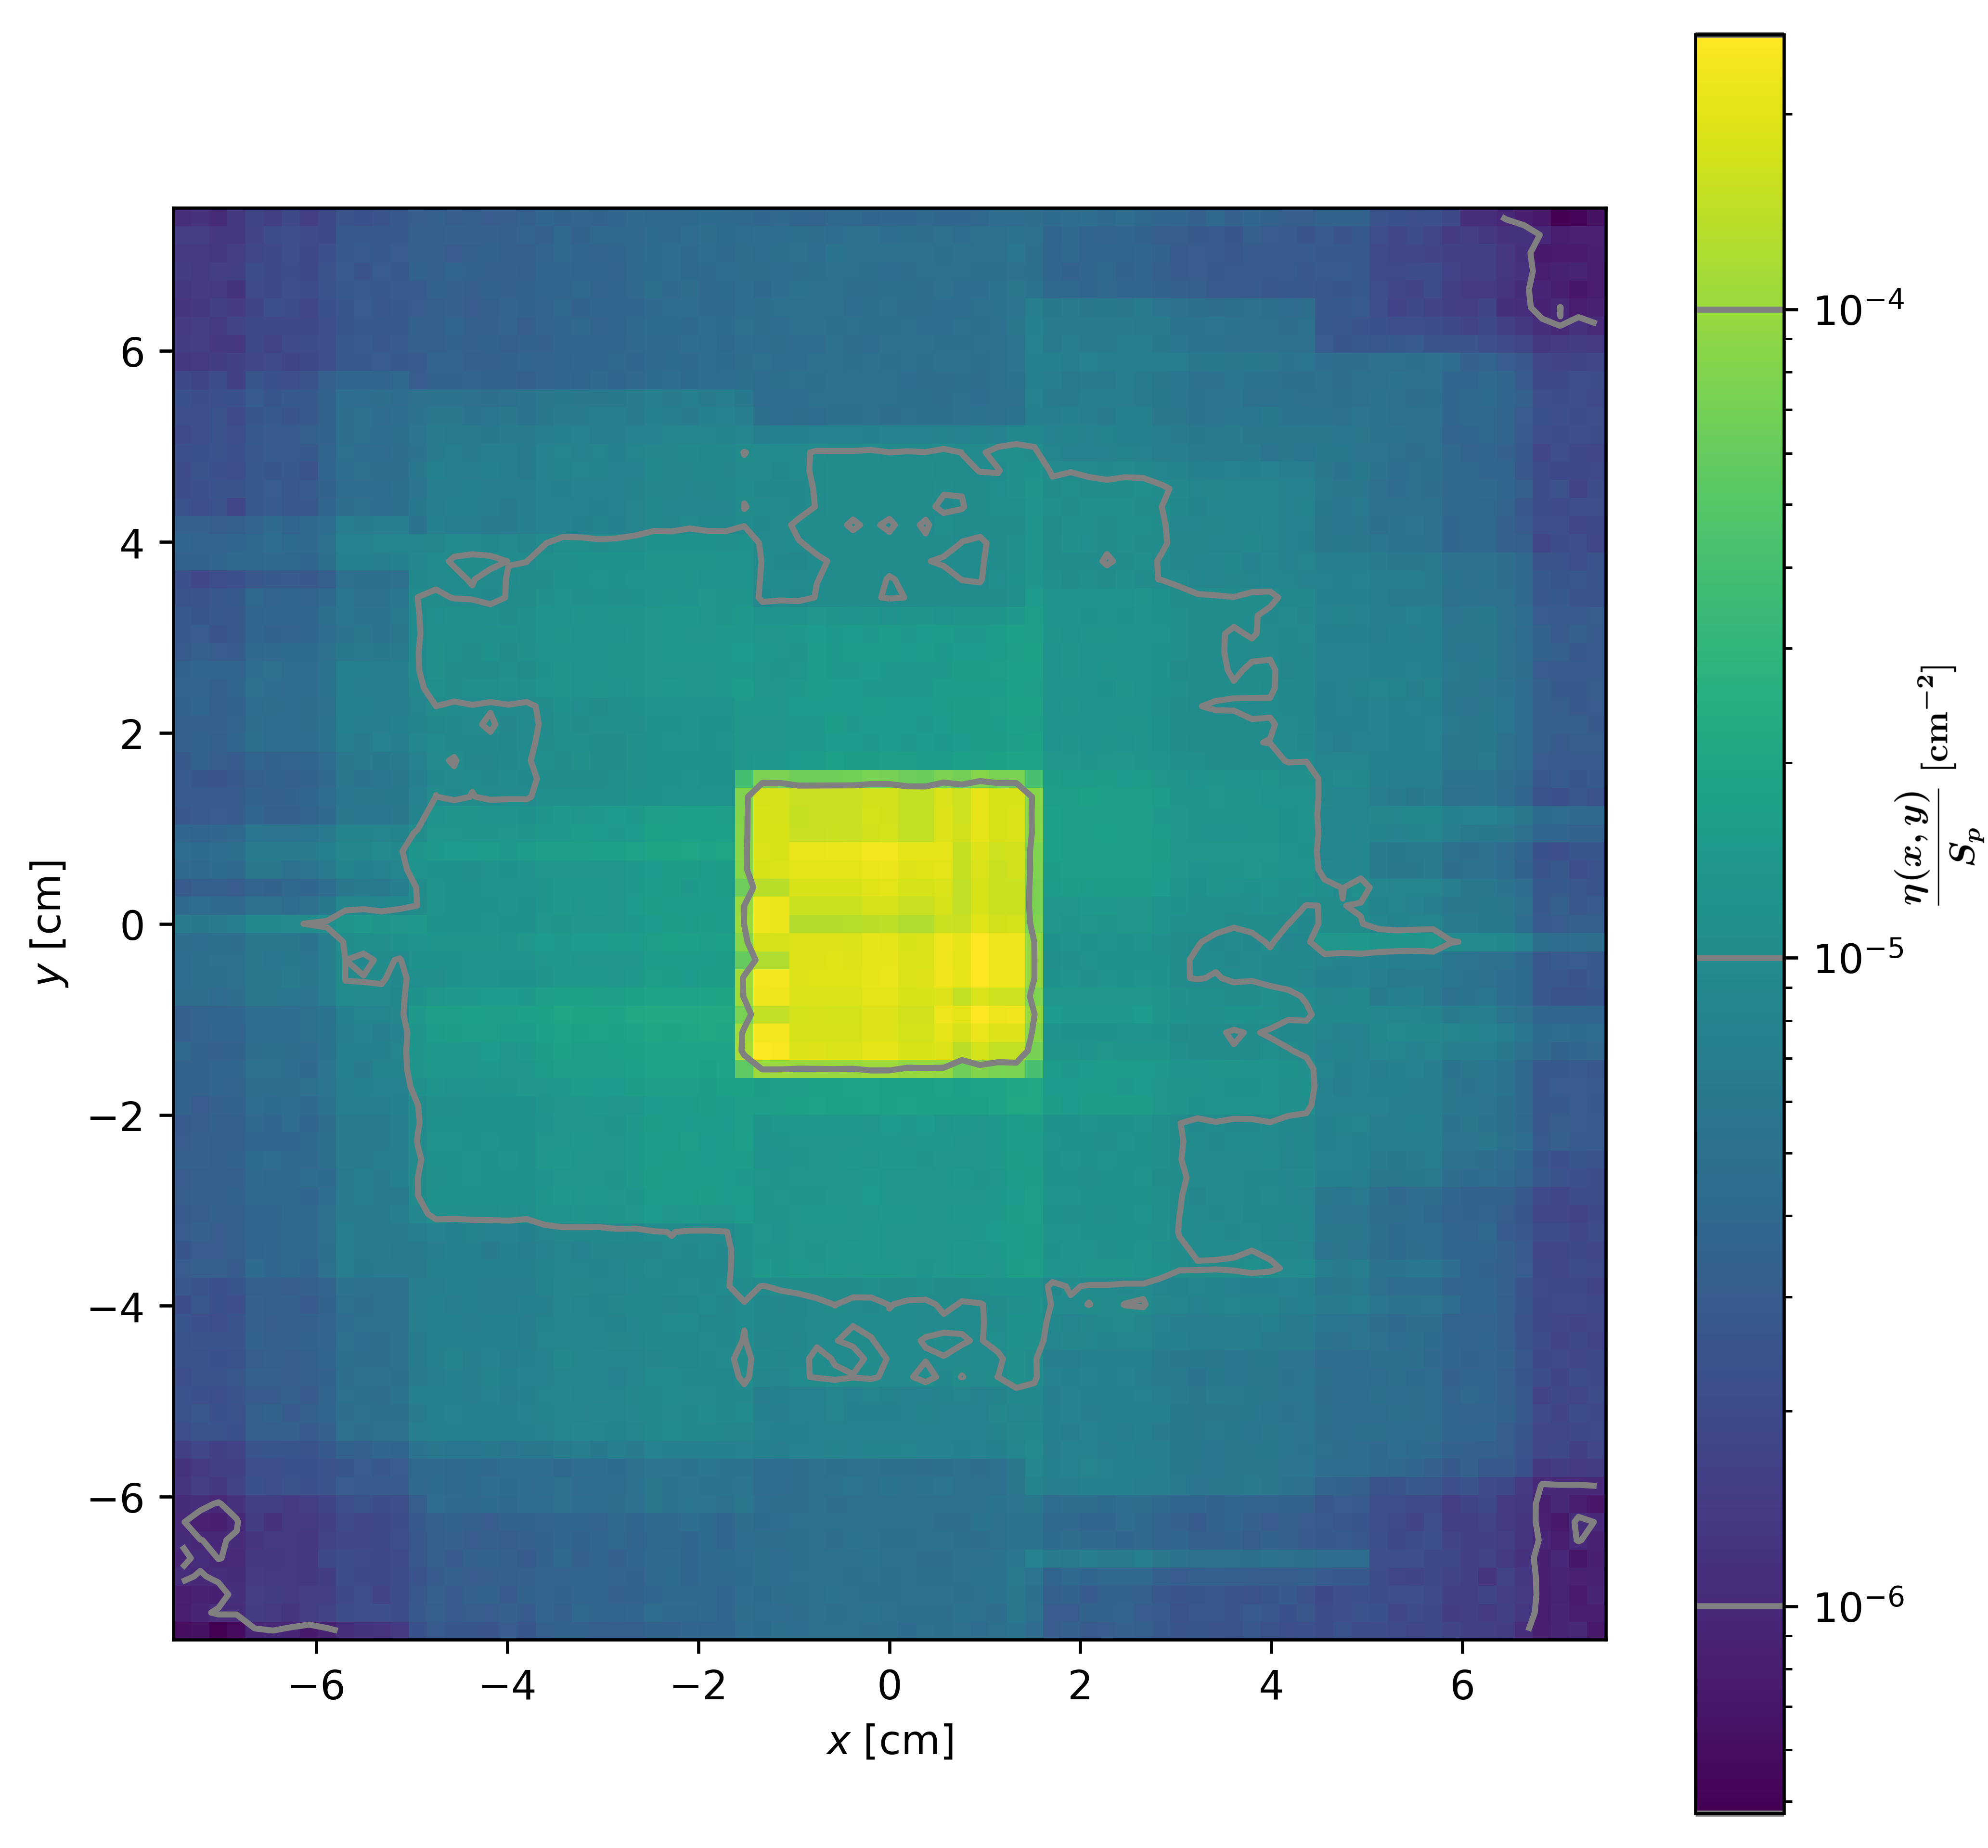
\includegraphics[width=0.6\textwidth]{xy_5.png}
    \caption{Distribución remuestreada en el plano $X$-$Y$ con configuración final optimizada.}
    \label{fig:xy_5}
\end{figure}


La configuración descrita será utilizada como base para realizar la simulación definitiva desde la superficie de acople en adelante. En la próxima sección se presentan los resultados obtenidos y se comparan contra la simulación original de referencia, ejecutada con una mayor cantidad de partículas.

\section{Resultados de la simulación comparativa}

Para validar los resultados se evaluaron distintas magnitudes físicas a lo largo del eje del sistema:

\begin{itemize}
    \item Flujo escalar a lo largo del tubo: en agua, y en vacío.
    \item Espectro energético sobre una superficie a $z = 80\,\text{cm}$.
    \item Corriente sobre una superficie a $z = 80\,\text{cm}$.
\end{itemize}

A su vez se aplicó el metodo de reducción de varianza de ventanas de peso implementado en \texttt{OpenMC} para mejorar la estadística en el agua.

\subsection{Comparación del perfil de flujo a lo largo del canal}

Con el objetivo de validar la fuente distribucional generada, se realizó una simulación de referencia desde el inicio del conducto, utilizando una cantidad elevada de partículas para asegurar una buena convergencia estadística, según se muestra en la Figura~\ref{fig:esquema_remuestreo}. A partir de esta simulación se obtuvo el perfil de flujo original a lo largo del canal.

Posteriormente, se utilizó la fuente distribucional construida en la sección anterior y se ejecutó una nueva simulación iniciando desde la superficie ubicada a $z = 15$cm. Esta corrida fue llevada adelante hasta alcanzar también una buena convergencia, permitiendo así una comparación directa entre ambos resultados.

La Figura \ref{fig:flujo_comparacion} muestra los perfiles de flujo escalar obtenidos en ambas regiones del conducto: la región de agua moderadora (\ref{fig:flujo_agua}) y el canal de vacío (\ref{fig:flujo_vacio}), junto con el error relativo porcentual.

\begin{figure}[H]
    \centering
    \begin{subfigure}[t]{0.48\textwidth}
        \centering
        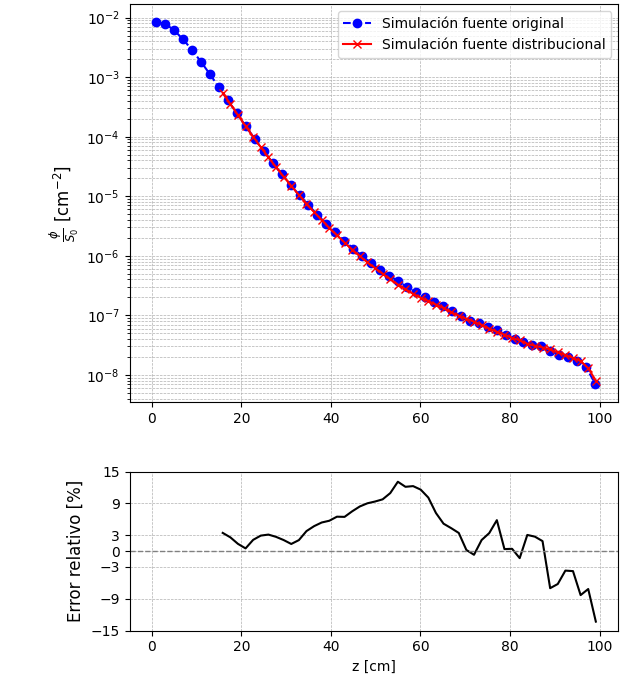
\includegraphics[width=\textwidth]{flujo_agua.png}
        \caption{Región de agua.}
        \label{fig:flujo_agua}
    \end{subfigure}
    \hfill
    \begin{subfigure}[t]{0.48\textwidth}
        \centering
        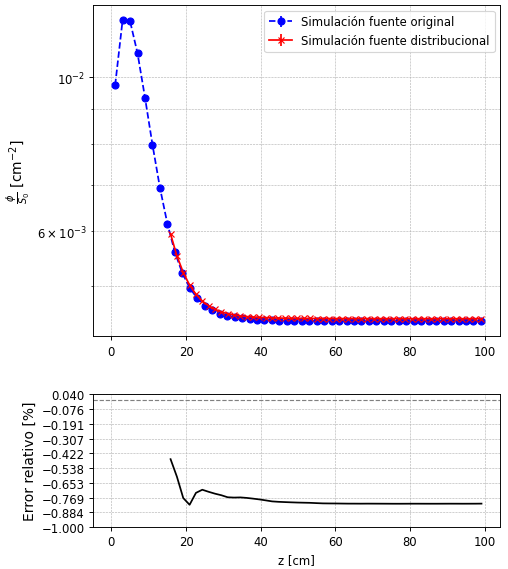
\includegraphics[width=\textwidth]{flujo_vacio.png}
        \caption{Canal de vacío.}
        \label{fig:flujo_vacio}
    \end{subfigure}
    \caption{Comparación entre los perfiles de flujo escalar obtenidos mediante la fuente original (simulación larga desde el inicio del conducto) y mediante la fuente distribucional (simulación desde la superficie intermedia). En ambas regiones se muestra también el error relativo porcentual.}
    \label{fig:flujo_comparacion}
\end{figure}
% \begin{figure}[H]
%     \centering
%     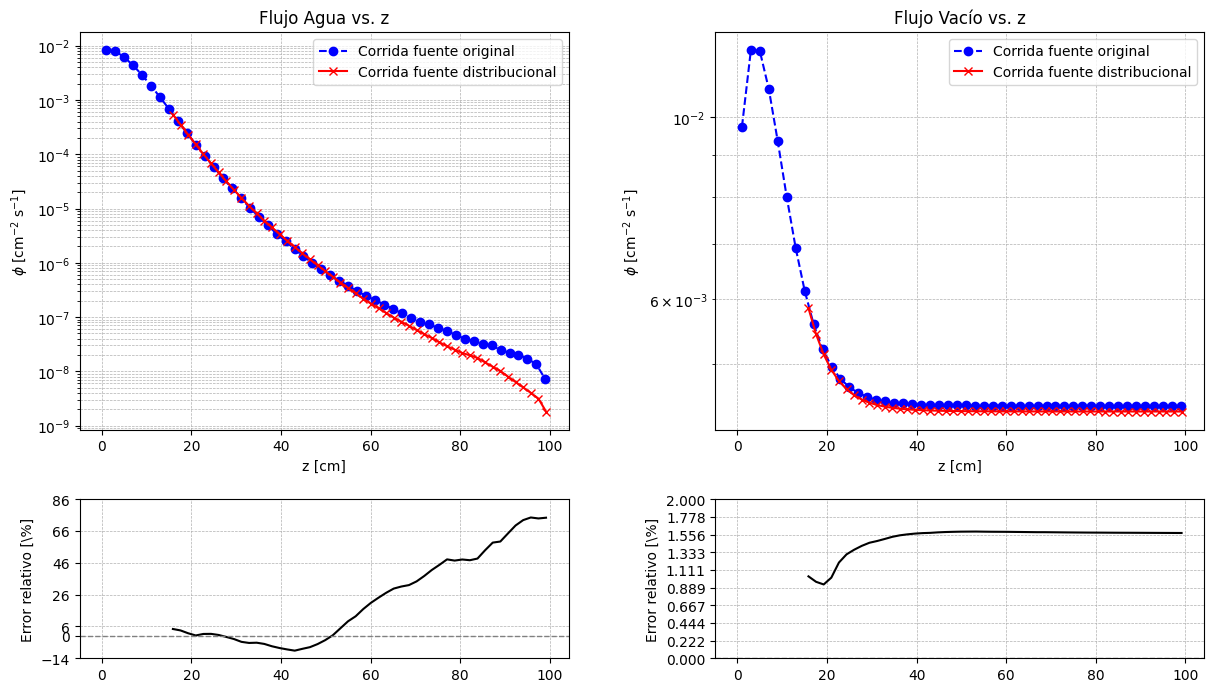
\includegraphics[width=\textwidth]{flujo_1.png}
%     \caption{Comparación entre los perfiles de flujo escalar obtenidos mediante la fuente original (simulación larga desde el inicio del conducto) y mediante la fuente distribucional (simulación desde la superficie intermedia). A la izquierda: región de agua; a la derecha: canal de vacío. En ambos casos se muestra el error relativo.}
%     \label{fig:flujo_comparacion}
% \end{figure}

En la región de agua (Figura \ref{fig:flujo_agua}), se observa un error relativo que no converge con la distancia al origen de la fuente. Este comportamiento se explica por la escasa densidad de peso estadístico presente originalmente en esta región del archivo de partículas original (ver Tabla~\ref{tab:particulas_pesos}), lo cual dificultó la reconstrucción adecuada de su distribución.

En cambio, en el canal de vacío (Figura \ref{fig:flujo_vacio}), se logra una reconstrucción de mayor precisión del perfil original. El error relativo se mantiene por debajo del 1\% en todo el tramo analizado, lo que indica una adecuada correspondencia entre la fuente generada y el perfil de referencia. Cabe destacar que parte del error observado se debe a diferencias entre las distribuciones de corriente presentes en el archivo de partículas original —limitado en estadística— y la simulación larga de referencia. No obstante, las formas del perfil en ambas simulaciones muestran concordancia, validando el enfoque implementado.

\subsection{Comparación del espectro en la salida del canal}

Además del perfil de flujo, se analizó el espectro registrado en la superficie ubicada a $z = 80$~cm. En ambas simulaciones —la original desde el inicio del conducto y la simulación utilizando la fuente distribucional— se registró el espectro de neutrones incidentes sobre dicha superficie. La Figura \ref{fig:espectro_comparacion} muestra los espectros normalizados por neutrón de fuente obtenidos para ambas simulaciones. 

En la Figura \ref{fig:espectro_agua}, correspondiente a la región de agua, se observa que el espectro generado por la fuente distribucional presenta una buena aproximación en las regiones de alta letargía, donde se encuentran los neutrones termalizados. El error relativo en esa zona es bajo, lo que indica que la fuente remuestreada logró capturar adecuadamente la estructura del espectro original.

En la Figura \ref{fig:espectro_vacio} se observa una correcta aproximación en la región de letargía correspondiente a $E = 1~MeV$, donde el error relativo es muy bajo. Esto indica que el remuestreo de los neutrones colimados que se propagan por el canal de vacío se realizó correctamente. Este resultado está en concordancia con lo observado previamente en el perfil de flujo en dicha región (ver Figura \ref{fig:flujo_vacio}), donde el error se mantuvo por debajo del 1\%. En cambio para regiones de mayor letargía, correspondientes a neutrones que han colisionado y se propagan por la región de vacío, se observa un error relativo mayor. 

\begin{figure}[H]
    \centering
    \begin{subfigure}[t]{0.48\textwidth}
        \centering
        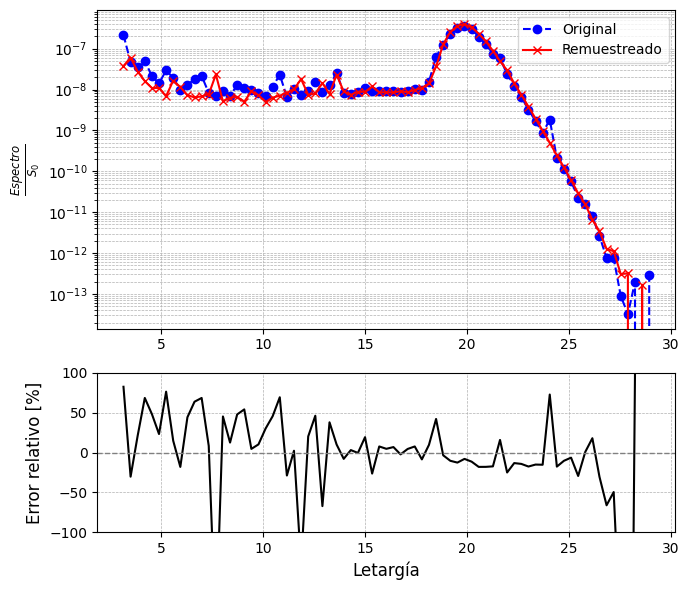
\includegraphics[width=\textwidth]{espectro_agua.png}
        \caption{Región de agua.}
        \label{fig:espectro_agua}
    \end{subfigure}
    \hfill
    \begin{subfigure}[t]{0.48\textwidth}
        \centering
        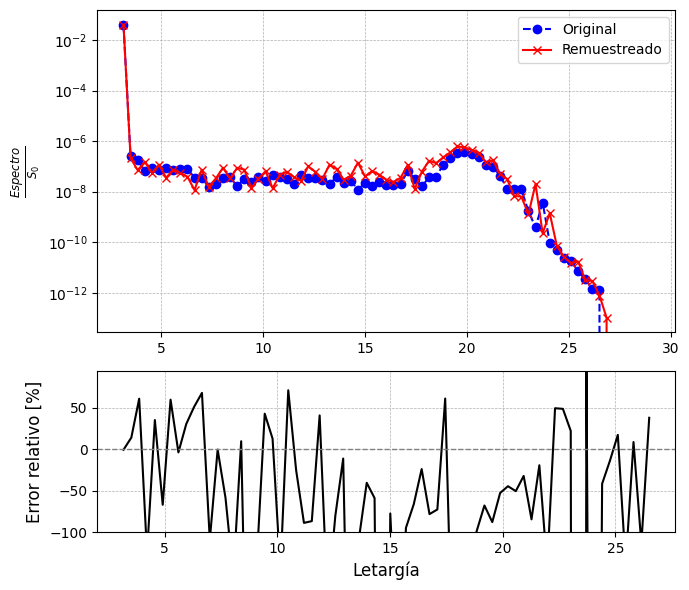
\includegraphics[width=\textwidth]{espectro_vacio.png}
        \caption{Canal de vacío.}
        \label{fig:espectro_vacio}
    \end{subfigure}
    \caption{Comparación del espectro de neutrones en la superficie a $z = 80$~cm para las simulaciones original y remuestreada. En ambos casos se incluye también el error relativo porcentual.}
    \label{fig:espectro_comparacion}
\end{figure}


% En cambio, para regiones de mayor letargía, correspondientes a neutrones presentes en el agua, se observa una subestimación en el espectro generado por la fuente distribucional. Este efecto se explica por la baja estadística disponible originalmente en el agua, lo que dificultó capturar adecuadamente dicha contribución. Tal como se mencionó en la sección anterior, el perfil de flujo en la región de agua mostró una atenuación progresiva con la distancia (ver Figura \ref{fig:flujo_comparacion}, izquierda), fenómeno que se reproduce aquí en forma espectral.

% A pesar de esta diferencia en magnitud, se destaca que la forma general del espectro se mantiene coherente entre ambas simulaciones. Esto sugiere que, si bien el contenido total en la región del agua fue subrepresentado, el método logró capturar correctamente la estructura cualitativa del espectro original.

\subsection{Comparación de la corriente}

Se analizó la corriente total de neutrones atravesando la superficie ubicada a $z = 80$~cm para ambas simulaciones. En la simulación original, ejecutada desde el inicio del canal con alta estadística, se obtuvo una corriente normalizada de
\[
J_{\text{original}} = (4.005 \pm 0.003) \times 10^{-2} \; \text{neutrones por neutrón fuente}.
\]

Por otro lado, la simulación realizada con la fuente remuestreada arrojó un valor de
\[
J_{\text{remuestreada}} = (4.037 \pm 0.008) \times 10^{-2} \; \text{neutrones por neutrón fuente}.
\]

Esto representa un 100.8\% del valor original, lo cual indica una aceptable conservación de la corriente total. 


\section{Conclusiones preliminares}

El estudio aplicado al caso de un canal de vacío rodeado por agua permitió evaluar el desempeño del método de generación de fuentes distribucionales basado en histogramas multidimensionales. Este caso representa una situación física relevante y sensible, ya que involucra la coexistencia de poblaciones de neutrones con comportamientos distintos: una colimada y monoenergética en el vacío, y otra dispersa y moderada en el agua.

Los principales resultados obtenidos son:

\begin{itemize}
    \item Se logró reconstruir el flujo escalar y el espectro en el canal de vacío. La región colimada de neutrones sin colisiones fue correctamente representada por el método propuesto.
    
    % \item La reconstrucción del flujo y el espectro en el agua presentó limitaciones más marcadas, debidas a la poca estadistica en el agua en el archivo de particulas original.

    \item Se observó que el uso de histogramas adaptativos permite una representación más equilibrada y autónoma del espacio de fases, sin necesidad de intervención manual. No obstante, la incorporación de bordes definidos por el usuario sigue siendo una herramienta útil cuando se dispone de información a priori sobre el sistema, especialmente para evitar mezclas artificiales entre poblaciones diferenciadas.

    \item La implementación de una reducción progresiva en la resolución de los histogramas macro y micro resultó eficaz para evitar el sobreajuste en conjuntos de poca estadística, evitando amplificar el ruido estadístico.
\end{itemize}

% Sin embargo, es importante destacar que la calidad de la fuente generada depende de la calidad estadística del archivo de partículas original. Este punto se discute en mayor profundidad en el Apéndice \ref{app:B}, donde se analiza el mismo caso utilizando un archivo de partículas con mayor estadística. En dicho análisis se obtienen mejoras significativas en la reconstrucción de la región de agua.



\chapter{Validación experimental: Conducto Nº5 del reactor RA-6}
% \label{chap:validacion-ra6}

El presente capítulo se validará el método de remuestreo de partículas mediante histogramas multidimensionales desarrollado en este trabajo. Para ello, se lo aplicará al conducto Nº5 del reactor RA-6, un reactor nuclear de investigación tipo pileta ubicado en el Centro Atómico Bariloche (CAB), Argentina.

El RA-6 cuenta con 5 conductos de extracción de neutrones diseñados para transportar haces desde el núcleo hacia diferentes instalaciones experimentales. En particular, el Departamento de Neutrones del CAB ha desarrollado espectrometría basada en la técnica de tiempo de vuelo (TdV) sobre el conducto Nº5. Esto se realiza utilizando un instrumento denominado \textit{chopper}, cuya función es pulsar el haz de neutrones. Midiendo el tiempo que tardan los neutrones en viajar desde el \textit{chopper} hasta un banco de detectores de \textsuperscript{3}He, se obtiene el espectro de energía del haz mediante TdV.

A su vez, el Departamento de Neutrones ha realizado simulaciones Monte Carlo del RA-6 utilizando el código \texttt{OpenMC} con el objetivo de estimar la distribución espectral en el banco de detectores. Sin embargo, debido a la baja probabilidad de que un neutrón simulado desde el núcleo alcance dicha región, una simulación directa resulta computacionalmente inviable.

Para superar esta limitación, se empleó una segmentación geométrica del problema. En una primera simulación desde núcleo, el Departamento de Neutrones registró un archivo de partículas en la entrada del conducto Nº5. Con este archivo de partículas se generó una fuente distribucional con el método de histogramas multidimensionales. Esta fuente se utilizó como entrada en una segunda simulación de \texttt{OpenMC}, que modela exclusivamente el conducto Nº5 hasta el banco de detectores.

Este enfoque permite generar una mayor cantidad de partículas en la entrada del conducto Nº5 de las que se registró originalmente en el archivo de partículas. Esto permite incrementar la estadística en los detectores sin necesidad de simular desde el núcleo. 

De este modo, se posibilita una comparación entre los resultados obtenidos aplicando el metodo de remuestreo utilizando histogramas multidimensionales y las mediciones experimentales realizadas por el Departamento de Neutrones, permitiendo validar el método implementado.

En las secciones siguientes se describen la geometría del reactor y del conducto Nº5, y los resultados obtenidos de flujo neutrónico y espectro de energía.

\section{Descripción del reactor RA-6 y instalación experimental del conducto Nº5}

El núcleo del reactor RA-6 está compuesto por 20 elementos combustibles del tipo placa de aluminio \textit{meat} de siliciuro de uranio enriquecido al 19,70\%. Este conjunto, cuya altura activa alcanza los 70,5~cm, se encuentra sumergido en una pileta de agua liviana que actúa simultáneamente como moderador, refrigerante, reflector axial y blindaje biológico. Lateralmente, el reflector está constituido por bloques de grafito. El núcleo opera a una potencia de 1~MW térmico y está alojado en una pileta cilíndrica de 2,4~m de diámetro, rodeada a su vez por un blindaje biológico de hormigón pesado con forma octogonal. En la Figura \ref{fig:esquema-nucleo} se presenta un esquema representativo del núcleo y sus alrededores.

\begin{figure}[h]
\centering
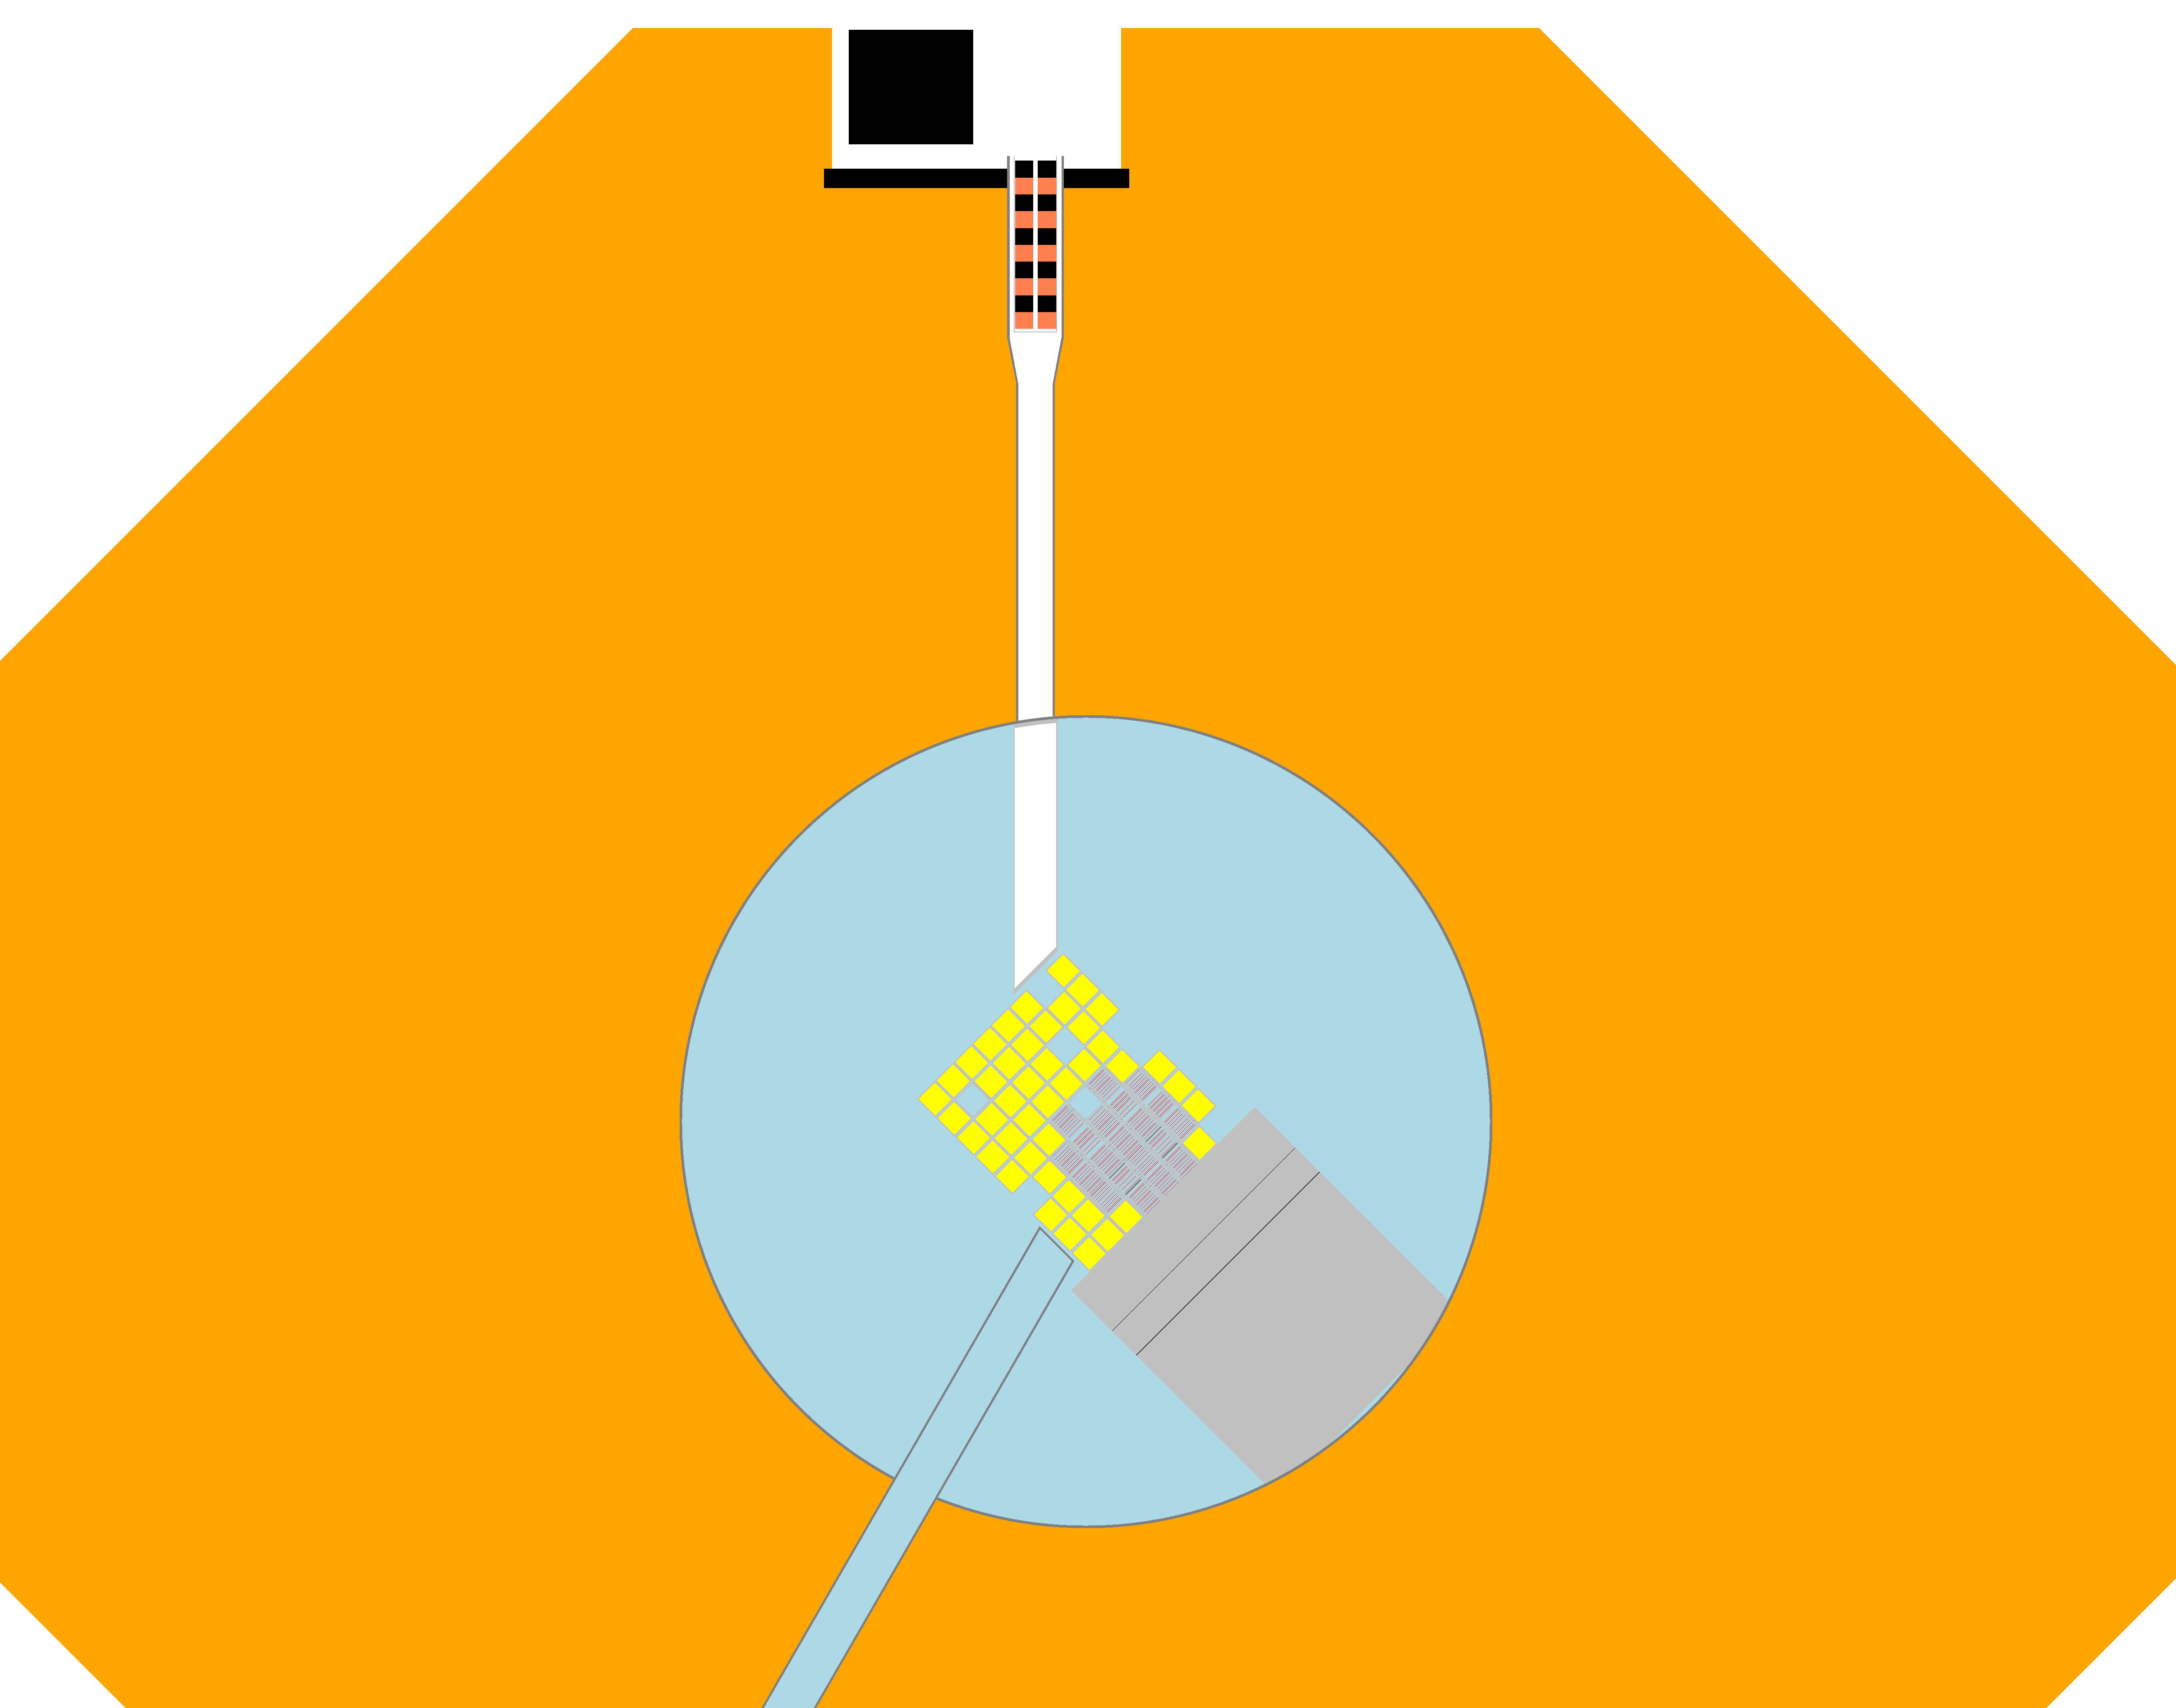
\includegraphics[width=0.75\textwidth]{ra6.png}
\caption{Esquema representativo del núcleo del RA-6. En el mismo se observa la disposición de los elementos combustibles, el conducto Nº1 (inferior) y el conducto Nº5 (superior) \cite{DeptoNeutronesCAB2025}.}
\label{fig:esquema-nucleo}
\end{figure}

El reactor cuenta con cinco conductos de extracción de neutrones destinados a experimentación. En la Figura~\ref{fig:esquema-nucleo} se destacan dos de ellos: el conducto Nº1 y el conducto Nº5. En particular, el conducto Nº5 se orienta hacia una zona del núcleo en la que se encuentran ubicadas un bloque de grafito y un bloque de agua. Dado que no apunta directamente hacia los elementos combustibles, el espectro resultante en este canal está compuesto mayoritariamente por neutrones térmicos.

El conducto Nº5 consiste en un cilindro de acero de 5cm de radio, que atraviesa la pileta del reactor y el blindaje biológico. En su interior se encuentra un colimador constituido por secciones alternadas de plomo y parafina borada. Además, las dos primeras secciones del colimador contienen un filtro de bismuto, utilizado para atenuar la componente de radiación $\gamma$ del haz. Esta atenuación resulta fundamental en experimentos, ya que permite reducir el fondo de radiación $\gamma$ que puede saturar los detectores utilizados. La Figura \ref{fig:conducto} muestra un esquema detallado del conducto Nº5 y de su sistema de colimación, como así también el banco de detectores utilizados en la medición experimental.

\begin{figure}[h]
\centering
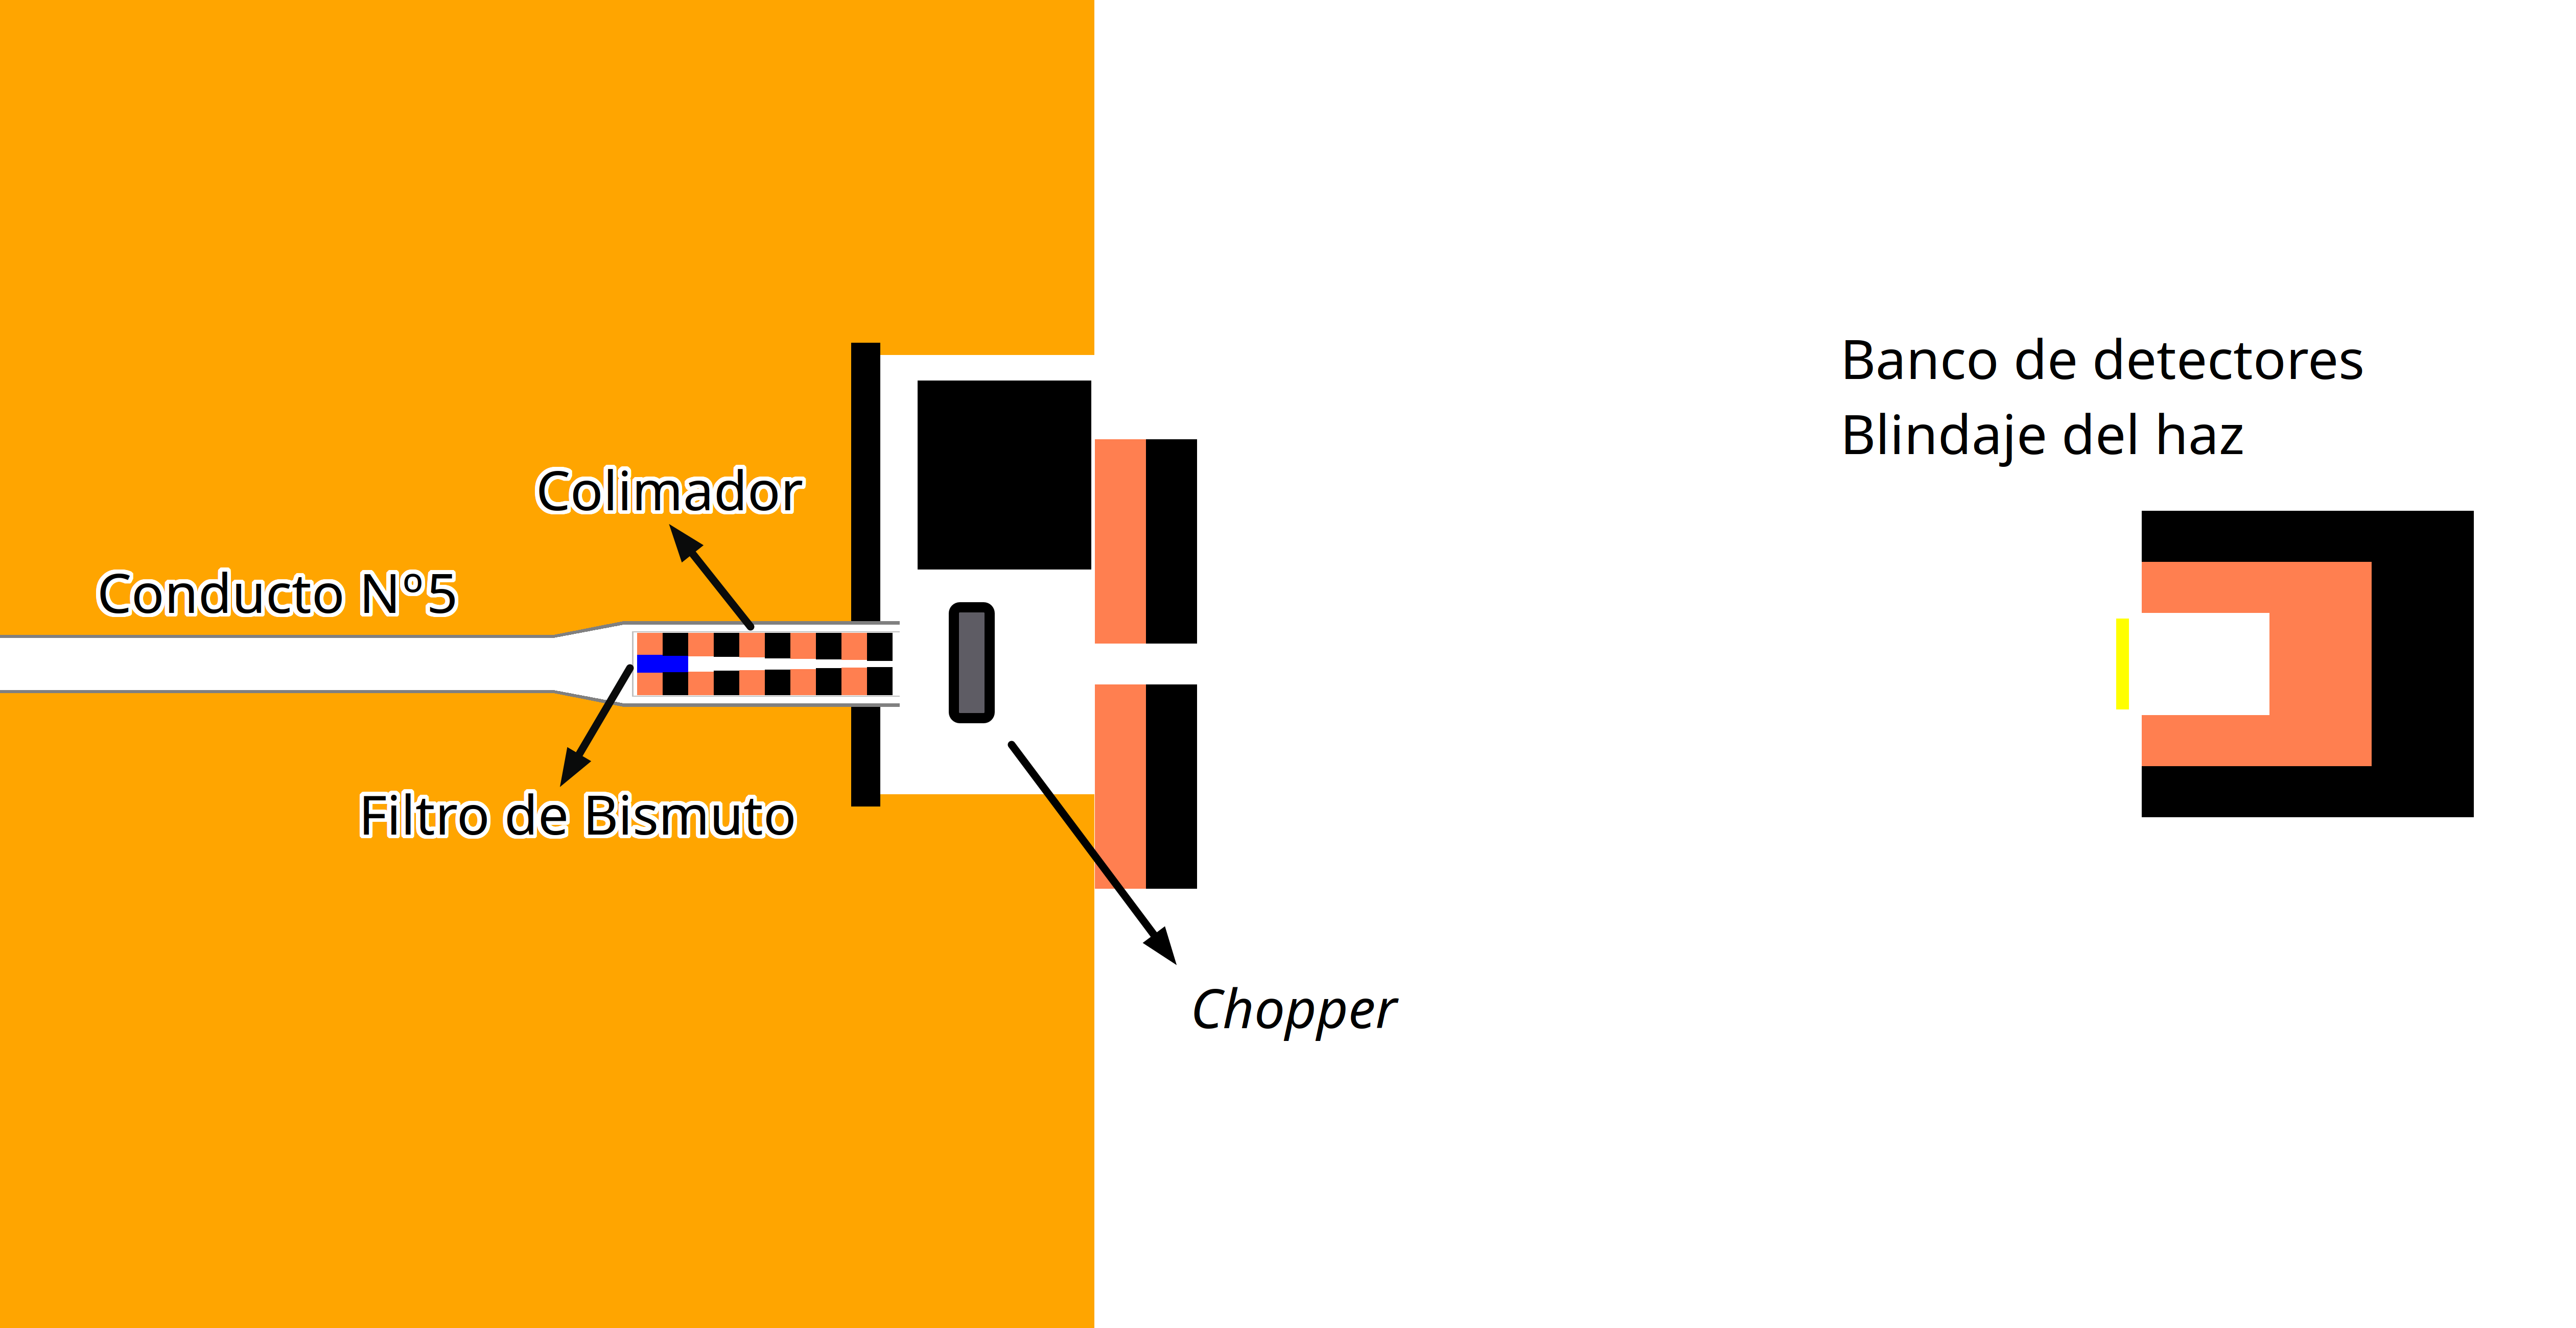
\includegraphics[width=0.9\textwidth]{conducto.png}
\caption{Esquema representativo del conducto Nº5 del RA-6 y de la instalación experimental asociada al \textit{chopper} \cite{DeptoNeutronesCAB2025}.}
\label{fig:conducto}
\end{figure}

Este conducto está asociado a un intrumento experimental denominado \textit{chopper}, diseñada para la generación de haces pulsados de neutrones. El dispositivo \textit{chopper} consiste en un disco rotatorio de material absorbente con una ranura, el cual se posiciona a la salida del conducto. Al girar a velocidad constante, la ranura permite periódicamente el paso de neutrones cuando se encuentra alineada con el eje del haz. De esta manera, se obtienen pulsos neutrónicos que pueden ser utilizados para realizar espectrometría mediante la técnica de tiempo de vuelo (TdV). La Figura \ref{fig:chopper} ilustra esquemáticamente el mecanismo de funcionamiento del disco \textit{chopper}.

\begin{figure}[h]
\centering
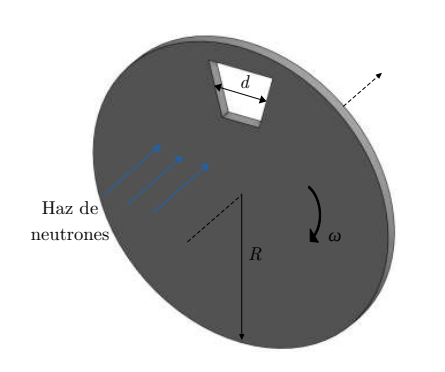
\includegraphics[width=0.5\textwidth]{DISCO_CHOPPER.png}
\caption{Esquema representativo del disco rotatorio del \textit{chopper} empleado en el conducto Nº5. La ranura permite el paso periódico de neutrones, generando un haz pulsado \cite{DeptoNeutronesCAB2025}.}
\label{fig:chopper}
\end{figure}

Para la implementación experimental de esta técnica, se dispone un banco de cinco detectores de \textsuperscript{3}He a una distancia conocida de la salida del conducto. Estos detectores registran el tiempo de llegada de cada neutrón, a partir del cual se calcula su energía cinética mediante la expresión:

\begin{equation}
E = \frac{1}{2} m_n v^2,
\end{equation}

donde $E$ es la energía del neutrón, $m_n$ su masa, y $v$ la velocidad obtenida como el cociente entre la distancia conocida y el tiempo medido.

Para reconstruir correctamente el espectro neutrónico, es necesario corregir la señal detectada. En primer lugar, se debe restar un fondo constante asociado a la componente gamma y a neutrones que atraviesan el \textit{chopper} fuera de fase. Adicionalmente, se aplican correcciones por el tiempo muerto del sistema de adquisición de datos y por la eficiencia de detección de los tubos de \textsuperscript{3}He.

Finalmente, detrás del banco de detectores se instala un blindaje adicional que permite blindar el haz y proteger las áreas experimentales circundantes.

\section{Procesamiento del archivo de partículas}

% El departamento de neutrones del CAB ha proporcionado un archivo de partículas que contiene información sobre las trayectorias de los neutrones que ingresan al conducto N5. Este archivo surge de una simulacion desde nucleo del RA-6 en OpenMC. Esta simulacion consto de 1e10 particulas, y se registro un archivo de particulas que contenia 41245 particulas que ingresaron al conducto N5. Sin embargo como estas particulas provienen de una simulacion con esquema de reduccion de varianza incorporado, algunas de estas particulas tienen un peso menor a 1. Por lo tanto, en el archivo de particulas original se cuenta con un total de 22182 de peso estadistico, sumando todas las particulas. 

% En la figura tal se presenta la distribucion en el plano XY de las particulas. Estas forman un circulo de radio $5,\text{cm}$, que corresponde al radio del conducto. Se observa que las particulas se distribuyen uniformemente en el circulo.

% \begin{figure}[h]
%     \centering
%     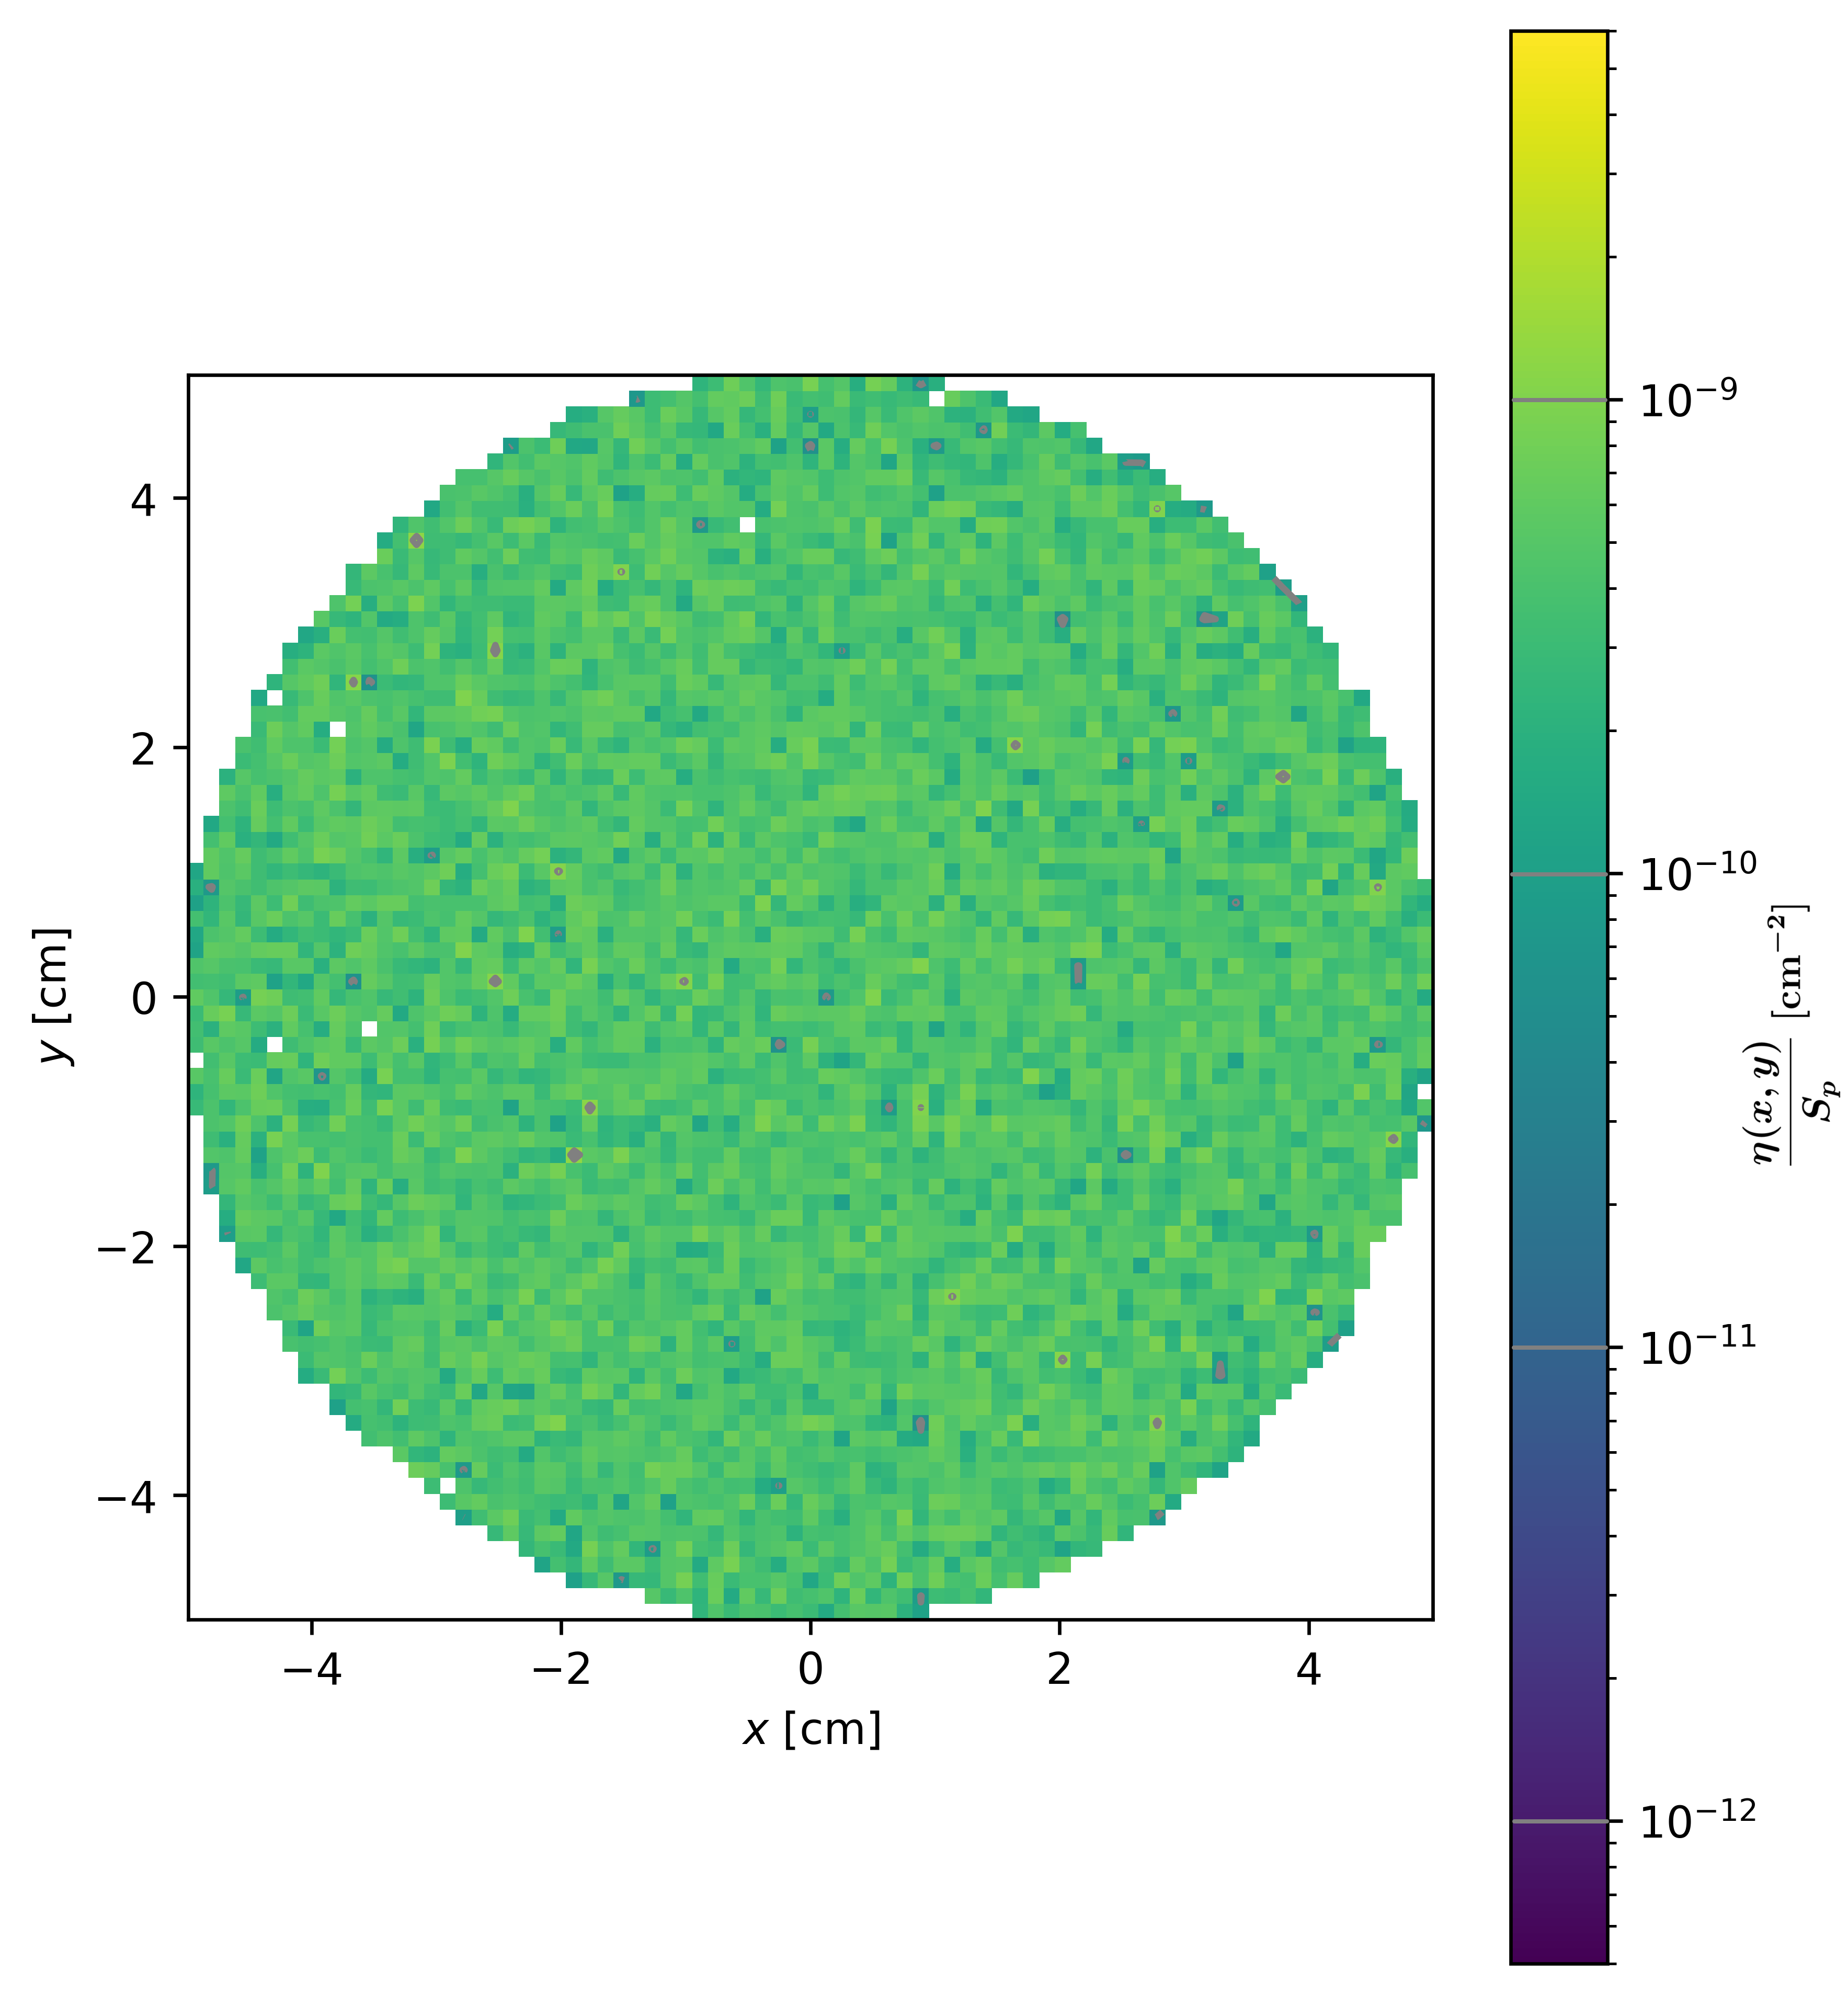
\includegraphics[width=0.75\textwidth]{conducto_XY.png}
%     \caption{Distribución espacial de las partículas del archivo original en el plano XY.}
%     \label{fig:conducto-XY}
% \end{figure}

% En la figura tal se presenta la distribucion de letargia de las particulas del archivo original. Se observa que las mismas presentan una acumulacion sobre la region de fision alrededor de $ln(E_0/E) = 2$, donde $E_0 = 20 MeV$ y otra acumulacion de mayor proporsion en la region de termalizacion alrededor de $ln(E_0/E) = 19$.

% \begin{figure}[h]
%     \centering
%     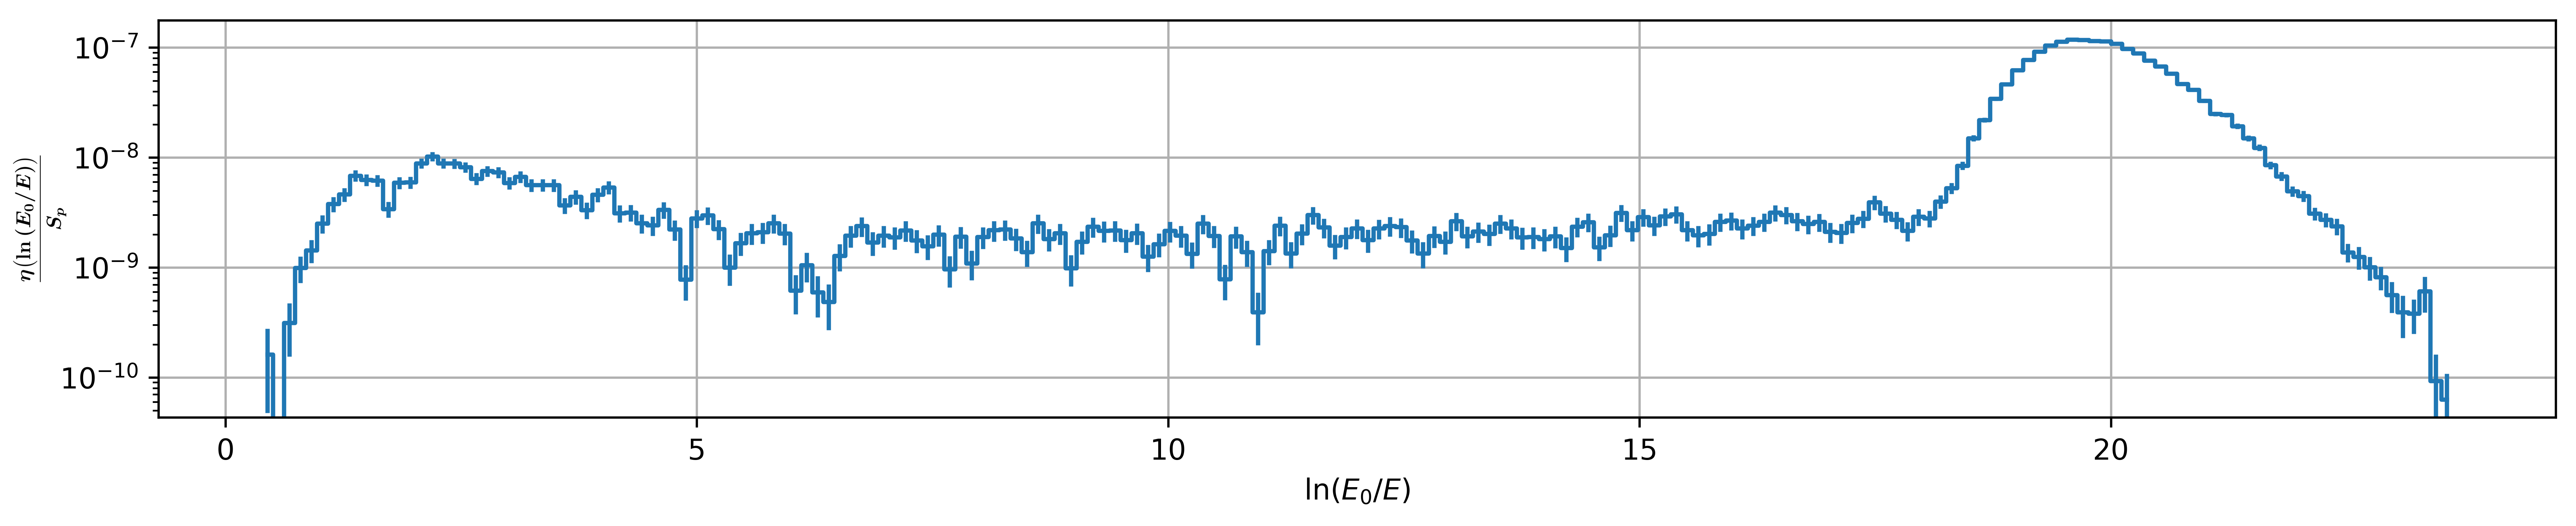
\includegraphics[width=\textwidth]{conducto_let.png}
%     \caption{Distribución de letargía de las partículas del archivo original.}
%     \label{fig:conducto-let}
% \end{figure}

% Para generar la fuente distribucional, se emplea el método de histogramas multidimensionales desarrollado en este trabajo. La configuracion utilizada fue:


% \begin{itemize}
%     \item Orden de procesamiento: \texttt{[letargía, X, Y, $\mu$, $\phi$]}
%     \item Número de histogramas macro: [3, 7, 4, 4]
%     \item Número de histogramas micro: [75, 18, 18, 15, 10]
% \end{itemize}

% Se decidio brindarle mayor resolucion a la letargia, ya que es la variable de mayor interes en este caso y es necesario obtener una buena resolucion en la zona de termalizacion, debido a que el objetivo de este capitulo es comparar el espectro termico medido a traves de la tecnica de TdV. 

% A su vez se decidio brindarle la mayor cantidad de bines al histograma macro de la variable $X$ para obtener una mejor representacion del circulo. En caso de tomar menos bines para la variable $X$ se observaria patrones debidos a la discretizacion del histograma macro.

% Con esta fuente distribucional se procede a comparar el resultado obtenido de las distribuciones de letargia y posicion XY de las particulas. En la figura tal se presenta la distribucion en el plano XY de las particulas generadas por la fuente distribucional. A comparacion con la otra figura se observa que se logra representativomente el circulo de radio $5,\text{cm}$, aunque sin embargo se pueden apreciar los bordes debidos a la discretizacion con histogramas macro aplicada.

% \begin{figure}[h]
%     \centering
%     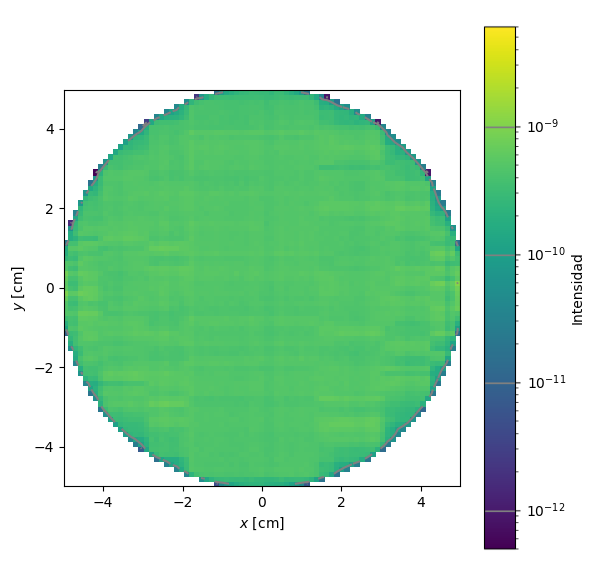
\includegraphics[width=0.75\textwidth]{conducto_comparacion_XY.png}
%     \caption{Distribución espacial de las partículas de la fuente distribucional en el plano XY.}
%     \label{fig:conducto-comparacion-XY}
% \end{figure}

% En la figura tal se presenta la comparacion de la distribucion de letargia de las particulas del archivo original y las generadas por la fuente distribucional. Se observa la mayor resolucion en el histograma de letargia, para poder obtener una aproximacion de mejor resolucion en la zona de termalizacion, a costa de reproducir el ruido estadistico en la zona epitermica.

% \begin{figure}[h]
%     \centering
%     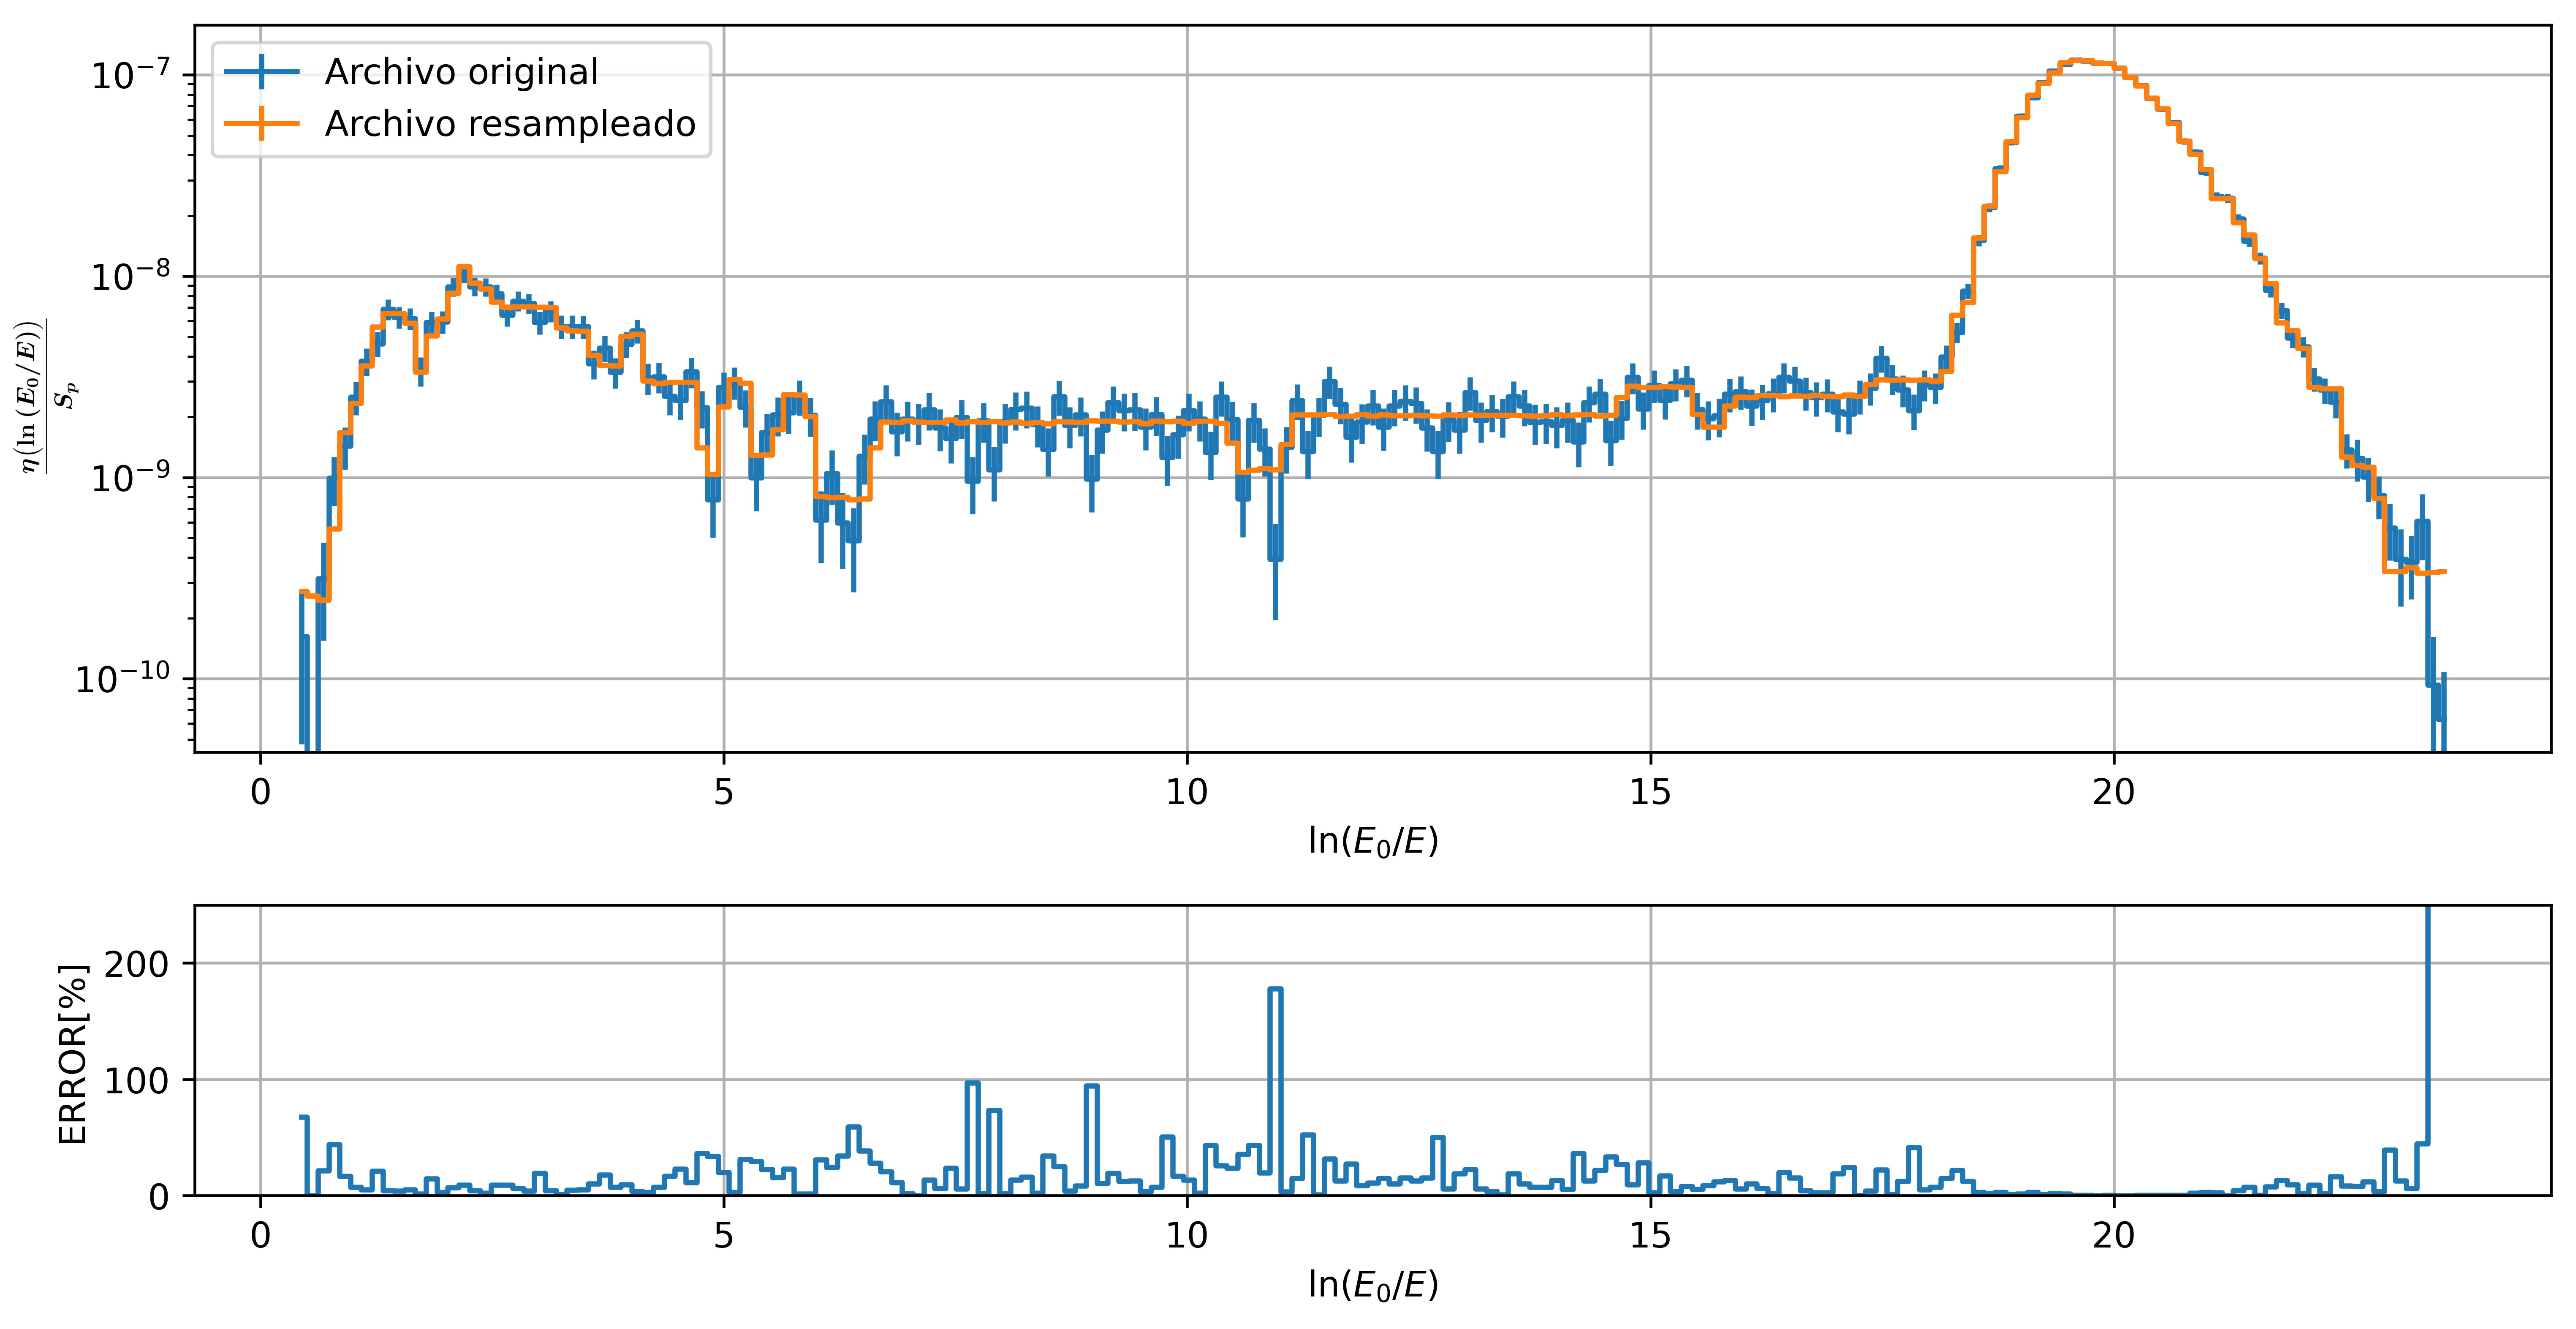
\includegraphics[width=\textwidth]{conducto_comparacion_let.png}
%     \caption{Comparación de la distribución de letargia entre el archivo original y la fuente distribucional.}
%     \label{fig:conducto-comparacion-let}
% \end{figure}

El Departamento de Neutrones del Centro Atómico Bariloche proporcionó un archivo de partículas que contiene información sobre los neutrones que ingresan al conducto Nº5. Este archivo fue generado a partir de una simulación del núcleo completo del reactor RA-6 utilizando el código \texttt{OpenMC}. La simulación consistió en un total de $10^{10}$ partículas fuente, de las cuales 41245 fueron registradas en la entrada del conducto Nº5.

Cabe destacar que esta simulación fue realizada con un esquema de reducción de varianza, lo que implica que muchas partículas del archivo presentan un peso estadístico menor a la unidad. La suma total de los pesos estadísticos de las partículas registradas fue 22182.

En la Figura~\ref{fig:conducto-XY} se muestra la distribución espacial de las partículas registradas en el plano $XY$. Puede observarse que las posiciones conforman un círculo de radio 5~cm, correspondiente a la sección transversal del conducto Nº5. La distribución es aproximadamente uniforme dentro del círculo.

\begin{figure}[h]
\centering
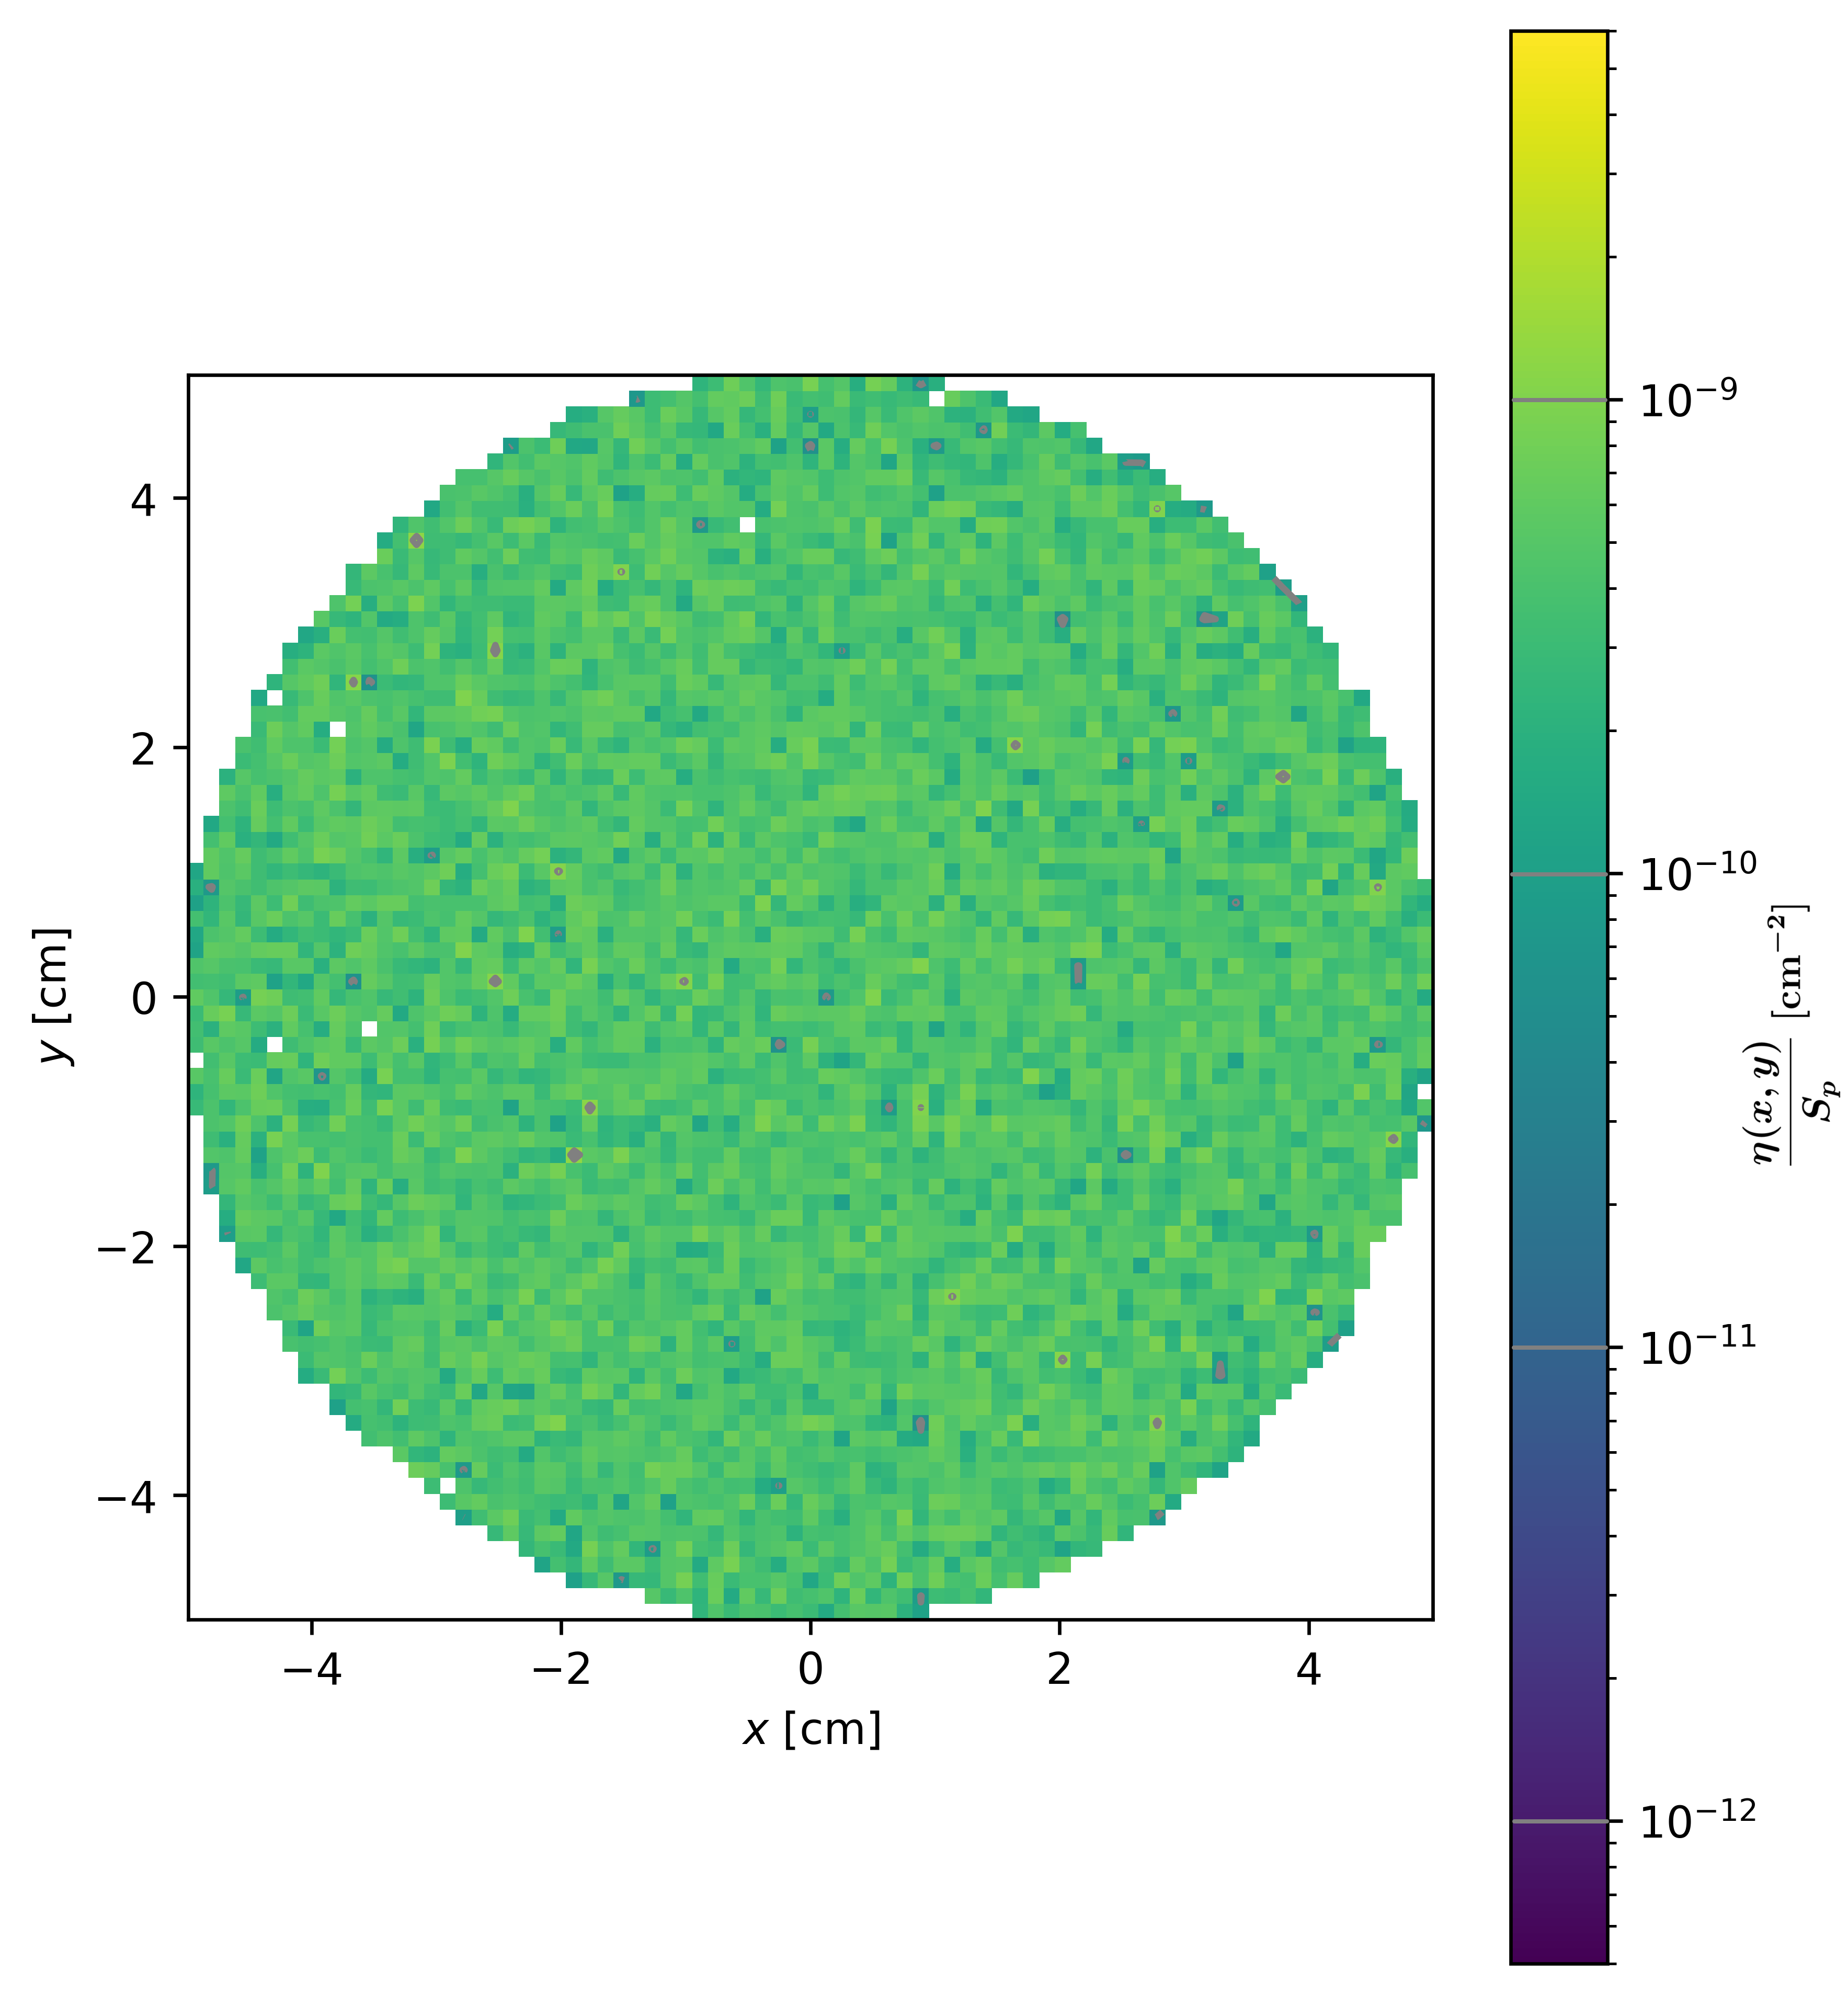
\includegraphics[width=0.75\textwidth]{conducto_XY.png}
\caption{Distribución espacial de las partículas del archivo original en el plano $XY$.}
\label{fig:conducto-XY}
\end{figure}

La Figura~\ref{fig:conducto-let} presenta la distribución de letargía de las partículas registradas. Se observan dos regiones de acumulación: una alrededor de $\ln(E_0/E) \approx 2$, correspondiente a energías típicas de fisión, y otra de mayor intensidad en la región térmica, centrada en $\ln(E_0/E) \approx 19$, donde $E_0 = 20$~MeV.

\begin{figure}[h]
\centering
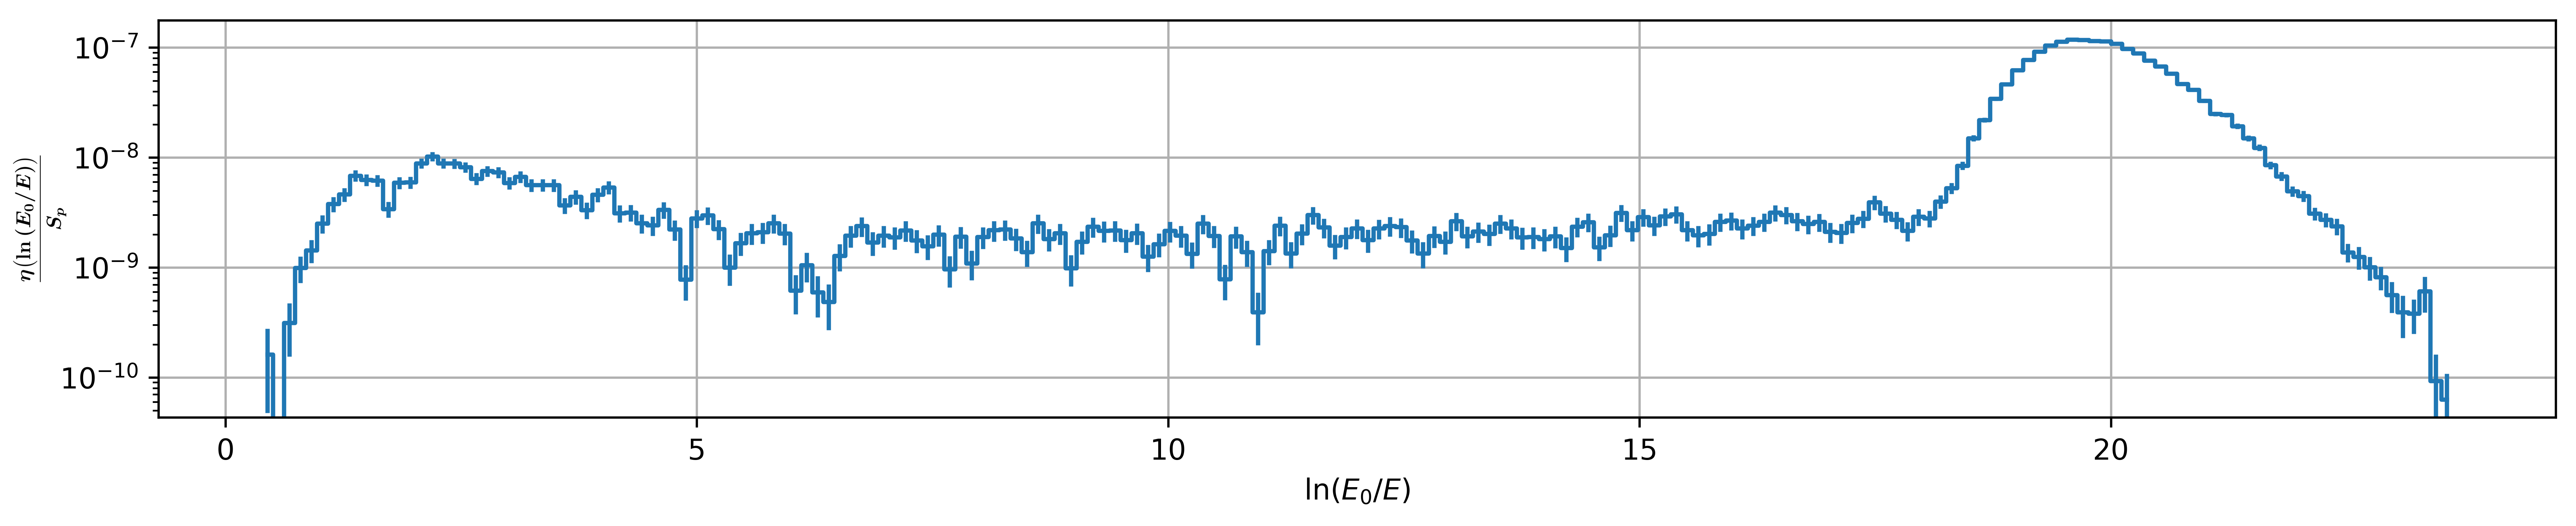
\includegraphics[width=\textwidth]{conducto_let.png}
\caption{Distribución de letargía de las partículas del archivo original.}
\label{fig:conducto-let}
\end{figure}

A partir de este archivo de partículas, se generó una fuente distribucional mediante el método de histogramas multidimensionales desarrollado en este trabajo. La configuración adoptada para la construcción de la fuente distribucional fue la siguiente:

\begin{itemize}
\item \textbf{Orden de procesamiento}: \texttt{[letargía, X, Y, $\mu$, $\phi$]}
\item \textbf{Número de histogramas macro}: \texttt{[3, 7, 4, 4]}
\item \textbf{Número de histogramas micro}: \texttt{[75, 18, 18, 15, 10]}
\end{itemize}

Se asignó una mayor resolución a la variable letargía, dado que constituye el objetivo principal de análisis en este capítulo, centrado en la comparación espectral mediante la técnica de tiempo de vuelo. Además, se destinó una mayor cantidad de divisiones macro a la coordenada $X$ para mejorar la representación del contorno circular del conducto. Se verificó que al reducir la resolución en dicha coordenada, aparecían patrones discretos artificiales en el plano $XY$, producto de una segmentación insuficiente del dominio espacial.

La Figura~\ref{fig:conducto-comparacion-XY} muestra la distribución en el plano $XY$ de las partículas generadas por la fuente distribucional. Puede observarse que la forma circular de radio 5~cm se reproduce adecuadamente, aunque la discretización asociada a los histogramas macro introduce estructuras visibles en los bordes.

\begin{figure}[h]
\centering
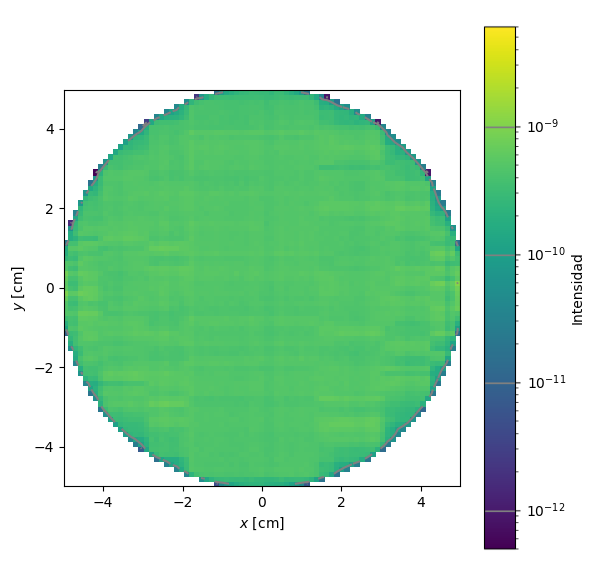
\includegraphics[width=0.75\textwidth]{conducto_comparacion_XY.png}
\caption{Distribución espacial de las partículas de la fuente distribucional en el plano $XY$.}
\label{fig:conducto-comparacion-XY}
\end{figure}

En la Figura~\ref{fig:conducto-comparacion-let} se presenta la comparación entre la distribución de letargía del archivo original y la correspondiente a la fuente generada. La mayor resolución elegida para el eje de letargía permite representar en detalle la zona térmica, a costa de reproducir parte del ruido estadístico presente en la región epitérmica.

\begin{figure}[h]
\centering
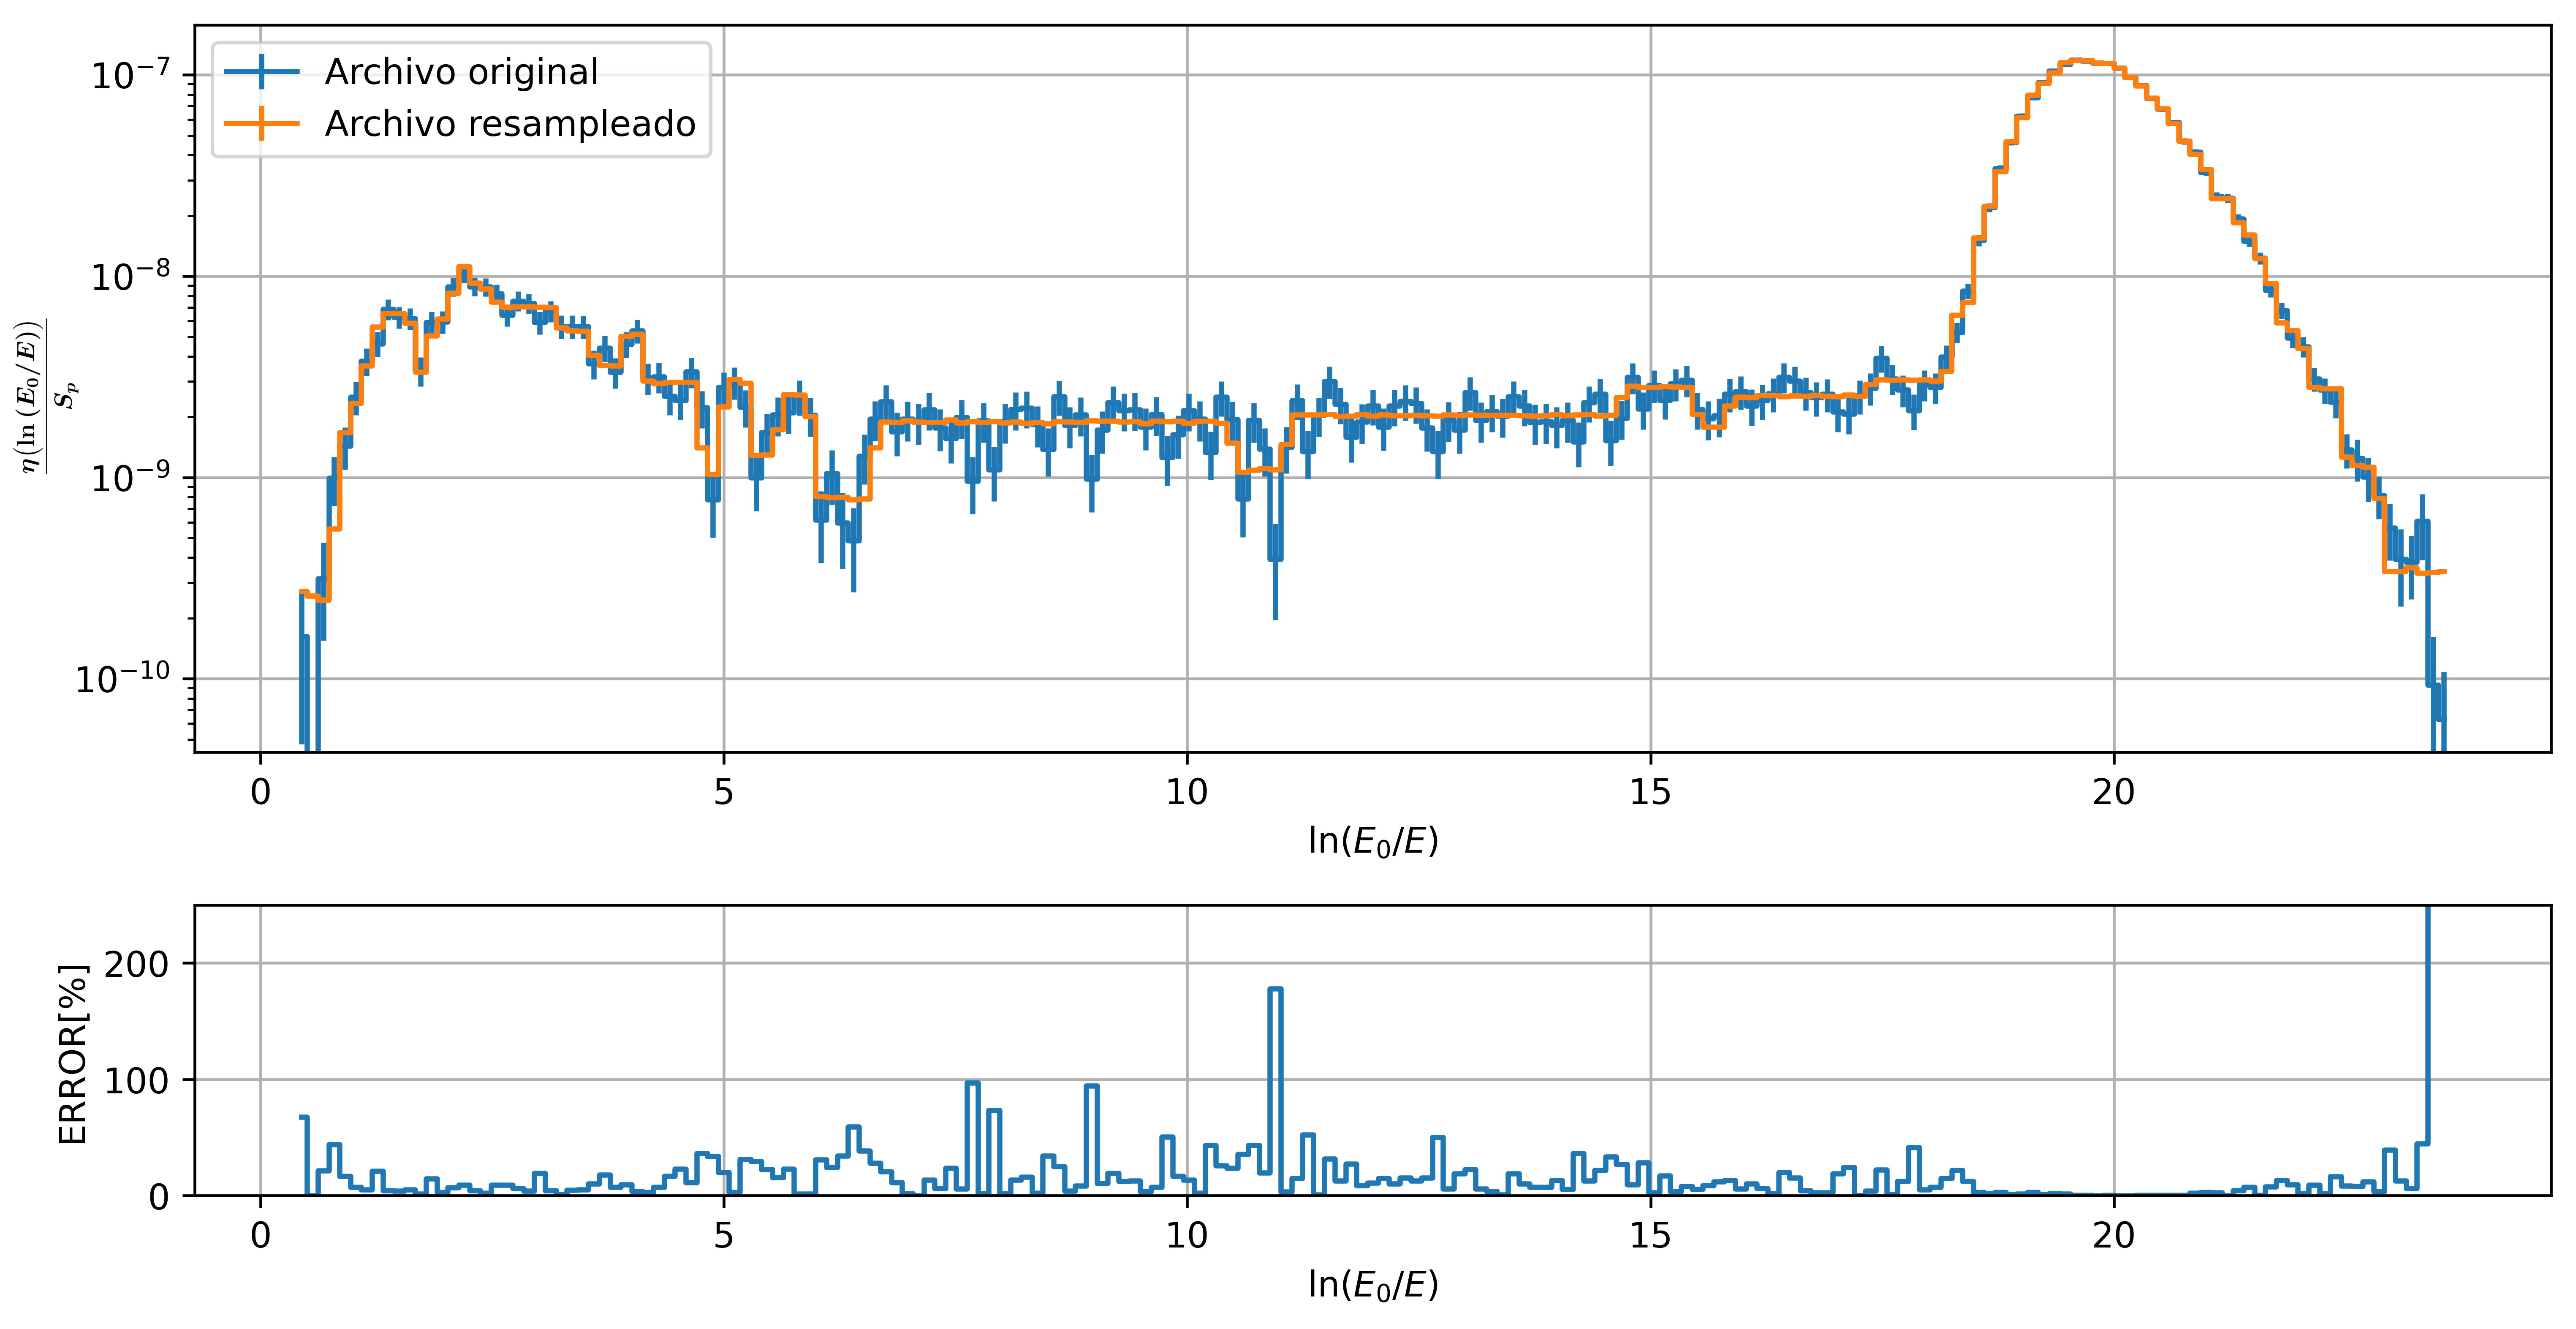
\includegraphics[width=\textwidth]{conducto_comparacion_let.png}
\caption{Comparación de la distribución de letargía entre el archivo original y la fuente distribucional.}
\label{fig:conducto-comparacion-let}
\end{figure}

% \label{sec:optimizacion-w}

\section{Resultados de simulación en \texttt{OpenMC} y comparación experimental}
% \label{sec:resultados-w}

% A partir de la fuente distribucional generada, se procedio a hacer una segunda simiulacion del conducto N5, esta vez utilizando la fuente generada por el método de remuestreo. Esta simulacion consto de 5e9 particulas. Para aumentar la estadistica se utilizo un esqeuam de reduccion de varianza de tipo sesgo de supervivencia, que permite aumentar la probabilidad de que las particulas lleguen al banco de detectores.

% En esta simulacion se registro el flujo neutronico en todo el modelo y se registro el espectro neutronico obtenido en el banco de detectores. Este espectro neutronico se comparo contra el espectro medido experimentalmente en el N5 por tecnica de TdV. 

% \subsection{Distribución espacial del flujo}
% En la figura tal se presenta el flujo neutronico obtenido en el modelo implementado del conducto N5. Se observa que se ha adquirido un flujo converjido en la zona del banco de detectores. Tambien es posible observar que el flujo decae varios ordenes de magnitud al atravesar el conducto y el colimador. Esto evidencia la necesidad de desacoplar la simulacion del conducto del núcleo del reactor, debido a que la probabilidad de que los neutrones lleguen al banco de detectores es muy baja. Por lo tanto en caso de simular desde el nucleo se obtendria que la probabilidad de que lleguen del nucleo al conducto es baja y habria que juntar eso con la probabilidad de que los neutrones atraviesen el colimador y lleguen al banco de detectores, lo que haria que la estadistica en el banco de detectores sea muy baja. En cambio, al desacoplar la simulacion del conducto del nucleo, se logra obtener una estadistica mucho mayor en el banco de detectores, ya que se simula directamente desde la fuente distribucional.

% \begin{figure}[h]
%     \centering
%     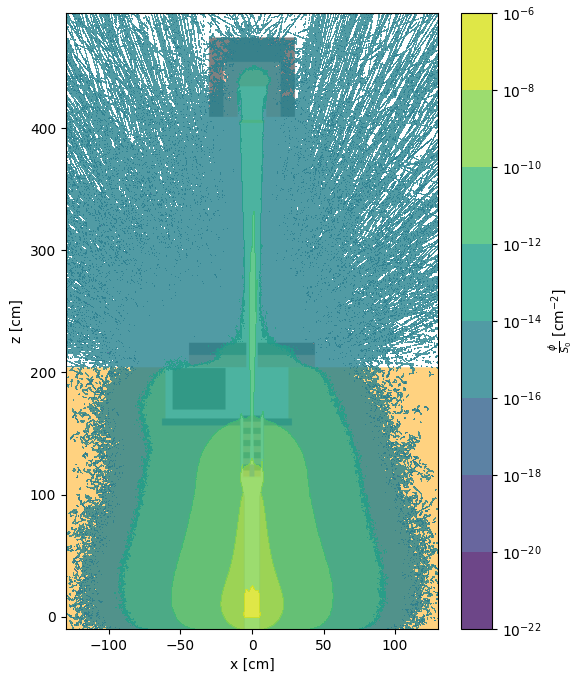
\includegraphics[width=\textwidth]{conducto_flujo.png}
%     \caption{Distribución del flujo neutronico en el modelo del conducto N5.}
%     \label{fig:conducto-flujo}
% \end{figure}

% \subsection{Comparación detector \textsuperscript{3}He}
% En la figura tal se presenta el espectro de neutrones obtenido en el banco de detectores, comparado contra la medicion experimental. Se observa corcordancia entre el espectro medido y el simulado a traves de la fuente distribcuional a partir de los 0.01 eV. Sin embargo, a energias menores a 0.01 eV se observa que el flujo simulado es menor que el medido experimentalmente. 

% \begin{figure}[h]
%     \centering
%     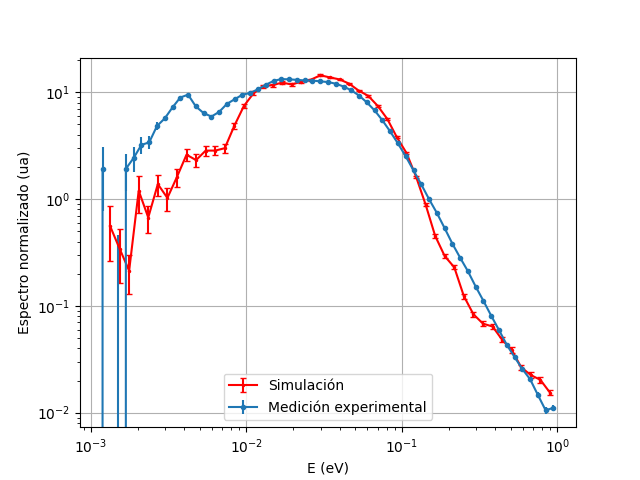
\includegraphics[width=\textwidth]{conducto_espectro.png}
%     \caption{Comparación del espectro de neutrones obtenido en el banco de detectores en la simulación de \texttt{OpenMC} con la medición experimental realizada por TdV por el Departamento de Neutrones del CAB.}
%     \label{fig:conducto-espectro}
% \end{figure}

% Esta discrepancia puede deberse a dos razones:
% \begin{itemize}
%     \item En la figura de la comparacion de letargia se observa que en la zona de mayor letargia se presenta mayor discrepancia entre el espectro del archivo original y el espectro de la fuente distribucional. Esto se debe a que la fuente distribucional no logra reproducir con la misma precision el espectro de letargia del archivo original, debido a la discretizacion en histogramas. Esto provoca que haya mayor discrepancia en la zona de mayor letargia, que corresponde a las energias menores a 0.01 eV.
%     \item La segunda razon esta relacionada al filtro de bismuto. La simulacion en OpenMC utiliza secciones eficaces de bismuto como atomos libres. Sin embargo el filtro utilizado es un cristal, por lo que existen diferencias entre la seccion eficaz a bajas energias. Para energias mayores a 0.1 eV no existen diferencias significativas entre las secciones eficaces de bismuto cristal y bismuto libre. Sin embargo a energias menores la seccion eficaz del bismuto cristal es menor que la de bismuto libre, lo que provoca que el flujo simulado sea menor al medido experimentalmente. La maxima diferencia se produce a 1 meV, donde la seccion eficaz del bismuto cristal es aproximadamente el 10\% de la seccion eficaz del bismuto libre. Esta diferencia provocaria que en la simulacion en OpenMC se suprima artificialmente el flujo a bajas energias en el filtro de bismuto, lo que explicaria la discrepancia observada en el espectro simulado y el medido experimentalmente.
% \end{itemize}

A partir de la fuente distribucional generada mediante histogramas multidimensionales, se llevó a cabo una segunda simulación del conducto Nº5, esta vez utilizando dicha fuente como entrada en el código \texttt{OpenMC}. La simulación constó de un total de $5 \times 10^9$ partículas. Con el objetivo de aumentar la probabilidad de detección y mejorar la eficiencia estadística, se implementó un esquema de reducción de varianza de absorción implicita.

Durante la simulación se registró el flujo neutrónico en todo el modelo, así como el espectro de neutrones detectados en el banco de detectores. El espectro simulado fue luego comparado con los datos experimentales obtenidos mediante la técnica de tiempo de vuelo (TdV) en el RA-6 por el Departamento de Neutrones.

\subsection{Distribución espacial del flujo}

En la Figura~\ref{fig:conducto-flujo} se presenta la distribución espacial del flujo neutrónico obtenido en el modelo del conducto Nº5. Puede observarse que se logra una acumulación estadística significativa en la región del banco de detectores. Asimismo, se evidencia una fuerte atenuación del flujo a lo largo del conducto y el colimador. Esta atenuación refleja la baja probabilidad de que los neutrones atraviesen el conducto y lleguen al banco de detectores.

\begin{figure}[h]
\centering
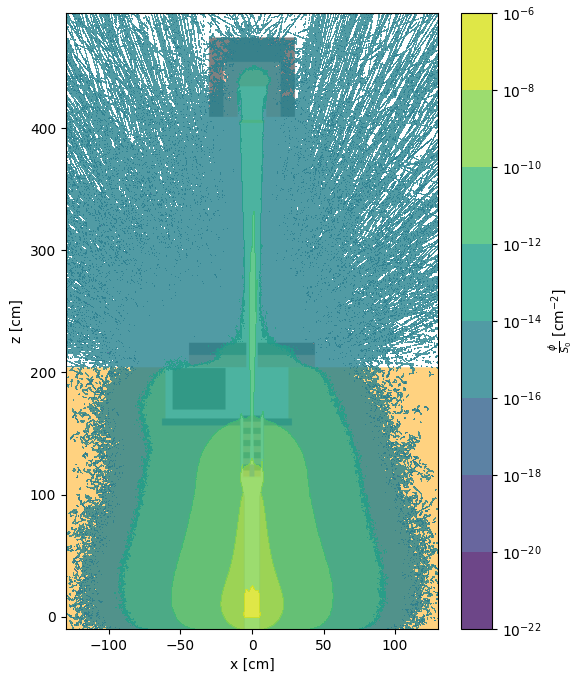
\includegraphics[width=0.7\textwidth]{conducto_flujo.png}
\caption{Distribución del flujo neutrónico en el modelo del conducto Nº5.}
\label{fig:conducto-flujo}
\end{figure}

Este comportamiento justifica la estrategia de desacoplar geométricamente la simulación del conducto respecto del núcleo del reactor. Simular directamente desde el núcleo implicaría combinar la baja probabilidad de que los neutrones alcancen la entrada del conducto con la también baja probabilidad de que atraviesen el colimador y lleguen al banco de detectores, resultando en una estadística reducida. En cambio, al utilizar la fuente distribucional en la entrada del conducto como fuente, se logra concentrar los recursos computacionales en la región de interés, obteniendo una estadística adecuada para el análisis espectral y mejorando los resultados.

\subsection{Comparación con la medición experimental}

La Figura~\ref{fig:conducto-espectro} muestra el espectro neutrónico obtenido en el banco de detectores a partir de la simulación con fuente distribucional, en comparación con el espectro medido experimentalmente mediante TdV. Se observa concordancia a partir de energías del orden de 0.01~eV. No obstante, por debajo de ese umbral, el flujo simulado subestima al medido experimentalmente.

\begin{figure}[h]
\centering
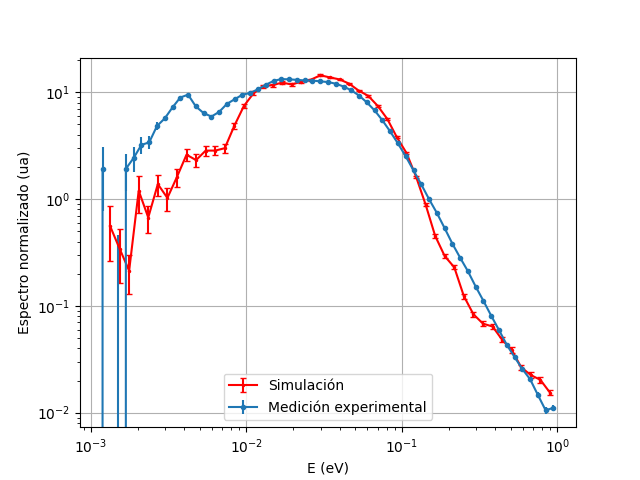
\includegraphics[width=\textwidth]{conducto_espectro.png}
\caption{Comparación del espectro de neutrones obtenido en el banco de detectores en la simulación de \texttt{OpenMC} con la medición experimental realizada por TdV por el Departamento de Neutrones del CAB.}
\label{fig:conducto-espectro}
\end{figure}

Esta discrepancia en la región de bajas energías puede atribuirse principalmente a dos factores:

\begin{itemize}
\item \textbf{Limitaciones en la representación espectral de la fuente}. Tal como se observa en la Figura~\ref{fig:conducto-comparacion-let}, existe diferencia entre el archivo original y la fuente distribucional en la región de mayor letargía, correspondiente a las energías menores a 0.01~eV. Esta desviación se origina en la discretización inherente al método de histogramas.
\item \textbf{Tratamiento del filtro de bismuto en la simulación}. En la modelización realizada con \texttt{OpenMC}, se emplean secciones eficaces correspondientes a átomos de bismuto como gas libre. Sin embargo, el filtro real está construido con bismuto cristalino, cuyas secciones eficaces difieren a bajas energías \cite{Mishra2006PULSTAR}. Mientras que para energías superiores a 0.1~eV ambas secciones eficaces son equivalentes, por debajo de ese valor la sección eficaz del bismuto cristalino es menor. La máxima discrepancia se presenta en torno a 1~meV, donde la sección eficaz del bismuto cristalino representa apenas el 10\% de la correspondiente al bismuto libre. Este efecto conduce a una atenuación del flujo térmico simulado, explicando la subestimación observada en la comparación con los datos experimentales.
\item \textbf{Tratamiento experimental de los datos medidos}. La medición experimental utilizada como referencia ha sido obtenida a partir de mediciones realizadas con detectores de ${}^3$He, y requiere un proceso de postratamiento. Este proceso incluye correcciones por tiempo muerto de los detectores, eficiencia de detección de los detectores de ${}^3$He y por nivel de fondo. En particular, la estimación y substracción del nivel de fondo puede introducir cierta variabilidad en la forma final del espectro, especialmente en la región correspondiente a menores energías. Como es esta la región del espectro donde se registra la mayor discrepancia respecto a la simulación, no puede descartarse que parte del desvío observado esté asociado a incertidumbres propias del procedimiento de corrección experimental aplicado.
\end{itemize}

A pesar de estas limitaciones, los resultados obtenidos permiten validar el enfoque implementado, demostrando que la fuente distribucional construida es capaz de reproducir adecuadamente el comportamiento espectral de los neutrones en el banco de detectores en el rango de interés térmico.


\chapter{Conclusiones}
\label{chap:conclusiones}

En este trabajo se desarrolló e implementó un método para generar fuentes distribucionales para simulaciones Monte Carlo basado en el uso de histogramas multidimensionales. La implementación se realizó dentro del código \texttt{KDSource}.

La metodología desarrollada fue validada mediante pruebas analíticas y contra mediciones experimentales, confirmando su capacidad para reproducir distribuciones en el espacio de fases. En particular, se mostró que la estructura de histogramas multidimensionales empleada logra preservar satisfactoriamente las correlaciones de las variables del espacio de fases de las partículas.

Adicionalmente, se implementó un esquema de bineado adaptativo, el cual permitió captar con precisión regiones donde las distribuciones exhiben cambios bruscos, deltas o bordes definidos, incrementando la resolución local del histograma de manera autónoma. Este esquema resultó especialmente útil en situaciones donde las distribuciones presentan estructuras complejas difíciles de caracterizar mediante discretizaciones uniformes.

Por otro lado, se realizó una implementación específica de remuestreo \textit{on-the-fly} dentro del código fuente de \texttt{OpenMC}. Esta modificación permitió el remuestreo de partículas durante la ejecución de la simulación, sin la necesidad de generar listas intermedias de partículas. La técnica se aplicó en el caso del conducto Nº5 del reactor RA-6, obteniendo resultados en concordancia con datos experimentales disponibles, validando así el método desarrollado.

\subsection*{Trabajo futuro}

A partir de los resultados obtenidos y las capacidades mostradas por el método implementado, se identifican diversas líneas futuras de investigación que podrían extender su alcance y utilidad práctica. Una primera línea consiste en la generalización del método hacia otras geometrías más complejas y variadas, más allá de las superficies planas consideradas en este trabajo. Esto incluiría, por ejemplo, fuentes distribuidas sobre superficies curvas o laterales de un conducto.

Adicionalmente, sería valioso incorporar técnicas que permitan un refinamiento local dirigido por el usuario. En particular, podría implementarse la capacidad de especificar manualmente un mayor número de bines en rangos específicos para ciertas variables, mejorando selectivamente la resolución de la distribución sin afectar la estructura general de macrogrupos utilizada. Esta capacidad permitiría a los usuarios optimizar el detalle local en la generación de fuentes, adaptándose de manera flexible a distintos escenarios y necesidades de simulación.

Finalmente, dado que el método desarrollado ha sido implementado únicamente para neutrones, sería relevante extender su aplicación a otras partículas, como fotones, ampliando así sus posibles aplicaciones en simulaciones Monte Carlo.


\appendix
% \appendix
\chapter{Implementación computacional del método de generación de fuentes Monte Carlo mediante histogramas multidimensionales}
\label{app:B}


En este apéndice se presenta la implementación computacional del método de generación de fuentes Monte Carlo mediante histogramas multidimensionales. Se detallan los principales componentes, abarcando tanto el procesamiento en \texttt{Python} y \texttt{C/C++} como la integración con \texttt{OpenMC}:

\begin{itemize}
    \item El procesamiento de un archivo \texttt{HDF5} en \texttt{Python}, incluyendo la construcción de la estructura \texttt{TreeNode} a partir de los datos de partículas.
    \item El algoritmo de \textit{bineado} adaptativo implementado en \texttt{Python} y un ejemplo de cómo se genera el archivo \texttt{XML} resultante.
    \item La implementación en \texttt{C/C++} de la clase \texttt{HistogramSource} dentro de \texttt{OpenMC}, con foco en la función \texttt{fill\_particle} y en la forma de utilizar esta fuente para una simulación.
\end{itemize}

\vspace{0.5em}
\noindent
El código fuente completo del proyecto se encuentra disponible en un repositorio público de \textit{GitHub} \cite{RepositorioKDSource2025} \cite{RepositorioOpenMCSource2025}.

\section{Procesamiento de un archivo \texttt{HDF5} en \texttt{Python}}\label{sec:procesamiento_h5}

Para extraer la información de un archivo \texttt{HDF5} generado por \texttt{OpenMC} y construir los histogramas multidimensionales, se emplea el módulo \texttt{histograms.py}. A continuación se describe el procedimiento principal:

\begin{enumerate}
    \item Lectura de variables del espacio de fases (energía, posición y ángulo) y pesos estadísticos.
    \item Construcción de un \texttt{DataFrame} de \texttt{pandas} que contenga:
    \[
      \{\texttt{ln(E0/E)},\, x,\, y,\, \mu,\, \phi,\, \texttt{wgt}\}.
    \]
    \item Ejecución recursiva de la función \texttt{build\_node}, que genera un árbol de nodos \texttt{TreeNode}.
\end{enumerate}

\subsection{Estructura \texttt{TreeNode}}\label{subsec:treenode}

Cada nodo del árbol jerárquico almacena la distribución acumulada (CDF), los bordes de micro-bines, los bordes de macro-bines y los punteros a sus hijos. La clase en \texttt{Python} se define de la siguiente forma:

\begin{minted}[fontsize=\footnotesize, linenos, frame=lines]{python}
class TreeNode:
    """Nodo elemental de un árbol jerárquico de histogramas multidimensionales.

    Cada nodo contiene:
    - **distribucion_acumulada** – Vector CDF (incluye un 0 inicial) para muestreo.
    - **bordes_micro** – Bordes del histograma fino (bins “micro”).
    - **bordes_macro** – Bordes del histograma grueso (bins “macro”).
    - **hijos** – Lista de subnodos.

    Atributos
    ----------
    distribucion_acumulada : Optional[np.ndarray]
        Vector de la distribución acumulada (CDF). None en hojas sin datos.
    bordes_micro : Optional[np.ndarray]
        Bordes de bins finos. None en hojas sin datos.
    bordes_macro : Optional[np.ndarray]
        Bordes de bins gruesos para particionar en hijos. 
        None si es última dimensión.
    hijos : List[TreeNode]
        Lista de nodos hijos (subárboles) en orden de bins_macro.
    """

    # ---------------------------------------------------------------------
    # Constructor: convertimos a `np.ndarray` sólo si los vectores existen.
    # ---------------------------------------------------------------------
    def __init__(
        self,
        distribucion_acumulada: Optional[Sequence[float]],
        bordes_micro: Optional[Sequence[float]],
        bordes_macro: Optional[Sequence[float]],
    ) -> None:
        # Inicializamos lista de hijos vacía
        self.hijos: List[TreeNode] = []

        # Convertimos secuencias a np.ndarray si existen, manteniendo dtype float
        if distribucion_acumulada is not None:
            self.distribucion_acumulada: np.ndarray = np.asarray(
                distribucion_acumulada, dtype=float
            )
        else:
            self.distribucion_acumulada = None

        if bordes_micro is not None:
            self.bordes_micro: np.ndarray = np.asarray(
                bordes_micro, dtype=float
            )
        else:
            self.bordes_micro = None

        if bordes_macro is not None:
            self.bordes_macro: np.ndarray = np.asarray(
                bordes_macro, dtype=float
            )
        else:
            self.bordes_macro = None

    def add_child(self, hijo: "TreeNode") -> None:
        """Añade un nodo hijo al final de la lista de hijos.

        Args:
            hijo (TreeNode): Nodo que se desea incorporar como subárbol.
        """
        self.hijos.append(hijo)

    def to_xml(self) -> ET.Element:
        """Serializa el nodo (y recursivamente sus hijos) a un elemento XML.

        Cada nodo se representa como:
        <node>
          <cumul>...valores separados por comas o "None"</cumul>
          <micro>...bordes_micro separados por comas o "None"</micro>
          <macro>...bordes_macro separados por comas o "None"</macro>
          <!-- subnodos aquí -->
        </node>

        Returns:
            ET.Element: Elemento <node> con sus etiquetas internas y subnodos.
        """
        nodo_elem = ET.Element("node")

        # Convertimos cada vector a texto CSV; si es None, escribimos "None"
        etiquetas = ("cumul", "micro", "macro")
        vectores = (
            self.distribucion_acumulada,
            self.bordes_micro,
            self.bordes_macro,
        )

        for etiqueta, vector in zip(etiquetas, vectores):
            subelem = ET.SubElement(nodo_elem, etiqueta)
            if vector is None:
                subelem.text = "None"
            else:
                # .tolist() asegura que sea iterable de Python puro
                subelem.text = ",".join(map(str, vector.tolist()))

        # Añadimos los hijos de forma recursiva
        for hijo in self.hijos:
            nodo_elem.append(hijo.to_xml())

        return nodo_elem
\end{minted}

\noindent En esta estructura:
\begin{itemize}
    \item \texttt{distribucion\_acumulada} contiene la función de distribución acumulada (CDF) normalizada, incluyendo un cero inicial. Su longitud es igual al número de micro-bines más uno.
    \item \texttt{bordes\_micro} define los bordes del histograma fino (micro-bines), utilizados para el muestreo de la variable en el nodo actual.
    \item \texttt{bordes\_macro} define los bordes del histograma grueso (macro-bines), que particionan el dominio y determinan los subnodos (hijos).
    \item \texttt{hijos} es la lista de subnodos jerárquicos, con una cantidad dada por
    \[
        \lvert \texttt{hijos} \rvert \;=\; \lvert \texttt{bordes\_macro} \rvert - 1,
    \]
    ya que cada intervalo definido por \texttt{bordes\_macro} representa una rama independiente del árbol.
\end{itemize}

\noindent La clase incluye tres métodos principales:
\begin{itemize}
    \item \texttt{\_\_init\_\_}: inicializa un nodo, convirtiendo los vectores de entrada en arreglos de tipo \texttt{numpy} si están definidos, y creando una lista vacía de hijos.
    \item \texttt{add\_child}: incorpora dinámicamente un subnodo al árbol, agregándolo al final de la lista \texttt{hijos}.
    \item \texttt{to\_xml}: serializa el nodo actual y sus hijos a un elemento XML, escribiendo los vectores como cadenas separadas por comas y anidando recursivamente los subnodos. Este método permite almacenar la estructura completa del árbol jerárquico en un único archivo \texttt{XML}.
\end{itemize}

\subsection{Construcción recursiva del árbol}\label{subsec:build_node}

La función principal que construye este árbol se denomina \texttt{build\_node}. Esta función recibe el \texttt{DataFrame} con la información del archivo de partículas y la configuración de procesamiento. Su código es:

\begin{minted}[fontsize=\footnotesize, linenos, frame=lines]{python}
def build_node(
    df: pd.DataFrame,
    columns: Sequence[str],
    micro_bins: Sequence[int],
    macro_bins: Sequence[int],
    micro_initial_bins: Sequence[Optional[int]],
    macro_initial_bins: Sequence[Optional[int]],
    micro_binning: str,
    macro_binning: str,
    user_edges: Sequence[Optional[List[float]]],
) -> TreeNode:
    """
    Construye recursivamente un TreeNode a partir de un DataFrame, discretizando
    sucesivamente según la lista de `columns` en dimensiones jerárquicas.

    Cada nivel crea:
        - macro_edges: bordes de macro-bins (si hay más dimensiones por procesar),
        - micro_edges + cumul: bordes de micro-bins y su CDF correspondiente.

    Parámetros
    ----------
    df : pd.DataFrame
        Subconjunto de tracks (cada fila es un evento), que debe contener:
            - Columnas numéricas en `columns`.
            - Columna "wgt" con pesos para cada fila.
    columns : Sequence[str]
        Lista de nombres de columnas que se discretizarán en orden jerárquico.
    micro_bins : Sequence[int]
        Número de micro-bins a generar para cada dimensión (paralelo a `columns`).
    macro_bins : Sequence[int]
        Número de macro-bins a generar para cada dimensión (paralelo a `columns`).
    micro_initial_bins : Sequence[Optional[int]]
        Parámetros initial_bins para binning adaptativo en micro-bins por dimensión.
        Debe tener la misma longitud que `columns`.
    macro_initial_bins : Sequence[Optional[int]]
        Parámetros initial_bins para binning adaptativo en macro-bins por dimensión.
        Debe tener la misma longitud que `columns`.
    micro_binning : str
        Estrategia de micro-binning: 'equal_bins' o 'adaptive'.
    macro_binning : str
        Estrategia de macro-binning: 'equal_bins' o 'adaptive'.
    user_edges : Sequence[Optional[List[float]]]
        Lista de listas de bordes de usuario para cada dimensión.
        Cada elemento puede ser None (no hay bordes forzados) o una lista de floats.

    Retorna
    -------
    TreeNode
        Nodo raíz que contiene:
            - cumul: CDF de la primera dimensión (o None si no aplica).
            - micro_edges: bordes de micro-bins en la primera dimensión.
            - macro_edges: bordes de macro-bins en la primera dimensión.
        Y sus hijos correspondientes para las siguientes dimensiones.
    """
    # -------------------------------------------------------------------------
    # 1. Caso base: si no hay eventos, devolvemos un nodo “vacío” sin bordes.
    # -------------------------------------------------------------------------
    if df.empty:
        # TreeNode acepta (cumul, micro_edges, macro_edges). 
        # Pasamos None para indicar vacío.
        return TreeNode(None, None, None)

    # Nombre de la columna actual sobre la que estamos trabajando
    col = columns[0]

    # -------------------------------------------------------------------------
    # 2. Manejo de la “especialidad”: todos los eventos en esta dimensión 
    # son idénticos
    # -------------------------------------------------------------------------
    # Si todos los valores en df[col] son iguales, no tiene sentido calcular 
    # múltiples bines.
    # Definimos micro_edges triviales y, si hay más dimensiones, generamos 
    # macro_edges minimal.
    if df[col].min() == df[col].max():
        valor_constante = float(df[col].min())

        # Si es la última dimensión, no necesitamos macro_edges
        if len(columns) == 1:
            macro_edges: Optional[np.ndarray] = None
        else:
            # Para asegurar que haya al menos dos extremos y no crashear 
            # np.digitize, generamos un rango [valor-1, valor+1] (o cualquier 
            # delta pequeño).
            macro_edges = np.array(
                [valor_constante - 1.0, valor_constante + 1.0]
            )

        # micro_edges queda en un único punto (el valor constante)
        micro_edges = np.array([valor_constante], dtype=float)
        # La CDF acumulada es trivial: toda la probabilidad en ese único punto
        cumul = np.array([1.0], dtype=float)

    else:
        # ---------------------------------------------------------------------
        # 3. Cálculo de macro_edges (si corresponde) en esta dimensión
        # ---------------------------------------------------------------------
        if len(columns) == 1:
            # Última dimensión: no necesitamos macro_edges
            macro_edges = None
        else:
            # Llamamos a la función refactorizada `determine_macro_edges`
            macro_edges = determine_macro_edges(
                df,
                col,
                macro_bins[0],
                macro_binning,
                user_edges[0],
                initial_bins=macro_initial_bins[0],
            )
            if macro_edges is None:
                print("macro_edges is None")

        # ---------------------------------------------------------------------
        # 4. Cálculo de micro_edges y su CDF (cumul) en esta dimensión
        # ---------------------------------------------------------------------
        micro_edges, cumul = compute_micro_edges_and_cumul(
            df,
            col,
            micro_bins[0],
            micro_binning,
            macro_edges,
            initial_bins=micro_initial_bins[0],
        )

    # Creamos el nodo actual con los resultados en esta dimensión
    node = TreeNode(cumul, micro_edges, macro_edges)

    # -------------------------------------------------------------------------
    # 5. Caso recursivo: si hay más columnas, creamos hijos para cada macro-bin
    # -------------------------------------------------------------------------
    if len(columns) > 1:
        # Si no hay macro_edges (por ser última dimensión), no hay recursión
        if macro_edges is None:
            return node

        # 5.1 Calculamos el índice de macro-bin para cada fila en df
        # np.digitize devuelve índices de bin (1-based) para cada valor en df[col].
        # Restamos 1 para pasar a 0-based.
        idx = np.digitize(df[col].to_numpy(), bins=macro_edges) - 1

        total_macro_bins = (
            len(macro_edges) - 1
        )  # Cantidad de intervalos macrobins

        for i in range(total_macro_bins):
            # -----------------------------------------------------------------
            # 5.2 Construcción de la máscara para extraer sub-DataFrame en el bin i
            # -----------------------------------------------------------------
            # Truco de KDSource: en el penúltimo bin (i == total_macro_bins - 2),
            # incluimos también los que quedaron en el último bin (i+1)
            # para abarcar el rango abierto derecho.
            # if total_macro_bins > 1 and i == total_macro_bins - 2:
            #     mask = (idx == i) | (idx == i + 1)
            # else:
            #     mask = idx == i

            mask = (
                (idx == i) | ((i == len(macro_edges) - 2) & (idx == i + 1))
                if len(macro_edges) > 2
                else (idx == i)
            )

            # df filtrado de eventos cuya coordenada col cae en el macro-bin i
            child_df = df[mask]

            # -----------------------------------------------------------------
            # 5.3 Llamada recursiva: descartamos la primera columna y avanzamos
            # -----------------------------------------------------------------
            child_node = build_node(
                child_df,
                columns[1:],  # Quitamos la primera dimension
                micro_bins[1:],  # Micro-bins de las dimensiones restantes
                macro_bins[1:],  # Macro-bins de las dimensiones restantes
                micro_initial_bins[
                    1:
                ],  # Parámetros initial_bins para micro-bins
                macro_initial_bins[
                    1:
                ],  # Parámetros initial_bins para macro-bins
                micro_binning,  # Misma estrategia para todas las dimensiones
                macro_binning,  # Misma estrategia para todas las dimensiones
                user_edges[1:],  # Bordes de usuario para dimensiones restantes
            )
            # Agregamos el nodo hijo a la lista de hijos del nodo actual
            node.add_child(child_node)

    return node
\end{minted}

\noindent La función \texttt{build\_node} implementa el método desarrolado en el trabajo. Su objetivo es generar un árbol de tipo \texttt{TreeNode} a partir de un conjunto de partículas representado como un \texttt{DataFrame}. La estructura resultante representa de forma recursiva la distribución multidimensional de las variables.

Cada nodo del árbol corresponde a una variable del espacio de fases, siguiendo el orden dado en \texttt{columns}. En cada nivel, el conjunto de eventos se divide primero mediante un histograma grueso (\texttt{macro\_bins}), generando subregiones que determinan los nodos hijos. Luego, dentro de cada subregión, se estima la distribución acumulada (CDF) sobre una grilla de histogramas finos (\texttt{micro\_bins}).

En particular:
\begin{itemize}
    \item Si todos los eventos presentan el mismo valor en una dimensión, se utiliza una discretización trivial y se evita la creación innecesaria de bins.
    \item Si no hay más dimensiones por procesar, el nodo creado se considera una hoja del árbol.
    \item Si existen más dimensiones, se invoca recursivamente \texttt{build\_node} sobre cada subconjunto definido por los macro-bines, construyendo los hijos correspondientes.
\end{itemize}

Esta estructura es la que luego se serializa en formato \texttt{XML} mediante el método \texttt{to\_xml} para el muestreo de partículas en etapas posteriores.

\section{\textit{Bineado} adaptativo y generación del \texttt{XML}}\label{sec:bineado_adaptativo}

En esta sección se detalla el algoritmo de \textit{bineado} adaptativo utilizado tanto para los macro-bines como para los micro-bines. Se ejemplifica a continuación la función para obtener bordes adaptativos en una sola dimensión:

\subsection{Función de \textit{bineado} adaptativo en \texttt{Python}}

\begin{minted}[fontsize=\footnotesize, linenos, frame=lines]{python}
    def obtener_bordes_adaptativos(
        datos: np.ndarray,
        num_bins: int,
        pesos: Optional[np.ndarray] = None,
        *,
        initial_bins: int = 6,
        fine_bins: int = 50_000,
        user_edges: Optional[Sequence[float]] = None,
    ) -> np.ndarray:
        """
        Calcula bordes adaptativos para un histograma de `num_bins` usando el 
        criterio |ΔCDF|máx.
    
        El procedimiento realiza los siguientes pasos:
          1. Construye un arreglo inicial de `initial_bins + 1` bordes 
          equiespaciados entre el mínimo y máximo de `datos`.
          2. Inserta, si se proporcionan, los `user_edges` dentro del rango 
          [mín, max], descartando los que queden fuera y eliminando duplicados.
          3. Calcula una CDF de alta resolución (`fine_bins + 1` bordes) para tener
             una referencia "casi continua" de la distribución de los datos.
          4. Repite `extra_bordes = num_bins - initial_bins` veces:
             a. Calcula la CDF actual usando los bordes gruesos.
             b. Interpola la CDF gruesa en los puntos finos.
             c. Encuentra el índice donde la diferencia absoluta
             |CDF_fina - CDF_gruesa_interp| es máxima.
             d. Inserta ese punto (de la división fina) como nuevo borde en el 
             arreglo grueso.
          5. Devuelve los `num_bins + 1` bordes finales, ordenados de menor a mayor.
    
        Parámetros
        ----------
        datos : np.ndarray
            Vector unidimensional de datos de entrada.
        num_bins : int
            Número total de bines deseados (cantidad de intervalos = num_bins,
            cantidad de bordes = num_bins + 1).
        pesos : Optional[np.ndarray]
            Arreglo de pesos asociado a cada dato (misma longitud que `datos`).
            Si es None, se asume peso uniforme = 1 para cada punto.
        initial_bins : int, opcional (por defecto = 6)
            Número inicial de bines gruesos (antes de refinar).
            Debe cumplir 1 ≤ initial_bins < num_bins.
        fine_bins : int, opcional (por defecto = 50000)
            Resolución de la malla fina usada para estimar la CDF de referencia.
            Entre más grande, más precisa la ubicación de los bordes óptimos, pero
            aumenta el costo computacional.
        user_edges : Optional[Sequence[float]], opcional
            Lista de bordes que el usuario quiere insertar obligatoriamente. Estos
            se agregan sólo si están dentro del rango [mín(datos), máx(datos)].
    
        Retorna
        -------
        np.ndarray
            Vector ordenado de longitud `num_bins + 1` con los bordes adaptativos
            que garantizan minimizar el error máximo de la CDF en cada paso.
        """
        if num_bins <= initial_bins:
            raise ValueError(
                "El número de bines deseados 'num_bins' debe ser mayor que
                 'initial_bins'."
            )
    
        # 1. Determinamos los extremos de los datos
        minimo = float(np.min(datos))
        maximo = float(np.max(datos))
    
        # 2. Construimos bordes equiespaciados iniciales (initial_bins + 1)
        bordes = np.linspace(minimo, maximo, initial_bins + 1)
    
        # 3. Insertamos bordes de usuario si corresponden al rango y eliminamos 
        # duplicados
        if user_edges is not None:
            # Filtrar sólo los user_edges dentro de [mínimo, maximo]
            bordes_usuario_filtrados = [
                b for b in user_edges if minimo <= b <= maximo
            ]
            if bordes_usuario_filtrados:
                # Concatenamos, unificamos y ordenamos
                bordes = np.sort(
                    np.unique(np.concatenate((bordes, bordes_usuario_filtrados)))
                )
    
        # 4. Calculamos CDF de alta resolución para referencia
        bordes_finos = np.linspace(minimo, maximo, fine_bins + 1)
        _, cdf_fina = calcular_cdf_ponderada(datos, bordes_finos, pesos)
    
        # 5. Insertamos iterativamente los bordes que maximizan |ΔCDF|
        extra_bordes = num_bins - initial_bins
        for _ in range(extra_bordes):
            # 5.a. CDF en bordes gruesos actuales
            _, cdf_gruesa = calcular_cdf_ponderada(datos, bordes, pesos)
    
            # 5.b. Interpolamos la CDF gruesa en los puntos finos
            #     Usamos np.interp: interpola cdf_gruesa(bordes) en coordenadas 
            # bordes_finos
            cdf_gruesa_interp = np.interp(bordes_finos, bordes, cdf_gruesa)
    
            # 5.c. Calculamos la diferencia absoluta con la CDF fina y buscamos el 
            # máximo
            diferencias = np.abs(cdf_fina - cdf_gruesa_interp)
            indice_max = int(np.argmax(diferencias))
    
            # 5.d. Insertamos el borde fino correspondiente y reordenamos
            nuevo_borde = bordes_finos[indice_max]
            bordes = np.sort(np.append(bordes, nuevo_borde))
    
        return bordes
\end{minted}

\noindent Donde la función auxiliar \texttt{calcular\_cdf\_ponderada} es:

\begin{minted}[fontsize=\footnotesize, linenos, frame=lines]{python}
    def calcular_cdf_ponderada(
        datos: np.ndarray, bordes: np.ndarray, pesos: Optional[np.ndarray] = None
    ) -> Tuple[np.ndarray, np.ndarray]:
        """
        Calcula la función de distribución acumulada (CDF) ponderada en puntos dados.
    
        Esta función construye un histograma de `datos` utilizando los `bordes`
        especificados y, opcionalmente, aplica un arreglo de `pesos` a cada dato.
        A partir de las frecuencias, se obtiene la CDF normalizada (entre 0 y 1).
    
        Parámetros
        ----------
        datos : np.ndarray
            Vector unidimensional de datos a discretizar.
        bordes : np.ndarray
            Arreglo de longitud N+1 que define los bordes de los bines donde se 
            evaluará la CDF.
        pesos : Optional[np.ndarray]
            Arreglo de pesos, de la misma longitud que `datos`. Si es None, se 
            asume peso=1 para cada dato.
    
        Retorna
        -------
        Tuple[np.ndarray, np.ndarray]
            - bordes : np.ndarray
                Copia de los bordes de entrada (sin modificar).
            - cdf : np.ndarray
                Vector de longitud N+1 con los valores de la CDF normalizada 
                evaluada en cada borde.
                Notar que se inserta un 0 al inicio para representar la CDF antes 
                del primer bin.
        """
        # Obtenemos los conteos ponderados por bin
        conteos, _ = np.histogram(datos, bins=bordes, weights=pesos)
    
        # Construimos la CDF acumulada y agregamos un 0 inicial para la 
        # interpolación
        cdf = np.insert(np.cumsum(conteos), 0, 0.0)
    
        # Normalizamos la CDF en [0,1], evitando división por cero si todos los 
        # conteos son cero
        total = cdf[-1]
        if total:
            cdf = cdf / total
    
        return bordes.copy(), cdf
\end{minted}

\subsection{Ejemplo de archivo \texttt{XML} generado}\label{subsec:xml_generado}

Una vez construido el árbol completo (\texttt{TreeNode}), se genera el archivo \texttt{XML} que define la fuente para \texttt{OpenMC}. El formato general del archivo \texttt{source.xml} es el siguiente:

\begin{minted}[fontsize=\footnotesize, linenos, frame=lines, bgcolor=LightGray]{xml}
<HistogramSource>
  <J> <!-- Corriente escalar -->
    1.2345e-3
  </J>
  <ParticleType> neutron </ParticleType>
  <z> 15.0 </z>
  <VariableOrder> ln(E0/E),x,y,mu,phi </VariableOrder>
  <SurfaceGeometry> rectangular </SurfaceGeometry>
  <!-- Si SurfaceGeometry == circular, incluir <Radius> R </Radius> -->
  <!-- A continuación, se anidan los nodos <node> del árbol de histogramas -->
  <node>
    <cumul>0.000,0.200,0.450,0.700,0.900,1.000</cumul>
    <micro> ... valores separados por comas ... </micro>
    <macro> ... valores separados por comas ... </macro>
    <!-- Subnodos -->
    <node>
        <cumul> ... </cumul>
        <micro> ... </micro>
        <macro> ... </macro>
        <!-- Y así sucesivamente -->
    </node>
    <node> ... </node>
    <!-- ... -->
  </node>
</HistogramSource>
\end{minted}

\noindent En este XML:
\begin{itemize}
    \item \texttt{<J>} contiene la corriente escalar \(J = \sum w_i / N\).
    \item \texttt{<ParticleType>} indica ``neutron'' o ``photon''.
    \item \texttt{<z>} es la coordenada de la superficie de registro (en cm).
    \item \texttt{<VariableOrder>} es la lista CSV de variables procesadas, por ejemplo \texttt{ln(E0/E),x,y,mu,phi}.
    \item \texttt{<SurfaceGeometry>} es ``rectangular'' o ``circular''. En el caso circular, se incluye \texttt{<Radius>R</Radius>} debido a que esta opcion permite verificar que las particulas generadas aparecen dentro de un radio R dado. En caso de que aparezcan fuera de este radio se vuelve a sortear la posicion hasta que aparecen dentro del radio.
    \item Cada etiqueta \texttt{<node>} contiene:
    \begin{itemize}
        \item \texttt{<cumul>}: valores de la CDF en los bordes de micro-nivel.
        \item \texttt{<micro>}: bordes de micro-bines separados por comas.
        \item \texttt{<macro>}: bordes de macro-bines separados por comas.
        \item Subnodos anidados para las dimensiones siguientes.
    \end{itemize}
\end{itemize}

De este modo, el archivo \texttt{XML} contiene toda la parametrización jerárquica que describe la fuente.

\section{Implementación  de \texttt{HistogramSource} en \texttt{C/C++} para \texttt{OpenMC}}\label{sec:histogramsource_c}

Para integrar la fuente jerárquica en \texttt{OpenMC}, se definió la clase \texttt{HistogramSource} en \texttt{C++}. A continuación se muestran los fragmentos más relevantes.

\subsection{Definición de \texttt{HistogramSource} en \texttt{source.h}}\label{subsec:source_h}

\begin{minted}[fontsize=\footnotesize, linenos, frame=lines, bgcolor=LightGray]{cpp}
    /*! \class HistogramSource
     *  \brief Fuente compuesta a partir de histogramas cargados desde XML.
     */
    class HistogramSource : public Source {
    public:
      explicit HistogramSource(pugi::xml_node node);
      ~HistogramSource() override;
    
      // Muestrea un punto del espacio de fases usando el árbol de histogramas
      SourceSite sample(uint64_t* seed) const override;
    
    private:
      TreeNode* cumul_micro_macro;  // Raíz del árbol (definido en histograms.h)
      HSHeader* header;             // Estructura con J, z0, var_order, etc.
      double z0;                    // Coordenada z de la superficie
      ParticleType particle;        // Tipo de partícula ("neutron" o "photon")
      std::vector<std::string> variable_order; // Orden de variables
      std::string surface_geometry; 
      double surface_radius;        // Si circular
    };
    \end{minted}
    

\noindent El constructor lee el XML y construye el árbol:

\begin{minted}[fontsize=\footnotesize, linenos, frame=lines, bgcolor=LightGray]{cpp}
    HistogramSource::HistogramSource(pugi::xml_node node)
    {
      // 1. Obtener el path al archivo XML
      std::string path = get_node_value(node, "HistogramSource", false, true);
    
      // 2. Parsear el archivo XML
      pugi::xml_document doc;
      pugi::xml_parse_result result = doc.load_file(path.c_str());
      if (!result) {
        throw std::runtime_error("Error al cargar XML de HistogramSource: " +
                                 std::string(result.description()));
      }
    
      pugi::xml_node root = doc.child("HistogramSource");
    
      // 3. Leer la corriente J
      pugi::xml_node j_node = root.child("J");
      if (j_node) {
        strength_ = std::stod(j_node.child_value());
      } else {
        throw std::runtime_error("El nodo <J> no está presente en el archivo XML.");
      }
    
      // 4. Leer el tipo de partícula
      std::string particle_name = root.child("ParticleType").child_value();
      particle = string_to_particle(particle_name);
    
      // 5. Leer z0
      z0 = std::stod(root.child("z").child_value());
    
      // 6. Leer orden de variables
      std::string order_string = root.child("VariableOrder").child_value();
      variable_order = split_string(order_string);
    
      // 7. Leer geometría de la superficie
      surface_geometry = root.child("SurfaceGeometry").child_value();
    
      // 8. Leer radio de la superficie
      if (surface_geometry == "circular") {
        surface_radius = std::stod(root.child("Radius").child_value());
      }
    
      // 9. Construir el árbol recursivamente desde el nodo <node>
      pugi::xml_node root_node = root.child("node");
      if (!root_node) {
        throw std::runtime_error(
          "No se encontró el nodo raíz <node> del árbol jerárquico.");
      }
      cumul_micro_macro = parse_node(root_node);
    
      // 10. LLeno el header
      HSHeader* header_aux = (HSHeader*)malloc(sizeof(HSHeader));
      if (!header_aux) {
        fprintf(stderr, "Error: No se pudo asignar memoria para header.\n");
        exit(EXIT_FAILURE);
      }
      header_aux->J = strength_;
      if (particle == ParticleType::neutron) {
        header_aux->ptype = strdup("neutron");
      }
      header_aux->z = z0;
      header_aux->nvars = variable_order.size();
      header_aux->var_order = (char**)malloc(header_aux->nvars * sizeof(char*));
      for (int i = 0; i < header_aux->nvars; ++i) {
        header_aux->var_order[i] = (char*)malloc(variable_order[i].size() + 1);
        std::strcpy(header_aux->var_order[i], variable_order[i].c_str());
      }
    
      if (surface_geometry == "circular") {
        header_aux->surface_geometry = strdup("circular");
        header_aux->R = surface_radius;
      } else if (surface_geometry == "rectangular") {
        header_aux->surface_geometry = strdup("rectangular");
      } else {
        fprintf(stderr, "Error: Geometría de superficie no válida.\n");
        exit(EXIT_FAILURE);
      }
    
      header = header_aux;
    }
\end{minted}
   
\noindent
Este constructor de la clase \texttt{HistogramSource} se encarga de inicializar completamente la fuente a partir de un archivo \texttt{XML}. En primer lugar, extrae parámetros como la corriente escalar \(J\), el tipo de partícula, la posición de la superficie \(z_0\), el orden de las variables del espacio de fases y la geometría de la superficie. Posteriormente, llama a una función recursiva que interpreta el árbol de nodos \texttt{<node>} desde el XML y lo transforma en una estructura de tipo \texttt{TreeNode}, que permite muestrear partículas conforme a la distribución multidimensional almacenada.

Finalmente, se completa la estructura auxiliar \texttt{HSHeader}, que contiene la información relevante para ser utilizada por el código en tiempo de ejecución, como ser el orden de variables, el tipo de superficie y, si corresponde, su radio. Esta estructura facilita el acceso a los metadatos durante el muestreo sin necesidad de volver a consultar el archivo XML.
    

\subsection{Función \texttt{fill\_particle} y \texttt{traverse} (\texttt{histograms.c})}\label{subsec:fill_particle}

La función encargada de recorrer el árbol y rellenar la estructura \texttt{mcpl\_particle\_t} es \texttt{fill\_particle}. El proceso es:

\begin{enumerate}
  \item Generar, para cada nivel del árbol, un número aleatorio uniforme en \([0,1)\).
  \item Interpolar linealmente sobre la CDF (\texttt{cumul}) para obtener un valor continuo.
  \item Determinar el índice del macro-bin con \texttt{find\_interval} y avanzar al nodo hijo.
  \item Repetir hasta la última dimensión y asignar los valores a \texttt{mcpl\_particle\_t}.
\end{enumerate}

A continuación se muestra el código de \texttt{traverse} y \texttt{fill\_particle}:

\begin{minted}[fontsize=\footnotesize, linenos, frame=lines, bgcolor=LightGray]{c}
/**
 * Genera una partícula muestreada recursivamente a partir del árbol de histogramas.
 *
 * Esta función recorre el árbol de histogramas (estructura TreeNode) desde el nodo
 * raíz hasta una hoja, extrayendo en cada nivel un valor muestreado según la 
 * distribución almacenada.
 * El arreglo `valores_particula` debe tener la longitud adecuada (igual a la 
 * profundidad del árbol) y ya debe estar reservado por la función que invoca a 
 * `recorrer_arbol`.
 *
 * En cada nivel:
 * 1. Se genera un número aleatorio uniforme en [0,1).
 * 2. Se interpola linealmente este número sobre la CDF (`nodo_actual->cumul`)
 *    para obtener un valor continuo `valor_muestreado` en la escala “micro”
 *    (`nodo_actual->micro`).
 * 3. Se determina a qué “macro-grupo” pertenece `valor_muestreado` mediante
 *    la función `find_interval(valor_muestreado, nodo_actual->macro, 
 * nodo_actual->num_macro)`.
 * 4. Se avanza al hijo correspondiente (subnodo) y se almacena `valor_muestreado`
 *    en la posición `índice_nivel` del arreglo `valores_particula`.
 *
 * Cuando se llega a un nodo hoja (num_children == 0), se realiza un último muestreo
 * en ese nodo y se guarda el valor en la última posición de `valores_particula`.
 *
 * @param[in]  nodo_raíz           Puntero al nodo raíz del árbol (tipo TreeNode*).
 * @param[out] valores_particula   Arreglo de tipo double[] donde se almacenan los 
 *                                 valores muestreados.     
 *                                 Debe tener prealojada la memoria con tamaño 
 *                                 igual a la profundidad del árbol.
 *
 * @nota El árbol `TreeNode` debe cumplir que en cada nodo intermedio:
 *       - `micro` y `cumul` sean arreglos de igual longitud `num_micro > 0`.
 *       - `macro` sea un arreglo ordenado.
 *       - `children` sea un arreglo de punteros a `TreeNode` con 
 *       `num_children == num_macro - 1`.
 *
 * @nota Si en algún nivel `find_interval` retorna -1 (valor fuera de rango),
 *       se imprimirá un mensaje de error en stderr y la función continuará con la 
 *       siguiente iteración.
 *       Se asume que las distribuciones están correctamente definidas y 
 *       normalizadas en [0,1].
 */
 void traverse(TreeNode *nodo_raíz, double valores_particula[])
 {
     // Índice para recorrer el arreglo de salida
     int indice_nivel = 0;
 
     // Nodo actual inicia en la raíz
     TreeNode *nodo_actual = nodo_raíz;
 
     // Iterar mientras haya hijos (nodo no sea hoja)
     while (nodo_actual->num_children > 0)
     {
         // 1. Generar número aleatorio uniforme en [0,1)
         double aleatorio = (double)rand() / RAND_MAX;
 
         // 2. Interpolar linealmente sobre la CDF (cumul) usando el arreglo de 
         //    micro-bins para obtener el valor continuo en “micro”.
         double valor_muestreado = interpolacion_lineal(
             aleatorio,
             nodo_actual->micro,
             nodo_actual->cumul,
             nodo_actual->num_micro);
 
         // 3. Encontrar el índice de la macro-banda donde cae el valor muestreado
         int idx_macro = find_interval(
             valor_muestreado,
             nodo_actual->macro,
             nodo_actual->num_macro);
 
         if (idx_macro < 0)
         {
             // Si el valor muestreado está fuera de rango de las bandas “macro”
             fprintf(stderr,
                     "Error: valor muestreado %.6f fuera de rangos macro",
                     valor_muestreado,
                     indice_nivel);
             // Se continúa para intentar en el siguiente nivel (aunque lógicamente
             // este caso no debería ocurrir si las distribuciones están bien 
             // definidas).
         }
         else
         {
             // 4. Avanzar al hijo correspondiente y guardar el valor en el arreglo 
             // de la partícula
             nodo_actual = nodo_actual->children[idx_macro];
         }
 
         valores_particula[indice_nivel] = valor_muestreado;
         indice_nivel++;
     }
 
     // Al llegar a un nodo hoja, realizar un último muestreo en ese nodo
     double aleatorio_final = (double)rand() / RAND_MAX;
     double valor_final = interpolacion_lineal(
         aleatorio_final,
         nodo_actual->micro,
         nodo_actual->cumul,
         nodo_actual->num_micro);
     valores_particula[indice_nivel] = valor_final;
 }
\end{minted}

\begin{minted}[fontsize=\footnotesize, linenos, frame=lines, bgcolor=LightGray]{c}
/**
 * Rellena un mcpl_particle_t con valores muestreados del árbol de histogramas.
 *
 * Esta función genera una partícula a partir de un árbol jerárquico de histogramas 
 * (TreeNode) y del encabezado HSHeader, que define parámetros como la geometría de
 * la superficie ("rectangular" o "circular"), el radio R (si corresponde) y la 
 * coordenada z de la fuente.
 * El muestreo se realiza nivel por nivel: en cada nivel se extrae un valor de la
 * distribución acumulada (CDF) mediante interpolación lineal. En el caso de 
 * geometría circular, se impone la restricción x² + y² ≤ R² al muestrear los dos 
 * primeros grados de libertad espaciales.
 *
 * @param[out] particula_mcpl     Puntero al struct mcpl_particle_t que se va a 
 *                                rellenar.
 * @param[in]  arbol_histograma   Puntero al nodo raíz del árbol de histogramas 
 *                                (TreeNode).
 * @param[in]  encabezado_hs      Puntero a HSHeader con parámetros de la fuente:
 *                                - nvars: número de variables a muestrear en cada 
 *                                partícula.
 *                                - surface_geometry: "rectangular" o "circular".
 *                                - R: radio máximo permitido (solo si 
 *                                surface_geometry == "circular").
 *                                - z: coordenada z fija de la superficie fuente.
 *
 * Notar:
 * - Se reserva dinámicamente un arreglo intermedio de tamaño encabezado_hs->nvars
 *   para almacenar los valores muestreados en cada nivel del árbol. Al final de la
 *   función, este arreglo se libera.
 * - Si ocurre cualquier error (memoria, geometría no soportada, o no poder 
 *   muestrear dentro del círculo tras varios intentos), la función termina el 
 *   programa con exit(EXIT_FAILURE).
 */
 void fill_particle(mcpl_particle_t *particula_mcpl, TreeNode *arbol_histograma,
  HSHeader *encabezado_hs)
 {
     // Verificar parámetros obligatorios
     if (particula_mcpl == NULL || arbol_histograma == NULL || encabezado_hs == NULL)
     {
         fprintf(stderr, "Error en fill_particle: puntero nulo.\n");
         exit(EXIT_FAILURE);
     }
 
     // Reservar espacio para almacenar los valores muestreados de la partícula
     double *valores_particula = (double *)malloc(encabezado_hs->nvars * sizeof(double));
     if (valores_particula == NULL)
     {
         fprintf(stderr, "Error en fill_particle: no se pudo asignar memoria.\n");
         exit(EXIT_FAILURE);
     }
 
     // ------ Muestreo según la geometría definida en el encabezado -------
     if (strcmp(encabezado_hs->surface_geometry, "rectangular") == 0)
     {
         // Geometría rectangular: muestreamos sin restricción adicional
         traverse(arbol_histograma, valores_particula);
     }
     else if (strcmp(encabezado_hs->surface_geometry, "circular") == 0)
     {
         // Geometría circular: muestrear con restricción x^2 + y^2 ≤ R^2
         const int MAX_INTENTOS = 20;
         int intento;
         int exito = 1; // 0 = dentro del círculo, 1 = fuera o sin éxito
 
         for (intento = 0; intento < MAX_INTENTOS; intento++)
         {
             exito = traverse_circular(arbol_histograma, valores_particula, encabezado_hs->R);
             if (exito == 0)
             {
                 // Se encontró un par (x,y) válido dentro del círculo
                 break;
             }
         }
         if (exito != 0)
         {
             fprintf(stderr,
                     "Error en fill_particle: no se generó una partícula válida 
                     dentro del círculo después de %d intentos.",
                     MAX_INTENTOS);
             free(valores_particula);
             exit(EXIT_FAILURE);
         }
     }
     else
     {
         // Geometría no soportada
         fprintf(stderr,
                 "Error en fill_particle: geometría de superficie '%s' no soportada. 
                 Use rectangular o circular.",
                 encabezado_hs->surface_geometry);
         free(valores_particula);
         exit(EXIT_FAILURE);
     }
 
     // ------ Conversión de valores muestreados a campos de mcpl_particle_t ------
     // Valores esperados en valores_particula:
     // [0] → ln(E0/E)    (primera variable muestreada)
     // [1] → coordenada x (segunda variable)
     // [2] → coordenada y (tercera variable)
     // [3] → mu = cos(theta) (cuarta variable)
     // [4] → phi (quinta variable)
     // (Queda por generalizar otros orden de variables)
 
     // 1. Energía cinética:
     //    Relación E = 20 * exp(-ln(E0/E)) = 20 / exp(ln(E0/E))
     //    Simplificando, E = 20 * exp(-valores_particula[0]).
     //    (La constante 20 corresponde a E0 en MeV; ajustar según convenga).
     particula_mcpl->ekin = 20.0 * exp(-valores_particula[0]);
 
     // 2. Polarización: se inicializa en cero (no se emplea en este muestreo).
     particula_mcpl->polarisation[0] = 0.0;
     particula_mcpl->polarisation[1] = 0.0;
     particula_mcpl->polarisation[2] = 0.0;
 
     // 3. Posición espacial:
     //    - x = valores_particula[1]
     //    - y = valores_particula[2]
     //    - z = coordenada fija definida en encabezado_hs->z
     particula_mcpl->position[0] = valores_particula[1];
     particula_mcpl->position[1] = valores_particula[2];
     particula_mcpl->position[2] = encabezado_hs->z;
 
     // 4. Dirección del vuelo:
     //    La cuarta variable muestreadap es μ = cos(theta).
     //    La quinta variable es φ (ángulo azimutal).
     //    Entonces:
     //      theta = acos(μ)
     //      direction_x = sin(theta) * cos(phi)
     //      direction_y = sin(theta) * sin(phi)
     //      direction_z = μ
     {
         double mu = valores_particula[3];
         double phi = valores_particula[4];
         double theta = acos(mu); // Ángulo polar
         double sin_theta = sin(theta);
 
         particula_mcpl->direction[0] = sin_theta * cos(phi);
         particula_mcpl->direction[1] = sin_theta * sin(phi);
         particula_mcpl->direction[2] = mu;
     }
 
     // 5. Tiempo de emisión: se asigna un valor fijo.
     particula_mcpl->time = 10.0;
 
     // 6. Peso estadístico de la partícula
     particula_mcpl->weight = 1.0;
 
     // 7. PDG code (neutron)
     //    2112 corresponde a un neutrón. Ajustar si se muestrean otras partículas.
     particula_mcpl->pdgcode = 2112;
 
     // 8. User flags (sin uso; se inicializa en cero)
     particula_mcpl->userflags = 0;
 
     // Liberar memoria intermedia
     free(valores_particula);
 }
\end{minted}

\noindent
Las funciones \texttt{traverse} y \texttt{fill\_particle} constituyen el muestreo de partículas a partir del árbol jerárquico de histogramas. La primera realiza un recorrido recursivo por la estructura \texttt{TreeNode}, interpolando valores en cada nivel según la CDF asociada y seleccionando el subnodo correspondiente. Este proceso se repite hasta alcanzar una hoja del árbol, generando un vector con las variables muestreadas del espacio de fases.

Por su parte, \texttt{fill\_particle} utiliza este vector para completar todos los campos relevantes de la estructura \texttt{mcpl\_particle\_t}. Esto incluye la conversión inversa de la letargia a energía, la asignación de posición y dirección de vuelo según el sistema de coordenadas definido, y la adaptación a la geometría de superficie (circular o rectangular).

\subsection{Inicialización de la fuente \textit{on–the–fly} desde la API de \texttt{OpenMC}}\label{subsec:openmc_input}

La clase \texttt{HistogramSource} puede integrarse directamente en una simulación de \texttt{OpenMC} mediante su \texttt{API} de \texttt{Python}, sin necesidad de modificar el archivo \texttt{settings.xml}. Para ello, basta con instanciar la fuente a partir del archivo \texttt{XML} generado en la etapa de procesamiento y asignarla al objeto \texttt{settings}:

\begin{minted}[fontsize=\footnotesize, linenos, frame=lines, bgcolor=LightGray]{python}
import openmc

settings = openmc.Settings()
settings.source = openmc.HistogramSource(
    path="source.xml"
)
\end{minted}

\noindent
De esta manera, \texttt{OpenMC} cargará automáticamente la fuente al inicio de la simulación, utilizando muestreo \textit{on-the-fly} directamente desde el árbol jerárquico definido en el archivo.


\section{Ejemplo de flujo completo}\label{sec:ejemplo_flujo}

A continuación se resume el flujo completo que permite integrar el método desarrollado dentro de una simulación Monte Carlo con \texttt{OpenMC}. Se describe el paso a paso desde la obtención del archivo de partículas hasta su uso como fuente distribucional.

\begin{enumerate}
    \item \textbf{Generación del archivo HDF5 por OpenMC:} se ejecuta una simulación y se registran las partículas que atraviesan una superficie en un archivo \texttt{.h5} (por ejemplo, \texttt{tracks.h5}).

    \item \textbf{Procesamiento en Python:} utilizando el módulo \texttt{HistogramSource} de \texttt{kdh}, se lee el archivo y se genera el árbol jerárquico de histogramas multidimensionales:
    
    \begin{minted}[fontsize=\footnotesize, linenos, frame=lines, bgcolor=LightGray]{python}
    import kdsource.histograms as kdh

    hs = kdh.HistogramSource(
        trackfile="tracks.h5",
        particle_type="neutron",
        z0=0.0,
        Nparticles=1e10,
        surface_geometry="circular",
        R=5.0,
        domain={"w": [0, 2]},
    )

    hs.configure_binning(
        variable_order=["ln(E0/E)", "x", "y", "mu", "phi"],
        micro_bins=[75, 18, 18, 15, 10],
        macro_bins=[3, 7, 4, 4],
        micro_initial_bins=[1, 1, 1, 1, 1],
        macro_initial_bins=[1, 1, 1, 1],
        micro_binning="adaptive",
        macro_binning="adaptive",
    )

    hs.build_tree()
    hs.write_xml("source.xml")
    \end{minted}

    \item \textbf{Simulación con \texttt{OpenMC} usando la fuente \textit{on–the–fly}:} la fuente puede integrarse directamente desde la \textit{API} de \texttt{Python}:
    
    \begin{minted}[fontsize=\footnotesize, linenos, frame=lines, bgcolor=LightGray]{python}
    import openmc

    settings = openmc.Settings()
    settings.source = openmc.HistogramSource(path="source.xml")
    settings.batches = 100
    settings.particles = 100_000

    settings.export_to_xml()
    openmc.run()
    \end{minted}

    \item \textbf{Generación de un archivo de partículas:} en caso de que se desee pre-generar un archivo \texttt{.mcpl} para utilizarlo como fuente en otras herramientas, puede hacerse con:
    
    \begin{minted}[fontsize=\footnotesize, linenos, frame=lines, bgcolor=LightGray]{python}
    hs.generate_mcpl(
        n_particles=1e7,
        write_path="trackfile_generated.mcpl",
        overwrite=True,
    )
    \end{minted}
\end{enumerate}




% \appendix
\chapter{Ejemplificación del \textit{bineado} adaptativo}
\label{app:A}

En este apéndice se presenta una serie de ejemplos ilustrativos que permiten visualizar el funcionamiento del algoritmo de \textit{bineado} adaptativo descrito en el Capítulo~\ref{cap:metodo_histogramas}. La variable seleccionada para la demostración es la letargía $ln(E0/E)$ (donde $E0 = $20~MeV) de un archivo de partículas, que se presenta en la Figura~\ref{fig:B_letargia}. La distribución de letargía en este caso exhibe tres regiones distintivas:

\begin{figure}[H]
    \centering
    \includegraphics[width=\textwidth]{B_letargia.png}
    \caption{Distribución de letargía utilizada en la ejemplificación.}
    \label{fig:B_letargia}
\end{figure}

\begin{itemize}
    \item Una delta de Dirac en $1~MeV$ asociada a una fuente monoenergética.
    \item Una región aproximadamente constante en la región epitérmica.
    \item Una distribución Maxwelliana correspondiente a la moderación de los neutrones.
\end{itemize}

Se parte de la distribución original de referencia, obtenida con alta resolución producto de utilizar 50000 bines, y se aplica el algoritmo de \textit{bineado} adaptativo siguiendo el criterio de máxima discrepancia en la función de distribución acumulada (FDC): en cada iteración, se identifica el punto donde la diferencia absoluta entre la FDC original y la obtenida con el \textit{bineado} actual es máxima, y se introduce allí un nuevo borde de bin. En este apéndice se utiliza 1 bin como punto de partida, y se van añadiendo bines hasta alcanzar un total de 100 bines, lo que permite observar cómo el algoritmo refina la distribución a medida que se incrementa el número de bines.

En las siguientes secciones se presentan los resultados obtenidos para distintos números de bines: 1, 2, 3, 5, 10, 25 y 100. En cada caso, se muestran:

\begin{itemize}
    \item La distribución estimada con el \textit{bineado} actual, comparada con la distribución de referencia.
    \item Las funciones de distribución acumulada (FDC) de ambas distribuciones.
    \item La diferencia absoluta entre ambas FDC, utilizada como criterio de refinamiento.
\end{itemize}

\section*{Caso con 1 bin}
\addcontentsline{toc}{section}{Caso con 1 bin}

En la Figura~\ref{fig:B_letargia_1} se muestra la distribución de letargía aproximada con un único bin. Dado que el histograma se construye con un único bin, representa el valor promedio de letargía sobre todo el dominio. En la Figura~\ref{fig:B_FDC_1} se presentan las FDCs de la distribución original de referencia y la obtenida con 1 bin, mientras que en la Figura~\ref{fig:B_FDCdiff_1} se muestra la diferencia absoluta entre ambas FDCs, que sirve como criterio para determinar la ubicación del nuevo bin en la siguiente iteración.

\begin{figure}[H]
    \centering
    \includegraphics[width=\textwidth]{B_letargia_1.png}
    \caption{Distribución de letargía aproximada con un único bin. Se observa que el histograma es constante, representando el valor promedio sobre todo el dominio.}
    \label{fig:B_letargia_1}
\end{figure}

\begin{figure}[H]
    \centering
    \begin{subfigure}[b]{0.46\textwidth}
        \includegraphics[width=\textwidth]{B_FDC_1.png}
        \caption{FDC original vs. FDC con 1 bin.}
        \label{fig:B_FDC_1}
    \end{subfigure}
    \hfill
    \begin{subfigure}[b]{0.46\textwidth}
        \includegraphics[width=\textwidth]{B_FDCdiff_1.png}
        \caption{Diferencia absoluta entre FDCs.}
        \label{fig:B_FDCdiff_1}
    \end{subfigure}
    \caption{Evaluación del criterio de refinamiento para el caso de 1 bin. Se observa que la máxima diferencia ocurre cerca de letargía \sim 3, lo que indica que el nuevo bin debe ser ubicado en esa posición.}
    \label{fig:B_FDC_1_1}
\end{figure}
  
\section*{Caso con 2 bines}
\addcontentsline{toc}{section}{Caso con 2 bines}

En la Figura~\ref{fig:B_letargia_2} se muestra la distribución de letargía aproximada con 2 bines. En este caso, el histograma comienza a capturar la delta en $1~MeV$, pero con un bin de ancho considerable. En la Figura~\ref{fig:B_FDC_2} se presentan las FDCs de la distribución original de referencia y la obtenida con 2 bines, mientras que en la Figura~\ref{fig:B_FDCdiff_2} se muestra la diferencia absoluta entre ambas FDCs, que sirve como criterio para determinar la ubicación del nuevo bin en la siguiente iteración. Se observa que la posición del máximo en la Figura~\ref{fig:B_FDCdiff_1} ahora se encuentra con valor 0, producto de que se ubicó un bin en esa posición.

\begin{figure}[H]
    \centering
    \includegraphics[width=\textwidth]{B_letargia_2.png}
    \caption{Distribución de letargía aproximada con 2 bines. Se observa que el método comienza a capturar la delta en $1~MeV$, pero con un bin de ancho considerable.}
    \label{fig:B_letargia_2}
\end{figure}

\begin{figure}[H]
    \centering
    \begin{subfigure}[b]{0.46\textwidth}
        \includegraphics[width=\textwidth]{B_FDC_2.png}
        \caption{FDC original vs. FDC con 2 bines.}
        \label{fig:B_FDC_2}
    \end{subfigure}
    \hfill
    \begin{subfigure}[b]{0.46\textwidth}
        \includegraphics[width=\textwidth]{B_FDCdiff_2.png}
        \caption{Diferencia absoluta entre FDCs.}
        \label{fig:B_FDCdiff_2}
    \end{subfigure}
    \caption{Evaluación del criterio de refinamiento para el caso de 2 bines. Se observa que la máxima diferencia ocurre nuevamente cerca de letargía \sim 3, lo que indica que el nuevo bin debe ser ubicado en esa posición.}
    \label{fig:B_FDC_2_2}
\end{figure}

\section*{Caso con 3 bines}
\addcontentsline{toc}{section}{Caso con 3 bines}

En la Figura~\ref{fig:B_letargia_3} se muestra la distribución de letargía aproximada con 3 bines. En este caso, el histograma logra capturar la delta en $1~MeV$ con mayor precisión. En la Figura~\ref{fig:B_FDC_3} se presentan las FDCs de la distribución original de referencia y la obtenida con 3 bines, mientras que en la Figura~\ref{fig:B_FDCdiff_3} se muestra la diferencia absoluta entre ambas FDCs, que sirve como criterio para determinar la ubicación del nuevo bin en la siguiente iteración.

\begin{figure}[H]
    \centering
    \includegraphics[width=\textwidth]{B_letargia_3.png}
    \caption{Distribución de letargía aproximada con 3 bines. Se observa que el método logra capturar la delta en $1~MeV$.}
    \label{fig:B_letargia_3}
\end{figure}

\begin{figure}[H]
    \centering
    \begin{subfigure}[b]{0.46\textwidth}
        \includegraphics[width=\textwidth]{B_FDC_3.png}
        \caption{FDC original vs. FDC con 3 bines.}
        \label{fig:B_FDC_3}
    \end{subfigure}
    \hfill
    \begin{subfigure}[b]{0.46\textwidth}
        \includegraphics[width=\textwidth]{B_FDCdiff_3.png}
        \caption{Diferencia absoluta entre FDCs.}
        \label{fig:B_FDCdiff_3}
    \end{subfigure}
    \caption{Evaluación del criterio de refinamiento para el caso de 3 bines. Se observa que la máxima diferencia ocurre cerca de letargía \sim 18 y letargía \sim 22, lo que indica que los próximos dos bines deben ser ubicados en esas posiciones.}
    \label{fig:B_FDC_3_3}
\end{figure}

\section*{Caso con 5 bines}
\addcontentsline{toc}{section}{Caso con 5 bines}

En la Figura~\ref{fig:B_letargia_5} se muestra la distribución de letargía aproximada con 5 bines. En este caso, el histograma comienza a capturar la distribución en la región de termalización. En la Figura~\ref{fig:B_FDC_5} se presentan las FDCs de la distribución original de referencia y la obtenida con 5 bines, mientras que en la Figura~\ref{fig:B_FDCdiff_5} se muestra la diferencia absoluta entre ambas FDCs, que sirve como criterio para determinar la ubicación del nuevo bin en la siguiente iteración.

\begin{figure}[H]
    \centering
    \includegraphics[width=\textwidth]{B_letargia_5.png}
    \caption{Distribución de letargía aproximada con 5 bines. Se observa que el método comienza a capturar la distribución en la región de termalización.}
    \label{fig:B_letargia_5}
\end{figure}

\begin{figure}[H]
    \centering
    \begin{subfigure}[b]{0.46\textwidth}
        \includegraphics[width=\textwidth]{B_FDC_5.png}
        \caption{FDC original vs. FDC con 5 bines.}
        \label{fig:B_FDC_5}
    \end{subfigure}
    \hfill
    \begin{subfigure}[b]{0.46\textwidth}
        \includegraphics[width=\textwidth]{B_FDCdiff_5.png}
        \caption{Diferencia absoluta entre FDCs.}
        \label{fig:B_FDCdiff_5}
    \end{subfigure}
    \caption{Evaluación del criterio de refinamiento para el caso de 5 bines. Se observa en la diferencia absoluta entre FDCs los valores de mayor discrepancia, que indican que los próximos bines deben ser ubicados en esas posiciones.}
    \label{fig:B_FDC_5_5}
\end{figure}

\section*{Caso con 10 bines}
\addcontentsline{toc}{section}{Caso con 10 bines}

En la Figura~\ref{fig:B_letargia_10} se muestra la distribución de letargía aproximada con 10 bines. En este caso, el histograma logra capturar la delta en 1~MeV y comienza a mejorar la aproximación de la distribución en la región de termalización y en la región epitérmica. En la Figura~\ref{fig:B_FDC_10} se presentan las FDCs de la distribución original de referencia y la obtenida con 10 bines, mientras que en la Figura~\ref{fig:B_FDCdiff_10} se muestra la diferencia absoluta entre ambas FDCs, que sirve como criterio para determinar la ubicación del nuevo bin en la siguiente iteración.

\begin{figure}[H]
    \centering
    \includegraphics[width=\textwidth]{B_letargia_10.png}
    \caption{Distribución de letargía aproximada con 10 bines. Se observa que el método mejora la aproximación de la distribución en la región de termalización y en la región epitérmica.}
    \label{fig:B_letargia_10}
\end{figure}

\begin{figure}[H]
    \centering
    \begin{subfigure}[b]{0.46\textwidth}
        \includegraphics[width=\textwidth]{B_FDC_10.png}
        \caption{FDC original vs. FDC con 10 bines.}
        \label{fig:B_FDC_10}
    \end{subfigure}
    \hfill
    \begin{subfigure}[b]{0.46\textwidth}
        \includegraphics[width=\textwidth]{B_FDCdiff_10.png}
        \caption{Diferencia absoluta entre FDCs.}
        \label{fig:B_FDCdiff_10}
    \end{subfigure}
    \caption{Evaluación del criterio de refinamiento para el caso de 10 bines. Se observa en la diferencia absoluta entre FDCs los valores de mayor discrepancia, que indican que los próximos bines deben ser ubicados en esas posiciones.}
    \label{fig:B_FDC_10_10}
\end{figure}

\section*{Caso con 25 bines}
\addcontentsline{toc}{section}{Caso con 25 bines}

En la Figura~\ref{fig:B_letargia_25} se muestra la distribución de letargía aproximada con 25 bines. En este caso, el histograma logra capturar la delta en 1~MeV y mejora significativamente la aproximación de la distribución en las regiones epitérmica y térmica, salvo para letargías mayores a \~ 22. En la Figura~\ref{fig:B_FDC_25} se presentan las FDCs de la distribución original de referencia y la obtenida con 25 bines, mientras que en la Figura~\ref{fig:B_FDCdiff_25} se muestra la diferencia absoluta entre ambas FDCs, que sirve como criterio para determinar la ubicación del nuevo bin en la siguiente iteración.

\begin{figure}[H]
    \centering
    \includegraphics[width=\textwidth]{B_letargia_25.png}
    \caption{Distribución de letargía aproximada con 25 bines. Se observa que el método logra capturar la distribución de letargía, salvo en la región de letargía mayor a \~ 22, debido a la poca intensidad que tiene la distribución en esa región.}
    \label{fig:B_letargia_25}
\end{figure}

\begin{figure}[H]
    \centering
    \begin{subfigure}[b]{0.46\textwidth}
        \includegraphics[width=\textwidth]{B_FDC_25.png}
        \caption{FDC original vs. FDC con 25 bines.}
        \label{fig:B_FDC_25}
    \end{subfigure}
    \hfill
    \begin{subfigure}[b]{0.46\textwidth}
        \includegraphics[width=\textwidth]{B_FDCdiff_25.png}
        \caption{Diferencia absoluta entre FDCs.}
        \label{fig:B_FDCdiff_25}
    \end{subfigure}
    \caption{Evaluación del criterio de refinamiento para el caso de 25 bines. Se observa en la diferencia absoluta entre FDCs los valores de mayor discrepancia, que indican que los próximos bines deben ser ubicados en esas posiciones.}
    \label{fig:B_FDC_25_25}
\end{figure}

\section*{Caso con 100 bines}
\addcontentsline{toc}{section}{Caso con 100 bines}

En la Figura~\ref{fig:B_letargia_100} se muestra la distribución de letargía aproximada con 100 bines. En este caso, el histograma logra capturar con precisión la distribución de letargía, salvo en la región de letargía mayor a \~ 22, debido a la poca intensidad que tiene la distribución en esa región. Sin embargo se observa una mejoría con respecto al caso de 25 bines, donde la diferencia absoluta llega hasta 0.0016 y en el caso de 100 bines llega hasta 0.00012, aproximadamente un orden de magnitud menos. En la Figura~\ref{fig:B_FDC_100} se presentan las FDCs de la distribución original de referencia y la obtenida con 100 bines, mientras que en la Figura~\ref{fig:B_FDCdiff_100} se muestra la diferencia absoluta entre ambas FDCs, que sirve como criterio para determinar la ubicación del nuevo bin en la siguiente iteración.


\begin{figure}[H]
    \centering
    \includegraphics[width=\textwidth]{B_letargia_100.png}
    \caption{Distribución de letargía aproximada con 100 bines. Se observa que el método logra capturar con precisión la distribución de letargía, salvo en la región de letargía mayor a \~ 22, debido a la poca intensidad que tiene la distribución en esa región.}
    \label{fig:B_letargia_100}
\end{figure}

\begin{figure}[H]
    \centering
    \begin{subfigure}[b]{0.46\textwidth}
        \includegraphics[width=\textwidth]{B_FDC_100.png}
        \caption{FDC original vs. FDC con 100 bines.}
        \label{fig:B_FDC_100}
    \end{subfigure}
    \hfill
    \begin{subfigure}[b]{0.46\textwidth}
        \includegraphics[width=\textwidth]{B_FDCdiff_100.png}
        \caption{Diferencia absoluta entre FDCs.}
        \label{fig:B_FDCdiff_100}
    \end{subfigure}
    \caption{Evaluación del criterio de refinamiento para el caso de 100 bines.}
    \label{fig:B_FDC_100_100}
\end{figure}







\begin{biblio}
\bibliography{mibib}
\end{biblio}


\begin{postliminary}

% \begin{seccion}{Publicaciones asociadas}
%   \begin{enumerate}
%   \item Mi primer aviso en la revista \textbf{ABC}, 1996
%   \item Mi segunda publicaci\'{o}n en la revista \textbf{ABC}, 1997
%   \end{enumerate}
% \end{seccion}

\begin{seccion}{Agradecimientos}
A todos los que se lo merecen, por merecerlo.
\end{seccion}

\end{postliminary}

\end{document}

